\documentclass[twoside]{book}

% Packages required by doxygen
\usepackage{fixltx2e}
\usepackage{calc}
\usepackage{doxygen}
\usepackage[export]{adjustbox} % also loads graphicx
\usepackage{graphicx}
\usepackage[utf8]{inputenc}
\usepackage{makeidx}
\usepackage{multicol}
\usepackage{multirow}
\PassOptionsToPackage{warn}{textcomp}
\usepackage{textcomp}
\usepackage[nointegrals]{wasysym}
\usepackage[table]{xcolor}

% Font selection
\usepackage[T1]{fontenc}
\usepackage[scaled=.90]{helvet}
\usepackage{courier}
\usepackage{amssymb}
\usepackage{sectsty}
\renewcommand{\familydefault}{\sfdefault}
\allsectionsfont{%
  \fontseries{bc}\selectfont%
  \color{darkgray}%
}
\renewcommand{\DoxyLabelFont}{%
  \fontseries{bc}\selectfont%
  \color{darkgray}%
}
\newcommand{\+}{\discretionary{\mbox{\scriptsize$\hookleftarrow$}}{}{}}

% Page & text layout
\usepackage{geometry}
\geometry{%
  a4paper,%
  top=2.5cm,%
  bottom=2.5cm,%
  left=2.5cm,%
  right=2.5cm%
}
\tolerance=750
\hfuzz=15pt
\hbadness=750
\setlength{\emergencystretch}{15pt}
\setlength{\parindent}{0cm}
\setlength{\parskip}{3ex plus 2ex minus 2ex}
\makeatletter
\renewcommand{\paragraph}{%
  \@startsection{paragraph}{4}{0ex}{-1.0ex}{1.0ex}{%
    \normalfont\normalsize\bfseries\SS@parafont%
  }%
}
\renewcommand{\subparagraph}{%
  \@startsection{subparagraph}{5}{0ex}{-1.0ex}{1.0ex}{%
    \normalfont\normalsize\bfseries\SS@subparafont%
  }%
}
\makeatother

% Headers & footers
\usepackage{fancyhdr}
\pagestyle{fancyplain}
\fancyhead[LE]{\fancyplain{}{\bfseries\thepage}}
\fancyhead[CE]{\fancyplain{}{}}
\fancyhead[RE]{\fancyplain{}{\bfseries\leftmark}}
\fancyhead[LO]{\fancyplain{}{\bfseries\rightmark}}
\fancyhead[CO]{\fancyplain{}{}}
\fancyhead[RO]{\fancyplain{}{\bfseries\thepage}}
\fancyfoot[LE]{\fancyplain{}{}}
\fancyfoot[CE]{\fancyplain{}{}}
\fancyfoot[RE]{\fancyplain{}{\bfseries\scriptsize Generated by Doxygen }}
\fancyfoot[LO]{\fancyplain{}{\bfseries\scriptsize Generated by Doxygen }}
\fancyfoot[CO]{\fancyplain{}{}}
\fancyfoot[RO]{\fancyplain{}{}}
\renewcommand{\footrulewidth}{0.4pt}
\renewcommand{\chaptermark}[1]{%
  \markboth{#1}{}%
}
\renewcommand{\sectionmark}[1]{%
  \markright{\thesection\ #1}%
}

% Indices & bibliography
\usepackage{natbib}
\usepackage[titles]{tocloft}
\setcounter{tocdepth}{3}
\setcounter{secnumdepth}{5}
\makeindex

% Hyperlinks (required, but should be loaded last)
\usepackage{ifpdf}
\ifpdf
  \usepackage[pdftex,pagebackref=true]{hyperref}
\else
  \usepackage[ps2pdf,pagebackref=true]{hyperref}
\fi
\hypersetup{%
  colorlinks=true,%
  linkcolor=blue,%
  citecolor=blue,%
  unicode%
}

% Custom commands
\newcommand{\clearemptydoublepage}{%
  \newpage{\pagestyle{empty}\cleardoublepage}%
}

\usepackage{caption}
\captionsetup{labelsep=space,justification=centering,font={bf},singlelinecheck=off,skip=4pt,position=top}

%===== C O N T E N T S =====

\begin{document}

% Titlepage & ToC
\hypersetup{pageanchor=false,
             bookmarksnumbered=true,
             pdfencoding=unicode
            }
\pagenumbering{alph}
\begin{titlepage}
\vspace*{7cm}
\begin{center}%
{\Large Open\+Space\+Toolkit\+Astrodynamics \\[1ex]\large 0.\+3.\+4 }\\
\vspace*{1cm}
{\large Generated by Doxygen 1.8.13}\\
\end{center}
\end{titlepage}
\clearemptydoublepage
\pagenumbering{roman}
\tableofcontents
\clearemptydoublepage
\pagenumbering{arabic}
\hypersetup{pageanchor=true}

%--- Begin generated contents ---
\chapter{Open Space Toolkit ▸ Astrodynamics}
\label{index}\hypertarget{index}{}Structure

\href{https://github.com/open-space-collective/open-space-toolkit-astrodynamics/actions/workflows/build-test.yml}{\tt } \href{https://codecov.io/gh/open-space-collective/open-space-toolkit-astrodynamics}{\tt } \href{https://open-space-collective.github.io/open-space-toolkit-astrodynamics}{\tt } \href{https://badge.fury.io/gh/open-space-collective%2Fopen-space-toolkit-astrodynamics}{\tt } \href{https://badge.fury.io/py/open-space-toolkit-astrodynamics}{\tt } \href{https://opensource.org/licenses/Apache-2.0}{\tt }

Orbit, attitude, access.



\subsection*{Getting Started}

Want to get started? This is the simplest and quickest way\+:

\href{https://mybinder.org/v2/gh/open-space-collective/open-space-toolkit/main?urlpath=lab/tree/notebooks}{\tt }

{\itshape Nothing to download or install! This will automatically start a \href{https://jupyterlab.readthedocs.io/en/stable/}{\tt Jupyter\+Lab} environment in your browser with Open Space Toolkit libraries and example notebooks ready to use.}

\subsubsection*{Alternatives}

\paragraph*{Docker Images}

\href{https://www.docker.com/}{\tt Docker} must be installed on your system.

\subparagraph*{i\+Python}

The following command will start an \href{https://ipython.org/}{\tt i\+Python} shell within a container where the O\+S\+Tk components are already installed\+:


\begin{DoxyCode}
docker run -it openspacecollective/open-space-toolkit-astrodynamics-python
\end{DoxyCode}


Once the shell is up and running, playing with it is easy\+:


\begin{DoxyCode}
\textcolor{keyword}{from} ostk.physics \textcolor{keyword}{import} Environment
\textcolor{keyword}{from} ostk.physics.time \textcolor{keyword}{import} Instant
\textcolor{keyword}{from} ostk.astrodynamics.trajectory \textcolor{keyword}{import} Orbit
\textcolor{keyword}{from} ostk.astrodynamics.trajectory.orbit.models \textcolor{keyword}{import} SGP4
\textcolor{keyword}{from} ostk.astrodynamics.trajectory.orbit.models.sgp4 \textcolor{keyword}{import} TLE

tle = TLE(
    \textcolor{stringliteral}{'1 25544U 98067A   18231.17878740  .00000187  00000-0  10196-4 0  9994'},
    \textcolor{stringliteral}{'2 25544  51.6447  64.7824 0005971  73.1467  36.4366 15.53848234128316'}
)  \textcolor{comment}{# Construct Two-Line Element set}

earth = Environment.default().access\_celestial\_object\_with\_name(\textcolor{stringliteral}{'Earth'})  \textcolor{comment}{# Access Earth model}

orbit = Orbit(SGP4(tle), earth)  \textcolor{comment}{# Construct orbit using SGP4 model}

orbit.get\_state\_at(Instant.now())  \textcolor{comment}{# Compute and display current satellite state (position, velocity)}
\end{DoxyCode}


By default, O\+S\+Tk fetches the ephemeris from J\+PL, Earth Orientation Parameters (E\+OP) and leap second count from I\+E\+RS.

As a result, when running O\+S\+Tk for the first time, it may take a minute to fetch all the necessary data.

{\itshape Tip\+: Use tab for auto-\/completion!}

\subparagraph*{Jupyter\+Lab}

The following command will start a \href{https://jupyterlab.readthedocs.io/en/stable/}{\tt Jupyter\+Lab} server within a container where the O\+S\+Tk components are already installed\+:


\begin{DoxyCode}
docker run --publish=8888:8888 openspacecollective/open-space-toolkit-astrodynamics-jupyter
\end{DoxyCode}


Once the container is running, access \href{http://localhost:8888/lab}{\tt http\+://localhost\+:8888/lab} and create a Python 3 Notebook.

\subsection*{Installation}

\subsubsection*{C++}

The binary packages are hosted using \href{https://github.com/open-space-collective/open-space-toolkit-astrodynamics/releases}{\tt Git\+Hub Releases}\+:


\begin{DoxyItemize}
\item Runtime libraries\+: {\ttfamily open-\/space-\/toolkit-\/astrodynamics-\/\+X.\+Y.\+Z-\/1.\+x86\+\_\+64-\/runtime}
\item C++ headers\+: {\ttfamily open-\/space-\/toolkit-\/astrodynamics-\/\+X.\+Y.\+Z-\/1.\+x86\+\_\+64-\/devel}
\item Python bindings\+: {\ttfamily open-\/space-\/toolkit-\/astrodynamics-\/\+X.\+Y.\+Z-\/1.\+x86\+\_\+64-\/python}
\end{DoxyItemize}

\paragraph*{Debian / Ubuntu}

After downloading the relevant {\ttfamily .deb} binary packages, install\+:


\begin{DoxyCode}
apt install open-space-toolkit-astrodynamics-*.deb
\end{DoxyCode}


\paragraph*{Fedora / Cent\+OS}

After downloading the relevant {\ttfamily .rpm} binary packages, install\+:


\begin{DoxyCode}
dnf install open-space-toolkit-astrodynamics-*.rpm
\end{DoxyCode}


\subsubsection*{Python}

Install from \href{https://pypi.org/project/open-space-toolkit-astrodynamics/}{\tt Py\+PI}\+:


\begin{DoxyCode}
pip install open-space-toolkit-astrodynamics
\end{DoxyCode}


\subsection*{Documentation}

Documentation is available here\+:


\begin{DoxyItemize}
\item \href{https://open-space-collective.github.io/open-space-toolkit-astrodynamics}{\tt C++}
\item \href{./bindings/python/docs}{\tt Python}
\end{DoxyItemize}

$<$details$>$

The library exhibits the following detailed and descriptive structure\+:


\begin{DoxyCode}
├── NumericalSolver
├── Trajectory
│   ├── State
│   ├── Orbit
│   │   ├── Models
│   │   │   ├── Kepler
│   │   │   │   └── Classical Orbital Elements (COE)
│   │   │   ├── SGP4
│   │   │   │   └── Two-Line Element \textcolor{keyword}{set} (TLE)
│   │   │   ├── Tabulated (input csv)
│   │   │   └── Propagated (numerical integration)
│   │   ├── Pass
|   |   └── Messages
|   |       └── SpaceX
|   |           └── OPM
│   ├── Models
│   |   ├── Static
│   |   └── Tabulated
│   └── Propagator
├── Flight
│   ├── Profile
|   |    ├── Models
│   |    |   ├── Transform
│   |    |   └── Tabulated
│   |    └── State
│   └── System
|        ├── SatelliteSystem
|        └── Dynamics
|            └── SatelliteDynamics
├── Access
|   └── Generator
└── Conjunction
    └── Messages
        └── CCSDS
            └── CDM
\end{DoxyCode}


$<$/details$>$

\subsection*{Tutorials}

Tutorials are available here\+:


\begin{DoxyItemize}
\item \href{./tutorials/cpp}{\tt C++}
\item \href{./tutorials/python}{\tt Python}
\end{DoxyItemize}

\subsection*{Setup}

\subsubsection*{Development Environment}

Using \href{https://www.docker.com}{\tt Docker} for development is recommended, to simplify the installation of the necessary build tools and dependencies. Instructions on how to install Docker are available \href{https://docs.docker.com/install/}{\tt here}.

To start the development environment\+:


\begin{DoxyCode}
make start-development
\end{DoxyCode}


This will\+:


\begin{DoxyEnumerate}
\item Build the {\ttfamily openspacecollective/open-\/space-\/toolkit-\/astrodynamics-\/development} Docker image.
\item Create a development environment container with local source files and helper scripts mounted.
\item Start a {\ttfamily bash} shell from the {\ttfamily ./build} working directory.
\end{DoxyEnumerate}

If installing Docker is not an option, you can manually install the development tools (G\+CC, C\+Make) and all required dependencies, by following a procedure similar to the one described in the \href{./docker/development/Dockerfile}{\tt Development Dockerfile}.

\subsubsection*{Build}

From the {\ttfamily ./build} directory\+:


\begin{DoxyCode}
cmake ..
make
\end{DoxyCode}


{\itshape Tip\+: {\ttfamily helpers/build.\+sh} simplifies building from within the development environment.}

\subsubsection*{Test}

To start a container to build and run the tests\+:


\begin{DoxyCode}
make test
\end{DoxyCode}


Or to run them manually\+:


\begin{DoxyCode}
./bin/open-space-toolkit-astrodynamics.test
\end{DoxyCode}


{\itshape Tip\+: {\ttfamily helpers/test.\+sh} simplifies running tests from within the development environment.}

\subsection*{Dependencies}

\tabulinesep=1mm
\begin{longtabu} spread 0pt [c]{*{4}{|X[-1]}|}
\hline
\rowcolor{\tableheadbgcolor}\textbf{ Name }&\textbf{ Version }&\textbf{ License }&\textbf{ Link  }\\\cline{1-4}
\endfirsthead
\hline
\endfoot
\hline
\rowcolor{\tableheadbgcolor}\textbf{ Name }&\textbf{ Version }&\textbf{ License }&\textbf{ Link  }\\\cline{1-4}
\endhead
Pybind11 &{\ttfamily 2.\+10.\+1} &B\+S\+D-\/3-\/\+Clause &\href{https://github.com/pybind/pybind11}{\tt github.\+com/pybind/pybind11} \\\cline{1-4}
ordered-\/map &{\ttfamily 0.\+6.\+0} &M\+IT &\href{https://github.com/Tessil/ordered-map}{\tt github.\+com/\+Tessil/ordered-\/map} \\\cline{1-4}
Eigen &{\ttfamily 3.\+3.\+7} &M\+P\+L2 &\href{http://eigen.tuxfamily.org/index.php}{\tt eigen.\+tuxfamily.\+org} \\\cline{1-4}
S\+G\+P4 &{\ttfamily 6a448b4} &Apache License 2.\+0 &\href{https://github.com/dnwrnr/sgp4}{\tt github.\+com/dnwrnr/sgp4} \\\cline{1-4}
N\+Lopt &{\ttfamily 2.\+5.\+0} &L\+G\+PL &\href{https://github.com/stevengj/nlopt}{\tt github.\+com/stevengj/nlopt} \\\cline{1-4}
Core &{\ttfamily main} &Apache License 2.\+0 &\href{https://github.com/open-space-collective/open-space-toolkit-core}{\tt github.\+com/open-\/space-\/collective/open-\/space-\/toolkit-\/core} \\\cline{1-4}
I/O &{\ttfamily main} &Apache License 2.\+0 &\href{https://github.com/open-space-collective/open-space-toolkit-io}{\tt github.\+com/open-\/space-\/collective/open-\/space-\/toolkit-\/io} \\\cline{1-4}
Mathematics &{\ttfamily main} &Apache License 2.\+0 &\href{https://github.com/open-space-collective/open-space-toolkit-mathematics}{\tt github.\+com/open-\/space-\/collective/open-\/space-\/toolkit-\/mathematics} \\\cline{1-4}
Physics &{\ttfamily main} &Apache License 2.\+0 &\href{https://github.com/open-space-collective/open-space-toolkit-physics}{\tt github.\+com/open-\/space-\/collective/open-\/space-\/toolkit-\/physics} \\\cline{1-4}
\end{longtabu}
\subsection*{Contribution}

Contributions are more than welcome!

Please read our \hyperlink{_c_o_n_t_r_i_b_u_t_i_n_g_8md}{contributing guide} to learn about our development process, how to propose fixes and improvements, and how to build and test the code.

\subsection*{Special Thanks}

\href{https://www.loftorbital.com/}{\tt }

\subsection*{License}

Apache License 2.\+0 
\chapter{Contributing}
\label{md__c_o_n_t_r_i_b_u_t_i_n_g}
\Hypertarget{md__c_o_n_t_r_i_b_u_t_i_n_g}
{\itshape ⚠ This document is a work in progress.}

{\itshape To be completed...}

Include order from specific to generic\+:


\begin{DoxyCode}
\textcolor{preprocessor}{#include <OpenSpaceToolkit/Astrodynamics/Orbit.hpp>}

\textcolor{preprocessor}{#include <OpenSpaceToolkit/Core/Types/Integer.hpp>}
\textcolor{preprocessor}{#include <OpenSpaceToolkit/Core/Utilities.hpp>}

\textcolor{preprocessor}{#include <map>}
\textcolor{preprocessor}{#include <string>}
\end{DoxyCode}


References\+:


\begin{DoxyItemize}
\item \href{https://stackoverflow.com/questions/2762568/c-c-include-file-order-best-practices}{\tt https\+://stackoverflow.\+com/questions/2762568/c-\/c-\/include-\/file-\/order-\/best-\/practices}
\item \href{https://blog.kowalczyk.info/article/qg/order-of-include-headers-in-cc.html}{\tt https\+://blog.\+kowalczyk.\+info/article/qg/order-\/of-\/include-\/headers-\/in-\/cc.\+html}
\end{DoxyItemize}

{\itshape To be completed...}

{\itshape To be completed...}

\href{https://chris.beams.io/posts/git-commit/}{\tt How to Write a Git Commit Message}

Use active form ({\ttfamily Do something}).

Prefix commit messages using the following tags\+:


\begin{DoxyItemize}
\item \mbox{[}feature\mbox{]}
\item \mbox{[}fix\mbox{]}
\item \mbox{[}misc\mbox{]}
\end{DoxyItemize}

Examples\+:


\begin{DoxyCode}
[feature] Implement high fidelity orbit propagator
\end{DoxyCode}



\begin{DoxyCode}
[fix] Segmentation fault when fetching ephemeris data
\end{DoxyCode}


{\itshape To be completed...} 
\chapter{Tutorial}
\label{md_docs__tutorial}
\Hypertarget{md_docs__tutorial}
Below are examples illustrating a few common use-\/cases.\hypertarget{md_docs__tutorial_Setup}{}\section{Setup}\label{md_docs__tutorial_Setup}
{\itshape To be completed...}\hypertarget{md_docs__tutorial_Examples}{}\section{Examples}\label{md_docs__tutorial_Examples}
{\itshape To be completed...} 
\chapter{Namespace Index}
\section{Namespace List}
Here is a list of all namespaces with brief descriptions\+:\begin{DoxyCompactList}
\item\contentsline{section}{\hyperlink{namespacelibrary}{library} }{\pageref{namespacelibrary}}{}
\item\contentsline{section}{\hyperlink{namespacelibrary_1_1astro}{library\+::astro} }{\pageref{namespacelibrary_1_1astro}}{}
\end{DoxyCompactList}

\chapter{Hierarchical Index}
\section{Class Hierarchy}
This inheritance list is sorted roughly, but not completely, alphabetically\+:\begin{DoxyCompactList}
\item \contentsline{section}{ostk\+:\+:astro\+:\+:Access}{\pageref{classostk_1_1astro_1_1_access}}{}
\item \contentsline{section}{ostk\+:\+:astro\+:\+:trajectory\+:\+:orbit\+:\+:models\+:\+:kepler\+:\+:C\+OE}{\pageref{classostk_1_1astro_1_1trajectory_1_1orbit_1_1models_1_1kepler_1_1_c_o_e}}{}
\item \contentsline{section}{ostk\+:\+:astro\+:\+:flight\+:\+:system\+:\+:Dynamics}{\pageref{classostk_1_1astro_1_1flight_1_1system_1_1_dynamics}}{}
\begin{DoxyCompactList}
\item \contentsline{section}{ostk\+:\+:astro\+:\+:flight\+:\+:system\+:\+:dynamics\+:\+:Satellite\+Dynamics}{\pageref{classostk_1_1astro_1_1flight_1_1system_1_1dynamics_1_1_satellite_dynamics}}{}
\end{DoxyCompactList}
\item \contentsline{section}{ostk\+:\+:astro\+:\+:access\+:\+:Generator}{\pageref{classostk_1_1astro_1_1access_1_1_generator}}{}
\item \contentsline{section}{ostk\+:\+:astro\+:\+:trajectory\+:\+:Model}{\pageref{classostk_1_1astro_1_1trajectory_1_1_model}}{}
\begin{DoxyCompactList}
\item \contentsline{section}{ostk\+:\+:astro\+:\+:trajectory\+:\+:models\+:\+:Static}{\pageref{classostk_1_1astro_1_1trajectory_1_1models_1_1_static}}{}
\item \contentsline{section}{ostk\+:\+:astro\+:\+:trajectory\+:\+:models\+:\+:Tabulated}{\pageref{classostk_1_1astro_1_1trajectory_1_1models_1_1_tabulated}}{}
\begin{DoxyCompactList}
\item \contentsline{section}{ostk\+:\+:astro\+:\+:trajectory\+:\+:orbit\+:\+:models\+:\+:Tabulated}{\pageref{classostk_1_1astro_1_1trajectory_1_1orbit_1_1models_1_1_tabulated}}{}
\end{DoxyCompactList}
\item \contentsline{section}{ostk\+:\+:astro\+:\+:trajectory\+:\+:orbit\+:\+:Model}{\pageref{classostk_1_1astro_1_1trajectory_1_1orbit_1_1_model}}{}
\begin{DoxyCompactList}
\item \contentsline{section}{ostk\+:\+:astro\+:\+:trajectory\+:\+:orbit\+:\+:models\+:\+:Kepler}{\pageref{classostk_1_1astro_1_1trajectory_1_1orbit_1_1models_1_1_kepler}}{}
\item \contentsline{section}{ostk\+:\+:astro\+:\+:trajectory\+:\+:orbit\+:\+:models\+:\+:S\+G\+P4}{\pageref{classostk_1_1astro_1_1trajectory_1_1orbit_1_1models_1_1_s_g_p4}}{}
\item \contentsline{section}{ostk\+:\+:astro\+:\+:trajectory\+:\+:orbit\+:\+:models\+:\+:Tabulated}{\pageref{classostk_1_1astro_1_1trajectory_1_1orbit_1_1models_1_1_tabulated}}{}
\end{DoxyCompactList}
\end{DoxyCompactList}
\item \contentsline{section}{ostk\+:\+:astro\+:\+:Numerical\+Solver}{\pageref{classostk_1_1astro_1_1_numerical_solver}}{}
\item \contentsline{section}{ostk\+:\+:astro\+:\+:trajectory\+:\+:orbit\+:\+:Pass}{\pageref{classostk_1_1astro_1_1trajectory_1_1orbit_1_1_pass}}{}
\item \contentsline{section}{ostk\+:\+:astro\+:\+:flight\+:\+:Profile}{\pageref{classostk_1_1astro_1_1flight_1_1_profile}}{}
\item \contentsline{section}{ostk\+:\+:astro\+:\+:trajectory\+:\+:State}{\pageref{classostk_1_1astro_1_1trajectory_1_1_state}}{}
\item \contentsline{section}{ostk\+:\+:astro\+:\+:flight\+:\+:profile\+:\+:State}{\pageref{classostk_1_1astro_1_1flight_1_1profile_1_1_state}}{}
\item \contentsline{section}{ostk\+:\+:astro\+:\+:flight\+:\+:System}{\pageref{classostk_1_1astro_1_1flight_1_1_system}}{}
\begin{DoxyCompactList}
\item \contentsline{section}{ostk\+:\+:astro\+:\+:flight\+:\+:system\+:\+:Satellite\+System}{\pageref{classostk_1_1astro_1_1flight_1_1system_1_1_satellite_system}}{}
\end{DoxyCompactList}
\item \contentsline{section}{ostk\+:\+:astro\+:\+:trajectory\+:\+:orbit\+:\+:models\+:\+:sgp4\+:\+:T\+LE}{\pageref{classostk_1_1astro_1_1trajectory_1_1orbit_1_1models_1_1sgp4_1_1_t_l_e}}{}
\item \contentsline{section}{ostk\+:\+:astro\+:\+:Trajectory}{\pageref{classostk_1_1astro_1_1_trajectory}}{}
\begin{DoxyCompactList}
\item \contentsline{section}{ostk\+:\+:astro\+:\+:trajectory\+:\+:Orbit}{\pageref{classostk_1_1astro_1_1trajectory_1_1_orbit}}{}
\end{DoxyCompactList}
\end{DoxyCompactList}

\chapter{Class Index}
\section{Class List}
Here are the classes, structs, unions and interfaces with brief descriptions\+:\begin{DoxyCompactList}
\item\contentsline{section}{\hyperlink{classostk_1_1astro_1_1_access}{ostk\+::astro\+::\+Access} \\*Object-\/to-\/object visibility }{\pageref{classostk_1_1astro_1_1_access}}{}
\item\contentsline{section}{\hyperlink{classostk_1_1astro_1_1conjunction_1_1messages_1_1ccsds_1_1_c_d_m}{ostk\+::astro\+::conjunction\+::messages\+::ccsds\+::\+C\+DM} \\*C\+C\+S\+DS Conjunction \hyperlink{structostk_1_1astro_1_1conjunction_1_1messages_1_1ccsds_1_1_c_d_m_1_1_data}{Data} Message (\hyperlink{classostk_1_1astro_1_1conjunction_1_1messages_1_1ccsds_1_1_c_d_m}{C\+DM}) }{\pageref{classostk_1_1astro_1_1conjunction_1_1messages_1_1ccsds_1_1_c_d_m}}{}
\item\contentsline{section}{\hyperlink{classostk_1_1astro_1_1trajectory_1_1orbit_1_1models_1_1kepler_1_1_c_o_e}{ostk\+::astro\+::trajectory\+::orbit\+::models\+::kepler\+::\+C\+OE} \\*Classical Orbital Elements (\hyperlink{classostk_1_1astro_1_1trajectory_1_1orbit_1_1models_1_1kepler_1_1_c_o_e}{C\+OE}) }{\pageref{classostk_1_1astro_1_1trajectory_1_1orbit_1_1models_1_1kepler_1_1_c_o_e}}{}
\item\contentsline{section}{\hyperlink{structostk_1_1astro_1_1conjunction_1_1messages_1_1ccsds_1_1_c_d_m_1_1_data}{ostk\+::astro\+::conjunction\+::messages\+::ccsds\+::\+C\+D\+M\+::\+Data} }{\pageref{structostk_1_1astro_1_1conjunction_1_1messages_1_1ccsds_1_1_c_d_m_1_1_data}}{}
\item\contentsline{section}{\hyperlink{structostk_1_1astro_1_1trajectory_1_1orbit_1_1messages_1_1spacex_1_1_o_p_m_1_1_deployment}{ostk\+::astro\+::trajectory\+::orbit\+::messages\+::spacex\+::\+O\+P\+M\+::\+Deployment} }{\pageref{structostk_1_1astro_1_1trajectory_1_1orbit_1_1messages_1_1spacex_1_1_o_p_m_1_1_deployment}}{}
\item\contentsline{section}{\hyperlink{classostk_1_1astro_1_1flight_1_1system_1_1_dynamics}{ostk\+::astro\+::flight\+::system\+::\+Dynamics} \\*Defines the a dynamical system subject to equations of motion }{\pageref{classostk_1_1astro_1_1flight_1_1system_1_1_dynamics}}{}
\item\contentsline{section}{\hyperlink{classostk_1_1astro_1_1access_1_1_generator}{ostk\+::astro\+::access\+::\+Generator} }{\pageref{classostk_1_1astro_1_1access_1_1_generator}}{}
\item\contentsline{section}{\hyperlink{structostk_1_1astro_1_1conjunction_1_1messages_1_1ccsds_1_1_c_d_m_1_1_header}{ostk\+::astro\+::conjunction\+::messages\+::ccsds\+::\+C\+D\+M\+::\+Header} }{\pageref{structostk_1_1astro_1_1conjunction_1_1messages_1_1ccsds_1_1_c_d_m_1_1_header}}{}
\item\contentsline{section}{\hyperlink{structostk_1_1astro_1_1trajectory_1_1orbit_1_1messages_1_1spacex_1_1_o_p_m_1_1_header}{ostk\+::astro\+::trajectory\+::orbit\+::messages\+::spacex\+::\+O\+P\+M\+::\+Header} }{\pageref{structostk_1_1astro_1_1trajectory_1_1orbit_1_1messages_1_1spacex_1_1_o_p_m_1_1_header}}{}
\item\contentsline{section}{\hyperlink{classostk_1_1astro_1_1trajectory_1_1orbit_1_1models_1_1_kepler}{ostk\+::astro\+::trajectory\+::orbit\+::models\+::\+Kepler} }{\pageref{classostk_1_1astro_1_1trajectory_1_1orbit_1_1models_1_1_kepler}}{}
\item\contentsline{section}{\hyperlink{structostk_1_1astro_1_1conjunction_1_1messages_1_1ccsds_1_1_c_d_m_1_1_metadata}{ostk\+::astro\+::conjunction\+::messages\+::ccsds\+::\+C\+D\+M\+::\+Metadata} }{\pageref{structostk_1_1astro_1_1conjunction_1_1messages_1_1ccsds_1_1_c_d_m_1_1_metadata}}{}
\item\contentsline{section}{\hyperlink{classostk_1_1astro_1_1flight_1_1profile_1_1_model}{ostk\+::astro\+::flight\+::profile\+::\+Model} \\*\hyperlink{classostk_1_1astro_1_1flight_1_1_profile}{Profile} model (abstract) }{\pageref{classostk_1_1astro_1_1flight_1_1profile_1_1_model}}{}
\item\contentsline{section}{\hyperlink{classostk_1_1astro_1_1trajectory_1_1_model}{ostk\+::astro\+::trajectory\+::\+Model} \\*\hyperlink{classostk_1_1astro_1_1_trajectory}{Trajectory} model (abstract) }{\pageref{classostk_1_1astro_1_1trajectory_1_1_model}}{}
\item\contentsline{section}{\hyperlink{classostk_1_1astro_1_1trajectory_1_1orbit_1_1_model}{ostk\+::astro\+::trajectory\+::orbit\+::\+Model} }{\pageref{classostk_1_1astro_1_1trajectory_1_1orbit_1_1_model}}{}
\item\contentsline{section}{\hyperlink{classostk_1_1astro_1_1_numerical_solver}{ostk\+::astro\+::\+Numerical\+Solver} \\*Defines a numerical O\+DE solver that use the Boost Odeint libraries. This class will be moved into O\+S\+Tk-\/math in the future }{\pageref{classostk_1_1astro_1_1_numerical_solver}}{}
\item\contentsline{section}{\hyperlink{classostk_1_1astro_1_1trajectory_1_1orbit_1_1messages_1_1spacex_1_1_o_p_m}{ostk\+::astro\+::trajectory\+::orbit\+::messages\+::spacex\+::\+O\+PM} \\*SpaceX Orbital Parameter Message (\hyperlink{classostk_1_1astro_1_1trajectory_1_1orbit_1_1messages_1_1spacex_1_1_o_p_m}{O\+PM}) }{\pageref{classostk_1_1astro_1_1trajectory_1_1orbit_1_1messages_1_1spacex_1_1_o_p_m}}{}
\item\contentsline{section}{\hyperlink{classostk_1_1astro_1_1trajectory_1_1_orbit}{ostk\+::astro\+::trajectory\+::\+Orbit} \\*Gravitationally curved trajectory of an object }{\pageref{classostk_1_1astro_1_1trajectory_1_1_orbit}}{}
\item\contentsline{section}{\hyperlink{classostk_1_1astro_1_1trajectory_1_1orbit_1_1_pass}{ostk\+::astro\+::trajectory\+::orbit\+::\+Pass} \\*A revolution of an orbiting object }{\pageref{classostk_1_1astro_1_1trajectory_1_1orbit_1_1_pass}}{}
\item\contentsline{section}{\hyperlink{classostk_1_1astro_1_1flight_1_1_profile}{ostk\+::astro\+::flight\+::\+Profile} \\*Spacecraft flight profile }{\pageref{classostk_1_1astro_1_1flight_1_1_profile}}{}
\item\contentsline{section}{\hyperlink{classostk_1_1astro_1_1trajectory_1_1orbit_1_1models_1_1_propagated}{ostk\+::astro\+::trajectory\+::orbit\+::models\+::\+Propagated} \\*Defines an orbit model that is propagated using numerical propagation }{\pageref{classostk_1_1astro_1_1trajectory_1_1orbit_1_1models_1_1_propagated}}{}
\item\contentsline{section}{\hyperlink{structostk_1_1astro_1_1conjunction_1_1messages_1_1ccsds_1_1_c_d_m_1_1_relative_metadata}{ostk\+::astro\+::conjunction\+::messages\+::ccsds\+::\+C\+D\+M\+::\+Relative\+Metadata} }{\pageref{structostk_1_1astro_1_1conjunction_1_1messages_1_1ccsds_1_1_c_d_m_1_1_relative_metadata}}{}
\item\contentsline{section}{\hyperlink{classostk_1_1astro_1_1flight_1_1system_1_1dynamics_1_1_satellite_dynamics}{ostk\+::astro\+::flight\+::system\+::dynamics\+::\+Satellite\+Dynamics} \\*Defines a satellite in orbit subject to forces of varying fidelity. Represents a system of differential equations that can be solved by calling the \hyperlink{classostk_1_1astro_1_1_numerical_solver}{Numerical\+Solver} class }{\pageref{classostk_1_1astro_1_1flight_1_1system_1_1dynamics_1_1_satellite_dynamics}}{}
\item\contentsline{section}{\hyperlink{classostk_1_1astro_1_1flight_1_1system_1_1_satellite_system}{ostk\+::astro\+::flight\+::system\+::\+Satellite\+System} \\*Defines the dynamics system who\textquotesingle{}s motion is being studied, in particular this is a satellite system }{\pageref{classostk_1_1astro_1_1flight_1_1system_1_1_satellite_system}}{}
\item\contentsline{section}{\hyperlink{classostk_1_1astro_1_1trajectory_1_1orbit_1_1models_1_1_s_g_p4}{ostk\+::astro\+::trajectory\+::orbit\+::models\+::\+S\+G\+P4} }{\pageref{classostk_1_1astro_1_1trajectory_1_1orbit_1_1models_1_1_s_g_p4}}{}
\item\contentsline{section}{\hyperlink{classostk_1_1astro_1_1flight_1_1profile_1_1_state}{ostk\+::astro\+::flight\+::profile\+::\+State} \\*Spacecraft flight profile state }{\pageref{classostk_1_1astro_1_1flight_1_1profile_1_1_state}}{}
\item\contentsline{section}{\hyperlink{classostk_1_1astro_1_1trajectory_1_1_state}{ostk\+::astro\+::trajectory\+::\+State} \\*\hyperlink{classostk_1_1astro_1_1_trajectory}{Trajectory} state }{\pageref{classostk_1_1astro_1_1trajectory_1_1_state}}{}
\item\contentsline{section}{\hyperlink{classostk_1_1astro_1_1trajectory_1_1models_1_1_static}{ostk\+::astro\+::trajectory\+::models\+::\+Static} \\*\hyperlink{classostk_1_1astro_1_1trajectory_1_1models_1_1_static}{Static} trajectory model }{\pageref{classostk_1_1astro_1_1trajectory_1_1models_1_1_static}}{}
\item\contentsline{section}{\hyperlink{classostk_1_1astro_1_1flight_1_1_system}{ostk\+::astro\+::flight\+::\+System} \\*Defines the generic physical system that has a mass and a certain geometry that can be composed of multiple subgeometries }{\pageref{classostk_1_1astro_1_1flight_1_1_system}}{}
\item\contentsline{section}{\hyperlink{classostk_1_1astro_1_1trajectory_1_1models_1_1_tabulated}{ostk\+::astro\+::trajectory\+::models\+::\+Tabulated} \\*\hyperlink{classostk_1_1astro_1_1trajectory_1_1models_1_1_tabulated}{Tabulated} trajectory model }{\pageref{classostk_1_1astro_1_1trajectory_1_1models_1_1_tabulated}}{}
\item\contentsline{section}{\hyperlink{classostk_1_1astro_1_1trajectory_1_1orbit_1_1models_1_1_tabulated}{ostk\+::astro\+::trajectory\+::orbit\+::models\+::\+Tabulated} }{\pageref{classostk_1_1astro_1_1trajectory_1_1orbit_1_1models_1_1_tabulated}}{}
\item\contentsline{section}{\hyperlink{classostk_1_1astro_1_1flight_1_1profile_1_1models_1_1_tabulated}{ostk\+::astro\+::flight\+::profile\+::models\+::\+Tabulated} \\*\hyperlink{classostk_1_1astro_1_1flight_1_1profile_1_1models_1_1_tabulated}{Tabulated} profile model }{\pageref{classostk_1_1astro_1_1flight_1_1profile_1_1models_1_1_tabulated}}{}
\item\contentsline{section}{\hyperlink{classostk_1_1astro_1_1trajectory_1_1orbit_1_1models_1_1sgp4_1_1_t_l_e}{ostk\+::astro\+::trajectory\+::orbit\+::models\+::sgp4\+::\+T\+LE} \\*A Two-\/\+Line Element set (\hyperlink{classostk_1_1astro_1_1trajectory_1_1orbit_1_1models_1_1sgp4_1_1_t_l_e}{T\+LE}) is data format encoding a list of orbital elements of an Earth-\/orbiting object for a given point in time }{\pageref{classostk_1_1astro_1_1trajectory_1_1orbit_1_1models_1_1sgp4_1_1_t_l_e}}{}
\item\contentsline{section}{\hyperlink{classostk_1_1astro_1_1_trajectory}{ostk\+::astro\+::\+Trajectory} \\*Path followed by an object through space as a function of time }{\pageref{classostk_1_1astro_1_1_trajectory}}{}
\item\contentsline{section}{\hyperlink{classostk_1_1astro_1_1flight_1_1profile_1_1models_1_1_transform}{ostk\+::astro\+::flight\+::profile\+::models\+::\+Transform} \\*\hyperlink{classostk_1_1astro_1_1flight_1_1profile_1_1models_1_1_transform}{Transform} provided profile model }{\pageref{classostk_1_1astro_1_1flight_1_1profile_1_1models_1_1_transform}}{}
\end{DoxyCompactList}

\chapter{File Index}
\section{File List}
Here is a list of all files with brief descriptions\+:\begin{DoxyCompactList}
\item\contentsline{section}{include/\+Library/\+Astrodynamics/\hyperlink{_access_8hpp}{Access.\+hpp} }{\pageref{_access_8hpp}}{}
\item\contentsline{section}{include/\+Library/\+Astrodynamics/\hyperlink{_trajectory_8hpp}{Trajectory.\+hpp} }{\pageref{_trajectory_8hpp}}{}
\item\contentsline{section}{include/\+Library/\+Astrodynamics/\+Trajectory/\hyperlink{_orbit_8hpp}{Orbit.\+hpp} }{\pageref{_orbit_8hpp}}{}
\item\contentsline{section}{include/\+Library/\+Astrodynamics/\+Trajectory/\+Orbit/\hyperlink{_model_8hpp}{Model.\+hpp} }{\pageref{_model_8hpp}}{}
\item\contentsline{section}{include/\+Library/\+Astrodynamics/\+Trajectory/\+Orbit/\+Models/\hyperlink{_kepler_8hpp}{Kepler.\+hpp} }{\pageref{_kepler_8hpp}}{}
\item\contentsline{section}{include/\+Library/\+Astrodynamics/\+Trajectory/\+Orbit/\+Models/\hyperlink{_s_g_p4_8hpp}{S\+G\+P4.\+hpp} }{\pageref{_s_g_p4_8hpp}}{}
\item\contentsline{section}{include/\+Library/\+Astrodynamics/\+Trajectory/\+Orbit/\+Models/\+Kepler/\hyperlink{_c_o_e_8hpp}{C\+O\+E.\+hpp} }{\pageref{_c_o_e_8hpp}}{}
\item\contentsline{section}{include/\+Library/\+Astrodynamics/\+Trajectory/\+Orbit/\+Models/\+S\+G\+P4/\hyperlink{_t_l_e_8hpp}{T\+L\+E.\+hpp} }{\pageref{_t_l_e_8hpp}}{}
\item\contentsline{section}{src/\+Library/\+Astrodynamics/\hyperlink{_access_8cpp}{Access.\+cpp} }{\pageref{_access_8cpp}}{}
\end{DoxyCompactList}

\chapter{Namespace Documentation}
\hypertarget{namespaceostk}{}\section{ostk Namespace Reference}
\label{namespaceostk}\index{ostk@{ostk}}
\subsection*{Namespaces}
\begin{DoxyCompactItemize}
\item 
 \hyperlink{namespaceostk_1_1astro}{astro}
\end{DoxyCompactItemize}

\hypertarget{namespaceostk_1_1astro}{}\section{ostk\+:\+:astro Namespace Reference}
\label{namespaceostk_1_1astro}\index{ostk\+::astro@{ostk\+::astro}}
\subsection*{Namespaces}
\begin{DoxyCompactItemize}
\item 
 \hyperlink{namespaceostk_1_1astro_1_1access}{access}
\item 
 \hyperlink{namespaceostk_1_1astro_1_1flight}{flight}
\item 
 \hyperlink{namespaceostk_1_1astro_1_1trajectory}{trajectory}
\end{DoxyCompactItemize}
\subsection*{Classes}
\begin{DoxyCompactItemize}
\item 
class \hyperlink{classostk_1_1astro_1_1_access}{Access}
\begin{DoxyCompactList}\small\item\em Object-\/to-\/object visibility. \end{DoxyCompactList}\item 
class \hyperlink{classostk_1_1astro_1_1_trajectory}{Trajectory}
\begin{DoxyCompactList}\small\item\em Path followed by an object through space as a function of time. \end{DoxyCompactList}\end{DoxyCompactItemize}
\subsection*{Functions}
\begin{DoxyCompactItemize}
\item 
std\+::ostream \& \hyperlink{namespaceostk_1_1astro_ad6bf403749e98996e2e56cd6dc8cc848}{operator$<$$<$} (std\+::ostream \&an\+Output\+Stream, const \hyperlink{classostk_1_1astro_1_1_access}{Access} \&an\+Access)
\item 
std\+::ostream \& \hyperlink{namespaceostk_1_1astro_a0cb767c3814a31416e0491406bc56ed2}{operator$<$$<$} (std\+::ostream \&an\+Output\+Stream, const \hyperlink{classostk_1_1astro_1_1_trajectory}{Trajectory} \&a\+Trajectory)
\end{DoxyCompactItemize}


\subsection{Function Documentation}
\mbox{\Hypertarget{namespaceostk_1_1astro_a0cb767c3814a31416e0491406bc56ed2}\label{namespaceostk_1_1astro_a0cb767c3814a31416e0491406bc56ed2}} 
\index{ostk\+::astro@{ostk\+::astro}!operator$<$$<$@{operator$<$$<$}}
\index{operator$<$$<$@{operator$<$$<$}!ostk\+::astro@{ostk\+::astro}}
\subsubsection{\texorpdfstring{operator$<$$<$()}{operator<<()}\hspace{0.1cm}{\footnotesize\ttfamily [1/2]}}
{\footnotesize\ttfamily std\+::ostream\& ostk\+::astro\+::operator$<$$<$ (\begin{DoxyParamCaption}\item[{std\+::ostream \&}]{an\+Output\+Stream,  }\item[{const \hyperlink{classostk_1_1astro_1_1_trajectory}{Trajectory} \&}]{a\+Trajectory }\end{DoxyParamCaption})}


\begin{DoxyCode}
std::cout << Trajectory(...) ;
\end{DoxyCode}



\begin{DoxyParams}[1]{Parameters}
\mbox{\tt in}  & {\em an\+Output\+Stream} & An output stream \\
\hline
\mbox{\tt in}  & {\em a\+Trajectory} & A trajectory \\
\hline
\end{DoxyParams}
\begin{DoxyReturn}{Returns}
A reference to output stream 
\end{DoxyReturn}
\mbox{\Hypertarget{namespaceostk_1_1astro_ad6bf403749e98996e2e56cd6dc8cc848}\label{namespaceostk_1_1astro_ad6bf403749e98996e2e56cd6dc8cc848}} 
\index{ostk\+::astro@{ostk\+::astro}!operator$<$$<$@{operator$<$$<$}}
\index{operator$<$$<$@{operator$<$$<$}!ostk\+::astro@{ostk\+::astro}}
\subsubsection{\texorpdfstring{operator$<$$<$()}{operator<<()}\hspace{0.1cm}{\footnotesize\ttfamily [2/2]}}
{\footnotesize\ttfamily std\+::ostream\& ostk\+::astro\+::operator$<$$<$ (\begin{DoxyParamCaption}\item[{std\+::ostream \&}]{an\+Output\+Stream,  }\item[{const \hyperlink{classostk_1_1astro_1_1_access}{Access} \&}]{an\+Access }\end{DoxyParamCaption})}


\hypertarget{namespaceostk_1_1astro_1_1access}{}\section{ostk\+:\+:astro\+:\+:access Namespace Reference}
\label{namespaceostk_1_1astro_1_1access}\index{ostk\+::astro\+::access@{ostk\+::astro\+::access}}
\subsection*{Classes}
\begin{DoxyCompactItemize}
\item 
class \hyperlink{classostk_1_1astro_1_1access_1_1_generator}{Generator}
\end{DoxyCompactItemize}

\hypertarget{namespaceostk_1_1astro_1_1flight}{}\section{ostk\+:\+:astro\+:\+:flight Namespace Reference}
\label{namespaceostk_1_1astro_1_1flight}\index{ostk\+::astro\+::flight@{ostk\+::astro\+::flight}}
\subsection*{Namespaces}
\begin{DoxyCompactItemize}
\item 
 \hyperlink{namespaceostk_1_1astro_1_1flight_1_1profile}{profile}
\item 
 \hyperlink{namespaceostk_1_1astro_1_1flight_1_1system}{system}
\end{DoxyCompactItemize}
\subsection*{Classes}
\begin{DoxyCompactItemize}
\item 
class \hyperlink{classostk_1_1astro_1_1flight_1_1_profile}{Profile}
\begin{DoxyCompactList}\small\item\em Spacecraft flight profile. \end{DoxyCompactList}\item 
class \hyperlink{classostk_1_1astro_1_1flight_1_1_system}{System}
\begin{DoxyCompactList}\small\item\em Defines the generic physical system that has a mass and a certain geometry that can be composed of multiple subgeometries. \end{DoxyCompactList}\end{DoxyCompactItemize}
\subsection*{Functions}
\begin{DoxyCompactItemize}
\item 
std\+::ostream \& \hyperlink{namespaceostk_1_1astro_1_1flight_ad4a6bc77a55e55a29abdc5b4e3d8a346}{operator$<$$<$} (std\+::ostream \&an\+Output\+Stream, const \hyperlink{classostk_1_1astro_1_1flight_1_1_profile}{Profile} \&a\+Profile)
\item 
std\+::ostream \& \hyperlink{namespaceostk_1_1astro_1_1flight_a634c76052b78e11d9f56d11ac989fc20}{operator$<$$<$} (std\+::ostream \&an\+Output\+Stream, const \hyperlink{classostk_1_1astro_1_1flight_1_1_system}{System} \&a\+System)
\end{DoxyCompactItemize}


\subsection{Function Documentation}
\mbox{\Hypertarget{namespaceostk_1_1astro_1_1flight_ad4a6bc77a55e55a29abdc5b4e3d8a346}\label{namespaceostk_1_1astro_1_1flight_ad4a6bc77a55e55a29abdc5b4e3d8a346}} 
\index{ostk\+::astro\+::flight@{ostk\+::astro\+::flight}!operator$<$$<$@{operator$<$$<$}}
\index{operator$<$$<$@{operator$<$$<$}!ostk\+::astro\+::flight@{ostk\+::astro\+::flight}}
\subsubsection{\texorpdfstring{operator$<$$<$()}{operator<<()}\hspace{0.1cm}{\footnotesize\ttfamily [1/2]}}
{\footnotesize\ttfamily std\+::ostream\& ostk\+::astro\+::flight\+::operator$<$$<$ (\begin{DoxyParamCaption}\item[{std\+::ostream \&}]{an\+Output\+Stream,  }\item[{const \hyperlink{classostk_1_1astro_1_1flight_1_1_profile}{Profile} \&}]{a\+Profile }\end{DoxyParamCaption})}


\begin{DoxyCode}
std::cout << Profile(...) ;
\end{DoxyCode}



\begin{DoxyParams}[1]{Parameters}
\mbox{\tt in}  & {\em an\+Output\+Stream} & An output stream \\
\hline
\mbox{\tt in}  & {\em a\+Profile} & A flight profile \\
\hline
\end{DoxyParams}
\begin{DoxyReturn}{Returns}
A reference to output stream 
\end{DoxyReturn}
\mbox{\Hypertarget{namespaceostk_1_1astro_1_1flight_a634c76052b78e11d9f56d11ac989fc20}\label{namespaceostk_1_1astro_1_1flight_a634c76052b78e11d9f56d11ac989fc20}} 
\index{ostk\+::astro\+::flight@{ostk\+::astro\+::flight}!operator$<$$<$@{operator$<$$<$}}
\index{operator$<$$<$@{operator$<$$<$}!ostk\+::astro\+::flight@{ostk\+::astro\+::flight}}
\subsubsection{\texorpdfstring{operator$<$$<$()}{operator<<()}\hspace{0.1cm}{\footnotesize\ttfamily [2/2]}}
{\footnotesize\ttfamily std\+::ostream\& ostk\+::astro\+::flight\+::operator$<$$<$ (\begin{DoxyParamCaption}\item[{std\+::ostream \&}]{an\+Output\+Stream,  }\item[{const \hyperlink{classostk_1_1astro_1_1flight_1_1_system}{System} \&}]{a\+System }\end{DoxyParamCaption})}


\begin{DoxyParams}[1]{Parameters}
\mbox{\tt in}  & {\em an\+Output\+Stream} & An output stream \\
\hline
\mbox{\tt in}  & {\em a\+System} & A system \\
\hline
\end{DoxyParams}
\begin{DoxyReturn}{Returns}
A reference to output stream 
\end{DoxyReturn}

\hypertarget{namespaceostk_1_1astro_1_1flight_1_1profile}{}\section{ostk\+:\+:astro\+:\+:flight\+:\+:profile Namespace Reference}
\label{namespaceostk_1_1astro_1_1flight_1_1profile}\index{ostk\+::astro\+::flight\+::profile@{ostk\+::astro\+::flight\+::profile}}
\subsection*{Namespaces}
\begin{DoxyCompactItemize}
\item 
 \hyperlink{namespaceostk_1_1astro_1_1flight_1_1profile_1_1models}{models}
\end{DoxyCompactItemize}
\subsection*{Classes}
\begin{DoxyCompactItemize}
\item 
class \hyperlink{classostk_1_1astro_1_1flight_1_1profile_1_1_model}{Model}
\begin{DoxyCompactList}\small\item\em \hyperlink{classostk_1_1astro_1_1flight_1_1_profile}{Profile} model (abstract) \end{DoxyCompactList}\item 
class \hyperlink{classostk_1_1astro_1_1flight_1_1profile_1_1_state}{State}
\begin{DoxyCompactList}\small\item\em Spacecraft flight profile state. \end{DoxyCompactList}\end{DoxyCompactItemize}
\subsection*{Functions}
\begin{DoxyCompactItemize}
\item 
std\+::ostream \& \hyperlink{namespaceostk_1_1astro_1_1flight_1_1profile_a71513e36c79ebe7508be4aedb67d6a50}{operator$<$$<$} (std\+::ostream \&an\+Output\+Stream, const \hyperlink{classostk_1_1astro_1_1flight_1_1profile_1_1_model}{Model} \&a\+Model)
\item 
std\+::ostream \& \hyperlink{namespaceostk_1_1astro_1_1flight_1_1profile_ac541dd34ecd497de53634c897e4f5a07}{operator$<$$<$} (std\+::ostream \&an\+Output\+Stream, const \hyperlink{classostk_1_1astro_1_1flight_1_1profile_1_1_state}{State} \&a\+State)
\end{DoxyCompactItemize}


\subsection{Function Documentation}
\mbox{\Hypertarget{namespaceostk_1_1astro_1_1flight_1_1profile_a71513e36c79ebe7508be4aedb67d6a50}\label{namespaceostk_1_1astro_1_1flight_1_1profile_a71513e36c79ebe7508be4aedb67d6a50}} 
\index{ostk\+::astro\+::flight\+::profile@{ostk\+::astro\+::flight\+::profile}!operator$<$$<$@{operator$<$$<$}}
\index{operator$<$$<$@{operator$<$$<$}!ostk\+::astro\+::flight\+::profile@{ostk\+::astro\+::flight\+::profile}}
\subsubsection{\texorpdfstring{operator$<$$<$()}{operator<<()}\hspace{0.1cm}{\footnotesize\ttfamily [1/2]}}
{\footnotesize\ttfamily std\+::ostream\& ostk\+::astro\+::flight\+::profile\+::operator$<$$<$ (\begin{DoxyParamCaption}\item[{std\+::ostream \&}]{an\+Output\+Stream,  }\item[{const \hyperlink{classostk_1_1astro_1_1flight_1_1profile_1_1_model}{Model} \&}]{a\+Model }\end{DoxyParamCaption})}

\mbox{\Hypertarget{namespaceostk_1_1astro_1_1flight_1_1profile_ac541dd34ecd497de53634c897e4f5a07}\label{namespaceostk_1_1astro_1_1flight_1_1profile_ac541dd34ecd497de53634c897e4f5a07}} 
\index{ostk\+::astro\+::flight\+::profile@{ostk\+::astro\+::flight\+::profile}!operator$<$$<$@{operator$<$$<$}}
\index{operator$<$$<$@{operator$<$$<$}!ostk\+::astro\+::flight\+::profile@{ostk\+::astro\+::flight\+::profile}}
\subsubsection{\texorpdfstring{operator$<$$<$()}{operator<<()}\hspace{0.1cm}{\footnotesize\ttfamily [2/2]}}
{\footnotesize\ttfamily std\+::ostream\& ostk\+::astro\+::flight\+::profile\+::operator$<$$<$ (\begin{DoxyParamCaption}\item[{std\+::ostream \&}]{an\+Output\+Stream,  }\item[{const \hyperlink{classostk_1_1astro_1_1flight_1_1profile_1_1_state}{State} \&}]{a\+State }\end{DoxyParamCaption})}


\hypertarget{namespaceostk_1_1astro_1_1trajectory}{}\section{ostk\+:\+:astro\+:\+:trajectory Namespace Reference}
\label{namespaceostk_1_1astro_1_1trajectory}\index{ostk\+::astro\+::trajectory@{ostk\+::astro\+::trajectory}}
\subsection*{Namespaces}
\begin{DoxyCompactItemize}
\item 
 \hyperlink{namespaceostk_1_1astro_1_1trajectory_1_1models}{models}
\item 
 \hyperlink{namespaceostk_1_1astro_1_1trajectory_1_1orbit}{orbit}
\end{DoxyCompactItemize}
\subsection*{Classes}
\begin{DoxyCompactItemize}
\item 
class \hyperlink{classostk_1_1astro_1_1trajectory_1_1_model}{Model}
\begin{DoxyCompactList}\small\item\em \hyperlink{classostk_1_1astro_1_1_trajectory}{Trajectory} model (abstract) \end{DoxyCompactList}\item 
class \hyperlink{classostk_1_1astro_1_1trajectory_1_1_orbit}{Orbit}
\begin{DoxyCompactList}\small\item\em Gravitationally curved trajectory of an object. \end{DoxyCompactList}\item 
class \hyperlink{classostk_1_1astro_1_1trajectory_1_1_propagator}{Propagator}
\begin{DoxyCompactList}\small\item\em Defines a propagator to be used for numerical integration. \end{DoxyCompactList}\item 
class \hyperlink{classostk_1_1astro_1_1trajectory_1_1_state}{State}
\begin{DoxyCompactList}\small\item\em \hyperlink{classostk_1_1astro_1_1_trajectory}{Trajectory} state. \end{DoxyCompactList}\end{DoxyCompactItemize}
\subsection*{Functions}
\begin{DoxyCompactItemize}
\item 
std\+::ostream \& \hyperlink{namespaceostk_1_1astro_1_1trajectory_af26a26e9fbf975e9b2a79b7f064ede6b}{operator$<$$<$} (std\+::ostream \&an\+Output\+Stream, const \hyperlink{classostk_1_1astro_1_1trajectory_1_1_model}{Model} \&a\+Model)
\item 
std\+::ostream \& \hyperlink{namespaceostk_1_1astro_1_1trajectory_a461afe0bd4dc6af7cd2623a8c6101856}{operator$<$$<$} (std\+::ostream \&an\+Output\+Stream, const \hyperlink{classostk_1_1astro_1_1trajectory_1_1_propagator}{Propagator} \&a\+Propagator)
\item 
std\+::ostream \& \hyperlink{namespaceostk_1_1astro_1_1trajectory_a995329a575cfbec97abc14f605cf5cfa}{operator$<$$<$} (std\+::ostream \&an\+Output\+Stream, const \hyperlink{classostk_1_1astro_1_1trajectory_1_1_state}{State} \&a\+State)
\end{DoxyCompactItemize}


\subsection{Function Documentation}
\mbox{\Hypertarget{namespaceostk_1_1astro_1_1trajectory_af26a26e9fbf975e9b2a79b7f064ede6b}\label{namespaceostk_1_1astro_1_1trajectory_af26a26e9fbf975e9b2a79b7f064ede6b}} 
\index{ostk\+::astro\+::trajectory@{ostk\+::astro\+::trajectory}!operator$<$$<$@{operator$<$$<$}}
\index{operator$<$$<$@{operator$<$$<$}!ostk\+::astro\+::trajectory@{ostk\+::astro\+::trajectory}}
\subsubsection{\texorpdfstring{operator$<$$<$()}{operator<<()}\hspace{0.1cm}{\footnotesize\ttfamily [1/3]}}
{\footnotesize\ttfamily std\+::ostream\& ostk\+::astro\+::trajectory\+::operator$<$$<$ (\begin{DoxyParamCaption}\item[{std\+::ostream \&}]{an\+Output\+Stream,  }\item[{const \hyperlink{classostk_1_1astro_1_1trajectory_1_1_model}{Model} \&}]{a\+Model }\end{DoxyParamCaption})}

\mbox{\Hypertarget{namespaceostk_1_1astro_1_1trajectory_a461afe0bd4dc6af7cd2623a8c6101856}\label{namespaceostk_1_1astro_1_1trajectory_a461afe0bd4dc6af7cd2623a8c6101856}} 
\index{ostk\+::astro\+::trajectory@{ostk\+::astro\+::trajectory}!operator$<$$<$@{operator$<$$<$}}
\index{operator$<$$<$@{operator$<$$<$}!ostk\+::astro\+::trajectory@{ostk\+::astro\+::trajectory}}
\subsubsection{\texorpdfstring{operator$<$$<$()}{operator<<()}\hspace{0.1cm}{\footnotesize\ttfamily [2/3]}}
{\footnotesize\ttfamily std\+::ostream\& ostk\+::astro\+::trajectory\+::operator$<$$<$ (\begin{DoxyParamCaption}\item[{std\+::ostream \&}]{an\+Output\+Stream,  }\item[{const \hyperlink{classostk_1_1astro_1_1trajectory_1_1_propagator}{Propagator} \&}]{a\+Propagator }\end{DoxyParamCaption})}


\begin{DoxyParams}[1]{Parameters}
\mbox{\tt in}  & {\em an\+Output\+Stream} & An output stream \\
\hline
\mbox{\tt in}  & {\em a\+Propagator} & A propagator \\
\hline
\end{DoxyParams}
\begin{DoxyReturn}{Returns}
A reference to output stream 
\end{DoxyReturn}
\mbox{\Hypertarget{namespaceostk_1_1astro_1_1trajectory_a995329a575cfbec97abc14f605cf5cfa}\label{namespaceostk_1_1astro_1_1trajectory_a995329a575cfbec97abc14f605cf5cfa}} 
\index{ostk\+::astro\+::trajectory@{ostk\+::astro\+::trajectory}!operator$<$$<$@{operator$<$$<$}}
\index{operator$<$$<$@{operator$<$$<$}!ostk\+::astro\+::trajectory@{ostk\+::astro\+::trajectory}}
\subsubsection{\texorpdfstring{operator$<$$<$()}{operator<<()}\hspace{0.1cm}{\footnotesize\ttfamily [3/3]}}
{\footnotesize\ttfamily std\+::ostream\& ostk\+::astro\+::trajectory\+::operator$<$$<$ (\begin{DoxyParamCaption}\item[{std\+::ostream \&}]{an\+Output\+Stream,  }\item[{const \hyperlink{classostk_1_1astro_1_1trajectory_1_1_state}{State} \&}]{a\+State }\end{DoxyParamCaption})}


\hypertarget{namespaceostk_1_1astro_1_1trajectory_1_1models}{}\section{ostk\+:\+:astro\+:\+:trajectory\+:\+:models Namespace Reference}
\label{namespaceostk_1_1astro_1_1trajectory_1_1models}\index{ostk\+::astro\+::trajectory\+::models@{ostk\+::astro\+::trajectory\+::models}}
\subsection*{Classes}
\begin{DoxyCompactItemize}
\item 
class \hyperlink{classostk_1_1astro_1_1trajectory_1_1models_1_1_static}{Static}
\begin{DoxyCompactList}\small\item\em \hyperlink{classostk_1_1astro_1_1trajectory_1_1models_1_1_static}{Static} trajectory model. \end{DoxyCompactList}\item 
class \hyperlink{classostk_1_1astro_1_1trajectory_1_1models_1_1_tabulated}{Tabulated}
\begin{DoxyCompactList}\small\item\em \hyperlink{classostk_1_1astro_1_1trajectory_1_1models_1_1_tabulated}{Tabulated} trajectory model. \end{DoxyCompactList}\end{DoxyCompactItemize}
\subsection*{Functions}
\begin{DoxyCompactItemize}
\item 
std\+::ostream \& \hyperlink{namespaceostk_1_1astro_1_1trajectory_1_1models_acc744b9f63a8365d6d34bac040f761d7}{operator$<$$<$} (std\+::ostream \&an\+Output\+Stream, const \hyperlink{classostk_1_1astro_1_1trajectory_1_1models_1_1_static}{Static} \&a\+Static\+Model)
\item 
std\+::ostream \& \hyperlink{namespaceostk_1_1astro_1_1trajectory_1_1models_a933b83adb88de6c966eee5d228d8a31c}{operator$<$$<$} (std\+::ostream \&an\+Output\+Stream, const \hyperlink{classostk_1_1astro_1_1trajectory_1_1models_1_1_tabulated}{Tabulated} \&a\+Tabulated\+Model)
\end{DoxyCompactItemize}


\subsection{Function Documentation}
\mbox{\Hypertarget{namespaceostk_1_1astro_1_1trajectory_1_1models_acc744b9f63a8365d6d34bac040f761d7}\label{namespaceostk_1_1astro_1_1trajectory_1_1models_acc744b9f63a8365d6d34bac040f761d7}} 
\index{ostk\+::astro\+::trajectory\+::models@{ostk\+::astro\+::trajectory\+::models}!operator$<$$<$@{operator$<$$<$}}
\index{operator$<$$<$@{operator$<$$<$}!ostk\+::astro\+::trajectory\+::models@{ostk\+::astro\+::trajectory\+::models}}
\subsubsection{\texorpdfstring{operator$<$$<$()}{operator<<()}\hspace{0.1cm}{\footnotesize\ttfamily [1/2]}}
{\footnotesize\ttfamily std\+::ostream\& ostk\+::astro\+::trajectory\+::models\+::operator$<$$<$ (\begin{DoxyParamCaption}\item[{std\+::ostream \&}]{an\+Output\+Stream,  }\item[{const \hyperlink{classostk_1_1astro_1_1trajectory_1_1models_1_1_static}{Static} \&}]{a\+Static\+Model }\end{DoxyParamCaption})}

\mbox{\Hypertarget{namespaceostk_1_1astro_1_1trajectory_1_1models_a933b83adb88de6c966eee5d228d8a31c}\label{namespaceostk_1_1astro_1_1trajectory_1_1models_a933b83adb88de6c966eee5d228d8a31c}} 
\index{ostk\+::astro\+::trajectory\+::models@{ostk\+::astro\+::trajectory\+::models}!operator$<$$<$@{operator$<$$<$}}
\index{operator$<$$<$@{operator$<$$<$}!ostk\+::astro\+::trajectory\+::models@{ostk\+::astro\+::trajectory\+::models}}
\subsubsection{\texorpdfstring{operator$<$$<$()}{operator<<()}\hspace{0.1cm}{\footnotesize\ttfamily [2/2]}}
{\footnotesize\ttfamily std\+::ostream\& ostk\+::astro\+::trajectory\+::models\+::operator$<$$<$ (\begin{DoxyParamCaption}\item[{std\+::ostream \&}]{an\+Output\+Stream,  }\item[{const \hyperlink{classostk_1_1astro_1_1trajectory_1_1models_1_1_tabulated}{Tabulated} \&}]{a\+Tabulated\+Model }\end{DoxyParamCaption})}


\hypertarget{namespaceostk_1_1astro_1_1trajectory_1_1orbit}{}\section{ostk\+:\+:astro\+:\+:trajectory\+:\+:orbit Namespace Reference}
\label{namespaceostk_1_1astro_1_1trajectory_1_1orbit}\index{ostk\+::astro\+::trajectory\+::orbit@{ostk\+::astro\+::trajectory\+::orbit}}
\subsection*{Namespaces}
\begin{DoxyCompactItemize}
\item 
 \hyperlink{namespaceostk_1_1astro_1_1trajectory_1_1orbit_1_1messages}{messages}
\item 
 \hyperlink{namespaceostk_1_1astro_1_1trajectory_1_1orbit_1_1models}{models}
\end{DoxyCompactItemize}
\subsection*{Classes}
\begin{DoxyCompactItemize}
\item 
class \hyperlink{classostk_1_1astro_1_1trajectory_1_1orbit_1_1_model}{Model}
\item 
class \hyperlink{classostk_1_1astro_1_1trajectory_1_1orbit_1_1_pass}{Pass}
\begin{DoxyCompactList}\small\item\em A revolution of an orbiting object. \end{DoxyCompactList}\end{DoxyCompactItemize}
\subsection*{Functions}
\begin{DoxyCompactItemize}
\item 
std\+::ostream \& \hyperlink{namespaceostk_1_1astro_1_1trajectory_1_1orbit_a09a00f0d051ce7936c28484c812f350d}{operator$<$$<$} (std\+::ostream \&an\+Output\+Stream, const \hyperlink{classostk_1_1astro_1_1trajectory_1_1orbit_1_1_pass}{Pass} \&a\+Pass)
\end{DoxyCompactItemize}


\subsection{Function Documentation}
\mbox{\Hypertarget{namespaceostk_1_1astro_1_1trajectory_1_1orbit_a09a00f0d051ce7936c28484c812f350d}\label{namespaceostk_1_1astro_1_1trajectory_1_1orbit_a09a00f0d051ce7936c28484c812f350d}} 
\index{ostk\+::astro\+::trajectory\+::orbit@{ostk\+::astro\+::trajectory\+::orbit}!operator$<$$<$@{operator$<$$<$}}
\index{operator$<$$<$@{operator$<$$<$}!ostk\+::astro\+::trajectory\+::orbit@{ostk\+::astro\+::trajectory\+::orbit}}
\subsubsection{\texorpdfstring{operator$<$$<$()}{operator<<()}}
{\footnotesize\ttfamily std\+::ostream\& ostk\+::astro\+::trajectory\+::orbit\+::operator$<$$<$ (\begin{DoxyParamCaption}\item[{std\+::ostream \&}]{an\+Output\+Stream,  }\item[{const \hyperlink{classostk_1_1astro_1_1trajectory_1_1orbit_1_1_pass}{Pass} \&}]{a\+Pass }\end{DoxyParamCaption})}


\hypertarget{namespaceostk_1_1astro_1_1trajectory_1_1orbit_1_1models}{}\section{ostk\+:\+:astro\+:\+:trajectory\+:\+:orbit\+:\+:models Namespace Reference}
\label{namespaceostk_1_1astro_1_1trajectory_1_1orbit_1_1models}\index{ostk\+::astro\+::trajectory\+::orbit\+::models@{ostk\+::astro\+::trajectory\+::orbit\+::models}}
\subsection*{Namespaces}
\begin{DoxyCompactItemize}
\item 
 \hyperlink{namespaceostk_1_1astro_1_1trajectory_1_1orbit_1_1models_1_1kepler}{kepler}
\item 
 \hyperlink{namespaceostk_1_1astro_1_1trajectory_1_1orbit_1_1models_1_1sgp4}{sgp4}
\end{DoxyCompactItemize}
\subsection*{Classes}
\begin{DoxyCompactItemize}
\item 
class \hyperlink{classostk_1_1astro_1_1trajectory_1_1orbit_1_1models_1_1_kepler}{Kepler}
\item 
class \hyperlink{classostk_1_1astro_1_1trajectory_1_1orbit_1_1models_1_1_propagated}{Propagated}
\begin{DoxyCompactList}\small\item\em Defines an orbit model that is propagated using numerical propagation. \end{DoxyCompactList}\item 
class \hyperlink{classostk_1_1astro_1_1trajectory_1_1orbit_1_1models_1_1_s_g_p4}{S\+G\+P4}
\item 
class \hyperlink{classostk_1_1astro_1_1trajectory_1_1orbit_1_1models_1_1_tabulated}{Tabulated}
\end{DoxyCompactItemize}
\subsection*{Functions}
\begin{DoxyCompactItemize}
\item 
std\+::ostream \& \hyperlink{namespaceostk_1_1astro_1_1trajectory_1_1orbit_1_1models_a57c1332ade54f2075a0efee474d5b46d}{operator$<$$<$} (std\+::ostream \&an\+Output\+Stream, const \hyperlink{classostk_1_1astro_1_1trajectory_1_1orbit_1_1models_1_1_kepler}{Kepler} \&a\+Keplerian\+Model)
\item 
std\+::ostream \& \hyperlink{namespaceostk_1_1astro_1_1trajectory_1_1orbit_1_1models_a14bc56b47c4aa94b8cec0d4768b1e893}{operator$<$$<$} (std\+::ostream \&an\+Output\+Stream, const \hyperlink{classostk_1_1astro_1_1trajectory_1_1orbit_1_1models_1_1_propagated}{Propagated} \&a\+Propagated\+Model)
\item 
std\+::ostream \& \hyperlink{namespaceostk_1_1astro_1_1trajectory_1_1orbit_1_1models_a5683eb8d1e09c5efb5f98e43a439284c}{operator$<$$<$} (std\+::ostream \&an\+Output\+Stream, const \hyperlink{classostk_1_1astro_1_1trajectory_1_1orbit_1_1models_1_1_s_g_p4}{S\+G\+P4} \&a\+S\+G\+P4\+Model)
\end{DoxyCompactItemize}


\subsection{Function Documentation}
\mbox{\Hypertarget{namespaceostk_1_1astro_1_1trajectory_1_1orbit_1_1models_a14bc56b47c4aa94b8cec0d4768b1e893}\label{namespaceostk_1_1astro_1_1trajectory_1_1orbit_1_1models_a14bc56b47c4aa94b8cec0d4768b1e893}} 
\index{ostk\+::astro\+::trajectory\+::orbit\+::models@{ostk\+::astro\+::trajectory\+::orbit\+::models}!operator$<$$<$@{operator$<$$<$}}
\index{operator$<$$<$@{operator$<$$<$}!ostk\+::astro\+::trajectory\+::orbit\+::models@{ostk\+::astro\+::trajectory\+::orbit\+::models}}
\subsubsection{\texorpdfstring{operator$<$$<$()}{operator<<()}\hspace{0.1cm}{\footnotesize\ttfamily [1/3]}}
{\footnotesize\ttfamily std\+::ostream\& ostk\+::astro\+::trajectory\+::orbit\+::models\+::operator$<$$<$ (\begin{DoxyParamCaption}\item[{std\+::ostream \&}]{an\+Output\+Stream,  }\item[{const \hyperlink{classostk_1_1astro_1_1trajectory_1_1orbit_1_1models_1_1_propagated}{Propagated} \&}]{a\+Propagated\+Model }\end{DoxyParamCaption})}


\begin{DoxyParams}[1]{Parameters}
\mbox{\tt in}  & {\em an\+Output\+Stream} & An output stream \\
\hline
\mbox{\tt in}  & {\em a\+Propagated\+Model} & A propagated model \\
\hline
\end{DoxyParams}
\begin{DoxyReturn}{Returns}
A reference to output stream 
\end{DoxyReturn}
\mbox{\Hypertarget{namespaceostk_1_1astro_1_1trajectory_1_1orbit_1_1models_a57c1332ade54f2075a0efee474d5b46d}\label{namespaceostk_1_1astro_1_1trajectory_1_1orbit_1_1models_a57c1332ade54f2075a0efee474d5b46d}} 
\index{ostk\+::astro\+::trajectory\+::orbit\+::models@{ostk\+::astro\+::trajectory\+::orbit\+::models}!operator$<$$<$@{operator$<$$<$}}
\index{operator$<$$<$@{operator$<$$<$}!ostk\+::astro\+::trajectory\+::orbit\+::models@{ostk\+::astro\+::trajectory\+::orbit\+::models}}
\subsubsection{\texorpdfstring{operator$<$$<$()}{operator<<()}\hspace{0.1cm}{\footnotesize\ttfamily [2/3]}}
{\footnotesize\ttfamily std\+::ostream\& ostk\+::astro\+::trajectory\+::orbit\+::models\+::operator$<$$<$ (\begin{DoxyParamCaption}\item[{std\+::ostream \&}]{an\+Output\+Stream,  }\item[{const \hyperlink{classostk_1_1astro_1_1trajectory_1_1orbit_1_1models_1_1_kepler}{Kepler} \&}]{a\+Keplerian\+Model }\end{DoxyParamCaption})}

\mbox{\Hypertarget{namespaceostk_1_1astro_1_1trajectory_1_1orbit_1_1models_a5683eb8d1e09c5efb5f98e43a439284c}\label{namespaceostk_1_1astro_1_1trajectory_1_1orbit_1_1models_a5683eb8d1e09c5efb5f98e43a439284c}} 
\index{ostk\+::astro\+::trajectory\+::orbit\+::models@{ostk\+::astro\+::trajectory\+::orbit\+::models}!operator$<$$<$@{operator$<$$<$}}
\index{operator$<$$<$@{operator$<$$<$}!ostk\+::astro\+::trajectory\+::orbit\+::models@{ostk\+::astro\+::trajectory\+::orbit\+::models}}
\subsubsection{\texorpdfstring{operator$<$$<$()}{operator<<()}\hspace{0.1cm}{\footnotesize\ttfamily [3/3]}}
{\footnotesize\ttfamily std\+::ostream\& ostk\+::astro\+::trajectory\+::orbit\+::models\+::operator$<$$<$ (\begin{DoxyParamCaption}\item[{std\+::ostream \&}]{an\+Output\+Stream,  }\item[{const \hyperlink{classostk_1_1astro_1_1trajectory_1_1orbit_1_1models_1_1_s_g_p4}{S\+G\+P4} \&}]{a\+S\+G\+P4\+Model }\end{DoxyParamCaption})}


\hypertarget{namespaceostk_1_1astro_1_1trajectory_1_1orbit_1_1models_1_1kepler}{}\section{ostk\+:\+:astro\+:\+:trajectory\+:\+:orbit\+:\+:models\+:\+:kepler Namespace Reference}
\label{namespaceostk_1_1astro_1_1trajectory_1_1orbit_1_1models_1_1kepler}\index{ostk\+::astro\+::trajectory\+::orbit\+::models\+::kepler@{ostk\+::astro\+::trajectory\+::orbit\+::models\+::kepler}}
\subsection*{Classes}
\begin{DoxyCompactItemize}
\item 
class \hyperlink{classostk_1_1astro_1_1trajectory_1_1orbit_1_1models_1_1kepler_1_1_c_o_e}{C\+OE}
\begin{DoxyCompactList}\small\item\em Classical Orbital Elements (\hyperlink{classostk_1_1astro_1_1trajectory_1_1orbit_1_1models_1_1kepler_1_1_c_o_e}{C\+OE}) \end{DoxyCompactList}\end{DoxyCompactItemize}
\subsection*{Functions}
\begin{DoxyCompactItemize}
\item 
std\+::ostream \& \hyperlink{namespaceostk_1_1astro_1_1trajectory_1_1orbit_1_1models_1_1kepler_a1c001113578333c1fb99c4cf329215d3}{operator$<$$<$} (std\+::ostream \&an\+Output\+Stream, const \hyperlink{classostk_1_1astro_1_1trajectory_1_1orbit_1_1models_1_1kepler_1_1_c_o_e}{C\+OE} \&a\+C\+OE)
\end{DoxyCompactItemize}


\subsection{Function Documentation}
\mbox{\Hypertarget{namespaceostk_1_1astro_1_1trajectory_1_1orbit_1_1models_1_1kepler_a1c001113578333c1fb99c4cf329215d3}\label{namespaceostk_1_1astro_1_1trajectory_1_1orbit_1_1models_1_1kepler_a1c001113578333c1fb99c4cf329215d3}} 
\index{ostk\+::astro\+::trajectory\+::orbit\+::models\+::kepler@{ostk\+::astro\+::trajectory\+::orbit\+::models\+::kepler}!operator$<$$<$@{operator$<$$<$}}
\index{operator$<$$<$@{operator$<$$<$}!ostk\+::astro\+::trajectory\+::orbit\+::models\+::kepler@{ostk\+::astro\+::trajectory\+::orbit\+::models\+::kepler}}
\subsubsection{\texorpdfstring{operator$<$$<$()}{operator<<()}}
{\footnotesize\ttfamily std\+::ostream\& ostk\+::astro\+::trajectory\+::orbit\+::models\+::kepler\+::operator$<$$<$ (\begin{DoxyParamCaption}\item[{std\+::ostream \&}]{an\+Output\+Stream,  }\item[{const \hyperlink{classostk_1_1astro_1_1trajectory_1_1orbit_1_1models_1_1kepler_1_1_c_o_e}{C\+OE} \&}]{a\+C\+OE }\end{DoxyParamCaption})}


\hypertarget{namespaceostk_1_1astro_1_1trajectory_1_1orbit_1_1models_1_1sgp4}{}\section{ostk\+:\+:astro\+:\+:trajectory\+:\+:orbit\+:\+:models\+:\+:sgp4 Namespace Reference}
\label{namespaceostk_1_1astro_1_1trajectory_1_1orbit_1_1models_1_1sgp4}\index{ostk\+::astro\+::trajectory\+::orbit\+::models\+::sgp4@{ostk\+::astro\+::trajectory\+::orbit\+::models\+::sgp4}}
\subsection*{Classes}
\begin{DoxyCompactItemize}
\item 
class \hyperlink{classostk_1_1astro_1_1trajectory_1_1orbit_1_1models_1_1sgp4_1_1_t_l_e}{T\+LE}
\begin{DoxyCompactList}\small\item\em A Two-\/\+Line Element set (\hyperlink{classostk_1_1astro_1_1trajectory_1_1orbit_1_1models_1_1sgp4_1_1_t_l_e}{T\+LE}) is data format encoding a list of orbital elements of an Earth-\/orbiting object for a given point in time. \end{DoxyCompactList}\end{DoxyCompactItemize}
\subsection*{Functions}
\begin{DoxyCompactItemize}
\item 
std\+::ostream \& \hyperlink{namespaceostk_1_1astro_1_1trajectory_1_1orbit_1_1models_1_1sgp4_af9c603afa9f707d8ea9693bc3057be92}{operator$<$$<$} (std\+::ostream \&an\+Output\+Stream, const \hyperlink{classostk_1_1astro_1_1trajectory_1_1orbit_1_1models_1_1sgp4_1_1_t_l_e}{T\+LE} \&a\+Tle)
\end{DoxyCompactItemize}


\subsection{Function Documentation}
\mbox{\Hypertarget{namespaceostk_1_1astro_1_1trajectory_1_1orbit_1_1models_1_1sgp4_af9c603afa9f707d8ea9693bc3057be92}\label{namespaceostk_1_1astro_1_1trajectory_1_1orbit_1_1models_1_1sgp4_af9c603afa9f707d8ea9693bc3057be92}} 
\index{ostk\+::astro\+::trajectory\+::orbit\+::models\+::sgp4@{ostk\+::astro\+::trajectory\+::orbit\+::models\+::sgp4}!operator$<$$<$@{operator$<$$<$}}
\index{operator$<$$<$@{operator$<$$<$}!ostk\+::astro\+::trajectory\+::orbit\+::models\+::sgp4@{ostk\+::astro\+::trajectory\+::orbit\+::models\+::sgp4}}
\subsubsection{\texorpdfstring{operator$<$$<$()}{operator<<()}}
{\footnotesize\ttfamily std\+::ostream\& ostk\+::astro\+::trajectory\+::orbit\+::models\+::sgp4\+::operator$<$$<$ (\begin{DoxyParamCaption}\item[{std\+::ostream \&}]{an\+Output\+Stream,  }\item[{const \hyperlink{classostk_1_1astro_1_1trajectory_1_1orbit_1_1models_1_1sgp4_1_1_t_l_e}{T\+LE} \&}]{a\+Tle }\end{DoxyParamCaption})}


\begin{DoxyCode}
TLE tle(\textcolor{stringliteral}{"..."}, \textcolor{stringliteral}{"..."}) ;
std::cout << tle ;
\end{DoxyCode}



\begin{DoxyParams}[1]{Parameters}
\mbox{\tt in}  & {\em an\+Output\+Stream} & An output stream \\
\hline
\mbox{\tt in}  & {\em a\+Tle} & A \hyperlink{classostk_1_1astro_1_1trajectory_1_1orbit_1_1models_1_1sgp4_1_1_t_l_e}{T\+LE} \\
\hline
\end{DoxyParams}
\begin{DoxyReturn}{Returns}
A reference to output stream 
\end{DoxyReturn}

\chapter{Class Documentation}
\hypertarget{classostk_1_1astro_1_1_access}{}\section{ostk\+:\+:astro\+:\+:Access Class Reference}
\label{classostk_1_1astro_1_1_access}\index{ostk\+::astro\+::\+Access@{ostk\+::astro\+::\+Access}}


Object-\/to-\/object visibility.  




{\ttfamily \#include $<$Access.\+hpp$>$}

\subsection*{Public Types}
\begin{DoxyCompactItemize}
\item 
enum \hyperlink{classostk_1_1astro_1_1_access_aac00b1a6ead7db92eba5b71e43235c93}{Type} \{ \hyperlink{classostk_1_1astro_1_1_access_aac00b1a6ead7db92eba5b71e43235c93aec0fc0100c4fc1ce4eea230c3dc10360}{Type\+::\+Undefined}, 
\hyperlink{classostk_1_1astro_1_1_access_aac00b1a6ead7db92eba5b71e43235c93aae94f80b3ce82062a5dd7815daa04f9d}{Type\+::\+Complete}, 
\hyperlink{classostk_1_1astro_1_1_access_aac00b1a6ead7db92eba5b71e43235c93a44ffd38a6dea695cbe2b34efdcc6cf27}{Type\+::\+Partial}
 \}
\end{DoxyCompactItemize}
\subsection*{Public Member Functions}
\begin{DoxyCompactItemize}
\item 
\hyperlink{classostk_1_1astro_1_1_access_a48ecec813c4e317da2613eef8b107193}{Access} (const \hyperlink{classostk_1_1astro_1_1_access_aac00b1a6ead7db92eba5b71e43235c93}{Access\+::\+Type} \&a\+Type, const Instant \&an\+Acquisition\+Of\+Signal, const Instant \&a\+Time\+Of\+Closest\+Approach, const Instant \&a\+Loss\+Of\+Signal, const Angle \&a\+Max\+Elevation)
\item 
bool \hyperlink{classostk_1_1astro_1_1_access_a4e336578930e1e1d49b7bdc279af4bdf}{operator==} (const \hyperlink{classostk_1_1astro_1_1_access}{Access} \&an\+Access) const
\item 
bool \hyperlink{classostk_1_1astro_1_1_access_a054593ffe0556b14c3eab0dd3ebcca56}{operator!=} (const \hyperlink{classostk_1_1astro_1_1_access}{Access} \&an\+Access) const
\item 
bool \hyperlink{classostk_1_1astro_1_1_access_adecb227a516bed14ad9f11b9b36ba48e}{is\+Defined} () const
\item 
bool \hyperlink{classostk_1_1astro_1_1_access_ae6bfc3c40d23545d9c520e44550c5033}{is\+Complete} () const
\item 
\hyperlink{classostk_1_1astro_1_1_access_aac00b1a6ead7db92eba5b71e43235c93}{Access\+::\+Type} \hyperlink{classostk_1_1astro_1_1_access_aa88d0d19a9386b9748f87263289195a2}{get\+Type} () const
\item 
Instant \hyperlink{classostk_1_1astro_1_1_access_a07b36c41b6ecceab9d841197e6e412d2}{get\+Acquisition\+Of\+Signal} () const
\item 
Instant \hyperlink{classostk_1_1astro_1_1_access_aa5be394928873c5795cfb068b1e5bfb6}{get\+Time\+Of\+Closest\+Approach} () const
\item 
Instant \hyperlink{classostk_1_1astro_1_1_access_ace680122654f24704fb6a40631b84afb}{get\+Loss\+Of\+Signal} () const
\item 
Interval \hyperlink{classostk_1_1astro_1_1_access_a44d8162ed0ea9bd599fe351639364ee0}{get\+Interval} () const
\item 
Duration \hyperlink{classostk_1_1astro_1_1_access_afb542654ea7603d54773e612be071bc2}{get\+Duration} () const
\item 
Angle \hyperlink{classostk_1_1astro_1_1_access_aa46499cf112a00ce3be12b4b8f23527c}{get\+Max\+Elevation} () const
\end{DoxyCompactItemize}
\subsection*{Static Public Member Functions}
\begin{DoxyCompactItemize}
\item 
static \hyperlink{classostk_1_1astro_1_1_access}{Access} \hyperlink{classostk_1_1astro_1_1_access_aa7770be15907d9dabc3ae9a9490e9bad}{Undefined} ()
\item 
static String \hyperlink{classostk_1_1astro_1_1_access_ada64e6a55fe3505b548bdb2651f122e3}{String\+From\+Type} (const \hyperlink{classostk_1_1astro_1_1_access_aac00b1a6ead7db92eba5b71e43235c93}{Access\+::\+Type} \&a\+Type)
\end{DoxyCompactItemize}
\subsection*{Friends}
\begin{DoxyCompactItemize}
\item 
std\+::ostream \& \hyperlink{classostk_1_1astro_1_1_access_a84eabd1ef8d3eeff0b6a80851727a2b4}{operator$<$$<$} (std\+::ostream \&an\+Output\+Stream, const \hyperlink{classostk_1_1astro_1_1_access}{Access} \&an\+Access)
\end{DoxyCompactItemize}


\subsection{Detailed Description}
Object-\/to-\/object visibility. 

\subsection{Member Enumeration Documentation}
\mbox{\Hypertarget{classostk_1_1astro_1_1_access_aac00b1a6ead7db92eba5b71e43235c93}\label{classostk_1_1astro_1_1_access_aac00b1a6ead7db92eba5b71e43235c93}} 
\index{ostk\+::astro\+::\+Access@{ostk\+::astro\+::\+Access}!Type@{Type}}
\index{Type@{Type}!ostk\+::astro\+::\+Access@{ostk\+::astro\+::\+Access}}
\subsubsection{\texorpdfstring{Type}{Type}}
{\footnotesize\ttfamily enum \hyperlink{classostk_1_1astro_1_1_access_aac00b1a6ead7db92eba5b71e43235c93}{ostk\+::astro\+::\+Access\+::\+Type}\hspace{0.3cm}{\ttfamily [strong]}}

\begin{DoxyEnumFields}{Enumerator}
\raisebox{\heightof{T}}[0pt][0pt]{\index{Undefined@{Undefined}!ostk\+::astro\+::\+Access@{ostk\+::astro\+::\+Access}}\index{ostk\+::astro\+::\+Access@{ostk\+::astro\+::\+Access}!Undefined@{Undefined}}}\mbox{\Hypertarget{classostk_1_1astro_1_1_access_aac00b1a6ead7db92eba5b71e43235c93aec0fc0100c4fc1ce4eea230c3dc10360}\label{classostk_1_1astro_1_1_access_aac00b1a6ead7db92eba5b71e43235c93aec0fc0100c4fc1ce4eea230c3dc10360}} 
Undefined&\\
\hline

\raisebox{\heightof{T}}[0pt][0pt]{\index{Complete@{Complete}!ostk\+::astro\+::\+Access@{ostk\+::astro\+::\+Access}}\index{ostk\+::astro\+::\+Access@{ostk\+::astro\+::\+Access}!Complete@{Complete}}}\mbox{\Hypertarget{classostk_1_1astro_1_1_access_aac00b1a6ead7db92eba5b71e43235c93aae94f80b3ce82062a5dd7815daa04f9d}\label{classostk_1_1astro_1_1_access_aac00b1a6ead7db92eba5b71e43235c93aae94f80b3ce82062a5dd7815daa04f9d}} 
Complete&\\
\hline

\raisebox{\heightof{T}}[0pt][0pt]{\index{Partial@{Partial}!ostk\+::astro\+::\+Access@{ostk\+::astro\+::\+Access}}\index{ostk\+::astro\+::\+Access@{ostk\+::astro\+::\+Access}!Partial@{Partial}}}\mbox{\Hypertarget{classostk_1_1astro_1_1_access_aac00b1a6ead7db92eba5b71e43235c93a44ffd38a6dea695cbe2b34efdcc6cf27}\label{classostk_1_1astro_1_1_access_aac00b1a6ead7db92eba5b71e43235c93a44ffd38a6dea695cbe2b34efdcc6cf27}} 
Partial&\\
\hline

\end{DoxyEnumFields}


\subsection{Constructor \& Destructor Documentation}
\mbox{\Hypertarget{classostk_1_1astro_1_1_access_a48ecec813c4e317da2613eef8b107193}\label{classostk_1_1astro_1_1_access_a48ecec813c4e317da2613eef8b107193}} 
\index{ostk\+::astro\+::\+Access@{ostk\+::astro\+::\+Access}!Access@{Access}}
\index{Access@{Access}!ostk\+::astro\+::\+Access@{ostk\+::astro\+::\+Access}}
\subsubsection{\texorpdfstring{Access()}{Access()}}
{\footnotesize\ttfamily ostk\+::astro\+::\+Access\+::\+Access (\begin{DoxyParamCaption}\item[{const \hyperlink{classostk_1_1astro_1_1_access_aac00b1a6ead7db92eba5b71e43235c93}{Access\+::\+Type} \&}]{a\+Type,  }\item[{const Instant \&}]{an\+Acquisition\+Of\+Signal,  }\item[{const Instant \&}]{a\+Time\+Of\+Closest\+Approach,  }\item[{const Instant \&}]{a\+Loss\+Of\+Signal,  }\item[{const Angle \&}]{a\+Max\+Elevation }\end{DoxyParamCaption})}



\subsection{Member Function Documentation}
\mbox{\Hypertarget{classostk_1_1astro_1_1_access_a07b36c41b6ecceab9d841197e6e412d2}\label{classostk_1_1astro_1_1_access_a07b36c41b6ecceab9d841197e6e412d2}} 
\index{ostk\+::astro\+::\+Access@{ostk\+::astro\+::\+Access}!get\+Acquisition\+Of\+Signal@{get\+Acquisition\+Of\+Signal}}
\index{get\+Acquisition\+Of\+Signal@{get\+Acquisition\+Of\+Signal}!ostk\+::astro\+::\+Access@{ostk\+::astro\+::\+Access}}
\subsubsection{\texorpdfstring{get\+Acquisition\+Of\+Signal()}{getAcquisitionOfSignal()}}
{\footnotesize\ttfamily Instant ostk\+::astro\+::\+Access\+::get\+Acquisition\+Of\+Signal (\begin{DoxyParamCaption}{ }\end{DoxyParamCaption}) const}

\mbox{\Hypertarget{classostk_1_1astro_1_1_access_afb542654ea7603d54773e612be071bc2}\label{classostk_1_1astro_1_1_access_afb542654ea7603d54773e612be071bc2}} 
\index{ostk\+::astro\+::\+Access@{ostk\+::astro\+::\+Access}!get\+Duration@{get\+Duration}}
\index{get\+Duration@{get\+Duration}!ostk\+::astro\+::\+Access@{ostk\+::astro\+::\+Access}}
\subsubsection{\texorpdfstring{get\+Duration()}{getDuration()}}
{\footnotesize\ttfamily Duration ostk\+::astro\+::\+Access\+::get\+Duration (\begin{DoxyParamCaption}{ }\end{DoxyParamCaption}) const}

\mbox{\Hypertarget{classostk_1_1astro_1_1_access_a44d8162ed0ea9bd599fe351639364ee0}\label{classostk_1_1astro_1_1_access_a44d8162ed0ea9bd599fe351639364ee0}} 
\index{ostk\+::astro\+::\+Access@{ostk\+::astro\+::\+Access}!get\+Interval@{get\+Interval}}
\index{get\+Interval@{get\+Interval}!ostk\+::astro\+::\+Access@{ostk\+::astro\+::\+Access}}
\subsubsection{\texorpdfstring{get\+Interval()}{getInterval()}}
{\footnotesize\ttfamily Interval ostk\+::astro\+::\+Access\+::get\+Interval (\begin{DoxyParamCaption}{ }\end{DoxyParamCaption}) const}

\mbox{\Hypertarget{classostk_1_1astro_1_1_access_ace680122654f24704fb6a40631b84afb}\label{classostk_1_1astro_1_1_access_ace680122654f24704fb6a40631b84afb}} 
\index{ostk\+::astro\+::\+Access@{ostk\+::astro\+::\+Access}!get\+Loss\+Of\+Signal@{get\+Loss\+Of\+Signal}}
\index{get\+Loss\+Of\+Signal@{get\+Loss\+Of\+Signal}!ostk\+::astro\+::\+Access@{ostk\+::astro\+::\+Access}}
\subsubsection{\texorpdfstring{get\+Loss\+Of\+Signal()}{getLossOfSignal()}}
{\footnotesize\ttfamily Instant ostk\+::astro\+::\+Access\+::get\+Loss\+Of\+Signal (\begin{DoxyParamCaption}{ }\end{DoxyParamCaption}) const}

\mbox{\Hypertarget{classostk_1_1astro_1_1_access_aa46499cf112a00ce3be12b4b8f23527c}\label{classostk_1_1astro_1_1_access_aa46499cf112a00ce3be12b4b8f23527c}} 
\index{ostk\+::astro\+::\+Access@{ostk\+::astro\+::\+Access}!get\+Max\+Elevation@{get\+Max\+Elevation}}
\index{get\+Max\+Elevation@{get\+Max\+Elevation}!ostk\+::astro\+::\+Access@{ostk\+::astro\+::\+Access}}
\subsubsection{\texorpdfstring{get\+Max\+Elevation()}{getMaxElevation()}}
{\footnotesize\ttfamily Angle ostk\+::astro\+::\+Access\+::get\+Max\+Elevation (\begin{DoxyParamCaption}{ }\end{DoxyParamCaption}) const}

\mbox{\Hypertarget{classostk_1_1astro_1_1_access_aa5be394928873c5795cfb068b1e5bfb6}\label{classostk_1_1astro_1_1_access_aa5be394928873c5795cfb068b1e5bfb6}} 
\index{ostk\+::astro\+::\+Access@{ostk\+::astro\+::\+Access}!get\+Time\+Of\+Closest\+Approach@{get\+Time\+Of\+Closest\+Approach}}
\index{get\+Time\+Of\+Closest\+Approach@{get\+Time\+Of\+Closest\+Approach}!ostk\+::astro\+::\+Access@{ostk\+::astro\+::\+Access}}
\subsubsection{\texorpdfstring{get\+Time\+Of\+Closest\+Approach()}{getTimeOfClosestApproach()}}
{\footnotesize\ttfamily Instant ostk\+::astro\+::\+Access\+::get\+Time\+Of\+Closest\+Approach (\begin{DoxyParamCaption}{ }\end{DoxyParamCaption}) const}

\mbox{\Hypertarget{classostk_1_1astro_1_1_access_aa88d0d19a9386b9748f87263289195a2}\label{classostk_1_1astro_1_1_access_aa88d0d19a9386b9748f87263289195a2}} 
\index{ostk\+::astro\+::\+Access@{ostk\+::astro\+::\+Access}!get\+Type@{get\+Type}}
\index{get\+Type@{get\+Type}!ostk\+::astro\+::\+Access@{ostk\+::astro\+::\+Access}}
\subsubsection{\texorpdfstring{get\+Type()}{getType()}}
{\footnotesize\ttfamily \hyperlink{classostk_1_1astro_1_1_access_aac00b1a6ead7db92eba5b71e43235c93}{Access\+::\+Type} ostk\+::astro\+::\+Access\+::get\+Type (\begin{DoxyParamCaption}{ }\end{DoxyParamCaption}) const}

\mbox{\Hypertarget{classostk_1_1astro_1_1_access_ae6bfc3c40d23545d9c520e44550c5033}\label{classostk_1_1astro_1_1_access_ae6bfc3c40d23545d9c520e44550c5033}} 
\index{ostk\+::astro\+::\+Access@{ostk\+::astro\+::\+Access}!is\+Complete@{is\+Complete}}
\index{is\+Complete@{is\+Complete}!ostk\+::astro\+::\+Access@{ostk\+::astro\+::\+Access}}
\subsubsection{\texorpdfstring{is\+Complete()}{isComplete()}}
{\footnotesize\ttfamily bool ostk\+::astro\+::\+Access\+::is\+Complete (\begin{DoxyParamCaption}{ }\end{DoxyParamCaption}) const}

\mbox{\Hypertarget{classostk_1_1astro_1_1_access_adecb227a516bed14ad9f11b9b36ba48e}\label{classostk_1_1astro_1_1_access_adecb227a516bed14ad9f11b9b36ba48e}} 
\index{ostk\+::astro\+::\+Access@{ostk\+::astro\+::\+Access}!is\+Defined@{is\+Defined}}
\index{is\+Defined@{is\+Defined}!ostk\+::astro\+::\+Access@{ostk\+::astro\+::\+Access}}
\subsubsection{\texorpdfstring{is\+Defined()}{isDefined()}}
{\footnotesize\ttfamily bool ostk\+::astro\+::\+Access\+::is\+Defined (\begin{DoxyParamCaption}{ }\end{DoxyParamCaption}) const}

\mbox{\Hypertarget{classostk_1_1astro_1_1_access_a054593ffe0556b14c3eab0dd3ebcca56}\label{classostk_1_1astro_1_1_access_a054593ffe0556b14c3eab0dd3ebcca56}} 
\index{ostk\+::astro\+::\+Access@{ostk\+::astro\+::\+Access}!operator"!=@{operator"!=}}
\index{operator"!=@{operator"!=}!ostk\+::astro\+::\+Access@{ostk\+::astro\+::\+Access}}
\subsubsection{\texorpdfstring{operator"!=()}{operator!=()}}
{\footnotesize\ttfamily bool ostk\+::astro\+::\+Access\+::operator!= (\begin{DoxyParamCaption}\item[{const \hyperlink{classostk_1_1astro_1_1_access}{Access} \&}]{an\+Access }\end{DoxyParamCaption}) const}

\mbox{\Hypertarget{classostk_1_1astro_1_1_access_a4e336578930e1e1d49b7bdc279af4bdf}\label{classostk_1_1astro_1_1_access_a4e336578930e1e1d49b7bdc279af4bdf}} 
\index{ostk\+::astro\+::\+Access@{ostk\+::astro\+::\+Access}!operator==@{operator==}}
\index{operator==@{operator==}!ostk\+::astro\+::\+Access@{ostk\+::astro\+::\+Access}}
\subsubsection{\texorpdfstring{operator==()}{operator==()}}
{\footnotesize\ttfamily bool ostk\+::astro\+::\+Access\+::operator== (\begin{DoxyParamCaption}\item[{const \hyperlink{classostk_1_1astro_1_1_access}{Access} \&}]{an\+Access }\end{DoxyParamCaption}) const}

\mbox{\Hypertarget{classostk_1_1astro_1_1_access_ada64e6a55fe3505b548bdb2651f122e3}\label{classostk_1_1astro_1_1_access_ada64e6a55fe3505b548bdb2651f122e3}} 
\index{ostk\+::astro\+::\+Access@{ostk\+::astro\+::\+Access}!String\+From\+Type@{String\+From\+Type}}
\index{String\+From\+Type@{String\+From\+Type}!ostk\+::astro\+::\+Access@{ostk\+::astro\+::\+Access}}
\subsubsection{\texorpdfstring{String\+From\+Type()}{StringFromType()}}
{\footnotesize\ttfamily String ostk\+::astro\+::\+Access\+::\+String\+From\+Type (\begin{DoxyParamCaption}\item[{const \hyperlink{classostk_1_1astro_1_1_access_aac00b1a6ead7db92eba5b71e43235c93}{Access\+::\+Type} \&}]{a\+Type }\end{DoxyParamCaption})\hspace{0.3cm}{\ttfamily [static]}}

\mbox{\Hypertarget{classostk_1_1astro_1_1_access_aa7770be15907d9dabc3ae9a9490e9bad}\label{classostk_1_1astro_1_1_access_aa7770be15907d9dabc3ae9a9490e9bad}} 
\index{ostk\+::astro\+::\+Access@{ostk\+::astro\+::\+Access}!Undefined@{Undefined}}
\index{Undefined@{Undefined}!ostk\+::astro\+::\+Access@{ostk\+::astro\+::\+Access}}
\subsubsection{\texorpdfstring{Undefined()}{Undefined()}}
{\footnotesize\ttfamily \hyperlink{classostk_1_1astro_1_1_access}{Access} ostk\+::astro\+::\+Access\+::\+Undefined (\begin{DoxyParamCaption}{ }\end{DoxyParamCaption})\hspace{0.3cm}{\ttfamily [static]}}



\subsection{Friends And Related Function Documentation}
\mbox{\Hypertarget{classostk_1_1astro_1_1_access_a84eabd1ef8d3eeff0b6a80851727a2b4}\label{classostk_1_1astro_1_1_access_a84eabd1ef8d3eeff0b6a80851727a2b4}} 
\index{ostk\+::astro\+::\+Access@{ostk\+::astro\+::\+Access}!operator$<$$<$@{operator$<$$<$}}
\index{operator$<$$<$@{operator$<$$<$}!ostk\+::astro\+::\+Access@{ostk\+::astro\+::\+Access}}
\subsubsection{\texorpdfstring{operator$<$$<$}{operator<<}}
{\footnotesize\ttfamily std\+::ostream\& operator$<$$<$ (\begin{DoxyParamCaption}\item[{std\+::ostream \&}]{an\+Output\+Stream,  }\item[{const \hyperlink{classostk_1_1astro_1_1_access}{Access} \&}]{an\+Access }\end{DoxyParamCaption})\hspace{0.3cm}{\ttfamily [friend]}}



The documentation for this class was generated from the following files\+:\begin{DoxyCompactItemize}
\item 
include/\+Open\+Space\+Toolkit/\+Astrodynamics/\hyperlink{_access_8hpp}{Access.\+hpp}\item 
src/\+Open\+Space\+Toolkit/\+Astrodynamics/\hyperlink{_access_8cpp}{Access.\+cpp}\end{DoxyCompactItemize}

\hypertarget{classostk_1_1astro_1_1trajectory_1_1orbit_1_1models_1_1kepler_1_1_c_o_e}{}\section{ostk\+:\+:astro\+:\+:trajectory\+:\+:orbit\+:\+:models\+:\+:kepler\+:\+:C\+OE Class Reference}
\label{classostk_1_1astro_1_1trajectory_1_1orbit_1_1models_1_1kepler_1_1_c_o_e}\index{ostk\+::astro\+::trajectory\+::orbit\+::models\+::kepler\+::\+C\+OE@{ostk\+::astro\+::trajectory\+::orbit\+::models\+::kepler\+::\+C\+OE}}


Classical Orbital Elements (\hyperlink{classostk_1_1astro_1_1trajectory_1_1orbit_1_1models_1_1kepler_1_1_c_o_e}{C\+OE})  




{\ttfamily \#include $<$C\+O\+E.\+hpp$>$}

\subsection*{Public Types}
\begin{DoxyCompactItemize}
\item 
typedef Pair$<$ Position, Velocity $>$ \hyperlink{classostk_1_1astro_1_1trajectory_1_1orbit_1_1models_1_1kepler_1_1_c_o_e_a410fdbf5aa25ed4651f1b7337c678edc}{Cartesian\+State}
\end{DoxyCompactItemize}
\subsection*{Public Member Functions}
\begin{DoxyCompactItemize}
\item 
\hyperlink{classostk_1_1astro_1_1trajectory_1_1orbit_1_1models_1_1kepler_1_1_c_o_e_ad978e3d9271251a8ded920e56f2862f8}{C\+OE} (const Length \&a\+Semi\+Major\+Axis, const Real \&an\+Eccentricity, const Angle \&an\+Inclination, const Angle \&a\+Raan, const Angle \&an\+Aop, const Angle \&a\+True\+Anomaly)
\item 
bool \hyperlink{classostk_1_1astro_1_1trajectory_1_1orbit_1_1models_1_1kepler_1_1_c_o_e_a02a4cbc11da755b76c84cb89d191af12}{operator==} (const \hyperlink{classostk_1_1astro_1_1trajectory_1_1orbit_1_1models_1_1kepler_1_1_c_o_e}{C\+OE} \&a\+C\+OE) const
\item 
bool \hyperlink{classostk_1_1astro_1_1trajectory_1_1orbit_1_1models_1_1kepler_1_1_c_o_e_a072f00e44aa7f55d6433aa39c52f367e}{operator!=} (const \hyperlink{classostk_1_1astro_1_1trajectory_1_1orbit_1_1models_1_1kepler_1_1_c_o_e}{C\+OE} \&a\+C\+OE) const
\item 
bool \hyperlink{classostk_1_1astro_1_1trajectory_1_1orbit_1_1models_1_1kepler_1_1_c_o_e_a77c39d17b08185697c0e369de127053b}{is\+Defined} () const
\item 
Length \hyperlink{classostk_1_1astro_1_1trajectory_1_1orbit_1_1models_1_1kepler_1_1_c_o_e_a4ef3444242660722bd7b4d81df81e04f}{get\+Semi\+Major\+Axis} () const
\item 
Real \hyperlink{classostk_1_1astro_1_1trajectory_1_1orbit_1_1models_1_1kepler_1_1_c_o_e_aa560280115b92a228a6aa7a570870dcd}{get\+Eccentricity} () const
\item 
Angle \hyperlink{classostk_1_1astro_1_1trajectory_1_1orbit_1_1models_1_1kepler_1_1_c_o_e_a898cdb82f58745f66529fc0888be1442}{get\+Inclination} () const
\item 
Angle \hyperlink{classostk_1_1astro_1_1trajectory_1_1orbit_1_1models_1_1kepler_1_1_c_o_e_a76b2061390f51954a16579940c6a81c9}{get\+Raan} () const
\item 
Angle \hyperlink{classostk_1_1astro_1_1trajectory_1_1orbit_1_1models_1_1kepler_1_1_c_o_e_a046e29af64478c59cc37a60e62af0564}{get\+Aop} () const
\item 
Angle \hyperlink{classostk_1_1astro_1_1trajectory_1_1orbit_1_1models_1_1kepler_1_1_c_o_e_a291fe898d738de282115866339f6cb79}{get\+True\+Anomaly} () const
\item 
Angle \hyperlink{classostk_1_1astro_1_1trajectory_1_1orbit_1_1models_1_1kepler_1_1_c_o_e_ab82e0224409b81f27adf1f0943e7c838}{get\+Mean\+Anomaly} () const
\item 
Angle \hyperlink{classostk_1_1astro_1_1trajectory_1_1orbit_1_1models_1_1kepler_1_1_c_o_e_a63227bc5369988d4dfa8e1e30fb994dd}{get\+Eccentric\+Anomaly} () const
\item 
Derived \hyperlink{classostk_1_1astro_1_1trajectory_1_1orbit_1_1models_1_1kepler_1_1_c_o_e_aad38a937538991a69cc88d3ded204516}{get\+Mean\+Motion} (const Derived \&a\+Gravitational\+Parameter) const
\item 
Duration \hyperlink{classostk_1_1astro_1_1trajectory_1_1orbit_1_1models_1_1kepler_1_1_c_o_e_a57f28aed6d08617af88c0025bb7b6ccf}{get\+Orbital\+Period} (const Derived \&a\+Gravitational\+Parameter) const
\item 
\hyperlink{classostk_1_1astro_1_1trajectory_1_1orbit_1_1models_1_1kepler_1_1_c_o_e_a410fdbf5aa25ed4651f1b7337c678edc}{C\+O\+E\+::\+Cartesian\+State} \hyperlink{classostk_1_1astro_1_1trajectory_1_1orbit_1_1models_1_1kepler_1_1_c_o_e_a3ebb7ead964fda0471f1342ef6701080}{get\+Cartesian\+State} (const Derived \&a\+Gravitational\+Parameter, const Shared$<$ const Frame $>$ \&a\+Frame\+S\+Ptr) const
\item 
void \hyperlink{classostk_1_1astro_1_1trajectory_1_1orbit_1_1models_1_1kepler_1_1_c_o_e_a3a6d1f36f7caa0009c8dd653ed5ddd33}{print} (std\+::ostream \&an\+Output\+Stream, bool display\+Decorator=true) const
\end{DoxyCompactItemize}
\subsection*{Static Public Member Functions}
\begin{DoxyCompactItemize}
\item 
static \hyperlink{classostk_1_1astro_1_1trajectory_1_1orbit_1_1models_1_1kepler_1_1_c_o_e}{C\+OE} \hyperlink{classostk_1_1astro_1_1trajectory_1_1orbit_1_1models_1_1kepler_1_1_c_o_e_a65869bb9f9417dde5e230bbd4ab52fac}{Undefined} ()
\item 
static \hyperlink{classostk_1_1astro_1_1trajectory_1_1orbit_1_1models_1_1kepler_1_1_c_o_e}{C\+OE} \hyperlink{classostk_1_1astro_1_1trajectory_1_1orbit_1_1models_1_1kepler_1_1_c_o_e_a6fd98b5a37cd8143667c47418513fea5}{Cartesian} (const \hyperlink{classostk_1_1astro_1_1trajectory_1_1orbit_1_1models_1_1kepler_1_1_c_o_e_a410fdbf5aa25ed4651f1b7337c678edc}{C\+O\+E\+::\+Cartesian\+State} \&a\+Cartesian\+State, const Derived \&a\+Gravitational\+Parameter)
\item 
static Angle \hyperlink{classostk_1_1astro_1_1trajectory_1_1orbit_1_1models_1_1kepler_1_1_c_o_e_a862d6d129ee8b17faa4b786ffec9e1f4}{Eccentric\+Anomaly\+From\+True\+Anomaly} (const Angle \&a\+True\+Anomaly, const Real \&an\+Eccentricity)
\item 
static Angle \hyperlink{classostk_1_1astro_1_1trajectory_1_1orbit_1_1models_1_1kepler_1_1_c_o_e_a840b51ad645eee26060462d8ffff83af}{True\+Anomaly\+From\+Eccentric\+Anomaly} (const Angle \&an\+Eccentric\+Anomaly, const Real \&an\+Eccentricity)
\item 
static Angle \hyperlink{classostk_1_1astro_1_1trajectory_1_1orbit_1_1models_1_1kepler_1_1_c_o_e_ac45f3543991d1c81a0341e141713126f}{Mean\+Anomaly\+From\+Eccentric\+Anomaly} (const Angle \&an\+Eccentric\+Anomaly, const Real \&an\+Eccentricity)
\item 
static Angle \hyperlink{classostk_1_1astro_1_1trajectory_1_1orbit_1_1models_1_1kepler_1_1_c_o_e_a03697221660ff4c30f4eb19ecdc89159}{Eccentric\+Anomaly\+From\+Mean\+Anomaly} (const Angle \&a\+Mean\+Anomaly, const Real \&an\+Eccentricity, const Real \&a\+Tolerance)
\end{DoxyCompactItemize}
\subsection*{Friends}
\begin{DoxyCompactItemize}
\item 
std\+::ostream \& \hyperlink{classostk_1_1astro_1_1trajectory_1_1orbit_1_1models_1_1kepler_1_1_c_o_e_a32e0ab4a9a11b3315114f2932c58f68c}{operator$<$$<$} (std\+::ostream \&an\+Output\+Stream, const \hyperlink{classostk_1_1astro_1_1trajectory_1_1orbit_1_1models_1_1kepler_1_1_c_o_e}{C\+OE} \&a\+C\+OE)
\end{DoxyCompactItemize}


\subsection{Detailed Description}
Classical Orbital Elements (\hyperlink{classostk_1_1astro_1_1trajectory_1_1orbit_1_1models_1_1kepler_1_1_c_o_e}{C\+OE}) 

https\+://en.wikipedia.\+org/wiki/\+Orbital\+\_\+elements http\+://help.agi.\+com/stk/index.htm\+::stk/veh\+Sat\+\_\+coord\+Type\+\_\+classical.htm 

\subsection{Member Typedef Documentation}
\mbox{\Hypertarget{classostk_1_1astro_1_1trajectory_1_1orbit_1_1models_1_1kepler_1_1_c_o_e_a410fdbf5aa25ed4651f1b7337c678edc}\label{classostk_1_1astro_1_1trajectory_1_1orbit_1_1models_1_1kepler_1_1_c_o_e_a410fdbf5aa25ed4651f1b7337c678edc}} 
\index{ostk\+::astro\+::trajectory\+::orbit\+::models\+::kepler\+::\+C\+OE@{ostk\+::astro\+::trajectory\+::orbit\+::models\+::kepler\+::\+C\+OE}!Cartesian\+State@{Cartesian\+State}}
\index{Cartesian\+State@{Cartesian\+State}!ostk\+::astro\+::trajectory\+::orbit\+::models\+::kepler\+::\+C\+OE@{ostk\+::astro\+::trajectory\+::orbit\+::models\+::kepler\+::\+C\+OE}}
\subsubsection{\texorpdfstring{Cartesian\+State}{CartesianState}}
{\footnotesize\ttfamily typedef Pair$<$Position, Velocity$>$ \hyperlink{classostk_1_1astro_1_1trajectory_1_1orbit_1_1models_1_1kepler_1_1_c_o_e_a410fdbf5aa25ed4651f1b7337c678edc}{ostk\+::astro\+::trajectory\+::orbit\+::models\+::kepler\+::\+C\+O\+E\+::\+Cartesian\+State}}



\subsection{Constructor \& Destructor Documentation}
\mbox{\Hypertarget{classostk_1_1astro_1_1trajectory_1_1orbit_1_1models_1_1kepler_1_1_c_o_e_ad978e3d9271251a8ded920e56f2862f8}\label{classostk_1_1astro_1_1trajectory_1_1orbit_1_1models_1_1kepler_1_1_c_o_e_ad978e3d9271251a8ded920e56f2862f8}} 
\index{ostk\+::astro\+::trajectory\+::orbit\+::models\+::kepler\+::\+C\+OE@{ostk\+::astro\+::trajectory\+::orbit\+::models\+::kepler\+::\+C\+OE}!C\+OE@{C\+OE}}
\index{C\+OE@{C\+OE}!ostk\+::astro\+::trajectory\+::orbit\+::models\+::kepler\+::\+C\+OE@{ostk\+::astro\+::trajectory\+::orbit\+::models\+::kepler\+::\+C\+OE}}
\subsubsection{\texorpdfstring{C\+O\+E()}{COE()}}
{\footnotesize\ttfamily ostk\+::astro\+::trajectory\+::orbit\+::models\+::kepler\+::\+C\+O\+E\+::\+C\+OE (\begin{DoxyParamCaption}\item[{const Length \&}]{a\+Semi\+Major\+Axis,  }\item[{const Real \&}]{an\+Eccentricity,  }\item[{const Angle \&}]{an\+Inclination,  }\item[{const Angle \&}]{a\+Raan,  }\item[{const Angle \&}]{an\+Aop,  }\item[{const Angle \&}]{a\+True\+Anomaly }\end{DoxyParamCaption})}



\subsection{Member Function Documentation}
\mbox{\Hypertarget{classostk_1_1astro_1_1trajectory_1_1orbit_1_1models_1_1kepler_1_1_c_o_e_a6fd98b5a37cd8143667c47418513fea5}\label{classostk_1_1astro_1_1trajectory_1_1orbit_1_1models_1_1kepler_1_1_c_o_e_a6fd98b5a37cd8143667c47418513fea5}} 
\index{ostk\+::astro\+::trajectory\+::orbit\+::models\+::kepler\+::\+C\+OE@{ostk\+::astro\+::trajectory\+::orbit\+::models\+::kepler\+::\+C\+OE}!Cartesian@{Cartesian}}
\index{Cartesian@{Cartesian}!ostk\+::astro\+::trajectory\+::orbit\+::models\+::kepler\+::\+C\+OE@{ostk\+::astro\+::trajectory\+::orbit\+::models\+::kepler\+::\+C\+OE}}
\subsubsection{\texorpdfstring{Cartesian()}{Cartesian()}}
{\footnotesize\ttfamily \hyperlink{classostk_1_1astro_1_1trajectory_1_1orbit_1_1models_1_1kepler_1_1_c_o_e}{C\+OE} ostk\+::astro\+::trajectory\+::orbit\+::models\+::kepler\+::\+C\+O\+E\+::\+Cartesian (\begin{DoxyParamCaption}\item[{const \hyperlink{classostk_1_1astro_1_1trajectory_1_1orbit_1_1models_1_1kepler_1_1_c_o_e_a410fdbf5aa25ed4651f1b7337c678edc}{C\+O\+E\+::\+Cartesian\+State} \&}]{a\+Cartesian\+State,  }\item[{const Derived \&}]{a\+Gravitational\+Parameter }\end{DoxyParamCaption})\hspace{0.3cm}{\ttfamily [static]}}

\mbox{\Hypertarget{classostk_1_1astro_1_1trajectory_1_1orbit_1_1models_1_1kepler_1_1_c_o_e_a03697221660ff4c30f4eb19ecdc89159}\label{classostk_1_1astro_1_1trajectory_1_1orbit_1_1models_1_1kepler_1_1_c_o_e_a03697221660ff4c30f4eb19ecdc89159}} 
\index{ostk\+::astro\+::trajectory\+::orbit\+::models\+::kepler\+::\+C\+OE@{ostk\+::astro\+::trajectory\+::orbit\+::models\+::kepler\+::\+C\+OE}!Eccentric\+Anomaly\+From\+Mean\+Anomaly@{Eccentric\+Anomaly\+From\+Mean\+Anomaly}}
\index{Eccentric\+Anomaly\+From\+Mean\+Anomaly@{Eccentric\+Anomaly\+From\+Mean\+Anomaly}!ostk\+::astro\+::trajectory\+::orbit\+::models\+::kepler\+::\+C\+OE@{ostk\+::astro\+::trajectory\+::orbit\+::models\+::kepler\+::\+C\+OE}}
\subsubsection{\texorpdfstring{Eccentric\+Anomaly\+From\+Mean\+Anomaly()}{EccentricAnomalyFromMeanAnomaly()}}
{\footnotesize\ttfamily Angle ostk\+::astro\+::trajectory\+::orbit\+::models\+::kepler\+::\+C\+O\+E\+::\+Eccentric\+Anomaly\+From\+Mean\+Anomaly (\begin{DoxyParamCaption}\item[{const Angle \&}]{a\+Mean\+Anomaly,  }\item[{const Real \&}]{an\+Eccentricity,  }\item[{const Real \&}]{a\+Tolerance }\end{DoxyParamCaption})\hspace{0.3cm}{\ttfamily [static]}}

\mbox{\Hypertarget{classostk_1_1astro_1_1trajectory_1_1orbit_1_1models_1_1kepler_1_1_c_o_e_a862d6d129ee8b17faa4b786ffec9e1f4}\label{classostk_1_1astro_1_1trajectory_1_1orbit_1_1models_1_1kepler_1_1_c_o_e_a862d6d129ee8b17faa4b786ffec9e1f4}} 
\index{ostk\+::astro\+::trajectory\+::orbit\+::models\+::kepler\+::\+C\+OE@{ostk\+::astro\+::trajectory\+::orbit\+::models\+::kepler\+::\+C\+OE}!Eccentric\+Anomaly\+From\+True\+Anomaly@{Eccentric\+Anomaly\+From\+True\+Anomaly}}
\index{Eccentric\+Anomaly\+From\+True\+Anomaly@{Eccentric\+Anomaly\+From\+True\+Anomaly}!ostk\+::astro\+::trajectory\+::orbit\+::models\+::kepler\+::\+C\+OE@{ostk\+::astro\+::trajectory\+::orbit\+::models\+::kepler\+::\+C\+OE}}
\subsubsection{\texorpdfstring{Eccentric\+Anomaly\+From\+True\+Anomaly()}{EccentricAnomalyFromTrueAnomaly()}}
{\footnotesize\ttfamily Angle ostk\+::astro\+::trajectory\+::orbit\+::models\+::kepler\+::\+C\+O\+E\+::\+Eccentric\+Anomaly\+From\+True\+Anomaly (\begin{DoxyParamCaption}\item[{const Angle \&}]{a\+True\+Anomaly,  }\item[{const Real \&}]{an\+Eccentricity }\end{DoxyParamCaption})\hspace{0.3cm}{\ttfamily [static]}}

\mbox{\Hypertarget{classostk_1_1astro_1_1trajectory_1_1orbit_1_1models_1_1kepler_1_1_c_o_e_a046e29af64478c59cc37a60e62af0564}\label{classostk_1_1astro_1_1trajectory_1_1orbit_1_1models_1_1kepler_1_1_c_o_e_a046e29af64478c59cc37a60e62af0564}} 
\index{ostk\+::astro\+::trajectory\+::orbit\+::models\+::kepler\+::\+C\+OE@{ostk\+::astro\+::trajectory\+::orbit\+::models\+::kepler\+::\+C\+OE}!get\+Aop@{get\+Aop}}
\index{get\+Aop@{get\+Aop}!ostk\+::astro\+::trajectory\+::orbit\+::models\+::kepler\+::\+C\+OE@{ostk\+::astro\+::trajectory\+::orbit\+::models\+::kepler\+::\+C\+OE}}
\subsubsection{\texorpdfstring{get\+Aop()}{getAop()}}
{\footnotesize\ttfamily Angle ostk\+::astro\+::trajectory\+::orbit\+::models\+::kepler\+::\+C\+O\+E\+::get\+Aop (\begin{DoxyParamCaption}{ }\end{DoxyParamCaption}) const}

\mbox{\Hypertarget{classostk_1_1astro_1_1trajectory_1_1orbit_1_1models_1_1kepler_1_1_c_o_e_a3ebb7ead964fda0471f1342ef6701080}\label{classostk_1_1astro_1_1trajectory_1_1orbit_1_1models_1_1kepler_1_1_c_o_e_a3ebb7ead964fda0471f1342ef6701080}} 
\index{ostk\+::astro\+::trajectory\+::orbit\+::models\+::kepler\+::\+C\+OE@{ostk\+::astro\+::trajectory\+::orbit\+::models\+::kepler\+::\+C\+OE}!get\+Cartesian\+State@{get\+Cartesian\+State}}
\index{get\+Cartesian\+State@{get\+Cartesian\+State}!ostk\+::astro\+::trajectory\+::orbit\+::models\+::kepler\+::\+C\+OE@{ostk\+::astro\+::trajectory\+::orbit\+::models\+::kepler\+::\+C\+OE}}
\subsubsection{\texorpdfstring{get\+Cartesian\+State()}{getCartesianState()}}
{\footnotesize\ttfamily \hyperlink{classostk_1_1astro_1_1trajectory_1_1orbit_1_1models_1_1kepler_1_1_c_o_e_a410fdbf5aa25ed4651f1b7337c678edc}{C\+O\+E\+::\+Cartesian\+State} ostk\+::astro\+::trajectory\+::orbit\+::models\+::kepler\+::\+C\+O\+E\+::get\+Cartesian\+State (\begin{DoxyParamCaption}\item[{const Derived \&}]{a\+Gravitational\+Parameter,  }\item[{const Shared$<$ const Frame $>$ \&}]{a\+Frame\+S\+Ptr }\end{DoxyParamCaption}) const}

\mbox{\Hypertarget{classostk_1_1astro_1_1trajectory_1_1orbit_1_1models_1_1kepler_1_1_c_o_e_a63227bc5369988d4dfa8e1e30fb994dd}\label{classostk_1_1astro_1_1trajectory_1_1orbit_1_1models_1_1kepler_1_1_c_o_e_a63227bc5369988d4dfa8e1e30fb994dd}} 
\index{ostk\+::astro\+::trajectory\+::orbit\+::models\+::kepler\+::\+C\+OE@{ostk\+::astro\+::trajectory\+::orbit\+::models\+::kepler\+::\+C\+OE}!get\+Eccentric\+Anomaly@{get\+Eccentric\+Anomaly}}
\index{get\+Eccentric\+Anomaly@{get\+Eccentric\+Anomaly}!ostk\+::astro\+::trajectory\+::orbit\+::models\+::kepler\+::\+C\+OE@{ostk\+::astro\+::trajectory\+::orbit\+::models\+::kepler\+::\+C\+OE}}
\subsubsection{\texorpdfstring{get\+Eccentric\+Anomaly()}{getEccentricAnomaly()}}
{\footnotesize\ttfamily Angle ostk\+::astro\+::trajectory\+::orbit\+::models\+::kepler\+::\+C\+O\+E\+::get\+Eccentric\+Anomaly (\begin{DoxyParamCaption}{ }\end{DoxyParamCaption}) const}

\mbox{\Hypertarget{classostk_1_1astro_1_1trajectory_1_1orbit_1_1models_1_1kepler_1_1_c_o_e_aa560280115b92a228a6aa7a570870dcd}\label{classostk_1_1astro_1_1trajectory_1_1orbit_1_1models_1_1kepler_1_1_c_o_e_aa560280115b92a228a6aa7a570870dcd}} 
\index{ostk\+::astro\+::trajectory\+::orbit\+::models\+::kepler\+::\+C\+OE@{ostk\+::astro\+::trajectory\+::orbit\+::models\+::kepler\+::\+C\+OE}!get\+Eccentricity@{get\+Eccentricity}}
\index{get\+Eccentricity@{get\+Eccentricity}!ostk\+::astro\+::trajectory\+::orbit\+::models\+::kepler\+::\+C\+OE@{ostk\+::astro\+::trajectory\+::orbit\+::models\+::kepler\+::\+C\+OE}}
\subsubsection{\texorpdfstring{get\+Eccentricity()}{getEccentricity()}}
{\footnotesize\ttfamily Real ostk\+::astro\+::trajectory\+::orbit\+::models\+::kepler\+::\+C\+O\+E\+::get\+Eccentricity (\begin{DoxyParamCaption}{ }\end{DoxyParamCaption}) const}

\mbox{\Hypertarget{classostk_1_1astro_1_1trajectory_1_1orbit_1_1models_1_1kepler_1_1_c_o_e_a898cdb82f58745f66529fc0888be1442}\label{classostk_1_1astro_1_1trajectory_1_1orbit_1_1models_1_1kepler_1_1_c_o_e_a898cdb82f58745f66529fc0888be1442}} 
\index{ostk\+::astro\+::trajectory\+::orbit\+::models\+::kepler\+::\+C\+OE@{ostk\+::astro\+::trajectory\+::orbit\+::models\+::kepler\+::\+C\+OE}!get\+Inclination@{get\+Inclination}}
\index{get\+Inclination@{get\+Inclination}!ostk\+::astro\+::trajectory\+::orbit\+::models\+::kepler\+::\+C\+OE@{ostk\+::astro\+::trajectory\+::orbit\+::models\+::kepler\+::\+C\+OE}}
\subsubsection{\texorpdfstring{get\+Inclination()}{getInclination()}}
{\footnotesize\ttfamily Angle ostk\+::astro\+::trajectory\+::orbit\+::models\+::kepler\+::\+C\+O\+E\+::get\+Inclination (\begin{DoxyParamCaption}{ }\end{DoxyParamCaption}) const}

\mbox{\Hypertarget{classostk_1_1astro_1_1trajectory_1_1orbit_1_1models_1_1kepler_1_1_c_o_e_ab82e0224409b81f27adf1f0943e7c838}\label{classostk_1_1astro_1_1trajectory_1_1orbit_1_1models_1_1kepler_1_1_c_o_e_ab82e0224409b81f27adf1f0943e7c838}} 
\index{ostk\+::astro\+::trajectory\+::orbit\+::models\+::kepler\+::\+C\+OE@{ostk\+::astro\+::trajectory\+::orbit\+::models\+::kepler\+::\+C\+OE}!get\+Mean\+Anomaly@{get\+Mean\+Anomaly}}
\index{get\+Mean\+Anomaly@{get\+Mean\+Anomaly}!ostk\+::astro\+::trajectory\+::orbit\+::models\+::kepler\+::\+C\+OE@{ostk\+::astro\+::trajectory\+::orbit\+::models\+::kepler\+::\+C\+OE}}
\subsubsection{\texorpdfstring{get\+Mean\+Anomaly()}{getMeanAnomaly()}}
{\footnotesize\ttfamily Angle ostk\+::astro\+::trajectory\+::orbit\+::models\+::kepler\+::\+C\+O\+E\+::get\+Mean\+Anomaly (\begin{DoxyParamCaption}{ }\end{DoxyParamCaption}) const}

\mbox{\Hypertarget{classostk_1_1astro_1_1trajectory_1_1orbit_1_1models_1_1kepler_1_1_c_o_e_aad38a937538991a69cc88d3ded204516}\label{classostk_1_1astro_1_1trajectory_1_1orbit_1_1models_1_1kepler_1_1_c_o_e_aad38a937538991a69cc88d3ded204516}} 
\index{ostk\+::astro\+::trajectory\+::orbit\+::models\+::kepler\+::\+C\+OE@{ostk\+::astro\+::trajectory\+::orbit\+::models\+::kepler\+::\+C\+OE}!get\+Mean\+Motion@{get\+Mean\+Motion}}
\index{get\+Mean\+Motion@{get\+Mean\+Motion}!ostk\+::astro\+::trajectory\+::orbit\+::models\+::kepler\+::\+C\+OE@{ostk\+::astro\+::trajectory\+::orbit\+::models\+::kepler\+::\+C\+OE}}
\subsubsection{\texorpdfstring{get\+Mean\+Motion()}{getMeanMotion()}}
{\footnotesize\ttfamily Derived ostk\+::astro\+::trajectory\+::orbit\+::models\+::kepler\+::\+C\+O\+E\+::get\+Mean\+Motion (\begin{DoxyParamCaption}\item[{const Derived \&}]{a\+Gravitational\+Parameter }\end{DoxyParamCaption}) const}

\mbox{\Hypertarget{classostk_1_1astro_1_1trajectory_1_1orbit_1_1models_1_1kepler_1_1_c_o_e_a57f28aed6d08617af88c0025bb7b6ccf}\label{classostk_1_1astro_1_1trajectory_1_1orbit_1_1models_1_1kepler_1_1_c_o_e_a57f28aed6d08617af88c0025bb7b6ccf}} 
\index{ostk\+::astro\+::trajectory\+::orbit\+::models\+::kepler\+::\+C\+OE@{ostk\+::astro\+::trajectory\+::orbit\+::models\+::kepler\+::\+C\+OE}!get\+Orbital\+Period@{get\+Orbital\+Period}}
\index{get\+Orbital\+Period@{get\+Orbital\+Period}!ostk\+::astro\+::trajectory\+::orbit\+::models\+::kepler\+::\+C\+OE@{ostk\+::astro\+::trajectory\+::orbit\+::models\+::kepler\+::\+C\+OE}}
\subsubsection{\texorpdfstring{get\+Orbital\+Period()}{getOrbitalPeriod()}}
{\footnotesize\ttfamily Duration ostk\+::astro\+::trajectory\+::orbit\+::models\+::kepler\+::\+C\+O\+E\+::get\+Orbital\+Period (\begin{DoxyParamCaption}\item[{const Derived \&}]{a\+Gravitational\+Parameter }\end{DoxyParamCaption}) const}

\mbox{\Hypertarget{classostk_1_1astro_1_1trajectory_1_1orbit_1_1models_1_1kepler_1_1_c_o_e_a76b2061390f51954a16579940c6a81c9}\label{classostk_1_1astro_1_1trajectory_1_1orbit_1_1models_1_1kepler_1_1_c_o_e_a76b2061390f51954a16579940c6a81c9}} 
\index{ostk\+::astro\+::trajectory\+::orbit\+::models\+::kepler\+::\+C\+OE@{ostk\+::astro\+::trajectory\+::orbit\+::models\+::kepler\+::\+C\+OE}!get\+Raan@{get\+Raan}}
\index{get\+Raan@{get\+Raan}!ostk\+::astro\+::trajectory\+::orbit\+::models\+::kepler\+::\+C\+OE@{ostk\+::astro\+::trajectory\+::orbit\+::models\+::kepler\+::\+C\+OE}}
\subsubsection{\texorpdfstring{get\+Raan()}{getRaan()}}
{\footnotesize\ttfamily Angle ostk\+::astro\+::trajectory\+::orbit\+::models\+::kepler\+::\+C\+O\+E\+::get\+Raan (\begin{DoxyParamCaption}{ }\end{DoxyParamCaption}) const}

\mbox{\Hypertarget{classostk_1_1astro_1_1trajectory_1_1orbit_1_1models_1_1kepler_1_1_c_o_e_a4ef3444242660722bd7b4d81df81e04f}\label{classostk_1_1astro_1_1trajectory_1_1orbit_1_1models_1_1kepler_1_1_c_o_e_a4ef3444242660722bd7b4d81df81e04f}} 
\index{ostk\+::astro\+::trajectory\+::orbit\+::models\+::kepler\+::\+C\+OE@{ostk\+::astro\+::trajectory\+::orbit\+::models\+::kepler\+::\+C\+OE}!get\+Semi\+Major\+Axis@{get\+Semi\+Major\+Axis}}
\index{get\+Semi\+Major\+Axis@{get\+Semi\+Major\+Axis}!ostk\+::astro\+::trajectory\+::orbit\+::models\+::kepler\+::\+C\+OE@{ostk\+::astro\+::trajectory\+::orbit\+::models\+::kepler\+::\+C\+OE}}
\subsubsection{\texorpdfstring{get\+Semi\+Major\+Axis()}{getSemiMajorAxis()}}
{\footnotesize\ttfamily Length ostk\+::astro\+::trajectory\+::orbit\+::models\+::kepler\+::\+C\+O\+E\+::get\+Semi\+Major\+Axis (\begin{DoxyParamCaption}{ }\end{DoxyParamCaption}) const}

\mbox{\Hypertarget{classostk_1_1astro_1_1trajectory_1_1orbit_1_1models_1_1kepler_1_1_c_o_e_a291fe898d738de282115866339f6cb79}\label{classostk_1_1astro_1_1trajectory_1_1orbit_1_1models_1_1kepler_1_1_c_o_e_a291fe898d738de282115866339f6cb79}} 
\index{ostk\+::astro\+::trajectory\+::orbit\+::models\+::kepler\+::\+C\+OE@{ostk\+::astro\+::trajectory\+::orbit\+::models\+::kepler\+::\+C\+OE}!get\+True\+Anomaly@{get\+True\+Anomaly}}
\index{get\+True\+Anomaly@{get\+True\+Anomaly}!ostk\+::astro\+::trajectory\+::orbit\+::models\+::kepler\+::\+C\+OE@{ostk\+::astro\+::trajectory\+::orbit\+::models\+::kepler\+::\+C\+OE}}
\subsubsection{\texorpdfstring{get\+True\+Anomaly()}{getTrueAnomaly()}}
{\footnotesize\ttfamily Angle ostk\+::astro\+::trajectory\+::orbit\+::models\+::kepler\+::\+C\+O\+E\+::get\+True\+Anomaly (\begin{DoxyParamCaption}{ }\end{DoxyParamCaption}) const}

\mbox{\Hypertarget{classostk_1_1astro_1_1trajectory_1_1orbit_1_1models_1_1kepler_1_1_c_o_e_a77c39d17b08185697c0e369de127053b}\label{classostk_1_1astro_1_1trajectory_1_1orbit_1_1models_1_1kepler_1_1_c_o_e_a77c39d17b08185697c0e369de127053b}} 
\index{ostk\+::astro\+::trajectory\+::orbit\+::models\+::kepler\+::\+C\+OE@{ostk\+::astro\+::trajectory\+::orbit\+::models\+::kepler\+::\+C\+OE}!is\+Defined@{is\+Defined}}
\index{is\+Defined@{is\+Defined}!ostk\+::astro\+::trajectory\+::orbit\+::models\+::kepler\+::\+C\+OE@{ostk\+::astro\+::trajectory\+::orbit\+::models\+::kepler\+::\+C\+OE}}
\subsubsection{\texorpdfstring{is\+Defined()}{isDefined()}}
{\footnotesize\ttfamily bool ostk\+::astro\+::trajectory\+::orbit\+::models\+::kepler\+::\+C\+O\+E\+::is\+Defined (\begin{DoxyParamCaption}{ }\end{DoxyParamCaption}) const}

\mbox{\Hypertarget{classostk_1_1astro_1_1trajectory_1_1orbit_1_1models_1_1kepler_1_1_c_o_e_ac45f3543991d1c81a0341e141713126f}\label{classostk_1_1astro_1_1trajectory_1_1orbit_1_1models_1_1kepler_1_1_c_o_e_ac45f3543991d1c81a0341e141713126f}} 
\index{ostk\+::astro\+::trajectory\+::orbit\+::models\+::kepler\+::\+C\+OE@{ostk\+::astro\+::trajectory\+::orbit\+::models\+::kepler\+::\+C\+OE}!Mean\+Anomaly\+From\+Eccentric\+Anomaly@{Mean\+Anomaly\+From\+Eccentric\+Anomaly}}
\index{Mean\+Anomaly\+From\+Eccentric\+Anomaly@{Mean\+Anomaly\+From\+Eccentric\+Anomaly}!ostk\+::astro\+::trajectory\+::orbit\+::models\+::kepler\+::\+C\+OE@{ostk\+::astro\+::trajectory\+::orbit\+::models\+::kepler\+::\+C\+OE}}
\subsubsection{\texorpdfstring{Mean\+Anomaly\+From\+Eccentric\+Anomaly()}{MeanAnomalyFromEccentricAnomaly()}}
{\footnotesize\ttfamily Angle ostk\+::astro\+::trajectory\+::orbit\+::models\+::kepler\+::\+C\+O\+E\+::\+Mean\+Anomaly\+From\+Eccentric\+Anomaly (\begin{DoxyParamCaption}\item[{const Angle \&}]{an\+Eccentric\+Anomaly,  }\item[{const Real \&}]{an\+Eccentricity }\end{DoxyParamCaption})\hspace{0.3cm}{\ttfamily [static]}}

\mbox{\Hypertarget{classostk_1_1astro_1_1trajectory_1_1orbit_1_1models_1_1kepler_1_1_c_o_e_a072f00e44aa7f55d6433aa39c52f367e}\label{classostk_1_1astro_1_1trajectory_1_1orbit_1_1models_1_1kepler_1_1_c_o_e_a072f00e44aa7f55d6433aa39c52f367e}} 
\index{ostk\+::astro\+::trajectory\+::orbit\+::models\+::kepler\+::\+C\+OE@{ostk\+::astro\+::trajectory\+::orbit\+::models\+::kepler\+::\+C\+OE}!operator"!=@{operator"!=}}
\index{operator"!=@{operator"!=}!ostk\+::astro\+::trajectory\+::orbit\+::models\+::kepler\+::\+C\+OE@{ostk\+::astro\+::trajectory\+::orbit\+::models\+::kepler\+::\+C\+OE}}
\subsubsection{\texorpdfstring{operator"!=()}{operator!=()}}
{\footnotesize\ttfamily bool ostk\+::astro\+::trajectory\+::orbit\+::models\+::kepler\+::\+C\+O\+E\+::operator!= (\begin{DoxyParamCaption}\item[{const \hyperlink{classostk_1_1astro_1_1trajectory_1_1orbit_1_1models_1_1kepler_1_1_c_o_e}{C\+OE} \&}]{a\+C\+OE }\end{DoxyParamCaption}) const}

\mbox{\Hypertarget{classostk_1_1astro_1_1trajectory_1_1orbit_1_1models_1_1kepler_1_1_c_o_e_a02a4cbc11da755b76c84cb89d191af12}\label{classostk_1_1astro_1_1trajectory_1_1orbit_1_1models_1_1kepler_1_1_c_o_e_a02a4cbc11da755b76c84cb89d191af12}} 
\index{ostk\+::astro\+::trajectory\+::orbit\+::models\+::kepler\+::\+C\+OE@{ostk\+::astro\+::trajectory\+::orbit\+::models\+::kepler\+::\+C\+OE}!operator==@{operator==}}
\index{operator==@{operator==}!ostk\+::astro\+::trajectory\+::orbit\+::models\+::kepler\+::\+C\+OE@{ostk\+::astro\+::trajectory\+::orbit\+::models\+::kepler\+::\+C\+OE}}
\subsubsection{\texorpdfstring{operator==()}{operator==()}}
{\footnotesize\ttfamily bool ostk\+::astro\+::trajectory\+::orbit\+::models\+::kepler\+::\+C\+O\+E\+::operator== (\begin{DoxyParamCaption}\item[{const \hyperlink{classostk_1_1astro_1_1trajectory_1_1orbit_1_1models_1_1kepler_1_1_c_o_e}{C\+OE} \&}]{a\+C\+OE }\end{DoxyParamCaption}) const}

\mbox{\Hypertarget{classostk_1_1astro_1_1trajectory_1_1orbit_1_1models_1_1kepler_1_1_c_o_e_a3a6d1f36f7caa0009c8dd653ed5ddd33}\label{classostk_1_1astro_1_1trajectory_1_1orbit_1_1models_1_1kepler_1_1_c_o_e_a3a6d1f36f7caa0009c8dd653ed5ddd33}} 
\index{ostk\+::astro\+::trajectory\+::orbit\+::models\+::kepler\+::\+C\+OE@{ostk\+::astro\+::trajectory\+::orbit\+::models\+::kepler\+::\+C\+OE}!print@{print}}
\index{print@{print}!ostk\+::astro\+::trajectory\+::orbit\+::models\+::kepler\+::\+C\+OE@{ostk\+::astro\+::trajectory\+::orbit\+::models\+::kepler\+::\+C\+OE}}
\subsubsection{\texorpdfstring{print()}{print()}}
{\footnotesize\ttfamily void ostk\+::astro\+::trajectory\+::orbit\+::models\+::kepler\+::\+C\+O\+E\+::print (\begin{DoxyParamCaption}\item[{std\+::ostream \&}]{an\+Output\+Stream,  }\item[{bool}]{display\+Decorator = {\ttfamily true} }\end{DoxyParamCaption}) const}

\mbox{\Hypertarget{classostk_1_1astro_1_1trajectory_1_1orbit_1_1models_1_1kepler_1_1_c_o_e_a840b51ad645eee26060462d8ffff83af}\label{classostk_1_1astro_1_1trajectory_1_1orbit_1_1models_1_1kepler_1_1_c_o_e_a840b51ad645eee26060462d8ffff83af}} 
\index{ostk\+::astro\+::trajectory\+::orbit\+::models\+::kepler\+::\+C\+OE@{ostk\+::astro\+::trajectory\+::orbit\+::models\+::kepler\+::\+C\+OE}!True\+Anomaly\+From\+Eccentric\+Anomaly@{True\+Anomaly\+From\+Eccentric\+Anomaly}}
\index{True\+Anomaly\+From\+Eccentric\+Anomaly@{True\+Anomaly\+From\+Eccentric\+Anomaly}!ostk\+::astro\+::trajectory\+::orbit\+::models\+::kepler\+::\+C\+OE@{ostk\+::astro\+::trajectory\+::orbit\+::models\+::kepler\+::\+C\+OE}}
\subsubsection{\texorpdfstring{True\+Anomaly\+From\+Eccentric\+Anomaly()}{TrueAnomalyFromEccentricAnomaly()}}
{\footnotesize\ttfamily Angle ostk\+::astro\+::trajectory\+::orbit\+::models\+::kepler\+::\+C\+O\+E\+::\+True\+Anomaly\+From\+Eccentric\+Anomaly (\begin{DoxyParamCaption}\item[{const Angle \&}]{an\+Eccentric\+Anomaly,  }\item[{const Real \&}]{an\+Eccentricity }\end{DoxyParamCaption})\hspace{0.3cm}{\ttfamily [static]}}

\mbox{\Hypertarget{classostk_1_1astro_1_1trajectory_1_1orbit_1_1models_1_1kepler_1_1_c_o_e_a65869bb9f9417dde5e230bbd4ab52fac}\label{classostk_1_1astro_1_1trajectory_1_1orbit_1_1models_1_1kepler_1_1_c_o_e_a65869bb9f9417dde5e230bbd4ab52fac}} 
\index{ostk\+::astro\+::trajectory\+::orbit\+::models\+::kepler\+::\+C\+OE@{ostk\+::astro\+::trajectory\+::orbit\+::models\+::kepler\+::\+C\+OE}!Undefined@{Undefined}}
\index{Undefined@{Undefined}!ostk\+::astro\+::trajectory\+::orbit\+::models\+::kepler\+::\+C\+OE@{ostk\+::astro\+::trajectory\+::orbit\+::models\+::kepler\+::\+C\+OE}}
\subsubsection{\texorpdfstring{Undefined()}{Undefined()}}
{\footnotesize\ttfamily \hyperlink{classostk_1_1astro_1_1trajectory_1_1orbit_1_1models_1_1kepler_1_1_c_o_e}{C\+OE} ostk\+::astro\+::trajectory\+::orbit\+::models\+::kepler\+::\+C\+O\+E\+::\+Undefined (\begin{DoxyParamCaption}{ }\end{DoxyParamCaption})\hspace{0.3cm}{\ttfamily [static]}}



\subsection{Friends And Related Function Documentation}
\mbox{\Hypertarget{classostk_1_1astro_1_1trajectory_1_1orbit_1_1models_1_1kepler_1_1_c_o_e_a32e0ab4a9a11b3315114f2932c58f68c}\label{classostk_1_1astro_1_1trajectory_1_1orbit_1_1models_1_1kepler_1_1_c_o_e_a32e0ab4a9a11b3315114f2932c58f68c}} 
\index{ostk\+::astro\+::trajectory\+::orbit\+::models\+::kepler\+::\+C\+OE@{ostk\+::astro\+::trajectory\+::orbit\+::models\+::kepler\+::\+C\+OE}!operator$<$$<$@{operator$<$$<$}}
\index{operator$<$$<$@{operator$<$$<$}!ostk\+::astro\+::trajectory\+::orbit\+::models\+::kepler\+::\+C\+OE@{ostk\+::astro\+::trajectory\+::orbit\+::models\+::kepler\+::\+C\+OE}}
\subsubsection{\texorpdfstring{operator$<$$<$}{operator<<}}
{\footnotesize\ttfamily std\+::ostream\& operator$<$$<$ (\begin{DoxyParamCaption}\item[{std\+::ostream \&}]{an\+Output\+Stream,  }\item[{const \hyperlink{classostk_1_1astro_1_1trajectory_1_1orbit_1_1models_1_1kepler_1_1_c_o_e}{C\+OE} \&}]{a\+C\+OE }\end{DoxyParamCaption})\hspace{0.3cm}{\ttfamily [friend]}}



The documentation for this class was generated from the following files\+:\begin{DoxyCompactItemize}
\item 
include/\+Open\+Space\+Toolkit/\+Astrodynamics/\+Trajectory/\+Orbit/\+Models/\+Kepler/\hyperlink{_c_o_e_8hpp}{C\+O\+E.\+hpp}\item 
src/\+Open\+Space\+Toolkit/\+Astrodynamics/\+Trajectory/\+Orbit/\+Models/\+Kepler/\hyperlink{_c_o_e_8cpp}{C\+O\+E.\+cpp}\end{DoxyCompactItemize}

\hypertarget{classostk_1_1astro_1_1access_1_1_generator}{}\section{ostk\+:\+:astro\+:\+:access\+:\+:Generator Class Reference}
\label{classostk_1_1astro_1_1access_1_1_generator}\index{ostk\+::astro\+::access\+::\+Generator@{ostk\+::astro\+::access\+::\+Generator}}


{\ttfamily \#include $<$Generator.\+hpp$>$}

\subsection*{Public Member Functions}
\begin{DoxyCompactItemize}
\item 
\hyperlink{classostk_1_1astro_1_1access_1_1_generator_af609f21b3329033836220c55b75ab704}{Generator} (const Environment \&an\+Environment)
\item 
\hyperlink{classostk_1_1astro_1_1access_1_1_generator_a2b7303a186ca8c690c0769c5cae0c91e}{Generator} (const Environment \&an\+Environment, const std\+::function$<$ bool(const A\+ER \&)$>$ \&an\+Aer\+Filter, const std\+::function$<$ bool(const \hyperlink{classostk_1_1astro_1_1_access}{Access} \&)$>$ \&an\+Access\+Filter=\{\})
\item 
bool \hyperlink{classostk_1_1astro_1_1access_1_1_generator_a36d805bcebc2997daa0a1d89f5240277}{is\+Defined} () const
\item 
Array$<$ \hyperlink{classostk_1_1astro_1_1_access}{Access} $>$ \hyperlink{classostk_1_1astro_1_1access_1_1_generator_a3624c39c3ffa4588c40a687ccc4b8145}{compute\+Accesses} (const physics\+::time\+::\+Interval \&an\+Interval, const \hyperlink{classostk_1_1astro_1_1_trajectory}{Trajectory} \&a\+From\+Trajectory, const \hyperlink{classostk_1_1astro_1_1_trajectory}{Trajectory} \&a\+To\+Trajectory) const
\item 
void \hyperlink{classostk_1_1astro_1_1access_1_1_generator_a4c0cb8f1e59364029e88078c423cd96b}{set\+Step} (const Duration \&a\+Step)
\item 
void \hyperlink{classostk_1_1astro_1_1access_1_1_generator_a9590a1ebb05d28f7934f8ccafbd02a60}{set\+Tolerance} (const Duration \&a\+Tolerance)
\item 
void \hyperlink{classostk_1_1astro_1_1access_1_1_generator_a4d82f15eb2da1fbf7c74b3136eed3301}{set\+Aer\+Filter} (const std\+::function$<$ bool(const A\+ER \&)$>$ \&an\+Aer\+Filter)
\item 
void \hyperlink{classostk_1_1astro_1_1access_1_1_generator_ade3c6b8b5afe0f850e3531d715eac826}{set\+Access\+Filter} (const std\+::function$<$ bool(const \hyperlink{classostk_1_1astro_1_1_access}{Access} \&)$>$ \&an\+Access\+Filter)
\end{DoxyCompactItemize}
\subsection*{Static Public Member Functions}
\begin{DoxyCompactItemize}
\item 
static \hyperlink{classostk_1_1astro_1_1access_1_1_generator}{Generator} \hyperlink{classostk_1_1astro_1_1access_1_1_generator_a1fb2dd3d88187da24482168337a23ade}{Undefined} ()
\item 
static \hyperlink{classostk_1_1astro_1_1access_1_1_generator}{Generator} \hyperlink{classostk_1_1astro_1_1access_1_1_generator_aececdcffcfea35feb07d9214752e6995}{Aer\+Ranges} (const Interval$<$ Real $>$ \&an\+Azimuth\+Range, const Interval$<$ Real $>$ \&an\+Elevation\+Range, const Interval$<$ Real $>$ \&a\+Range\+Range, const Environment \&an\+Environment)
\begin{DoxyCompactList}\small\item\em Constructs an access generator with defined A\+ER ranges. \end{DoxyCompactList}\end{DoxyCompactItemize}


\subsection{Constructor \& Destructor Documentation}
\mbox{\Hypertarget{classostk_1_1astro_1_1access_1_1_generator_af609f21b3329033836220c55b75ab704}\label{classostk_1_1astro_1_1access_1_1_generator_af609f21b3329033836220c55b75ab704}} 
\index{ostk\+::astro\+::access\+::\+Generator@{ostk\+::astro\+::access\+::\+Generator}!Generator@{Generator}}
\index{Generator@{Generator}!ostk\+::astro\+::access\+::\+Generator@{ostk\+::astro\+::access\+::\+Generator}}
\subsubsection{\texorpdfstring{Generator()}{Generator()}\hspace{0.1cm}{\footnotesize\ttfamily [1/2]}}
{\footnotesize\ttfamily ostk\+::astro\+::access\+::\+Generator\+::\+Generator (\begin{DoxyParamCaption}\item[{const Environment \&}]{an\+Environment }\end{DoxyParamCaption})}

\mbox{\Hypertarget{classostk_1_1astro_1_1access_1_1_generator_a2b7303a186ca8c690c0769c5cae0c91e}\label{classostk_1_1astro_1_1access_1_1_generator_a2b7303a186ca8c690c0769c5cae0c91e}} 
\index{ostk\+::astro\+::access\+::\+Generator@{ostk\+::astro\+::access\+::\+Generator}!Generator@{Generator}}
\index{Generator@{Generator}!ostk\+::astro\+::access\+::\+Generator@{ostk\+::astro\+::access\+::\+Generator}}
\subsubsection{\texorpdfstring{Generator()}{Generator()}\hspace{0.1cm}{\footnotesize\ttfamily [2/2]}}
{\footnotesize\ttfamily ostk\+::astro\+::access\+::\+Generator\+::\+Generator (\begin{DoxyParamCaption}\item[{const Environment \&}]{an\+Environment,  }\item[{const std\+::function$<$ bool(const A\+ER \&)$>$ \&}]{an\+Aer\+Filter,  }\item[{const std\+::function$<$ bool(const \hyperlink{classostk_1_1astro_1_1_access}{Access} \&)$>$ \&}]{an\+Access\+Filter = {\ttfamily \{\}} }\end{DoxyParamCaption})}



\subsection{Member Function Documentation}
\mbox{\Hypertarget{classostk_1_1astro_1_1access_1_1_generator_aececdcffcfea35feb07d9214752e6995}\label{classostk_1_1astro_1_1access_1_1_generator_aececdcffcfea35feb07d9214752e6995}} 
\index{ostk\+::astro\+::access\+::\+Generator@{ostk\+::astro\+::access\+::\+Generator}!Aer\+Ranges@{Aer\+Ranges}}
\index{Aer\+Ranges@{Aer\+Ranges}!ostk\+::astro\+::access\+::\+Generator@{ostk\+::astro\+::access\+::\+Generator}}
\subsubsection{\texorpdfstring{Aer\+Ranges()}{AerRanges()}}
{\footnotesize\ttfamily \hyperlink{classostk_1_1astro_1_1access_1_1_generator}{Generator} ostk\+::astro\+::access\+::\+Generator\+::\+Aer\+Ranges (\begin{DoxyParamCaption}\item[{const Interval$<$ Real $>$ \&}]{an\+Azimuth\+Range,  }\item[{const Interval$<$ Real $>$ \&}]{an\+Elevation\+Range,  }\item[{const Interval$<$ Real $>$ \&}]{a\+Range\+Range,  }\item[{const Environment \&}]{an\+Environment }\end{DoxyParamCaption})\hspace{0.3cm}{\ttfamily [static]}}



Constructs an access generator with defined A\+ER ranges. 


\begin{DoxyParams}[1]{Parameters}
\mbox{\tt in}  & {\em an\+Azimuth\+Range} & An azimuth interval \mbox{[}deg\mbox{]} \\
\hline
\mbox{\tt in}  & {\em an\+Elevation\+Range} & An elevation interval \mbox{[}deg\mbox{]} \\
\hline
\mbox{\tt in}  & {\em a\+Range\+Range} & A range interval \mbox{[}m\mbox{]} \\
\hline
\mbox{\tt in}  & {\em an\+Environment} & An environment \\
\hline
\end{DoxyParams}
\begin{DoxyReturn}{Returns}
An access generator 
\end{DoxyReturn}
\mbox{\Hypertarget{classostk_1_1astro_1_1access_1_1_generator_a3624c39c3ffa4588c40a687ccc4b8145}\label{classostk_1_1astro_1_1access_1_1_generator_a3624c39c3ffa4588c40a687ccc4b8145}} 
\index{ostk\+::astro\+::access\+::\+Generator@{ostk\+::astro\+::access\+::\+Generator}!compute\+Accesses@{compute\+Accesses}}
\index{compute\+Accesses@{compute\+Accesses}!ostk\+::astro\+::access\+::\+Generator@{ostk\+::astro\+::access\+::\+Generator}}
\subsubsection{\texorpdfstring{compute\+Accesses()}{computeAccesses()}}
{\footnotesize\ttfamily Array$<$ \hyperlink{classostk_1_1astro_1_1_access}{Access} $>$ ostk\+::astro\+::access\+::\+Generator\+::compute\+Accesses (\begin{DoxyParamCaption}\item[{const physics\+::time\+::\+Interval \&}]{an\+Interval,  }\item[{const \hyperlink{classostk_1_1astro_1_1_trajectory}{Trajectory} \&}]{a\+From\+Trajectory,  }\item[{const \hyperlink{classostk_1_1astro_1_1_trajectory}{Trajectory} \&}]{a\+To\+Trajectory }\end{DoxyParamCaption}) const}

\mbox{\Hypertarget{classostk_1_1astro_1_1access_1_1_generator_a36d805bcebc2997daa0a1d89f5240277}\label{classostk_1_1astro_1_1access_1_1_generator_a36d805bcebc2997daa0a1d89f5240277}} 
\index{ostk\+::astro\+::access\+::\+Generator@{ostk\+::astro\+::access\+::\+Generator}!is\+Defined@{is\+Defined}}
\index{is\+Defined@{is\+Defined}!ostk\+::astro\+::access\+::\+Generator@{ostk\+::astro\+::access\+::\+Generator}}
\subsubsection{\texorpdfstring{is\+Defined()}{isDefined()}}
{\footnotesize\ttfamily bool ostk\+::astro\+::access\+::\+Generator\+::is\+Defined (\begin{DoxyParamCaption}{ }\end{DoxyParamCaption}) const}

\mbox{\Hypertarget{classostk_1_1astro_1_1access_1_1_generator_ade3c6b8b5afe0f850e3531d715eac826}\label{classostk_1_1astro_1_1access_1_1_generator_ade3c6b8b5afe0f850e3531d715eac826}} 
\index{ostk\+::astro\+::access\+::\+Generator@{ostk\+::astro\+::access\+::\+Generator}!set\+Access\+Filter@{set\+Access\+Filter}}
\index{set\+Access\+Filter@{set\+Access\+Filter}!ostk\+::astro\+::access\+::\+Generator@{ostk\+::astro\+::access\+::\+Generator}}
\subsubsection{\texorpdfstring{set\+Access\+Filter()}{setAccessFilter()}}
{\footnotesize\ttfamily void ostk\+::astro\+::access\+::\+Generator\+::set\+Access\+Filter (\begin{DoxyParamCaption}\item[{const std\+::function$<$ bool(const \hyperlink{classostk_1_1astro_1_1_access}{Access} \&)$>$ \&}]{an\+Access\+Filter }\end{DoxyParamCaption})}

\mbox{\Hypertarget{classostk_1_1astro_1_1access_1_1_generator_a4d82f15eb2da1fbf7c74b3136eed3301}\label{classostk_1_1astro_1_1access_1_1_generator_a4d82f15eb2da1fbf7c74b3136eed3301}} 
\index{ostk\+::astro\+::access\+::\+Generator@{ostk\+::astro\+::access\+::\+Generator}!set\+Aer\+Filter@{set\+Aer\+Filter}}
\index{set\+Aer\+Filter@{set\+Aer\+Filter}!ostk\+::astro\+::access\+::\+Generator@{ostk\+::astro\+::access\+::\+Generator}}
\subsubsection{\texorpdfstring{set\+Aer\+Filter()}{setAerFilter()}}
{\footnotesize\ttfamily void ostk\+::astro\+::access\+::\+Generator\+::set\+Aer\+Filter (\begin{DoxyParamCaption}\item[{const std\+::function$<$ bool(const A\+ER \&)$>$ \&}]{an\+Aer\+Filter }\end{DoxyParamCaption})}

\mbox{\Hypertarget{classostk_1_1astro_1_1access_1_1_generator_a4c0cb8f1e59364029e88078c423cd96b}\label{classostk_1_1astro_1_1access_1_1_generator_a4c0cb8f1e59364029e88078c423cd96b}} 
\index{ostk\+::astro\+::access\+::\+Generator@{ostk\+::astro\+::access\+::\+Generator}!set\+Step@{set\+Step}}
\index{set\+Step@{set\+Step}!ostk\+::astro\+::access\+::\+Generator@{ostk\+::astro\+::access\+::\+Generator}}
\subsubsection{\texorpdfstring{set\+Step()}{setStep()}}
{\footnotesize\ttfamily void ostk\+::astro\+::access\+::\+Generator\+::set\+Step (\begin{DoxyParamCaption}\item[{const Duration \&}]{a\+Step }\end{DoxyParamCaption})}

\mbox{\Hypertarget{classostk_1_1astro_1_1access_1_1_generator_a9590a1ebb05d28f7934f8ccafbd02a60}\label{classostk_1_1astro_1_1access_1_1_generator_a9590a1ebb05d28f7934f8ccafbd02a60}} 
\index{ostk\+::astro\+::access\+::\+Generator@{ostk\+::astro\+::access\+::\+Generator}!set\+Tolerance@{set\+Tolerance}}
\index{set\+Tolerance@{set\+Tolerance}!ostk\+::astro\+::access\+::\+Generator@{ostk\+::astro\+::access\+::\+Generator}}
\subsubsection{\texorpdfstring{set\+Tolerance()}{setTolerance()}}
{\footnotesize\ttfamily void ostk\+::astro\+::access\+::\+Generator\+::set\+Tolerance (\begin{DoxyParamCaption}\item[{const Duration \&}]{a\+Tolerance }\end{DoxyParamCaption})}

\mbox{\Hypertarget{classostk_1_1astro_1_1access_1_1_generator_a1fb2dd3d88187da24482168337a23ade}\label{classostk_1_1astro_1_1access_1_1_generator_a1fb2dd3d88187da24482168337a23ade}} 
\index{ostk\+::astro\+::access\+::\+Generator@{ostk\+::astro\+::access\+::\+Generator}!Undefined@{Undefined}}
\index{Undefined@{Undefined}!ostk\+::astro\+::access\+::\+Generator@{ostk\+::astro\+::access\+::\+Generator}}
\subsubsection{\texorpdfstring{Undefined()}{Undefined()}}
{\footnotesize\ttfamily \hyperlink{classostk_1_1astro_1_1access_1_1_generator}{Generator} ostk\+::astro\+::access\+::\+Generator\+::\+Undefined (\begin{DoxyParamCaption}{ }\end{DoxyParamCaption})\hspace{0.3cm}{\ttfamily [static]}}



The documentation for this class was generated from the following files\+:\begin{DoxyCompactItemize}
\item 
include/\+Open\+Space\+Toolkit/\+Astrodynamics/\+Access/\hyperlink{_generator_8hpp}{Generator.\+hpp}\item 
src/\+Open\+Space\+Toolkit/\+Astrodynamics/\+Access/\hyperlink{_generator_8cpp}{Generator.\+cpp}\end{DoxyCompactItemize}

\hypertarget{classostk_1_1astro_1_1trajectory_1_1orbit_1_1models_1_1_kepler}{}\section{ostk\+:\+:astro\+:\+:trajectory\+:\+:orbit\+:\+:models\+:\+:Kepler Class Reference}
\label{classostk_1_1astro_1_1trajectory_1_1orbit_1_1models_1_1_kepler}\index{ostk\+::astro\+::trajectory\+::orbit\+::models\+::\+Kepler@{ostk\+::astro\+::trajectory\+::orbit\+::models\+::\+Kepler}}


{\ttfamily \#include $<$Kepler.\+hpp$>$}

Inheritance diagram for ostk\+:\+:astro\+:\+:trajectory\+:\+:orbit\+:\+:models\+:\+:Kepler\+:\begin{figure}[H]
\begin{center}
\leavevmode
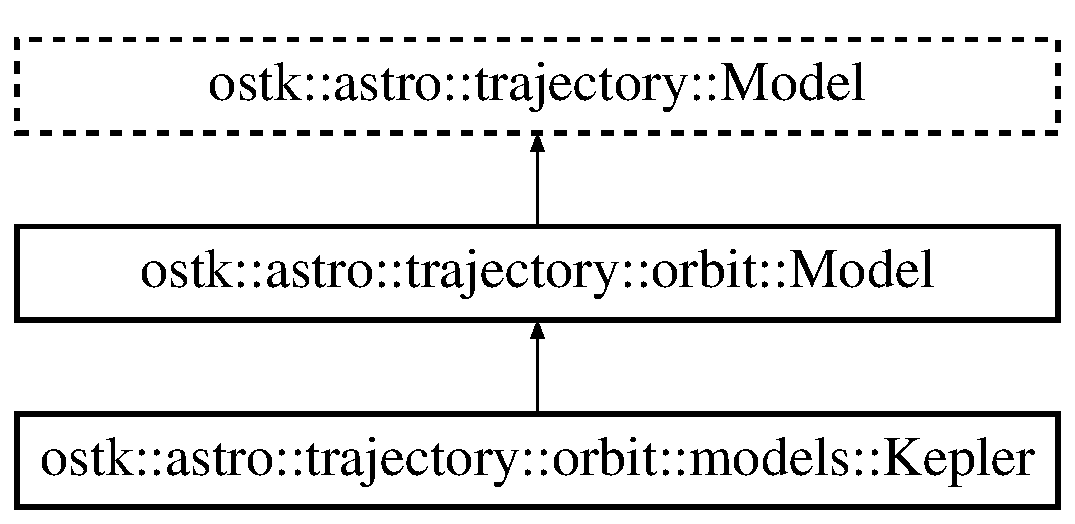
\includegraphics[height=3.000000cm]{classostk_1_1astro_1_1trajectory_1_1orbit_1_1models_1_1_kepler}
\end{center}
\end{figure}
\subsection*{Public Types}
\begin{DoxyCompactItemize}
\item 
enum \hyperlink{classostk_1_1astro_1_1trajectory_1_1orbit_1_1models_1_1_kepler_a3750f9177ff06a1938826e2c2881d5a9}{Perturbation\+Type} \{ \hyperlink{classostk_1_1astro_1_1trajectory_1_1orbit_1_1models_1_1_kepler_a3750f9177ff06a1938826e2c2881d5a9a6adf97f83acf6453d4a6a4b1070f3754}{Perturbation\+Type\+::\+None}, 
\hyperlink{classostk_1_1astro_1_1trajectory_1_1orbit_1_1models_1_1_kepler_a3750f9177ff06a1938826e2c2881d5a9a7f132d501fb9863844ab51697900d494}{Perturbation\+Type\+::\+J2}
 \}
\end{DoxyCompactItemize}
\subsection*{Public Member Functions}
\begin{DoxyCompactItemize}
\item 
\hyperlink{classostk_1_1astro_1_1trajectory_1_1orbit_1_1models_1_1_kepler_a9bf6dd4dbd63bb2551fa649b59ae297b}{Kepler} (const \hyperlink{classostk_1_1astro_1_1trajectory_1_1orbit_1_1models_1_1kepler_1_1_c_o_e}{C\+OE} \&a\+Classical\+Orbital\+Element\+Set, const Instant \&an\+Epoch, const Derived \&a\+Gravitational\+Parameter, const Length \&an\+Equatorial\+Radius, const Real \&a\+J2, const \hyperlink{classostk_1_1astro_1_1trajectory_1_1orbit_1_1models_1_1_kepler_a3750f9177ff06a1938826e2c2881d5a9}{Kepler\+::\+Perturbation\+Type} \&a\+Perturbation\+Type)
\item 
\hyperlink{classostk_1_1astro_1_1trajectory_1_1orbit_1_1models_1_1_kepler_afc95c7ec38bba8e24eba704c408523b6}{Kepler} (const \hyperlink{classostk_1_1astro_1_1trajectory_1_1orbit_1_1models_1_1kepler_1_1_c_o_e}{C\+OE} \&a\+Classical\+Orbital\+Element\+Set, const Instant \&an\+Epoch, const Celestial \&a\+Celestial\+Object, const \hyperlink{classostk_1_1astro_1_1trajectory_1_1orbit_1_1models_1_1_kepler_a3750f9177ff06a1938826e2c2881d5a9}{Kepler\+::\+Perturbation\+Type} \&a\+Perturbation\+Type, const bool in\+Fixed\+Frame=false)
\item 
virtual \hyperlink{classostk_1_1astro_1_1trajectory_1_1orbit_1_1models_1_1_kepler}{Kepler} $\ast$ \hyperlink{classostk_1_1astro_1_1trajectory_1_1orbit_1_1models_1_1_kepler_afb76b3571c73fb5c87129033f7d66520}{clone} () const override
\item 
bool \hyperlink{classostk_1_1astro_1_1trajectory_1_1orbit_1_1models_1_1_kepler_a0fa60d97287b75564e1e5a2390f137f4}{operator==} (const \hyperlink{classostk_1_1astro_1_1trajectory_1_1orbit_1_1models_1_1_kepler}{Kepler} \&a\+Keplerian\+Model) const
\item 
bool \hyperlink{classostk_1_1astro_1_1trajectory_1_1orbit_1_1models_1_1_kepler_aac43844f43000a181bf504529763bc82}{operator!=} (const \hyperlink{classostk_1_1astro_1_1trajectory_1_1orbit_1_1models_1_1_kepler}{Kepler} \&a\+Keplerian\+Model) const
\item 
virtual bool \hyperlink{classostk_1_1astro_1_1trajectory_1_1orbit_1_1models_1_1_kepler_a4c74402d5483a51e5e0fe1920cd52ec4}{is\+Defined} () const override
\item 
\hyperlink{classostk_1_1astro_1_1trajectory_1_1orbit_1_1models_1_1kepler_1_1_c_o_e}{C\+OE} \hyperlink{classostk_1_1astro_1_1trajectory_1_1orbit_1_1models_1_1_kepler_a1a5e2d4a27c4e20d91924a3a751cbba4}{get\+Classical\+Orbital\+Elements} () const
\item 
virtual Instant \hyperlink{classostk_1_1astro_1_1trajectory_1_1orbit_1_1models_1_1_kepler_a01551fd006896966d4d5e4442c182f92}{get\+Epoch} () const override
\item 
virtual Integer \hyperlink{classostk_1_1astro_1_1trajectory_1_1orbit_1_1models_1_1_kepler_a2aa5b94462f65ea7e703d319d3e028b3}{get\+Revolution\+Number\+At\+Epoch} () const override
\item 
Derived \hyperlink{classostk_1_1astro_1_1trajectory_1_1orbit_1_1models_1_1_kepler_af7e879bf88e9a388c86d836ac50d6a97}{get\+Gravitational\+Parameter} () const
\item 
Length \hyperlink{classostk_1_1astro_1_1trajectory_1_1orbit_1_1models_1_1_kepler_abd9cabfcb1a39b627d2809d3cb11dad8}{get\+Equatorial\+Radius} () const
\item 
Real \hyperlink{classostk_1_1astro_1_1trajectory_1_1orbit_1_1models_1_1_kepler_aeff5940802c7795d9d709a0fdf15fa64}{get\+J2} () const
\item 
\hyperlink{classostk_1_1astro_1_1trajectory_1_1orbit_1_1models_1_1_kepler_a3750f9177ff06a1938826e2c2881d5a9}{Kepler\+::\+Perturbation\+Type} \hyperlink{classostk_1_1astro_1_1trajectory_1_1orbit_1_1models_1_1_kepler_a8f6d00fe11481e9267aded6f9aeafb1a}{get\+Perturbation\+Type} () const
\item 
virtual \hyperlink{classostk_1_1astro_1_1trajectory_1_1_state}{State} \hyperlink{classostk_1_1astro_1_1trajectory_1_1orbit_1_1models_1_1_kepler_a4de0c3d7a2b37c1c2ab4d6e207339809}{calculate\+State\+At} (const Instant \&an\+Instant) const override
\item 
virtual Integer \hyperlink{classostk_1_1astro_1_1trajectory_1_1orbit_1_1models_1_1_kepler_a312fe4296eadcb00799ce9981b0c4f18}{calculate\+Revolution\+Number\+At} (const Instant \&an\+Instant) const override
\item 
virtual void \hyperlink{classostk_1_1astro_1_1trajectory_1_1orbit_1_1models_1_1_kepler_a9c71803234f356ade03453e3ae19ae94}{print} (std\+::ostream \&an\+Output\+Stream, bool display\+Decorator=true) const override
\end{DoxyCompactItemize}
\subsection*{Static Public Member Functions}
\begin{DoxyCompactItemize}
\item 
static String \hyperlink{classostk_1_1astro_1_1trajectory_1_1orbit_1_1models_1_1_kepler_ad780ed9b53e355ebef1597f86d30cf84}{String\+From\+Perturbation\+Type} (const \hyperlink{classostk_1_1astro_1_1trajectory_1_1orbit_1_1models_1_1_kepler_a3750f9177ff06a1938826e2c2881d5a9}{Kepler\+::\+Perturbation\+Type} \&a\+Perturbation\+Type)
\end{DoxyCompactItemize}
\subsection*{Protected Member Functions}
\begin{DoxyCompactItemize}
\item 
virtual bool \hyperlink{classostk_1_1astro_1_1trajectory_1_1orbit_1_1models_1_1_kepler_ad2a61eb0cbd9887fc2180dc0818c209e}{operator==} (const \hyperlink{classostk_1_1astro_1_1trajectory_1_1_model}{trajectory\+::\+Model} \&a\+Model) const override
\item 
virtual bool \hyperlink{classostk_1_1astro_1_1trajectory_1_1orbit_1_1models_1_1_kepler_ab343575a423c5cecea4b21fa79c80726}{operator!=} (const \hyperlink{classostk_1_1astro_1_1trajectory_1_1_model}{trajectory\+::\+Model} \&a\+Model) const override
\end{DoxyCompactItemize}
\subsection*{Friends}
\begin{DoxyCompactItemize}
\item 
std\+::ostream \& \hyperlink{classostk_1_1astro_1_1trajectory_1_1orbit_1_1models_1_1_kepler_aedb386ce32716dfb187f89b52b023f2b}{operator$<$$<$} (std\+::ostream \&an\+Output\+Stream, const \hyperlink{classostk_1_1astro_1_1trajectory_1_1orbit_1_1models_1_1_kepler}{Kepler} \&a\+Keplerian\+Model)
\end{DoxyCompactItemize}


\subsection{Member Enumeration Documentation}
\mbox{\Hypertarget{classostk_1_1astro_1_1trajectory_1_1orbit_1_1models_1_1_kepler_a3750f9177ff06a1938826e2c2881d5a9}\label{classostk_1_1astro_1_1trajectory_1_1orbit_1_1models_1_1_kepler_a3750f9177ff06a1938826e2c2881d5a9}} 
\index{ostk\+::astro\+::trajectory\+::orbit\+::models\+::\+Kepler@{ostk\+::astro\+::trajectory\+::orbit\+::models\+::\+Kepler}!Perturbation\+Type@{Perturbation\+Type}}
\index{Perturbation\+Type@{Perturbation\+Type}!ostk\+::astro\+::trajectory\+::orbit\+::models\+::\+Kepler@{ostk\+::astro\+::trajectory\+::orbit\+::models\+::\+Kepler}}
\subsubsection{\texorpdfstring{Perturbation\+Type}{PerturbationType}}
{\footnotesize\ttfamily enum \hyperlink{classostk_1_1astro_1_1trajectory_1_1orbit_1_1models_1_1_kepler_a3750f9177ff06a1938826e2c2881d5a9}{ostk\+::astro\+::trajectory\+::orbit\+::models\+::\+Kepler\+::\+Perturbation\+Type}\hspace{0.3cm}{\ttfamily [strong]}}

\begin{DoxyEnumFields}{Enumerator}
\raisebox{\heightof{T}}[0pt][0pt]{\index{None@{None}!ostk\+::astro\+::trajectory\+::orbit\+::models\+::\+Kepler@{ostk\+::astro\+::trajectory\+::orbit\+::models\+::\+Kepler}}\index{ostk\+::astro\+::trajectory\+::orbit\+::models\+::\+Kepler@{ostk\+::astro\+::trajectory\+::orbit\+::models\+::\+Kepler}!None@{None}}}\mbox{\Hypertarget{classostk_1_1astro_1_1trajectory_1_1orbit_1_1models_1_1_kepler_a3750f9177ff06a1938826e2c2881d5a9a6adf97f83acf6453d4a6a4b1070f3754}\label{classostk_1_1astro_1_1trajectory_1_1orbit_1_1models_1_1_kepler_a3750f9177ff06a1938826e2c2881d5a9a6adf97f83acf6453d4a6a4b1070f3754}} 
None&\\
\hline

\raisebox{\heightof{T}}[0pt][0pt]{\index{J2@{J2}!ostk\+::astro\+::trajectory\+::orbit\+::models\+::\+Kepler@{ostk\+::astro\+::trajectory\+::orbit\+::models\+::\+Kepler}}\index{ostk\+::astro\+::trajectory\+::orbit\+::models\+::\+Kepler@{ostk\+::astro\+::trajectory\+::orbit\+::models\+::\+Kepler}!J2@{J2}}}\mbox{\Hypertarget{classostk_1_1astro_1_1trajectory_1_1orbit_1_1models_1_1_kepler_a3750f9177ff06a1938826e2c2881d5a9a7f132d501fb9863844ab51697900d494}\label{classostk_1_1astro_1_1trajectory_1_1orbit_1_1models_1_1_kepler_a3750f9177ff06a1938826e2c2881d5a9a7f132d501fb9863844ab51697900d494}} 
J2&\\
\hline

\end{DoxyEnumFields}


\subsection{Constructor \& Destructor Documentation}
\mbox{\Hypertarget{classostk_1_1astro_1_1trajectory_1_1orbit_1_1models_1_1_kepler_a9bf6dd4dbd63bb2551fa649b59ae297b}\label{classostk_1_1astro_1_1trajectory_1_1orbit_1_1models_1_1_kepler_a9bf6dd4dbd63bb2551fa649b59ae297b}} 
\index{ostk\+::astro\+::trajectory\+::orbit\+::models\+::\+Kepler@{ostk\+::astro\+::trajectory\+::orbit\+::models\+::\+Kepler}!Kepler@{Kepler}}
\index{Kepler@{Kepler}!ostk\+::astro\+::trajectory\+::orbit\+::models\+::\+Kepler@{ostk\+::astro\+::trajectory\+::orbit\+::models\+::\+Kepler}}
\subsubsection{\texorpdfstring{Kepler()}{Kepler()}\hspace{0.1cm}{\footnotesize\ttfamily [1/2]}}
{\footnotesize\ttfamily ostk\+::astro\+::trajectory\+::orbit\+::models\+::\+Kepler\+::\+Kepler (\begin{DoxyParamCaption}\item[{const \hyperlink{classostk_1_1astro_1_1trajectory_1_1orbit_1_1models_1_1kepler_1_1_c_o_e}{C\+OE} \&}]{a\+Classical\+Orbital\+Element\+Set,  }\item[{const Instant \&}]{an\+Epoch,  }\item[{const Derived \&}]{a\+Gravitational\+Parameter,  }\item[{const Length \&}]{an\+Equatorial\+Radius,  }\item[{const Real \&}]{a\+J2,  }\item[{const \hyperlink{classostk_1_1astro_1_1trajectory_1_1orbit_1_1models_1_1_kepler_a3750f9177ff06a1938826e2c2881d5a9}{Kepler\+::\+Perturbation\+Type} \&}]{a\+Perturbation\+Type }\end{DoxyParamCaption})}

\mbox{\Hypertarget{classostk_1_1astro_1_1trajectory_1_1orbit_1_1models_1_1_kepler_afc95c7ec38bba8e24eba704c408523b6}\label{classostk_1_1astro_1_1trajectory_1_1orbit_1_1models_1_1_kepler_afc95c7ec38bba8e24eba704c408523b6}} 
\index{ostk\+::astro\+::trajectory\+::orbit\+::models\+::\+Kepler@{ostk\+::astro\+::trajectory\+::orbit\+::models\+::\+Kepler}!Kepler@{Kepler}}
\index{Kepler@{Kepler}!ostk\+::astro\+::trajectory\+::orbit\+::models\+::\+Kepler@{ostk\+::astro\+::trajectory\+::orbit\+::models\+::\+Kepler}}
\subsubsection{\texorpdfstring{Kepler()}{Kepler()}\hspace{0.1cm}{\footnotesize\ttfamily [2/2]}}
{\footnotesize\ttfamily ostk\+::astro\+::trajectory\+::orbit\+::models\+::\+Kepler\+::\+Kepler (\begin{DoxyParamCaption}\item[{const \hyperlink{classostk_1_1astro_1_1trajectory_1_1orbit_1_1models_1_1kepler_1_1_c_o_e}{C\+OE} \&}]{a\+Classical\+Orbital\+Element\+Set,  }\item[{const Instant \&}]{an\+Epoch,  }\item[{const Celestial \&}]{a\+Celestial\+Object,  }\item[{const \hyperlink{classostk_1_1astro_1_1trajectory_1_1orbit_1_1models_1_1_kepler_a3750f9177ff06a1938826e2c2881d5a9}{Kepler\+::\+Perturbation\+Type} \&}]{a\+Perturbation\+Type,  }\item[{const bool}]{in\+Fixed\+Frame = {\ttfamily false} }\end{DoxyParamCaption})}



\subsection{Member Function Documentation}
\mbox{\Hypertarget{classostk_1_1astro_1_1trajectory_1_1orbit_1_1models_1_1_kepler_a312fe4296eadcb00799ce9981b0c4f18}\label{classostk_1_1astro_1_1trajectory_1_1orbit_1_1models_1_1_kepler_a312fe4296eadcb00799ce9981b0c4f18}} 
\index{ostk\+::astro\+::trajectory\+::orbit\+::models\+::\+Kepler@{ostk\+::astro\+::trajectory\+::orbit\+::models\+::\+Kepler}!calculate\+Revolution\+Number\+At@{calculate\+Revolution\+Number\+At}}
\index{calculate\+Revolution\+Number\+At@{calculate\+Revolution\+Number\+At}!ostk\+::astro\+::trajectory\+::orbit\+::models\+::\+Kepler@{ostk\+::astro\+::trajectory\+::orbit\+::models\+::\+Kepler}}
\subsubsection{\texorpdfstring{calculate\+Revolution\+Number\+At()}{calculateRevolutionNumberAt()}}
{\footnotesize\ttfamily Integer ostk\+::astro\+::trajectory\+::orbit\+::models\+::\+Kepler\+::calculate\+Revolution\+Number\+At (\begin{DoxyParamCaption}\item[{const Instant \&}]{an\+Instant }\end{DoxyParamCaption}) const\hspace{0.3cm}{\ttfamily [override]}, {\ttfamily [virtual]}}



Implements \hyperlink{classostk_1_1astro_1_1trajectory_1_1orbit_1_1_model_aeecf4cc22fa9c766801936c468cc52ac}{ostk\+::astro\+::trajectory\+::orbit\+::\+Model}.

\mbox{\Hypertarget{classostk_1_1astro_1_1trajectory_1_1orbit_1_1models_1_1_kepler_a4de0c3d7a2b37c1c2ab4d6e207339809}\label{classostk_1_1astro_1_1trajectory_1_1orbit_1_1models_1_1_kepler_a4de0c3d7a2b37c1c2ab4d6e207339809}} 
\index{ostk\+::astro\+::trajectory\+::orbit\+::models\+::\+Kepler@{ostk\+::astro\+::trajectory\+::orbit\+::models\+::\+Kepler}!calculate\+State\+At@{calculate\+State\+At}}
\index{calculate\+State\+At@{calculate\+State\+At}!ostk\+::astro\+::trajectory\+::orbit\+::models\+::\+Kepler@{ostk\+::astro\+::trajectory\+::orbit\+::models\+::\+Kepler}}
\subsubsection{\texorpdfstring{calculate\+State\+At()}{calculateStateAt()}}
{\footnotesize\ttfamily \hyperlink{classostk_1_1astro_1_1trajectory_1_1_state}{State} ostk\+::astro\+::trajectory\+::orbit\+::models\+::\+Kepler\+::calculate\+State\+At (\begin{DoxyParamCaption}\item[{const Instant \&}]{an\+Instant }\end{DoxyParamCaption}) const\hspace{0.3cm}{\ttfamily [override]}, {\ttfamily [virtual]}}



Implements \hyperlink{classostk_1_1astro_1_1trajectory_1_1orbit_1_1_model_a34a0d8979ec1f7ade3e434fc0dad3711}{ostk\+::astro\+::trajectory\+::orbit\+::\+Model}.

\mbox{\Hypertarget{classostk_1_1astro_1_1trajectory_1_1orbit_1_1models_1_1_kepler_afb76b3571c73fb5c87129033f7d66520}\label{classostk_1_1astro_1_1trajectory_1_1orbit_1_1models_1_1_kepler_afb76b3571c73fb5c87129033f7d66520}} 
\index{ostk\+::astro\+::trajectory\+::orbit\+::models\+::\+Kepler@{ostk\+::astro\+::trajectory\+::orbit\+::models\+::\+Kepler}!clone@{clone}}
\index{clone@{clone}!ostk\+::astro\+::trajectory\+::orbit\+::models\+::\+Kepler@{ostk\+::astro\+::trajectory\+::orbit\+::models\+::\+Kepler}}
\subsubsection{\texorpdfstring{clone()}{clone()}}
{\footnotesize\ttfamily \hyperlink{classostk_1_1astro_1_1trajectory_1_1orbit_1_1models_1_1_kepler}{Kepler} $\ast$ ostk\+::astro\+::trajectory\+::orbit\+::models\+::\+Kepler\+::clone (\begin{DoxyParamCaption}{ }\end{DoxyParamCaption}) const\hspace{0.3cm}{\ttfamily [override]}, {\ttfamily [virtual]}}



Implements \hyperlink{classostk_1_1astro_1_1trajectory_1_1orbit_1_1_model_a53dc07564e4c7c444da46360aa8ada15}{ostk\+::astro\+::trajectory\+::orbit\+::\+Model}.

\mbox{\Hypertarget{classostk_1_1astro_1_1trajectory_1_1orbit_1_1models_1_1_kepler_a1a5e2d4a27c4e20d91924a3a751cbba4}\label{classostk_1_1astro_1_1trajectory_1_1orbit_1_1models_1_1_kepler_a1a5e2d4a27c4e20d91924a3a751cbba4}} 
\index{ostk\+::astro\+::trajectory\+::orbit\+::models\+::\+Kepler@{ostk\+::astro\+::trajectory\+::orbit\+::models\+::\+Kepler}!get\+Classical\+Orbital\+Elements@{get\+Classical\+Orbital\+Elements}}
\index{get\+Classical\+Orbital\+Elements@{get\+Classical\+Orbital\+Elements}!ostk\+::astro\+::trajectory\+::orbit\+::models\+::\+Kepler@{ostk\+::astro\+::trajectory\+::orbit\+::models\+::\+Kepler}}
\subsubsection{\texorpdfstring{get\+Classical\+Orbital\+Elements()}{getClassicalOrbitalElements()}}
{\footnotesize\ttfamily \hyperlink{classostk_1_1astro_1_1trajectory_1_1orbit_1_1models_1_1kepler_1_1_c_o_e}{C\+OE} ostk\+::astro\+::trajectory\+::orbit\+::models\+::\+Kepler\+::get\+Classical\+Orbital\+Elements (\begin{DoxyParamCaption}{ }\end{DoxyParamCaption}) const}

\mbox{\Hypertarget{classostk_1_1astro_1_1trajectory_1_1orbit_1_1models_1_1_kepler_a01551fd006896966d4d5e4442c182f92}\label{classostk_1_1astro_1_1trajectory_1_1orbit_1_1models_1_1_kepler_a01551fd006896966d4d5e4442c182f92}} 
\index{ostk\+::astro\+::trajectory\+::orbit\+::models\+::\+Kepler@{ostk\+::astro\+::trajectory\+::orbit\+::models\+::\+Kepler}!get\+Epoch@{get\+Epoch}}
\index{get\+Epoch@{get\+Epoch}!ostk\+::astro\+::trajectory\+::orbit\+::models\+::\+Kepler@{ostk\+::astro\+::trajectory\+::orbit\+::models\+::\+Kepler}}
\subsubsection{\texorpdfstring{get\+Epoch()}{getEpoch()}}
{\footnotesize\ttfamily Instant ostk\+::astro\+::trajectory\+::orbit\+::models\+::\+Kepler\+::get\+Epoch (\begin{DoxyParamCaption}{ }\end{DoxyParamCaption}) const\hspace{0.3cm}{\ttfamily [override]}, {\ttfamily [virtual]}}



Implements \hyperlink{classostk_1_1astro_1_1trajectory_1_1orbit_1_1_model_a22055d5ab4c22e6177a3ddb8f45f1f9b}{ostk\+::astro\+::trajectory\+::orbit\+::\+Model}.

\mbox{\Hypertarget{classostk_1_1astro_1_1trajectory_1_1orbit_1_1models_1_1_kepler_abd9cabfcb1a39b627d2809d3cb11dad8}\label{classostk_1_1astro_1_1trajectory_1_1orbit_1_1models_1_1_kepler_abd9cabfcb1a39b627d2809d3cb11dad8}} 
\index{ostk\+::astro\+::trajectory\+::orbit\+::models\+::\+Kepler@{ostk\+::astro\+::trajectory\+::orbit\+::models\+::\+Kepler}!get\+Equatorial\+Radius@{get\+Equatorial\+Radius}}
\index{get\+Equatorial\+Radius@{get\+Equatorial\+Radius}!ostk\+::astro\+::trajectory\+::orbit\+::models\+::\+Kepler@{ostk\+::astro\+::trajectory\+::orbit\+::models\+::\+Kepler}}
\subsubsection{\texorpdfstring{get\+Equatorial\+Radius()}{getEquatorialRadius()}}
{\footnotesize\ttfamily Length ostk\+::astro\+::trajectory\+::orbit\+::models\+::\+Kepler\+::get\+Equatorial\+Radius (\begin{DoxyParamCaption}{ }\end{DoxyParamCaption}) const}

\mbox{\Hypertarget{classostk_1_1astro_1_1trajectory_1_1orbit_1_1models_1_1_kepler_af7e879bf88e9a388c86d836ac50d6a97}\label{classostk_1_1astro_1_1trajectory_1_1orbit_1_1models_1_1_kepler_af7e879bf88e9a388c86d836ac50d6a97}} 
\index{ostk\+::astro\+::trajectory\+::orbit\+::models\+::\+Kepler@{ostk\+::astro\+::trajectory\+::orbit\+::models\+::\+Kepler}!get\+Gravitational\+Parameter@{get\+Gravitational\+Parameter}}
\index{get\+Gravitational\+Parameter@{get\+Gravitational\+Parameter}!ostk\+::astro\+::trajectory\+::orbit\+::models\+::\+Kepler@{ostk\+::astro\+::trajectory\+::orbit\+::models\+::\+Kepler}}
\subsubsection{\texorpdfstring{get\+Gravitational\+Parameter()}{getGravitationalParameter()}}
{\footnotesize\ttfamily Derived ostk\+::astro\+::trajectory\+::orbit\+::models\+::\+Kepler\+::get\+Gravitational\+Parameter (\begin{DoxyParamCaption}{ }\end{DoxyParamCaption}) const}

\mbox{\Hypertarget{classostk_1_1astro_1_1trajectory_1_1orbit_1_1models_1_1_kepler_aeff5940802c7795d9d709a0fdf15fa64}\label{classostk_1_1astro_1_1trajectory_1_1orbit_1_1models_1_1_kepler_aeff5940802c7795d9d709a0fdf15fa64}} 
\index{ostk\+::astro\+::trajectory\+::orbit\+::models\+::\+Kepler@{ostk\+::astro\+::trajectory\+::orbit\+::models\+::\+Kepler}!get\+J2@{get\+J2}}
\index{get\+J2@{get\+J2}!ostk\+::astro\+::trajectory\+::orbit\+::models\+::\+Kepler@{ostk\+::astro\+::trajectory\+::orbit\+::models\+::\+Kepler}}
\subsubsection{\texorpdfstring{get\+J2()}{getJ2()}}
{\footnotesize\ttfamily Real ostk\+::astro\+::trajectory\+::orbit\+::models\+::\+Kepler\+::get\+J2 (\begin{DoxyParamCaption}{ }\end{DoxyParamCaption}) const}

\mbox{\Hypertarget{classostk_1_1astro_1_1trajectory_1_1orbit_1_1models_1_1_kepler_a8f6d00fe11481e9267aded6f9aeafb1a}\label{classostk_1_1astro_1_1trajectory_1_1orbit_1_1models_1_1_kepler_a8f6d00fe11481e9267aded6f9aeafb1a}} 
\index{ostk\+::astro\+::trajectory\+::orbit\+::models\+::\+Kepler@{ostk\+::astro\+::trajectory\+::orbit\+::models\+::\+Kepler}!get\+Perturbation\+Type@{get\+Perturbation\+Type}}
\index{get\+Perturbation\+Type@{get\+Perturbation\+Type}!ostk\+::astro\+::trajectory\+::orbit\+::models\+::\+Kepler@{ostk\+::astro\+::trajectory\+::orbit\+::models\+::\+Kepler}}
\subsubsection{\texorpdfstring{get\+Perturbation\+Type()}{getPerturbationType()}}
{\footnotesize\ttfamily \hyperlink{classostk_1_1astro_1_1trajectory_1_1orbit_1_1models_1_1_kepler_a3750f9177ff06a1938826e2c2881d5a9}{Kepler\+::\+Perturbation\+Type} ostk\+::astro\+::trajectory\+::orbit\+::models\+::\+Kepler\+::get\+Perturbation\+Type (\begin{DoxyParamCaption}{ }\end{DoxyParamCaption}) const}

\mbox{\Hypertarget{classostk_1_1astro_1_1trajectory_1_1orbit_1_1models_1_1_kepler_a2aa5b94462f65ea7e703d319d3e028b3}\label{classostk_1_1astro_1_1trajectory_1_1orbit_1_1models_1_1_kepler_a2aa5b94462f65ea7e703d319d3e028b3}} 
\index{ostk\+::astro\+::trajectory\+::orbit\+::models\+::\+Kepler@{ostk\+::astro\+::trajectory\+::orbit\+::models\+::\+Kepler}!get\+Revolution\+Number\+At\+Epoch@{get\+Revolution\+Number\+At\+Epoch}}
\index{get\+Revolution\+Number\+At\+Epoch@{get\+Revolution\+Number\+At\+Epoch}!ostk\+::astro\+::trajectory\+::orbit\+::models\+::\+Kepler@{ostk\+::astro\+::trajectory\+::orbit\+::models\+::\+Kepler}}
\subsubsection{\texorpdfstring{get\+Revolution\+Number\+At\+Epoch()}{getRevolutionNumberAtEpoch()}}
{\footnotesize\ttfamily Integer ostk\+::astro\+::trajectory\+::orbit\+::models\+::\+Kepler\+::get\+Revolution\+Number\+At\+Epoch (\begin{DoxyParamCaption}{ }\end{DoxyParamCaption}) const\hspace{0.3cm}{\ttfamily [override]}, {\ttfamily [virtual]}}



Implements \hyperlink{classostk_1_1astro_1_1trajectory_1_1orbit_1_1_model_af3f1866f86045da2c05efe4165735cf4}{ostk\+::astro\+::trajectory\+::orbit\+::\+Model}.

\mbox{\Hypertarget{classostk_1_1astro_1_1trajectory_1_1orbit_1_1models_1_1_kepler_a4c74402d5483a51e5e0fe1920cd52ec4}\label{classostk_1_1astro_1_1trajectory_1_1orbit_1_1models_1_1_kepler_a4c74402d5483a51e5e0fe1920cd52ec4}} 
\index{ostk\+::astro\+::trajectory\+::orbit\+::models\+::\+Kepler@{ostk\+::astro\+::trajectory\+::orbit\+::models\+::\+Kepler}!is\+Defined@{is\+Defined}}
\index{is\+Defined@{is\+Defined}!ostk\+::astro\+::trajectory\+::orbit\+::models\+::\+Kepler@{ostk\+::astro\+::trajectory\+::orbit\+::models\+::\+Kepler}}
\subsubsection{\texorpdfstring{is\+Defined()}{isDefined()}}
{\footnotesize\ttfamily bool ostk\+::astro\+::trajectory\+::orbit\+::models\+::\+Kepler\+::is\+Defined (\begin{DoxyParamCaption}{ }\end{DoxyParamCaption}) const\hspace{0.3cm}{\ttfamily [override]}, {\ttfamily [virtual]}}



Implements \hyperlink{classostk_1_1astro_1_1trajectory_1_1orbit_1_1_model_a13c5b5693dd86a072da0bd0e319bacc2}{ostk\+::astro\+::trajectory\+::orbit\+::\+Model}.

\mbox{\Hypertarget{classostk_1_1astro_1_1trajectory_1_1orbit_1_1models_1_1_kepler_aac43844f43000a181bf504529763bc82}\label{classostk_1_1astro_1_1trajectory_1_1orbit_1_1models_1_1_kepler_aac43844f43000a181bf504529763bc82}} 
\index{ostk\+::astro\+::trajectory\+::orbit\+::models\+::\+Kepler@{ostk\+::astro\+::trajectory\+::orbit\+::models\+::\+Kepler}!operator"!=@{operator"!=}}
\index{operator"!=@{operator"!=}!ostk\+::astro\+::trajectory\+::orbit\+::models\+::\+Kepler@{ostk\+::astro\+::trajectory\+::orbit\+::models\+::\+Kepler}}
\subsubsection{\texorpdfstring{operator"!=()}{operator!=()}\hspace{0.1cm}{\footnotesize\ttfamily [1/2]}}
{\footnotesize\ttfamily bool ostk\+::astro\+::trajectory\+::orbit\+::models\+::\+Kepler\+::operator!= (\begin{DoxyParamCaption}\item[{const \hyperlink{classostk_1_1astro_1_1trajectory_1_1orbit_1_1models_1_1_kepler}{Kepler} \&}]{a\+Keplerian\+Model }\end{DoxyParamCaption}) const}

\mbox{\Hypertarget{classostk_1_1astro_1_1trajectory_1_1orbit_1_1models_1_1_kepler_ab343575a423c5cecea4b21fa79c80726}\label{classostk_1_1astro_1_1trajectory_1_1orbit_1_1models_1_1_kepler_ab343575a423c5cecea4b21fa79c80726}} 
\index{ostk\+::astro\+::trajectory\+::orbit\+::models\+::\+Kepler@{ostk\+::astro\+::trajectory\+::orbit\+::models\+::\+Kepler}!operator"!=@{operator"!=}}
\index{operator"!=@{operator"!=}!ostk\+::astro\+::trajectory\+::orbit\+::models\+::\+Kepler@{ostk\+::astro\+::trajectory\+::orbit\+::models\+::\+Kepler}}
\subsubsection{\texorpdfstring{operator"!=()}{operator!=()}\hspace{0.1cm}{\footnotesize\ttfamily [2/2]}}
{\footnotesize\ttfamily bool ostk\+::astro\+::trajectory\+::orbit\+::models\+::\+Kepler\+::operator!= (\begin{DoxyParamCaption}\item[{const \hyperlink{classostk_1_1astro_1_1trajectory_1_1_model}{trajectory\+::\+Model} \&}]{a\+Model }\end{DoxyParamCaption}) const\hspace{0.3cm}{\ttfamily [override]}, {\ttfamily [protected]}, {\ttfamily [virtual]}}



Implements \hyperlink{classostk_1_1astro_1_1trajectory_1_1_model_a2dd77b9f6939d738f3a489f26c955340}{ostk\+::astro\+::trajectory\+::\+Model}.

\mbox{\Hypertarget{classostk_1_1astro_1_1trajectory_1_1orbit_1_1models_1_1_kepler_a0fa60d97287b75564e1e5a2390f137f4}\label{classostk_1_1astro_1_1trajectory_1_1orbit_1_1models_1_1_kepler_a0fa60d97287b75564e1e5a2390f137f4}} 
\index{ostk\+::astro\+::trajectory\+::orbit\+::models\+::\+Kepler@{ostk\+::astro\+::trajectory\+::orbit\+::models\+::\+Kepler}!operator==@{operator==}}
\index{operator==@{operator==}!ostk\+::astro\+::trajectory\+::orbit\+::models\+::\+Kepler@{ostk\+::astro\+::trajectory\+::orbit\+::models\+::\+Kepler}}
\subsubsection{\texorpdfstring{operator==()}{operator==()}\hspace{0.1cm}{\footnotesize\ttfamily [1/2]}}
{\footnotesize\ttfamily bool ostk\+::astro\+::trajectory\+::orbit\+::models\+::\+Kepler\+::operator== (\begin{DoxyParamCaption}\item[{const \hyperlink{classostk_1_1astro_1_1trajectory_1_1orbit_1_1models_1_1_kepler}{Kepler} \&}]{a\+Keplerian\+Model }\end{DoxyParamCaption}) const}

\mbox{\Hypertarget{classostk_1_1astro_1_1trajectory_1_1orbit_1_1models_1_1_kepler_ad2a61eb0cbd9887fc2180dc0818c209e}\label{classostk_1_1astro_1_1trajectory_1_1orbit_1_1models_1_1_kepler_ad2a61eb0cbd9887fc2180dc0818c209e}} 
\index{ostk\+::astro\+::trajectory\+::orbit\+::models\+::\+Kepler@{ostk\+::astro\+::trajectory\+::orbit\+::models\+::\+Kepler}!operator==@{operator==}}
\index{operator==@{operator==}!ostk\+::astro\+::trajectory\+::orbit\+::models\+::\+Kepler@{ostk\+::astro\+::trajectory\+::orbit\+::models\+::\+Kepler}}
\subsubsection{\texorpdfstring{operator==()}{operator==()}\hspace{0.1cm}{\footnotesize\ttfamily [2/2]}}
{\footnotesize\ttfamily bool ostk\+::astro\+::trajectory\+::orbit\+::models\+::\+Kepler\+::operator== (\begin{DoxyParamCaption}\item[{const \hyperlink{classostk_1_1astro_1_1trajectory_1_1_model}{trajectory\+::\+Model} \&}]{a\+Model }\end{DoxyParamCaption}) const\hspace{0.3cm}{\ttfamily [override]}, {\ttfamily [protected]}, {\ttfamily [virtual]}}



Implements \hyperlink{classostk_1_1astro_1_1trajectory_1_1_model_a874f79846e845859c070ce1b9874fc9c}{ostk\+::astro\+::trajectory\+::\+Model}.

\mbox{\Hypertarget{classostk_1_1astro_1_1trajectory_1_1orbit_1_1models_1_1_kepler_a9c71803234f356ade03453e3ae19ae94}\label{classostk_1_1astro_1_1trajectory_1_1orbit_1_1models_1_1_kepler_a9c71803234f356ade03453e3ae19ae94}} 
\index{ostk\+::astro\+::trajectory\+::orbit\+::models\+::\+Kepler@{ostk\+::astro\+::trajectory\+::orbit\+::models\+::\+Kepler}!print@{print}}
\index{print@{print}!ostk\+::astro\+::trajectory\+::orbit\+::models\+::\+Kepler@{ostk\+::astro\+::trajectory\+::orbit\+::models\+::\+Kepler}}
\subsubsection{\texorpdfstring{print()}{print()}}
{\footnotesize\ttfamily void ostk\+::astro\+::trajectory\+::orbit\+::models\+::\+Kepler\+::print (\begin{DoxyParamCaption}\item[{std\+::ostream \&}]{an\+Output\+Stream,  }\item[{bool}]{display\+Decorator = {\ttfamily true} }\end{DoxyParamCaption}) const\hspace{0.3cm}{\ttfamily [override]}, {\ttfamily [virtual]}}



Implements \hyperlink{classostk_1_1astro_1_1trajectory_1_1orbit_1_1_model_a8ea45c1a6e51a6153ce3f72f5294f0c6}{ostk\+::astro\+::trajectory\+::orbit\+::\+Model}.

\mbox{\Hypertarget{classostk_1_1astro_1_1trajectory_1_1orbit_1_1models_1_1_kepler_ad780ed9b53e355ebef1597f86d30cf84}\label{classostk_1_1astro_1_1trajectory_1_1orbit_1_1models_1_1_kepler_ad780ed9b53e355ebef1597f86d30cf84}} 
\index{ostk\+::astro\+::trajectory\+::orbit\+::models\+::\+Kepler@{ostk\+::astro\+::trajectory\+::orbit\+::models\+::\+Kepler}!String\+From\+Perturbation\+Type@{String\+From\+Perturbation\+Type}}
\index{String\+From\+Perturbation\+Type@{String\+From\+Perturbation\+Type}!ostk\+::astro\+::trajectory\+::orbit\+::models\+::\+Kepler@{ostk\+::astro\+::trajectory\+::orbit\+::models\+::\+Kepler}}
\subsubsection{\texorpdfstring{String\+From\+Perturbation\+Type()}{StringFromPerturbationType()}}
{\footnotesize\ttfamily String ostk\+::astro\+::trajectory\+::orbit\+::models\+::\+Kepler\+::\+String\+From\+Perturbation\+Type (\begin{DoxyParamCaption}\item[{const \hyperlink{classostk_1_1astro_1_1trajectory_1_1orbit_1_1models_1_1_kepler_a3750f9177ff06a1938826e2c2881d5a9}{Kepler\+::\+Perturbation\+Type} \&}]{a\+Perturbation\+Type }\end{DoxyParamCaption})\hspace{0.3cm}{\ttfamily [static]}}



\subsection{Friends And Related Function Documentation}
\mbox{\Hypertarget{classostk_1_1astro_1_1trajectory_1_1orbit_1_1models_1_1_kepler_aedb386ce32716dfb187f89b52b023f2b}\label{classostk_1_1astro_1_1trajectory_1_1orbit_1_1models_1_1_kepler_aedb386ce32716dfb187f89b52b023f2b}} 
\index{ostk\+::astro\+::trajectory\+::orbit\+::models\+::\+Kepler@{ostk\+::astro\+::trajectory\+::orbit\+::models\+::\+Kepler}!operator$<$$<$@{operator$<$$<$}}
\index{operator$<$$<$@{operator$<$$<$}!ostk\+::astro\+::trajectory\+::orbit\+::models\+::\+Kepler@{ostk\+::astro\+::trajectory\+::orbit\+::models\+::\+Kepler}}
\subsubsection{\texorpdfstring{operator$<$$<$}{operator<<}}
{\footnotesize\ttfamily std\+::ostream\& operator$<$$<$ (\begin{DoxyParamCaption}\item[{std\+::ostream \&}]{an\+Output\+Stream,  }\item[{const \hyperlink{classostk_1_1astro_1_1trajectory_1_1orbit_1_1models_1_1_kepler}{Kepler} \&}]{a\+Keplerian\+Model }\end{DoxyParamCaption})\hspace{0.3cm}{\ttfamily [friend]}}



The documentation for this class was generated from the following files\+:\begin{DoxyCompactItemize}
\item 
include/\+Open\+Space\+Toolkit/\+Astrodynamics/\+Trajectory/\+Orbit/\+Models/\hyperlink{_kepler_8hpp}{Kepler.\+hpp}\item 
src/\+Open\+Space\+Toolkit/\+Astrodynamics/\+Trajectory/\+Orbit/\+Models/\hyperlink{_kepler_8cpp}{Kepler.\+cpp}\end{DoxyCompactItemize}

\hypertarget{classostk_1_1astro_1_1trajectory_1_1orbit_1_1_model}{}\section{ostk\+:\+:astro\+:\+:trajectory\+:\+:orbit\+:\+:Model Class Reference}
\label{classostk_1_1astro_1_1trajectory_1_1orbit_1_1_model}\index{ostk\+::astro\+::trajectory\+::orbit\+::\+Model@{ostk\+::astro\+::trajectory\+::orbit\+::\+Model}}


{\ttfamily \#include $<$Model.\+hpp$>$}

Inheritance diagram for ostk\+:\+:astro\+:\+:trajectory\+:\+:orbit\+:\+:Model\+:\begin{figure}[H]
\begin{center}
\leavevmode
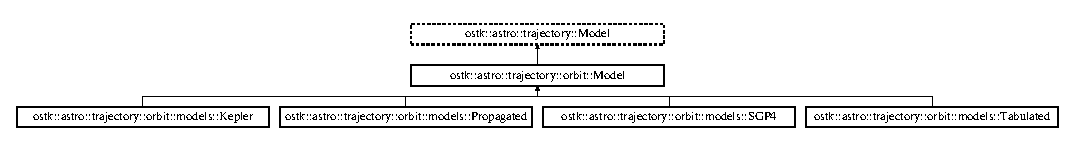
\includegraphics[height=1.484099cm]{classostk_1_1astro_1_1trajectory_1_1orbit_1_1_model}
\end{center}
\end{figure}
\subsection*{Public Member Functions}
\begin{DoxyCompactItemize}
\item 
\hyperlink{classostk_1_1astro_1_1trajectory_1_1orbit_1_1_model_a0604b5c1d0c0acb89cb42a10ea0fdb16}{Model} ()
\item 
virtual \hyperlink{classostk_1_1astro_1_1trajectory_1_1orbit_1_1_model_a7593c3eccd08104b00dd4d7c9c6a4d99}{$\sim$\+Model} ()=0
\item 
virtual \hyperlink{classostk_1_1astro_1_1trajectory_1_1orbit_1_1_model}{Model} $\ast$ \hyperlink{classostk_1_1astro_1_1trajectory_1_1orbit_1_1_model_a53dc07564e4c7c444da46360aa8ada15}{clone} () const =0
\item 
virtual bool \hyperlink{classostk_1_1astro_1_1trajectory_1_1orbit_1_1_model_a13c5b5693dd86a072da0bd0e319bacc2}{is\+Defined} () const =0
\item 
virtual Instant \hyperlink{classostk_1_1astro_1_1trajectory_1_1orbit_1_1_model_a22055d5ab4c22e6177a3ddb8f45f1f9b}{get\+Epoch} () const =0
\item 
virtual Integer \hyperlink{classostk_1_1astro_1_1trajectory_1_1orbit_1_1_model_af3f1866f86045da2c05efe4165735cf4}{get\+Revolution\+Number\+At\+Epoch} () const =0
\item 
virtual \hyperlink{classostk_1_1astro_1_1trajectory_1_1_state}{State} \hyperlink{classostk_1_1astro_1_1trajectory_1_1orbit_1_1_model_a34a0d8979ec1f7ade3e434fc0dad3711}{calculate\+State\+At} (const Instant \&an\+Instant) const =0
\item 
virtual Integer \hyperlink{classostk_1_1astro_1_1trajectory_1_1orbit_1_1_model_aeecf4cc22fa9c766801936c468cc52ac}{calculate\+Revolution\+Number\+At} (const Instant \&an\+Instant) const =0
\item 
virtual void \hyperlink{classostk_1_1astro_1_1trajectory_1_1orbit_1_1_model_a8ea45c1a6e51a6153ce3f72f5294f0c6}{print} (std\+::ostream \&an\+Output\+Stream, bool display\+Decorator=true) const =0
\end{DoxyCompactItemize}


\subsection{Constructor \& Destructor Documentation}
\mbox{\Hypertarget{classostk_1_1astro_1_1trajectory_1_1orbit_1_1_model_a0604b5c1d0c0acb89cb42a10ea0fdb16}\label{classostk_1_1astro_1_1trajectory_1_1orbit_1_1_model_a0604b5c1d0c0acb89cb42a10ea0fdb16}} 
\index{ostk\+::astro\+::trajectory\+::orbit\+::\+Model@{ostk\+::astro\+::trajectory\+::orbit\+::\+Model}!Model@{Model}}
\index{Model@{Model}!ostk\+::astro\+::trajectory\+::orbit\+::\+Model@{ostk\+::astro\+::trajectory\+::orbit\+::\+Model}}
\subsubsection{\texorpdfstring{Model()}{Model()}}
{\footnotesize\ttfamily ostk\+::astro\+::trajectory\+::orbit\+::\+Model\+::\+Model (\begin{DoxyParamCaption}{ }\end{DoxyParamCaption})}

\mbox{\Hypertarget{classostk_1_1astro_1_1trajectory_1_1orbit_1_1_model_a7593c3eccd08104b00dd4d7c9c6a4d99}\label{classostk_1_1astro_1_1trajectory_1_1orbit_1_1_model_a7593c3eccd08104b00dd4d7c9c6a4d99}} 
\index{ostk\+::astro\+::trajectory\+::orbit\+::\+Model@{ostk\+::astro\+::trajectory\+::orbit\+::\+Model}!````~Model@{$\sim$\+Model}}
\index{````~Model@{$\sim$\+Model}!ostk\+::astro\+::trajectory\+::orbit\+::\+Model@{ostk\+::astro\+::trajectory\+::orbit\+::\+Model}}
\subsubsection{\texorpdfstring{$\sim$\+Model()}{~Model()}}
{\footnotesize\ttfamily ostk\+::astro\+::trajectory\+::orbit\+::\+Model\+::$\sim$\+Model (\begin{DoxyParamCaption}{ }\end{DoxyParamCaption})\hspace{0.3cm}{\ttfamily [pure virtual]}}



Implements \hyperlink{classostk_1_1astro_1_1trajectory_1_1_model_a23acd7acccf729d8343180b83fe2f9f9}{ostk\+::astro\+::trajectory\+::\+Model}.



\subsection{Member Function Documentation}
\mbox{\Hypertarget{classostk_1_1astro_1_1trajectory_1_1orbit_1_1_model_aeecf4cc22fa9c766801936c468cc52ac}\label{classostk_1_1astro_1_1trajectory_1_1orbit_1_1_model_aeecf4cc22fa9c766801936c468cc52ac}} 
\index{ostk\+::astro\+::trajectory\+::orbit\+::\+Model@{ostk\+::astro\+::trajectory\+::orbit\+::\+Model}!calculate\+Revolution\+Number\+At@{calculate\+Revolution\+Number\+At}}
\index{calculate\+Revolution\+Number\+At@{calculate\+Revolution\+Number\+At}!ostk\+::astro\+::trajectory\+::orbit\+::\+Model@{ostk\+::astro\+::trajectory\+::orbit\+::\+Model}}
\subsubsection{\texorpdfstring{calculate\+Revolution\+Number\+At()}{calculateRevolutionNumberAt()}}
{\footnotesize\ttfamily virtual Integer ostk\+::astro\+::trajectory\+::orbit\+::\+Model\+::calculate\+Revolution\+Number\+At (\begin{DoxyParamCaption}\item[{const Instant \&}]{an\+Instant }\end{DoxyParamCaption}) const\hspace{0.3cm}{\ttfamily [pure virtual]}}



Implemented in \hyperlink{classostk_1_1astro_1_1trajectory_1_1orbit_1_1models_1_1_propagated_a6360392c65494aa42aadff58ec58e49c}{ostk\+::astro\+::trajectory\+::orbit\+::models\+::\+Propagated}, \hyperlink{classostk_1_1astro_1_1trajectory_1_1orbit_1_1models_1_1_kepler_a312fe4296eadcb00799ce9981b0c4f18}{ostk\+::astro\+::trajectory\+::orbit\+::models\+::\+Kepler}, \hyperlink{classostk_1_1astro_1_1trajectory_1_1orbit_1_1models_1_1_s_g_p4_af14e7851024d96eb20033ca9296dc003}{ostk\+::astro\+::trajectory\+::orbit\+::models\+::\+S\+G\+P4}, and \hyperlink{classostk_1_1astro_1_1trajectory_1_1orbit_1_1models_1_1_tabulated_ad7aabd8943ffaa16e569e331bdfa414e}{ostk\+::astro\+::trajectory\+::orbit\+::models\+::\+Tabulated}.

\mbox{\Hypertarget{classostk_1_1astro_1_1trajectory_1_1orbit_1_1_model_a34a0d8979ec1f7ade3e434fc0dad3711}\label{classostk_1_1astro_1_1trajectory_1_1orbit_1_1_model_a34a0d8979ec1f7ade3e434fc0dad3711}} 
\index{ostk\+::astro\+::trajectory\+::orbit\+::\+Model@{ostk\+::astro\+::trajectory\+::orbit\+::\+Model}!calculate\+State\+At@{calculate\+State\+At}}
\index{calculate\+State\+At@{calculate\+State\+At}!ostk\+::astro\+::trajectory\+::orbit\+::\+Model@{ostk\+::astro\+::trajectory\+::orbit\+::\+Model}}
\subsubsection{\texorpdfstring{calculate\+State\+At()}{calculateStateAt()}}
{\footnotesize\ttfamily virtual \hyperlink{classostk_1_1astro_1_1trajectory_1_1_state}{State} ostk\+::astro\+::trajectory\+::orbit\+::\+Model\+::calculate\+State\+At (\begin{DoxyParamCaption}\item[{const Instant \&}]{an\+Instant }\end{DoxyParamCaption}) const\hspace{0.3cm}{\ttfamily [pure virtual]}}



Implements \hyperlink{classostk_1_1astro_1_1trajectory_1_1_model_ad25eeaded2946bf73d44161b5f4e9a0e}{ostk\+::astro\+::trajectory\+::\+Model}.



Implemented in \hyperlink{classostk_1_1astro_1_1trajectory_1_1orbit_1_1models_1_1_propagated_a2efc3c1af735dcf2ec622d056fa0a13f}{ostk\+::astro\+::trajectory\+::orbit\+::models\+::\+Propagated}, \hyperlink{classostk_1_1astro_1_1trajectory_1_1orbit_1_1models_1_1_kepler_a4de0c3d7a2b37c1c2ab4d6e207339809}{ostk\+::astro\+::trajectory\+::orbit\+::models\+::\+Kepler}, \hyperlink{classostk_1_1astro_1_1trajectory_1_1orbit_1_1models_1_1_s_g_p4_ad88439d9c46a75d3da8c20d2872271e3}{ostk\+::astro\+::trajectory\+::orbit\+::models\+::\+S\+G\+P4}, and \hyperlink{classostk_1_1astro_1_1trajectory_1_1orbit_1_1models_1_1_tabulated_ad7935cafe71b572b97b9df93e469d2f8}{ostk\+::astro\+::trajectory\+::orbit\+::models\+::\+Tabulated}.

\mbox{\Hypertarget{classostk_1_1astro_1_1trajectory_1_1orbit_1_1_model_a53dc07564e4c7c444da46360aa8ada15}\label{classostk_1_1astro_1_1trajectory_1_1orbit_1_1_model_a53dc07564e4c7c444da46360aa8ada15}} 
\index{ostk\+::astro\+::trajectory\+::orbit\+::\+Model@{ostk\+::astro\+::trajectory\+::orbit\+::\+Model}!clone@{clone}}
\index{clone@{clone}!ostk\+::astro\+::trajectory\+::orbit\+::\+Model@{ostk\+::astro\+::trajectory\+::orbit\+::\+Model}}
\subsubsection{\texorpdfstring{clone()}{clone()}}
{\footnotesize\ttfamily virtual \hyperlink{classostk_1_1astro_1_1trajectory_1_1orbit_1_1_model}{Model}$\ast$ ostk\+::astro\+::trajectory\+::orbit\+::\+Model\+::clone (\begin{DoxyParamCaption}{ }\end{DoxyParamCaption}) const\hspace{0.3cm}{\ttfamily [pure virtual]}}



Implements \hyperlink{classostk_1_1astro_1_1trajectory_1_1_model_ad9f1467f711b07796ddc1437fb9ad9df}{ostk\+::astro\+::trajectory\+::\+Model}.



Implemented in \hyperlink{classostk_1_1astro_1_1trajectory_1_1orbit_1_1models_1_1_propagated_a283639d985495c05adb9e80edb91cd12}{ostk\+::astro\+::trajectory\+::orbit\+::models\+::\+Propagated}, \hyperlink{classostk_1_1astro_1_1trajectory_1_1orbit_1_1models_1_1_kepler_afb76b3571c73fb5c87129033f7d66520}{ostk\+::astro\+::trajectory\+::orbit\+::models\+::\+Kepler}, \hyperlink{classostk_1_1astro_1_1trajectory_1_1orbit_1_1models_1_1_s_g_p4_afb9928e09d66c13a77eb1126da6139eb}{ostk\+::astro\+::trajectory\+::orbit\+::models\+::\+S\+G\+P4}, and \hyperlink{classostk_1_1astro_1_1trajectory_1_1orbit_1_1models_1_1_tabulated_a53603727c33f9ff8db520831cf666142}{ostk\+::astro\+::trajectory\+::orbit\+::models\+::\+Tabulated}.

\mbox{\Hypertarget{classostk_1_1astro_1_1trajectory_1_1orbit_1_1_model_a22055d5ab4c22e6177a3ddb8f45f1f9b}\label{classostk_1_1astro_1_1trajectory_1_1orbit_1_1_model_a22055d5ab4c22e6177a3ddb8f45f1f9b}} 
\index{ostk\+::astro\+::trajectory\+::orbit\+::\+Model@{ostk\+::astro\+::trajectory\+::orbit\+::\+Model}!get\+Epoch@{get\+Epoch}}
\index{get\+Epoch@{get\+Epoch}!ostk\+::astro\+::trajectory\+::orbit\+::\+Model@{ostk\+::astro\+::trajectory\+::orbit\+::\+Model}}
\subsubsection{\texorpdfstring{get\+Epoch()}{getEpoch()}}
{\footnotesize\ttfamily virtual Instant ostk\+::astro\+::trajectory\+::orbit\+::\+Model\+::get\+Epoch (\begin{DoxyParamCaption}{ }\end{DoxyParamCaption}) const\hspace{0.3cm}{\ttfamily [pure virtual]}}



Implemented in \hyperlink{classostk_1_1astro_1_1trajectory_1_1orbit_1_1models_1_1_propagated_a3bf49ac0824e10057b6abca2cfcc692f}{ostk\+::astro\+::trajectory\+::orbit\+::models\+::\+Propagated}, \hyperlink{classostk_1_1astro_1_1trajectory_1_1orbit_1_1models_1_1_kepler_a01551fd006896966d4d5e4442c182f92}{ostk\+::astro\+::trajectory\+::orbit\+::models\+::\+Kepler}, \hyperlink{classostk_1_1astro_1_1trajectory_1_1orbit_1_1models_1_1_s_g_p4_af577ee4ad56452fe510d325a61a9792e}{ostk\+::astro\+::trajectory\+::orbit\+::models\+::\+S\+G\+P4}, and \hyperlink{classostk_1_1astro_1_1trajectory_1_1orbit_1_1models_1_1_tabulated_a0e92ebaac60e5113989eaadc66062b75}{ostk\+::astro\+::trajectory\+::orbit\+::models\+::\+Tabulated}.

\mbox{\Hypertarget{classostk_1_1astro_1_1trajectory_1_1orbit_1_1_model_af3f1866f86045da2c05efe4165735cf4}\label{classostk_1_1astro_1_1trajectory_1_1orbit_1_1_model_af3f1866f86045da2c05efe4165735cf4}} 
\index{ostk\+::astro\+::trajectory\+::orbit\+::\+Model@{ostk\+::astro\+::trajectory\+::orbit\+::\+Model}!get\+Revolution\+Number\+At\+Epoch@{get\+Revolution\+Number\+At\+Epoch}}
\index{get\+Revolution\+Number\+At\+Epoch@{get\+Revolution\+Number\+At\+Epoch}!ostk\+::astro\+::trajectory\+::orbit\+::\+Model@{ostk\+::astro\+::trajectory\+::orbit\+::\+Model}}
\subsubsection{\texorpdfstring{get\+Revolution\+Number\+At\+Epoch()}{getRevolutionNumberAtEpoch()}}
{\footnotesize\ttfamily virtual Integer ostk\+::astro\+::trajectory\+::orbit\+::\+Model\+::get\+Revolution\+Number\+At\+Epoch (\begin{DoxyParamCaption}{ }\end{DoxyParamCaption}) const\hspace{0.3cm}{\ttfamily [pure virtual]}}



Implemented in \hyperlink{classostk_1_1astro_1_1trajectory_1_1orbit_1_1models_1_1_propagated_a789e4236d2b8b212b1d978055b76abf1}{ostk\+::astro\+::trajectory\+::orbit\+::models\+::\+Propagated}, \hyperlink{classostk_1_1astro_1_1trajectory_1_1orbit_1_1models_1_1_kepler_a2aa5b94462f65ea7e703d319d3e028b3}{ostk\+::astro\+::trajectory\+::orbit\+::models\+::\+Kepler}, \hyperlink{classostk_1_1astro_1_1trajectory_1_1orbit_1_1models_1_1_s_g_p4_a6216f01c1ee37817ca1ae1c7036f942c}{ostk\+::astro\+::trajectory\+::orbit\+::models\+::\+S\+G\+P4}, and \hyperlink{classostk_1_1astro_1_1trajectory_1_1orbit_1_1models_1_1_tabulated_adbd37f167e43cedcb15358c16d62bae8}{ostk\+::astro\+::trajectory\+::orbit\+::models\+::\+Tabulated}.

\mbox{\Hypertarget{classostk_1_1astro_1_1trajectory_1_1orbit_1_1_model_a13c5b5693dd86a072da0bd0e319bacc2}\label{classostk_1_1astro_1_1trajectory_1_1orbit_1_1_model_a13c5b5693dd86a072da0bd0e319bacc2}} 
\index{ostk\+::astro\+::trajectory\+::orbit\+::\+Model@{ostk\+::astro\+::trajectory\+::orbit\+::\+Model}!is\+Defined@{is\+Defined}}
\index{is\+Defined@{is\+Defined}!ostk\+::astro\+::trajectory\+::orbit\+::\+Model@{ostk\+::astro\+::trajectory\+::orbit\+::\+Model}}
\subsubsection{\texorpdfstring{is\+Defined()}{isDefined()}}
{\footnotesize\ttfamily virtual bool ostk\+::astro\+::trajectory\+::orbit\+::\+Model\+::is\+Defined (\begin{DoxyParamCaption}{ }\end{DoxyParamCaption}) const\hspace{0.3cm}{\ttfamily [pure virtual]}}



Implements \hyperlink{classostk_1_1astro_1_1trajectory_1_1_model_a0d5cf6f754905f06c0ec1e39618c20a1}{ostk\+::astro\+::trajectory\+::\+Model}.



Implemented in \hyperlink{classostk_1_1astro_1_1trajectory_1_1orbit_1_1models_1_1_propagated_a530fd6bc017c74dedc43ced5fe843a03}{ostk\+::astro\+::trajectory\+::orbit\+::models\+::\+Propagated}, \hyperlink{classostk_1_1astro_1_1trajectory_1_1orbit_1_1models_1_1_kepler_a4c74402d5483a51e5e0fe1920cd52ec4}{ostk\+::astro\+::trajectory\+::orbit\+::models\+::\+Kepler}, \hyperlink{classostk_1_1astro_1_1trajectory_1_1orbit_1_1models_1_1_s_g_p4_ab18e0666588bd517c190942b1a54ed18}{ostk\+::astro\+::trajectory\+::orbit\+::models\+::\+S\+G\+P4}, and \hyperlink{classostk_1_1astro_1_1trajectory_1_1orbit_1_1models_1_1_tabulated_ad114ba4762b54211f74f0aa3ac5eedae}{ostk\+::astro\+::trajectory\+::orbit\+::models\+::\+Tabulated}.

\mbox{\Hypertarget{classostk_1_1astro_1_1trajectory_1_1orbit_1_1_model_a8ea45c1a6e51a6153ce3f72f5294f0c6}\label{classostk_1_1astro_1_1trajectory_1_1orbit_1_1_model_a8ea45c1a6e51a6153ce3f72f5294f0c6}} 
\index{ostk\+::astro\+::trajectory\+::orbit\+::\+Model@{ostk\+::astro\+::trajectory\+::orbit\+::\+Model}!print@{print}}
\index{print@{print}!ostk\+::astro\+::trajectory\+::orbit\+::\+Model@{ostk\+::astro\+::trajectory\+::orbit\+::\+Model}}
\subsubsection{\texorpdfstring{print()}{print()}}
{\footnotesize\ttfamily virtual void ostk\+::astro\+::trajectory\+::orbit\+::\+Model\+::print (\begin{DoxyParamCaption}\item[{std\+::ostream \&}]{an\+Output\+Stream,  }\item[{bool}]{display\+Decorator = {\ttfamily true} }\end{DoxyParamCaption}) const\hspace{0.3cm}{\ttfamily [pure virtual]}}



Implements \hyperlink{classostk_1_1astro_1_1trajectory_1_1_model_a4b2098483430a820481ed50b81656e31}{ostk\+::astro\+::trajectory\+::\+Model}.



Implemented in \hyperlink{classostk_1_1astro_1_1trajectory_1_1orbit_1_1models_1_1_propagated_a2b8aa6ff5511dbe92e6a3e7f4dd6880b}{ostk\+::astro\+::trajectory\+::orbit\+::models\+::\+Propagated}, \hyperlink{classostk_1_1astro_1_1trajectory_1_1orbit_1_1models_1_1_kepler_a9c71803234f356ade03453e3ae19ae94}{ostk\+::astro\+::trajectory\+::orbit\+::models\+::\+Kepler}, \hyperlink{classostk_1_1astro_1_1trajectory_1_1orbit_1_1models_1_1_s_g_p4_a12416476201382c3d1e3c620f7be106a}{ostk\+::astro\+::trajectory\+::orbit\+::models\+::\+S\+G\+P4}, and \hyperlink{classostk_1_1astro_1_1trajectory_1_1orbit_1_1models_1_1_tabulated_a66be3f1f23a464c666c38a3adcc3bab5}{ostk\+::astro\+::trajectory\+::orbit\+::models\+::\+Tabulated}.



The documentation for this class was generated from the following files\+:\begin{DoxyCompactItemize}
\item 
include/\+Open\+Space\+Toolkit/\+Astrodynamics/\+Trajectory/\+Orbit/\hyperlink{_orbit_2_model_8hpp}{Model.\+hpp}\item 
src/\+Open\+Space\+Toolkit/\+Astrodynamics/\+Trajectory/\+Orbit/\hyperlink{_orbit_2_model_8cpp}{Model.\+cpp}\end{DoxyCompactItemize}

\hypertarget{classostk_1_1astro_1_1trajectory_1_1_model}{}\section{ostk\+:\+:astro\+:\+:trajectory\+:\+:Model Class Reference}
\label{classostk_1_1astro_1_1trajectory_1_1_model}\index{ostk\+::astro\+::trajectory\+::\+Model@{ostk\+::astro\+::trajectory\+::\+Model}}


\hyperlink{classostk_1_1astro_1_1_trajectory}{Trajectory} model (abstract)  




{\ttfamily \#include $<$Model.\+hpp$>$}

Inheritance diagram for ostk\+:\+:astro\+:\+:trajectory\+:\+:Model\+:\begin{figure}[H]
\begin{center}
\leavevmode
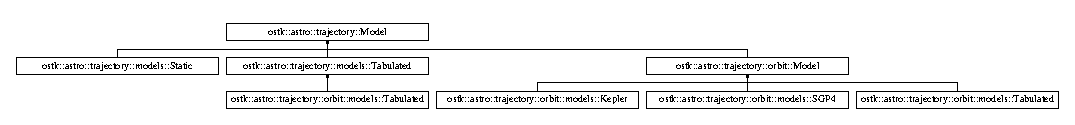
\includegraphics[height=0.989399cm]{classostk_1_1astro_1_1trajectory_1_1_model}
\end{center}
\end{figure}
\subsection*{Public Member Functions}
\begin{DoxyCompactItemize}
\item 
\hyperlink{classostk_1_1astro_1_1trajectory_1_1_model_aed4bcf4fbd44f69e97d8ff98112aa0f5}{Model} ()
\item 
virtual \hyperlink{classostk_1_1astro_1_1trajectory_1_1_model_a23acd7acccf729d8343180b83fe2f9f9}{$\sim$\+Model} ()=0
\item 
virtual \hyperlink{classostk_1_1astro_1_1trajectory_1_1_model}{Model} $\ast$ \hyperlink{classostk_1_1astro_1_1trajectory_1_1_model_ad9f1467f711b07796ddc1437fb9ad9df}{clone} () const =0
\item 
virtual bool \hyperlink{classostk_1_1astro_1_1trajectory_1_1_model_a874f79846e845859c070ce1b9874fc9c}{operator==} (const \hyperlink{classostk_1_1astro_1_1trajectory_1_1_model}{Model} \&a\+Model) const =0
\item 
virtual bool \hyperlink{classostk_1_1astro_1_1trajectory_1_1_model_a2dd77b9f6939d738f3a489f26c955340}{operator!=} (const \hyperlink{classostk_1_1astro_1_1trajectory_1_1_model}{Model} \&a\+Model) const =0
\item 
virtual bool \hyperlink{classostk_1_1astro_1_1trajectory_1_1_model_a0d5cf6f754905f06c0ec1e39618c20a1}{is\+Defined} () const =0
\item 
{\footnotesize template$<$class Type $>$ }\\bool \hyperlink{classostk_1_1astro_1_1trajectory_1_1_model_aedde1c01efbf407cca64b3f18b1a60f2}{is} () const
\begin{DoxyCompactList}\small\item\em Returns true if model can be converted to type. \end{DoxyCompactList}\item 
{\footnotesize template$<$class Type $>$ }\\const Type \& \hyperlink{classostk_1_1astro_1_1trajectory_1_1_model_a53365ee40062f5571b664998a56701e3}{as} () const
\begin{DoxyCompactList}\small\item\em \hyperlink{classostk_1_1astro_1_1_access}{Access} model as its underlying type. \end{DoxyCompactList}\item 
virtual \hyperlink{classostk_1_1astro_1_1trajectory_1_1_state}{State} \hyperlink{classostk_1_1astro_1_1trajectory_1_1_model_ad25eeaded2946bf73d44161b5f4e9a0e}{calculate\+State\+At} (const Instant \&an\+Instant) const =0
\item 
virtual Array$<$ \hyperlink{classostk_1_1astro_1_1trajectory_1_1_state}{State} $>$ \hyperlink{classostk_1_1astro_1_1trajectory_1_1_model_a3c3e4913aed2272174c0e6cd0d1a6415}{calculate\+States\+At} (const Array$<$ Instant $>$ \&an\+Instant\+Array) const
\item 
virtual void \hyperlink{classostk_1_1astro_1_1trajectory_1_1_model_a4b2098483430a820481ed50b81656e31}{print} (std\+::ostream \&an\+Output\+Stream, bool display\+Decorator=true) const =0
\end{DoxyCompactItemize}
\subsection*{Friends}
\begin{DoxyCompactItemize}
\item 
std\+::ostream \& \hyperlink{classostk_1_1astro_1_1trajectory_1_1_model_a68240493d08f91f6613186eb52823e85}{operator$<$$<$} (std\+::ostream \&an\+Output\+Stream, const \hyperlink{classostk_1_1astro_1_1trajectory_1_1_model}{Model} \&a\+Model)
\end{DoxyCompactItemize}


\subsection{Detailed Description}
\hyperlink{classostk_1_1astro_1_1_trajectory}{Trajectory} model (abstract) 

\subsection{Constructor \& Destructor Documentation}
\mbox{\Hypertarget{classostk_1_1astro_1_1trajectory_1_1_model_aed4bcf4fbd44f69e97d8ff98112aa0f5}\label{classostk_1_1astro_1_1trajectory_1_1_model_aed4bcf4fbd44f69e97d8ff98112aa0f5}} 
\index{ostk\+::astro\+::trajectory\+::\+Model@{ostk\+::astro\+::trajectory\+::\+Model}!Model@{Model}}
\index{Model@{Model}!ostk\+::astro\+::trajectory\+::\+Model@{ostk\+::astro\+::trajectory\+::\+Model}}
\subsubsection{\texorpdfstring{Model()}{Model()}}
{\footnotesize\ttfamily ostk\+::astro\+::trajectory\+::\+Model\+::\+Model (\begin{DoxyParamCaption}{ }\end{DoxyParamCaption})}

\mbox{\Hypertarget{classostk_1_1astro_1_1trajectory_1_1_model_a23acd7acccf729d8343180b83fe2f9f9}\label{classostk_1_1astro_1_1trajectory_1_1_model_a23acd7acccf729d8343180b83fe2f9f9}} 
\index{ostk\+::astro\+::trajectory\+::\+Model@{ostk\+::astro\+::trajectory\+::\+Model}!````~Model@{$\sim$\+Model}}
\index{````~Model@{$\sim$\+Model}!ostk\+::astro\+::trajectory\+::\+Model@{ostk\+::astro\+::trajectory\+::\+Model}}
\subsubsection{\texorpdfstring{$\sim$\+Model()}{~Model()}}
{\footnotesize\ttfamily ostk\+::astro\+::trajectory\+::\+Model\+::$\sim$\+Model (\begin{DoxyParamCaption}{ }\end{DoxyParamCaption})\hspace{0.3cm}{\ttfamily [pure virtual]}}



Implemented in \hyperlink{classostk_1_1astro_1_1trajectory_1_1orbit_1_1_model_a7593c3eccd08104b00dd4d7c9c6a4d99}{ostk\+::astro\+::trajectory\+::orbit\+::\+Model}.



\subsection{Member Function Documentation}
\mbox{\Hypertarget{classostk_1_1astro_1_1trajectory_1_1_model_a53365ee40062f5571b664998a56701e3}\label{classostk_1_1astro_1_1trajectory_1_1_model_a53365ee40062f5571b664998a56701e3}} 
\index{ostk\+::astro\+::trajectory\+::\+Model@{ostk\+::astro\+::trajectory\+::\+Model}!as@{as}}
\index{as@{as}!ostk\+::astro\+::trajectory\+::\+Model@{ostk\+::astro\+::trajectory\+::\+Model}}
\subsubsection{\texorpdfstring{as()}{as()}}
{\footnotesize\ttfamily template$<$class Type $>$ \\
const Type\& ostk\+::astro\+::trajectory\+::\+Model\+::as (\begin{DoxyParamCaption}{ }\end{DoxyParamCaption}) const\hspace{0.3cm}{\ttfamily [inline]}}



\hyperlink{classostk_1_1astro_1_1_access}{Access} model as its underlying type. 

\begin{DoxyReturn}{Returns}
Reference to underlying type 
\end{DoxyReturn}
\mbox{\Hypertarget{classostk_1_1astro_1_1trajectory_1_1_model_ad25eeaded2946bf73d44161b5f4e9a0e}\label{classostk_1_1astro_1_1trajectory_1_1_model_ad25eeaded2946bf73d44161b5f4e9a0e}} 
\index{ostk\+::astro\+::trajectory\+::\+Model@{ostk\+::astro\+::trajectory\+::\+Model}!calculate\+State\+At@{calculate\+State\+At}}
\index{calculate\+State\+At@{calculate\+State\+At}!ostk\+::astro\+::trajectory\+::\+Model@{ostk\+::astro\+::trajectory\+::\+Model}}
\subsubsection{\texorpdfstring{calculate\+State\+At()}{calculateStateAt()}}
{\footnotesize\ttfamily virtual \hyperlink{classostk_1_1astro_1_1trajectory_1_1_state}{State} ostk\+::astro\+::trajectory\+::\+Model\+::calculate\+State\+At (\begin{DoxyParamCaption}\item[{const Instant \&}]{an\+Instant }\end{DoxyParamCaption}) const\hspace{0.3cm}{\ttfamily [pure virtual]}}



Implemented in \hyperlink{classostk_1_1astro_1_1trajectory_1_1orbit_1_1models_1_1_propagated_a2efc3c1af735dcf2ec622d056fa0a13f}{ostk\+::astro\+::trajectory\+::orbit\+::models\+::\+Propagated}, \hyperlink{classostk_1_1astro_1_1trajectory_1_1orbit_1_1models_1_1_kepler_a4de0c3d7a2b37c1c2ab4d6e207339809}{ostk\+::astro\+::trajectory\+::orbit\+::models\+::\+Kepler}, \hyperlink{classostk_1_1astro_1_1trajectory_1_1orbit_1_1models_1_1_s_g_p4_ad88439d9c46a75d3da8c20d2872271e3}{ostk\+::astro\+::trajectory\+::orbit\+::models\+::\+S\+G\+P4}, \hyperlink{classostk_1_1astro_1_1trajectory_1_1models_1_1_tabulated_af2ebaa6456986636aa58c2f8666ed0b9}{ostk\+::astro\+::trajectory\+::models\+::\+Tabulated}, \hyperlink{classostk_1_1astro_1_1trajectory_1_1orbit_1_1models_1_1_tabulated_ad7935cafe71b572b97b9df93e469d2f8}{ostk\+::astro\+::trajectory\+::orbit\+::models\+::\+Tabulated}, \hyperlink{classostk_1_1astro_1_1trajectory_1_1models_1_1_static_a4297a74c953a105dc887a31227fbe1ff}{ostk\+::astro\+::trajectory\+::models\+::\+Static}, and \hyperlink{classostk_1_1astro_1_1trajectory_1_1orbit_1_1_model_a34a0d8979ec1f7ade3e434fc0dad3711}{ostk\+::astro\+::trajectory\+::orbit\+::\+Model}.

\mbox{\Hypertarget{classostk_1_1astro_1_1trajectory_1_1_model_a3c3e4913aed2272174c0e6cd0d1a6415}\label{classostk_1_1astro_1_1trajectory_1_1_model_a3c3e4913aed2272174c0e6cd0d1a6415}} 
\index{ostk\+::astro\+::trajectory\+::\+Model@{ostk\+::astro\+::trajectory\+::\+Model}!calculate\+States\+At@{calculate\+States\+At}}
\index{calculate\+States\+At@{calculate\+States\+At}!ostk\+::astro\+::trajectory\+::\+Model@{ostk\+::astro\+::trajectory\+::\+Model}}
\subsubsection{\texorpdfstring{calculate\+States\+At()}{calculateStatesAt()}}
{\footnotesize\ttfamily Array$<$ \hyperlink{classostk_1_1astro_1_1trajectory_1_1_state}{State} $>$ ostk\+::astro\+::trajectory\+::\+Model\+::calculate\+States\+At (\begin{DoxyParamCaption}\item[{const Array$<$ Instant $>$ \&}]{an\+Instant\+Array }\end{DoxyParamCaption}) const\hspace{0.3cm}{\ttfamily [virtual]}}



Reimplemented in \hyperlink{classostk_1_1astro_1_1trajectory_1_1orbit_1_1models_1_1_propagated_a9a4097432d2c863aedead23d2d67a7a7}{ostk\+::astro\+::trajectory\+::orbit\+::models\+::\+Propagated}.

\mbox{\Hypertarget{classostk_1_1astro_1_1trajectory_1_1_model_ad9f1467f711b07796ddc1437fb9ad9df}\label{classostk_1_1astro_1_1trajectory_1_1_model_ad9f1467f711b07796ddc1437fb9ad9df}} 
\index{ostk\+::astro\+::trajectory\+::\+Model@{ostk\+::astro\+::trajectory\+::\+Model}!clone@{clone}}
\index{clone@{clone}!ostk\+::astro\+::trajectory\+::\+Model@{ostk\+::astro\+::trajectory\+::\+Model}}
\subsubsection{\texorpdfstring{clone()}{clone()}}
{\footnotesize\ttfamily virtual \hyperlink{classostk_1_1astro_1_1trajectory_1_1_model}{Model}$\ast$ ostk\+::astro\+::trajectory\+::\+Model\+::clone (\begin{DoxyParamCaption}{ }\end{DoxyParamCaption}) const\hspace{0.3cm}{\ttfamily [pure virtual]}}



Implemented in \hyperlink{classostk_1_1astro_1_1trajectory_1_1orbit_1_1models_1_1_propagated_a283639d985495c05adb9e80edb91cd12}{ostk\+::astro\+::trajectory\+::orbit\+::models\+::\+Propagated}, \hyperlink{classostk_1_1astro_1_1trajectory_1_1orbit_1_1models_1_1_kepler_afb76b3571c73fb5c87129033f7d66520}{ostk\+::astro\+::trajectory\+::orbit\+::models\+::\+Kepler}, \hyperlink{classostk_1_1astro_1_1trajectory_1_1orbit_1_1models_1_1_s_g_p4_afb9928e09d66c13a77eb1126da6139eb}{ostk\+::astro\+::trajectory\+::orbit\+::models\+::\+S\+G\+P4}, \hyperlink{classostk_1_1astro_1_1trajectory_1_1models_1_1_tabulated_a553d2c4027ce269c1c2b3f4e9c65e14d}{ostk\+::astro\+::trajectory\+::models\+::\+Tabulated}, \hyperlink{classostk_1_1astro_1_1trajectory_1_1orbit_1_1models_1_1_tabulated_a53603727c33f9ff8db520831cf666142}{ostk\+::astro\+::trajectory\+::orbit\+::models\+::\+Tabulated}, \hyperlink{classostk_1_1astro_1_1trajectory_1_1models_1_1_static_abe3edbc72ae2f4fbd6c2593e2aa08755}{ostk\+::astro\+::trajectory\+::models\+::\+Static}, and \hyperlink{classostk_1_1astro_1_1trajectory_1_1orbit_1_1_model_a53dc07564e4c7c444da46360aa8ada15}{ostk\+::astro\+::trajectory\+::orbit\+::\+Model}.

\mbox{\Hypertarget{classostk_1_1astro_1_1trajectory_1_1_model_aedde1c01efbf407cca64b3f18b1a60f2}\label{classostk_1_1astro_1_1trajectory_1_1_model_aedde1c01efbf407cca64b3f18b1a60f2}} 
\index{ostk\+::astro\+::trajectory\+::\+Model@{ostk\+::astro\+::trajectory\+::\+Model}!is@{is}}
\index{is@{is}!ostk\+::astro\+::trajectory\+::\+Model@{ostk\+::astro\+::trajectory\+::\+Model}}
\subsubsection{\texorpdfstring{is()}{is()}}
{\footnotesize\ttfamily template$<$class Type $>$ \\
bool ostk\+::astro\+::trajectory\+::\+Model\+::is (\begin{DoxyParamCaption}{ }\end{DoxyParamCaption}) const\hspace{0.3cm}{\ttfamily [inline]}}



Returns true if model can be converted to type. 

\begin{DoxyReturn}{Returns}
True if model can be converted to type 
\end{DoxyReturn}
\mbox{\Hypertarget{classostk_1_1astro_1_1trajectory_1_1_model_a0d5cf6f754905f06c0ec1e39618c20a1}\label{classostk_1_1astro_1_1trajectory_1_1_model_a0d5cf6f754905f06c0ec1e39618c20a1}} 
\index{ostk\+::astro\+::trajectory\+::\+Model@{ostk\+::astro\+::trajectory\+::\+Model}!is\+Defined@{is\+Defined}}
\index{is\+Defined@{is\+Defined}!ostk\+::astro\+::trajectory\+::\+Model@{ostk\+::astro\+::trajectory\+::\+Model}}
\subsubsection{\texorpdfstring{is\+Defined()}{isDefined()}}
{\footnotesize\ttfamily virtual bool ostk\+::astro\+::trajectory\+::\+Model\+::is\+Defined (\begin{DoxyParamCaption}{ }\end{DoxyParamCaption}) const\hspace{0.3cm}{\ttfamily [pure virtual]}}



Implemented in \hyperlink{classostk_1_1astro_1_1trajectory_1_1orbit_1_1models_1_1_propagated_a530fd6bc017c74dedc43ced5fe843a03}{ostk\+::astro\+::trajectory\+::orbit\+::models\+::\+Propagated}, \hyperlink{classostk_1_1astro_1_1trajectory_1_1orbit_1_1models_1_1_kepler_a4c74402d5483a51e5e0fe1920cd52ec4}{ostk\+::astro\+::trajectory\+::orbit\+::models\+::\+Kepler}, \hyperlink{classostk_1_1astro_1_1trajectory_1_1orbit_1_1models_1_1_s_g_p4_ab18e0666588bd517c190942b1a54ed18}{ostk\+::astro\+::trajectory\+::orbit\+::models\+::\+S\+G\+P4}, \hyperlink{classostk_1_1astro_1_1trajectory_1_1models_1_1_tabulated_a379da4c10a738c3f4578042c9bae0c91}{ostk\+::astro\+::trajectory\+::models\+::\+Tabulated}, \hyperlink{classostk_1_1astro_1_1trajectory_1_1orbit_1_1models_1_1_tabulated_ad114ba4762b54211f74f0aa3ac5eedae}{ostk\+::astro\+::trajectory\+::orbit\+::models\+::\+Tabulated}, \hyperlink{classostk_1_1astro_1_1trajectory_1_1models_1_1_static_a5a80d75c9215af9b198c9f8653c5bc17}{ostk\+::astro\+::trajectory\+::models\+::\+Static}, and \hyperlink{classostk_1_1astro_1_1trajectory_1_1orbit_1_1_model_a13c5b5693dd86a072da0bd0e319bacc2}{ostk\+::astro\+::trajectory\+::orbit\+::\+Model}.

\mbox{\Hypertarget{classostk_1_1astro_1_1trajectory_1_1_model_a2dd77b9f6939d738f3a489f26c955340}\label{classostk_1_1astro_1_1trajectory_1_1_model_a2dd77b9f6939d738f3a489f26c955340}} 
\index{ostk\+::astro\+::trajectory\+::\+Model@{ostk\+::astro\+::trajectory\+::\+Model}!operator"!=@{operator"!=}}
\index{operator"!=@{operator"!=}!ostk\+::astro\+::trajectory\+::\+Model@{ostk\+::astro\+::trajectory\+::\+Model}}
\subsubsection{\texorpdfstring{operator"!=()}{operator!=()}}
{\footnotesize\ttfamily virtual bool ostk\+::astro\+::trajectory\+::\+Model\+::operator!= (\begin{DoxyParamCaption}\item[{const \hyperlink{classostk_1_1astro_1_1trajectory_1_1_model}{Model} \&}]{a\+Model }\end{DoxyParamCaption}) const\hspace{0.3cm}{\ttfamily [pure virtual]}}



Implemented in \hyperlink{classostk_1_1astro_1_1trajectory_1_1orbit_1_1models_1_1_propagated_aeffaddcde5540fd1226add8466415d08}{ostk\+::astro\+::trajectory\+::orbit\+::models\+::\+Propagated}, \hyperlink{classostk_1_1astro_1_1trajectory_1_1orbit_1_1models_1_1_kepler_ab343575a423c5cecea4b21fa79c80726}{ostk\+::astro\+::trajectory\+::orbit\+::models\+::\+Kepler}, \hyperlink{classostk_1_1astro_1_1trajectory_1_1orbit_1_1models_1_1_s_g_p4_a87441104e4e1c63356abe0632b56edb6}{ostk\+::astro\+::trajectory\+::orbit\+::models\+::\+S\+G\+P4}, \hyperlink{classostk_1_1astro_1_1trajectory_1_1models_1_1_tabulated_a5e047165eb79ea50d257c2cb1bafc30d}{ostk\+::astro\+::trajectory\+::models\+::\+Tabulated}, \hyperlink{classostk_1_1astro_1_1trajectory_1_1orbit_1_1models_1_1_tabulated_a17610dc24fefecd03ae595cc78ef3079}{ostk\+::astro\+::trajectory\+::orbit\+::models\+::\+Tabulated}, and \hyperlink{classostk_1_1astro_1_1trajectory_1_1models_1_1_static_af85efc113db69c75c1afc7db0e81297b}{ostk\+::astro\+::trajectory\+::models\+::\+Static}.

\mbox{\Hypertarget{classostk_1_1astro_1_1trajectory_1_1_model_a874f79846e845859c070ce1b9874fc9c}\label{classostk_1_1astro_1_1trajectory_1_1_model_a874f79846e845859c070ce1b9874fc9c}} 
\index{ostk\+::astro\+::trajectory\+::\+Model@{ostk\+::astro\+::trajectory\+::\+Model}!operator==@{operator==}}
\index{operator==@{operator==}!ostk\+::astro\+::trajectory\+::\+Model@{ostk\+::astro\+::trajectory\+::\+Model}}
\subsubsection{\texorpdfstring{operator==()}{operator==()}}
{\footnotesize\ttfamily virtual bool ostk\+::astro\+::trajectory\+::\+Model\+::operator== (\begin{DoxyParamCaption}\item[{const \hyperlink{classostk_1_1astro_1_1trajectory_1_1_model}{Model} \&}]{a\+Model }\end{DoxyParamCaption}) const\hspace{0.3cm}{\ttfamily [pure virtual]}}



Implemented in \hyperlink{classostk_1_1astro_1_1trajectory_1_1orbit_1_1models_1_1_propagated_a29b52ccf653fbd84699edab0f198f590}{ostk\+::astro\+::trajectory\+::orbit\+::models\+::\+Propagated}, \hyperlink{classostk_1_1astro_1_1trajectory_1_1orbit_1_1models_1_1_kepler_ad2a61eb0cbd9887fc2180dc0818c209e}{ostk\+::astro\+::trajectory\+::orbit\+::models\+::\+Kepler}, \hyperlink{classostk_1_1astro_1_1trajectory_1_1orbit_1_1models_1_1_s_g_p4_ad51d979b8b9b37251b6381cfe9df55ea}{ostk\+::astro\+::trajectory\+::orbit\+::models\+::\+S\+G\+P4}, \hyperlink{classostk_1_1astro_1_1trajectory_1_1models_1_1_tabulated_a9d206aee35ebabe4b36ddfc057142f16}{ostk\+::astro\+::trajectory\+::models\+::\+Tabulated}, \hyperlink{classostk_1_1astro_1_1trajectory_1_1orbit_1_1models_1_1_tabulated_abd72010cb413d8479c097376bfebaf56}{ostk\+::astro\+::trajectory\+::orbit\+::models\+::\+Tabulated}, and \hyperlink{classostk_1_1astro_1_1trajectory_1_1models_1_1_static_a0ef36b672baa80f522135d86f3b6bb9c}{ostk\+::astro\+::trajectory\+::models\+::\+Static}.

\mbox{\Hypertarget{classostk_1_1astro_1_1trajectory_1_1_model_a4b2098483430a820481ed50b81656e31}\label{classostk_1_1astro_1_1trajectory_1_1_model_a4b2098483430a820481ed50b81656e31}} 
\index{ostk\+::astro\+::trajectory\+::\+Model@{ostk\+::astro\+::trajectory\+::\+Model}!print@{print}}
\index{print@{print}!ostk\+::astro\+::trajectory\+::\+Model@{ostk\+::astro\+::trajectory\+::\+Model}}
\subsubsection{\texorpdfstring{print()}{print()}}
{\footnotesize\ttfamily virtual void ostk\+::astro\+::trajectory\+::\+Model\+::print (\begin{DoxyParamCaption}\item[{std\+::ostream \&}]{an\+Output\+Stream,  }\item[{bool}]{display\+Decorator = {\ttfamily true} }\end{DoxyParamCaption}) const\hspace{0.3cm}{\ttfamily [pure virtual]}}



Implemented in \hyperlink{classostk_1_1astro_1_1trajectory_1_1orbit_1_1models_1_1_propagated_a2b8aa6ff5511dbe92e6a3e7f4dd6880b}{ostk\+::astro\+::trajectory\+::orbit\+::models\+::\+Propagated}, \hyperlink{classostk_1_1astro_1_1trajectory_1_1orbit_1_1models_1_1_kepler_a9c71803234f356ade03453e3ae19ae94}{ostk\+::astro\+::trajectory\+::orbit\+::models\+::\+Kepler}, \hyperlink{classostk_1_1astro_1_1trajectory_1_1orbit_1_1models_1_1_s_g_p4_a12416476201382c3d1e3c620f7be106a}{ostk\+::astro\+::trajectory\+::orbit\+::models\+::\+S\+G\+P4}, \hyperlink{classostk_1_1astro_1_1trajectory_1_1models_1_1_tabulated_a330bfffa50eb77eb7f6d45cfec1e9e29}{ostk\+::astro\+::trajectory\+::models\+::\+Tabulated}, \hyperlink{classostk_1_1astro_1_1trajectory_1_1orbit_1_1models_1_1_tabulated_a66be3f1f23a464c666c38a3adcc3bab5}{ostk\+::astro\+::trajectory\+::orbit\+::models\+::\+Tabulated}, \hyperlink{classostk_1_1astro_1_1trajectory_1_1models_1_1_static_aae663f763324f081911ea47070c9f79f}{ostk\+::astro\+::trajectory\+::models\+::\+Static}, and \hyperlink{classostk_1_1astro_1_1trajectory_1_1orbit_1_1_model_a8ea45c1a6e51a6153ce3f72f5294f0c6}{ostk\+::astro\+::trajectory\+::orbit\+::\+Model}.



\subsection{Friends And Related Function Documentation}
\mbox{\Hypertarget{classostk_1_1astro_1_1trajectory_1_1_model_a68240493d08f91f6613186eb52823e85}\label{classostk_1_1astro_1_1trajectory_1_1_model_a68240493d08f91f6613186eb52823e85}} 
\index{ostk\+::astro\+::trajectory\+::\+Model@{ostk\+::astro\+::trajectory\+::\+Model}!operator$<$$<$@{operator$<$$<$}}
\index{operator$<$$<$@{operator$<$$<$}!ostk\+::astro\+::trajectory\+::\+Model@{ostk\+::astro\+::trajectory\+::\+Model}}
\subsubsection{\texorpdfstring{operator$<$$<$}{operator<<}}
{\footnotesize\ttfamily std\+::ostream\& operator$<$$<$ (\begin{DoxyParamCaption}\item[{std\+::ostream \&}]{an\+Output\+Stream,  }\item[{const \hyperlink{classostk_1_1astro_1_1trajectory_1_1_model}{Model} \&}]{a\+Model }\end{DoxyParamCaption})\hspace{0.3cm}{\ttfamily [friend]}}



The documentation for this class was generated from the following files\+:\begin{DoxyCompactItemize}
\item 
include/\+Open\+Space\+Toolkit/\+Astrodynamics/\+Trajectory/\hyperlink{_model_8hpp}{Model.\+hpp}\item 
src/\+Open\+Space\+Toolkit/\+Astrodynamics/\+Trajectory/\hyperlink{_model_8cpp}{Model.\+cpp}\end{DoxyCompactItemize}

\hypertarget{classostk_1_1astro_1_1trajectory_1_1_orbit}{}\section{ostk\+:\+:astro\+:\+:trajectory\+:\+:Orbit Class Reference}
\label{classostk_1_1astro_1_1trajectory_1_1_orbit}\index{ostk\+::astro\+::trajectory\+::\+Orbit@{ostk\+::astro\+::trajectory\+::\+Orbit}}


Gravitationally curved trajectory of an object.  




{\ttfamily \#include $<$Orbit.\+hpp$>$}

Inheritance diagram for ostk\+:\+:astro\+:\+:trajectory\+:\+:Orbit\+:\begin{figure}[H]
\begin{center}
\leavevmode
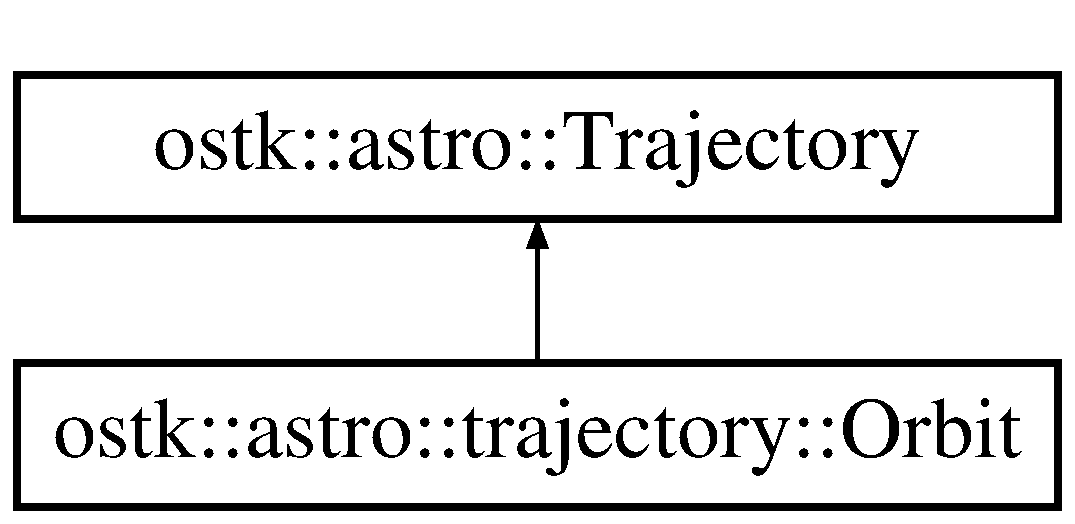
\includegraphics[height=2.000000cm]{classostk_1_1astro_1_1trajectory_1_1_orbit}
\end{center}
\end{figure}
\subsection*{Public Types}
\begin{DoxyCompactItemize}
\item 
enum \hyperlink{classostk_1_1astro_1_1trajectory_1_1_orbit_a1cc449ad56374471a8ab4300dde979e7}{Frame\+Type} \{ \newline
\hyperlink{classostk_1_1astro_1_1trajectory_1_1_orbit_a1cc449ad56374471a8ab4300dde979e7aec0fc0100c4fc1ce4eea230c3dc10360}{Frame\+Type\+::\+Undefined}, 
\hyperlink{classostk_1_1astro_1_1trajectory_1_1_orbit_a1cc449ad56374471a8ab4300dde979e7acd3459b28418fa8fa75ffaba4f3e7c74}{Frame\+Type\+::\+N\+ED}, 
\hyperlink{classostk_1_1astro_1_1trajectory_1_1_orbit_a1cc449ad56374471a8ab4300dde979e7acdfe4a5ed313c123b78c17d455cfa94f}{Frame\+Type\+::\+L\+V\+LH}, 
\hyperlink{classostk_1_1astro_1_1trajectory_1_1_orbit_a1cc449ad56374471a8ab4300dde979e7ae01a717c5a8a11cf57f7fdcb96aedc9c}{Frame\+Type\+::\+V\+V\+LH}, 
\newline
\hyperlink{classostk_1_1astro_1_1trajectory_1_1_orbit_a1cc449ad56374471a8ab4300dde979e7a9f24a174bf2de776f4f87caef847746f}{Frame\+Type\+::\+L\+V\+L\+H\+GD}, 
\hyperlink{classostk_1_1astro_1_1trajectory_1_1_orbit_a1cc449ad56374471a8ab4300dde979e7a4f190ed692b3a94eb49da59c497c7f55}{Frame\+Type\+::\+Q\+SW}, 
\hyperlink{classostk_1_1astro_1_1trajectory_1_1_orbit_a1cc449ad56374471a8ab4300dde979e7a6d951949ba8af28fa54a8629ec0f8f17}{Frame\+Type\+::\+T\+NW}, 
\hyperlink{classostk_1_1astro_1_1trajectory_1_1_orbit_a1cc449ad56374471a8ab4300dde979e7ac6a33911cc53df9bdb84aac8d86a0565}{Frame\+Type\+::\+V\+NC}
 \}
\item 
typedef Array$<$ \hyperlink{classostk_1_1astro_1_1trajectory_1_1orbit_1_1_pass}{Pass} $>$\+::Const\+Iterator \hyperlink{classostk_1_1astro_1_1trajectory_1_1_orbit_a0873dc63f4453eb2c07447e2774e944f}{Const\+Pass\+Iterator}
\end{DoxyCompactItemize}
\subsection*{Public Member Functions}
\begin{DoxyCompactItemize}
\item 
\hyperlink{classostk_1_1astro_1_1trajectory_1_1_orbit_aaccbf7c99f454ba6acd8aff68a2137bf}{Orbit} (const \hyperlink{classostk_1_1astro_1_1trajectory_1_1orbit_1_1_model}{orbit\+::\+Model} \&a\+Model, const Shared$<$ const Celestial $>$ \&a\+Celestial\+Object\+S\+Ptr)
\item 
\hyperlink{classostk_1_1astro_1_1trajectory_1_1_orbit_ac5396ec3866ad7afe7384bbfc4d41339}{Orbit} (const Array$<$ \hyperlink{classostk_1_1astro_1_1trajectory_1_1_state}{State} $>$ \&a\+State\+Array, const Integer \&an\+Initial\+Revolution\+Number, const Shared$<$ const Celestial $>$ \&a\+Celestial\+Object\+S\+Ptr)
\item 
\hyperlink{classostk_1_1astro_1_1trajectory_1_1_orbit_ac44603858b8379e0f2ded4236855c162}{Orbit} (const \hyperlink{classostk_1_1astro_1_1trajectory_1_1_orbit}{Orbit} \&an\+Orbit)
\item 
\hyperlink{classostk_1_1astro_1_1trajectory_1_1_orbit_aad56a0293156188474bcf1b78e55e249}{$\sim$\+Orbit} ()
\item 
\hyperlink{classostk_1_1astro_1_1trajectory_1_1_orbit}{Orbit} \& \hyperlink{classostk_1_1astro_1_1trajectory_1_1_orbit_a1a6ea873bd7728fcd1fdf028c5b2c026}{operator=} (const \hyperlink{classostk_1_1astro_1_1trajectory_1_1_orbit}{Orbit} \&an\+Orbit)=delete
\item 
bool \hyperlink{classostk_1_1astro_1_1trajectory_1_1_orbit_aa3fdab43c081059d268984dca953cb7d}{operator==} (const \hyperlink{classostk_1_1astro_1_1trajectory_1_1_orbit}{Orbit} \&an\+Orbit) const
\item 
bool \hyperlink{classostk_1_1astro_1_1trajectory_1_1_orbit_a9c376b2163bc4fcca62abccaf03014d2}{operator!=} (const \hyperlink{classostk_1_1astro_1_1trajectory_1_1_orbit}{Orbit} \&an\+Orbit) const
\item 
bool \hyperlink{classostk_1_1astro_1_1trajectory_1_1_orbit_abb1c3d611881104558aa93c9eb948455}{is\+Defined} () const
\item 
Integer \hyperlink{classostk_1_1astro_1_1trajectory_1_1_orbit_aa8ca190bd7b20f4654e0338660f57907}{get\+Revolution\+Number\+At} (const Instant \&an\+Instant) const
\item 
\hyperlink{classostk_1_1astro_1_1trajectory_1_1orbit_1_1_pass}{Pass} \hyperlink{classostk_1_1astro_1_1trajectory_1_1_orbit_a6cf47ea28cb2fb72a2659284a997b3b5}{get\+Pass\+At} (const Instant \&an\+Instant) const
\item 
\hyperlink{classostk_1_1astro_1_1trajectory_1_1orbit_1_1_pass}{Pass} \hyperlink{classostk_1_1astro_1_1trajectory_1_1_orbit_adee37553d5e3a67ab23f749c9147dd5c}{get\+Pass\+With\+Revolution\+Number} (const Integer \&a\+Revolution\+Number) const
\item 
Shared$<$ const Frame $>$ \hyperlink{classostk_1_1astro_1_1trajectory_1_1_orbit_a2549ae1a3ce8be76f441cfa85e9ab5ee}{get\+Orbital\+Frame} (const \hyperlink{classostk_1_1astro_1_1trajectory_1_1_orbit_a1cc449ad56374471a8ab4300dde979e7}{Orbit\+::\+Frame\+Type} \&a\+Frame\+Type) const
\item 
virtual void \hyperlink{classostk_1_1astro_1_1trajectory_1_1_orbit_ae890e832785f84c3f03c1e103f952826}{print} (std\+::ostream \&an\+Output\+Stream, bool display\+Decorator=true) const override
\begin{DoxyCompactList}\small\item\em Print trajectory to output stream. \end{DoxyCompactList}\end{DoxyCompactItemize}
\subsection*{Static Public Member Functions}
\begin{DoxyCompactItemize}
\item 
static \hyperlink{classostk_1_1astro_1_1trajectory_1_1_orbit}{Orbit} \hyperlink{classostk_1_1astro_1_1trajectory_1_1_orbit_a2b1bc936b69b8c70cd33a6b26c943f31}{Undefined} ()
\begin{DoxyCompactList}\small\item\em Constructs an undefined orbit. \end{DoxyCompactList}\item 
static \hyperlink{classostk_1_1astro_1_1trajectory_1_1_orbit}{Orbit} \hyperlink{classostk_1_1astro_1_1trajectory_1_1_orbit_aaf9d4274b72e4eb756212f7946edc237}{Circular} (const Instant \&an\+Epoch, const Length \&an\+Altitude, const Angle \&an\+Inclination, const Shared$<$ const Celestial $>$ \&a\+Celestial\+Object\+S\+Ptr)
\begin{DoxyCompactList}\small\item\em Constructs a circular orbit. \end{DoxyCompactList}\item 
static \hyperlink{classostk_1_1astro_1_1trajectory_1_1_orbit}{Orbit} \hyperlink{classostk_1_1astro_1_1trajectory_1_1_orbit_a88a5db265588461a9e756fd2aa4d3e4c}{Equatorial} (const Instant \&an\+Epoch, const Length \&an\+Apoapsis\+Altitude, const Length \&a\+Periapsis\+Altitude, const Shared$<$ const Celestial $>$ \&a\+Celestial\+Object\+S\+Ptr)
\begin{DoxyCompactList}\small\item\em Constructs an equatorial orbit. \end{DoxyCompactList}\item 
static \hyperlink{classostk_1_1astro_1_1trajectory_1_1_orbit}{Orbit} \hyperlink{classostk_1_1astro_1_1trajectory_1_1_orbit_a8070657a625af4dae7b79a23e5026dcd}{Circular\+Equatorial} (const Instant \&an\+Epoch, const Length \&an\+Altitude, const Shared$<$ const Celestial $>$ \&a\+Celestial\+Object\+S\+Ptr)
\begin{DoxyCompactList}\small\item\em Constructs a circular-\/equatorial orbit. \end{DoxyCompactList}\item 
static \hyperlink{classostk_1_1astro_1_1trajectory_1_1_orbit}{Orbit} \hyperlink{classostk_1_1astro_1_1trajectory_1_1_orbit_aaf0e7e3140ba78c06cc590f37ba680a5}{Sun\+Synchronous} (const Instant \&an\+Epoch, const Length \&an\+Altitude, const Time \&a\+Local\+Time\+At\+Descending\+Node, const Shared$<$ const Celestial $>$ \&a\+Celestial\+Object\+S\+Ptr)
\begin{DoxyCompactList}\small\item\em Constructs a Sun-\/synchronous orbit. \end{DoxyCompactList}\item 
static String \hyperlink{classostk_1_1astro_1_1trajectory_1_1_orbit_a329934037eb9eb4cacfcb2a5774753ed}{String\+From\+Frame\+Type} (const \hyperlink{classostk_1_1astro_1_1trajectory_1_1_orbit_a1cc449ad56374471a8ab4300dde979e7}{Orbit\+::\+Frame\+Type} \&a\+Frame\+Type)
\end{DoxyCompactItemize}


\subsection{Detailed Description}
Gravitationally curved trajectory of an object. 

https\+://en.wikipedia.\+org/wiki/\+Orbit 

\subsection{Member Typedef Documentation}
\mbox{\Hypertarget{classostk_1_1astro_1_1trajectory_1_1_orbit_a0873dc63f4453eb2c07447e2774e944f}\label{classostk_1_1astro_1_1trajectory_1_1_orbit_a0873dc63f4453eb2c07447e2774e944f}} 
\index{ostk\+::astro\+::trajectory\+::\+Orbit@{ostk\+::astro\+::trajectory\+::\+Orbit}!Const\+Pass\+Iterator@{Const\+Pass\+Iterator}}
\index{Const\+Pass\+Iterator@{Const\+Pass\+Iterator}!ostk\+::astro\+::trajectory\+::\+Orbit@{ostk\+::astro\+::trajectory\+::\+Orbit}}
\subsubsection{\texorpdfstring{Const\+Pass\+Iterator}{ConstPassIterator}}
{\footnotesize\ttfamily typedef Array$<$\hyperlink{classostk_1_1astro_1_1trajectory_1_1orbit_1_1_pass}{Pass}$>$\+::Const\+Iterator \hyperlink{classostk_1_1astro_1_1trajectory_1_1_orbit_a0873dc63f4453eb2c07447e2774e944f}{ostk\+::astro\+::trajectory\+::\+Orbit\+::\+Const\+Pass\+Iterator}}



\subsection{Member Enumeration Documentation}
\mbox{\Hypertarget{classostk_1_1astro_1_1trajectory_1_1_orbit_a1cc449ad56374471a8ab4300dde979e7}\label{classostk_1_1astro_1_1trajectory_1_1_orbit_a1cc449ad56374471a8ab4300dde979e7}} 
\index{ostk\+::astro\+::trajectory\+::\+Orbit@{ostk\+::astro\+::trajectory\+::\+Orbit}!Frame\+Type@{Frame\+Type}}
\index{Frame\+Type@{Frame\+Type}!ostk\+::astro\+::trajectory\+::\+Orbit@{ostk\+::astro\+::trajectory\+::\+Orbit}}
\subsubsection{\texorpdfstring{Frame\+Type}{FrameType}}
{\footnotesize\ttfamily enum \hyperlink{classostk_1_1astro_1_1trajectory_1_1_orbit_a1cc449ad56374471a8ab4300dde979e7}{ostk\+::astro\+::trajectory\+::\+Orbit\+::\+Frame\+Type}\hspace{0.3cm}{\ttfamily [strong]}}

\begin{DoxyEnumFields}{Enumerator}
\raisebox{\heightof{T}}[0pt][0pt]{\index{Undefined@{Undefined}!ostk\+::astro\+::trajectory\+::\+Orbit@{ostk\+::astro\+::trajectory\+::\+Orbit}}\index{ostk\+::astro\+::trajectory\+::\+Orbit@{ostk\+::astro\+::trajectory\+::\+Orbit}!Undefined@{Undefined}}}\mbox{\Hypertarget{classostk_1_1astro_1_1trajectory_1_1_orbit_a1cc449ad56374471a8ab4300dde979e7aec0fc0100c4fc1ce4eea230c3dc10360}\label{classostk_1_1astro_1_1trajectory_1_1_orbit_a1cc449ad56374471a8ab4300dde979e7aec0fc0100c4fc1ce4eea230c3dc10360}} 
Undefined&Undefined frame. \\
\hline

\raisebox{\heightof{T}}[0pt][0pt]{\index{N\+ED@{N\+ED}!ostk\+::astro\+::trajectory\+::\+Orbit@{ostk\+::astro\+::trajectory\+::\+Orbit}}\index{ostk\+::astro\+::trajectory\+::\+Orbit@{ostk\+::astro\+::trajectory\+::\+Orbit}!N\+ED@{N\+ED}}}\mbox{\Hypertarget{classostk_1_1astro_1_1trajectory_1_1_orbit_a1cc449ad56374471a8ab4300dde979e7acd3459b28418fa8fa75ffaba4f3e7c74}\label{classostk_1_1astro_1_1trajectory_1_1_orbit_a1cc449ad56374471a8ab4300dde979e7acd3459b28418fa8fa75ffaba4f3e7c74}} 
N\+ED&North-\/\+East-\/\+Down (N\+ED) frame. \\
\hline

\raisebox{\heightof{T}}[0pt][0pt]{\index{L\+V\+LH@{L\+V\+LH}!ostk\+::astro\+::trajectory\+::\+Orbit@{ostk\+::astro\+::trajectory\+::\+Orbit}}\index{ostk\+::astro\+::trajectory\+::\+Orbit@{ostk\+::astro\+::trajectory\+::\+Orbit}!L\+V\+LH@{L\+V\+LH}}}\mbox{\Hypertarget{classostk_1_1astro_1_1trajectory_1_1_orbit_a1cc449ad56374471a8ab4300dde979e7acdfe4a5ed313c123b78c17d455cfa94f}\label{classostk_1_1astro_1_1trajectory_1_1_orbit_a1cc449ad56374471a8ab4300dde979e7acdfe4a5ed313c123b78c17d455cfa94f}} 
L\+V\+LH&Local Vertical, Local Horizontal (L\+V\+LH) frame (X axis aligned with position, Z axis aligned with orbital momentum) \\
\hline

\raisebox{\heightof{T}}[0pt][0pt]{\index{V\+V\+LH@{V\+V\+LH}!ostk\+::astro\+::trajectory\+::\+Orbit@{ostk\+::astro\+::trajectory\+::\+Orbit}}\index{ostk\+::astro\+::trajectory\+::\+Orbit@{ostk\+::astro\+::trajectory\+::\+Orbit}!V\+V\+LH@{V\+V\+LH}}}\mbox{\Hypertarget{classostk_1_1astro_1_1trajectory_1_1_orbit_a1cc449ad56374471a8ab4300dde979e7ae01a717c5a8a11cf57f7fdcb96aedc9c}\label{classostk_1_1astro_1_1trajectory_1_1_orbit_a1cc449ad56374471a8ab4300dde979e7ae01a717c5a8a11cf57f7fdcb96aedc9c}} 
V\+V\+LH&Vehicle Velocity, Local Horizontal (V\+V\+LH) frame (Z axis aligned with opposite of position, Y axis aligned with opposite of orbital momentum) \\
\hline

\raisebox{\heightof{T}}[0pt][0pt]{\index{L\+V\+L\+H\+GD@{L\+V\+L\+H\+GD}!ostk\+::astro\+::trajectory\+::\+Orbit@{ostk\+::astro\+::trajectory\+::\+Orbit}}\index{ostk\+::astro\+::trajectory\+::\+Orbit@{ostk\+::astro\+::trajectory\+::\+Orbit}!L\+V\+L\+H\+GD@{L\+V\+L\+H\+GD}}}\mbox{\Hypertarget{classostk_1_1astro_1_1trajectory_1_1_orbit_a1cc449ad56374471a8ab4300dde979e7a9f24a174bf2de776f4f87caef847746f}\label{classostk_1_1astro_1_1trajectory_1_1_orbit_a1cc449ad56374471a8ab4300dde979e7a9f24a174bf2de776f4f87caef847746f}} 
L\+V\+L\+H\+GD&Local Vertical, Local Horizontal Geo\+Detic (L\+V\+L\+H\+GD) frame. \\
\hline

\raisebox{\heightof{T}}[0pt][0pt]{\index{Q\+SW@{Q\+SW}!ostk\+::astro\+::trajectory\+::\+Orbit@{ostk\+::astro\+::trajectory\+::\+Orbit}}\index{ostk\+::astro\+::trajectory\+::\+Orbit@{ostk\+::astro\+::trajectory\+::\+Orbit}!Q\+SW@{Q\+SW}}}\mbox{\Hypertarget{classostk_1_1astro_1_1trajectory_1_1_orbit_a1cc449ad56374471a8ab4300dde979e7a4f190ed692b3a94eb49da59c497c7f55}\label{classostk_1_1astro_1_1trajectory_1_1_orbit_a1cc449ad56374471a8ab4300dde979e7a4f190ed692b3a94eb49da59c497c7f55}} 
Q\+SW&Q\+SW frame (X axis aligned with position, Z axis aligned with orbital momentum) \\
\hline

\raisebox{\heightof{T}}[0pt][0pt]{\index{T\+NW@{T\+NW}!ostk\+::astro\+::trajectory\+::\+Orbit@{ostk\+::astro\+::trajectory\+::\+Orbit}}\index{ostk\+::astro\+::trajectory\+::\+Orbit@{ostk\+::astro\+::trajectory\+::\+Orbit}!T\+NW@{T\+NW}}}\mbox{\Hypertarget{classostk_1_1astro_1_1trajectory_1_1_orbit_a1cc449ad56374471a8ab4300dde979e7a6d951949ba8af28fa54a8629ec0f8f17}\label{classostk_1_1astro_1_1trajectory_1_1_orbit_a1cc449ad56374471a8ab4300dde979e7a6d951949ba8af28fa54a8629ec0f8f17}} 
T\+NW&T\+NW frame (X axis aligned with velocity, Z axis aligned with orbital momentum) \\
\hline

\raisebox{\heightof{T}}[0pt][0pt]{\index{V\+NC@{V\+NC}!ostk\+::astro\+::trajectory\+::\+Orbit@{ostk\+::astro\+::trajectory\+::\+Orbit}}\index{ostk\+::astro\+::trajectory\+::\+Orbit@{ostk\+::astro\+::trajectory\+::\+Orbit}!V\+NC@{V\+NC}}}\mbox{\Hypertarget{classostk_1_1astro_1_1trajectory_1_1_orbit_a1cc449ad56374471a8ab4300dde979e7ac6a33911cc53df9bdb84aac8d86a0565}\label{classostk_1_1astro_1_1trajectory_1_1_orbit_a1cc449ad56374471a8ab4300dde979e7ac6a33911cc53df9bdb84aac8d86a0565}} 
V\+NC&Velocity -\/ Normal -\/ Co-\/normal (V\+NC) frame (X axis aligned with velocity, Y axis aligned with orbital momentum) \\
\hline

\end{DoxyEnumFields}


\subsection{Constructor \& Destructor Documentation}
\mbox{\Hypertarget{classostk_1_1astro_1_1trajectory_1_1_orbit_aaccbf7c99f454ba6acd8aff68a2137bf}\label{classostk_1_1astro_1_1trajectory_1_1_orbit_aaccbf7c99f454ba6acd8aff68a2137bf}} 
\index{ostk\+::astro\+::trajectory\+::\+Orbit@{ostk\+::astro\+::trajectory\+::\+Orbit}!Orbit@{Orbit}}
\index{Orbit@{Orbit}!ostk\+::astro\+::trajectory\+::\+Orbit@{ostk\+::astro\+::trajectory\+::\+Orbit}}
\subsubsection{\texorpdfstring{Orbit()}{Orbit()}\hspace{0.1cm}{\footnotesize\ttfamily [1/3]}}
{\footnotesize\ttfamily ostk\+::astro\+::trajectory\+::\+Orbit\+::\+Orbit (\begin{DoxyParamCaption}\item[{const \hyperlink{classostk_1_1astro_1_1trajectory_1_1orbit_1_1_model}{orbit\+::\+Model} \&}]{a\+Model,  }\item[{const Shared$<$ const Celestial $>$ \&}]{a\+Celestial\+Object\+S\+Ptr }\end{DoxyParamCaption})}

\mbox{\Hypertarget{classostk_1_1astro_1_1trajectory_1_1_orbit_ac5396ec3866ad7afe7384bbfc4d41339}\label{classostk_1_1astro_1_1trajectory_1_1_orbit_ac5396ec3866ad7afe7384bbfc4d41339}} 
\index{ostk\+::astro\+::trajectory\+::\+Orbit@{ostk\+::astro\+::trajectory\+::\+Orbit}!Orbit@{Orbit}}
\index{Orbit@{Orbit}!ostk\+::astro\+::trajectory\+::\+Orbit@{ostk\+::astro\+::trajectory\+::\+Orbit}}
\subsubsection{\texorpdfstring{Orbit()}{Orbit()}\hspace{0.1cm}{\footnotesize\ttfamily [2/3]}}
{\footnotesize\ttfamily ostk\+::astro\+::trajectory\+::\+Orbit\+::\+Orbit (\begin{DoxyParamCaption}\item[{const Array$<$ \hyperlink{classostk_1_1astro_1_1trajectory_1_1_state}{State} $>$ \&}]{a\+State\+Array,  }\item[{const Integer \&}]{an\+Initial\+Revolution\+Number,  }\item[{const Shared$<$ const Celestial $>$ \&}]{a\+Celestial\+Object\+S\+Ptr }\end{DoxyParamCaption})}

\mbox{\Hypertarget{classostk_1_1astro_1_1trajectory_1_1_orbit_ac44603858b8379e0f2ded4236855c162}\label{classostk_1_1astro_1_1trajectory_1_1_orbit_ac44603858b8379e0f2ded4236855c162}} 
\index{ostk\+::astro\+::trajectory\+::\+Orbit@{ostk\+::astro\+::trajectory\+::\+Orbit}!Orbit@{Orbit}}
\index{Orbit@{Orbit}!ostk\+::astro\+::trajectory\+::\+Orbit@{ostk\+::astro\+::trajectory\+::\+Orbit}}
\subsubsection{\texorpdfstring{Orbit()}{Orbit()}\hspace{0.1cm}{\footnotesize\ttfamily [3/3]}}
{\footnotesize\ttfamily ostk\+::astro\+::trajectory\+::\+Orbit\+::\+Orbit (\begin{DoxyParamCaption}\item[{const \hyperlink{classostk_1_1astro_1_1trajectory_1_1_orbit}{Orbit} \&}]{an\+Orbit }\end{DoxyParamCaption})}

\mbox{\Hypertarget{classostk_1_1astro_1_1trajectory_1_1_orbit_aad56a0293156188474bcf1b78e55e249}\label{classostk_1_1astro_1_1trajectory_1_1_orbit_aad56a0293156188474bcf1b78e55e249}} 
\index{ostk\+::astro\+::trajectory\+::\+Orbit@{ostk\+::astro\+::trajectory\+::\+Orbit}!````~Orbit@{$\sim$\+Orbit}}
\index{````~Orbit@{$\sim$\+Orbit}!ostk\+::astro\+::trajectory\+::\+Orbit@{ostk\+::astro\+::trajectory\+::\+Orbit}}
\subsubsection{\texorpdfstring{$\sim$\+Orbit()}{~Orbit()}}
{\footnotesize\ttfamily ostk\+::astro\+::trajectory\+::\+Orbit\+::$\sim$\+Orbit (\begin{DoxyParamCaption}{ }\end{DoxyParamCaption})}



\subsection{Member Function Documentation}
\mbox{\Hypertarget{classostk_1_1astro_1_1trajectory_1_1_orbit_aaf9d4274b72e4eb756212f7946edc237}\label{classostk_1_1astro_1_1trajectory_1_1_orbit_aaf9d4274b72e4eb756212f7946edc237}} 
\index{ostk\+::astro\+::trajectory\+::\+Orbit@{ostk\+::astro\+::trajectory\+::\+Orbit}!Circular@{Circular}}
\index{Circular@{Circular}!ostk\+::astro\+::trajectory\+::\+Orbit@{ostk\+::astro\+::trajectory\+::\+Orbit}}
\subsubsection{\texorpdfstring{Circular()}{Circular()}}
{\footnotesize\ttfamily \hyperlink{classostk_1_1astro_1_1trajectory_1_1_orbit}{Orbit} ostk\+::astro\+::trajectory\+::\+Orbit\+::\+Circular (\begin{DoxyParamCaption}\item[{const Instant \&}]{an\+Epoch,  }\item[{const Length \&}]{an\+Altitude,  }\item[{const Angle \&}]{an\+Inclination,  }\item[{const Shared$<$ const Celestial $>$ \&}]{a\+Celestial\+Object\+S\+Ptr }\end{DoxyParamCaption})\hspace{0.3cm}{\ttfamily [static]}}



Constructs a circular orbit. 

\hyperlink{classostk_1_1astro_1_1trajectory_1_1_model}{Model}\+: Kepler (No Perturbation).


\begin{DoxyParams}[1]{Parameters}
\mbox{\tt in}  & {\em an\+Epoch} & An orbit epoch \\
\hline
\mbox{\tt in}  & {\em an\+Altitude} & An orbit altitude (wrt. equatorial radius) \\
\hline
\mbox{\tt in}  & {\em an\+Inclination} & An orbit inclination \\
\hline
\mbox{\tt in}  & {\em a\+Celestial\+Object\+S\+Ptr} & A shared pointer to a central celestial body \\
\hline
\end{DoxyParams}
\begin{DoxyReturn}{Returns}
Circular orbit 
\end{DoxyReturn}
\mbox{\Hypertarget{classostk_1_1astro_1_1trajectory_1_1_orbit_a8070657a625af4dae7b79a23e5026dcd}\label{classostk_1_1astro_1_1trajectory_1_1_orbit_a8070657a625af4dae7b79a23e5026dcd}} 
\index{ostk\+::astro\+::trajectory\+::\+Orbit@{ostk\+::astro\+::trajectory\+::\+Orbit}!Circular\+Equatorial@{Circular\+Equatorial}}
\index{Circular\+Equatorial@{Circular\+Equatorial}!ostk\+::astro\+::trajectory\+::\+Orbit@{ostk\+::astro\+::trajectory\+::\+Orbit}}
\subsubsection{\texorpdfstring{Circular\+Equatorial()}{CircularEquatorial()}}
{\footnotesize\ttfamily \hyperlink{classostk_1_1astro_1_1trajectory_1_1_orbit}{Orbit} ostk\+::astro\+::trajectory\+::\+Orbit\+::\+Circular\+Equatorial (\begin{DoxyParamCaption}\item[{const Instant \&}]{an\+Epoch,  }\item[{const Length \&}]{an\+Altitude,  }\item[{const Shared$<$ const Celestial $>$ \&}]{a\+Celestial\+Object\+S\+Ptr }\end{DoxyParamCaption})\hspace{0.3cm}{\ttfamily [static]}}



Constructs a circular-\/equatorial orbit. 

\hyperlink{classostk_1_1astro_1_1trajectory_1_1_model}{Model}\+: Kepler (No Perturbation).


\begin{DoxyParams}[1]{Parameters}
\mbox{\tt in}  & {\em an\+Epoch} & An orbit epoch \\
\hline
\mbox{\tt in}  & {\em an\+Altitude} & An orbit altitude (wrt. equatorial radius) \\
\hline
\mbox{\tt in}  & {\em a\+Celestial\+Object\+S\+Ptr} & A shared pointer to a central celestial body \\
\hline
\end{DoxyParams}
\begin{DoxyReturn}{Returns}
Circular-\/equatorial orbit 
\end{DoxyReturn}
\mbox{\Hypertarget{classostk_1_1astro_1_1trajectory_1_1_orbit_a88a5db265588461a9e756fd2aa4d3e4c}\label{classostk_1_1astro_1_1trajectory_1_1_orbit_a88a5db265588461a9e756fd2aa4d3e4c}} 
\index{ostk\+::astro\+::trajectory\+::\+Orbit@{ostk\+::astro\+::trajectory\+::\+Orbit}!Equatorial@{Equatorial}}
\index{Equatorial@{Equatorial}!ostk\+::astro\+::trajectory\+::\+Orbit@{ostk\+::astro\+::trajectory\+::\+Orbit}}
\subsubsection{\texorpdfstring{Equatorial()}{Equatorial()}}
{\footnotesize\ttfamily \hyperlink{classostk_1_1astro_1_1trajectory_1_1_orbit}{Orbit} ostk\+::astro\+::trajectory\+::\+Orbit\+::\+Equatorial (\begin{DoxyParamCaption}\item[{const Instant \&}]{an\+Epoch,  }\item[{const Length \&}]{an\+Apoapsis\+Altitude,  }\item[{const Length \&}]{a\+Periapsis\+Altitude,  }\item[{const Shared$<$ const Celestial $>$ \&}]{a\+Celestial\+Object\+S\+Ptr }\end{DoxyParamCaption})\hspace{0.3cm}{\ttfamily [static]}}



Constructs an equatorial orbit. 

\hyperlink{classostk_1_1astro_1_1trajectory_1_1_model}{Model}\+: Kepler (No Perturbation).


\begin{DoxyParams}[1]{Parameters}
\mbox{\tt in}  & {\em an\+Epoch} & An orbit epoch \\
\hline
\mbox{\tt in}  & {\em an\+Apoapsis\+Altitude} & An orbit apoapsis altitude (wrt. equatorial radius) \\
\hline
\mbox{\tt in}  & {\em a\+Periapsis\+Altitude} & An orbit periapsis altitude (wrt. equatorial radius) \\
\hline
\mbox{\tt in}  & {\em a\+Celestial\+Object\+S\+Ptr} & A shared pointer to a central celestial body \\
\hline
\end{DoxyParams}
\begin{DoxyReturn}{Returns}
Equatorial orbit 
\end{DoxyReturn}
\mbox{\Hypertarget{classostk_1_1astro_1_1trajectory_1_1_orbit_a2549ae1a3ce8be76f441cfa85e9ab5ee}\label{classostk_1_1astro_1_1trajectory_1_1_orbit_a2549ae1a3ce8be76f441cfa85e9ab5ee}} 
\index{ostk\+::astro\+::trajectory\+::\+Orbit@{ostk\+::astro\+::trajectory\+::\+Orbit}!get\+Orbital\+Frame@{get\+Orbital\+Frame}}
\index{get\+Orbital\+Frame@{get\+Orbital\+Frame}!ostk\+::astro\+::trajectory\+::\+Orbit@{ostk\+::astro\+::trajectory\+::\+Orbit}}
\subsubsection{\texorpdfstring{get\+Orbital\+Frame()}{getOrbitalFrame()}}
{\footnotesize\ttfamily Shared$<$ const Frame $>$ ostk\+::astro\+::trajectory\+::\+Orbit\+::get\+Orbital\+Frame (\begin{DoxyParamCaption}\item[{const \hyperlink{classostk_1_1astro_1_1trajectory_1_1_orbit_a1cc449ad56374471a8ab4300dde979e7}{Orbit\+::\+Frame\+Type} \&}]{a\+Frame\+Type }\end{DoxyParamCaption}) const}

\mbox{\Hypertarget{classostk_1_1astro_1_1trajectory_1_1_orbit_a6cf47ea28cb2fb72a2659284a997b3b5}\label{classostk_1_1astro_1_1trajectory_1_1_orbit_a6cf47ea28cb2fb72a2659284a997b3b5}} 
\index{ostk\+::astro\+::trajectory\+::\+Orbit@{ostk\+::astro\+::trajectory\+::\+Orbit}!get\+Pass\+At@{get\+Pass\+At}}
\index{get\+Pass\+At@{get\+Pass\+At}!ostk\+::astro\+::trajectory\+::\+Orbit@{ostk\+::astro\+::trajectory\+::\+Orbit}}
\subsubsection{\texorpdfstring{get\+Pass\+At()}{getPassAt()}}
{\footnotesize\ttfamily \hyperlink{classostk_1_1astro_1_1trajectory_1_1orbit_1_1_pass}{Pass} ostk\+::astro\+::trajectory\+::\+Orbit\+::get\+Pass\+At (\begin{DoxyParamCaption}\item[{const Instant \&}]{an\+Instant }\end{DoxyParamCaption}) const}

\mbox{\Hypertarget{classostk_1_1astro_1_1trajectory_1_1_orbit_adee37553d5e3a67ab23f749c9147dd5c}\label{classostk_1_1astro_1_1trajectory_1_1_orbit_adee37553d5e3a67ab23f749c9147dd5c}} 
\index{ostk\+::astro\+::trajectory\+::\+Orbit@{ostk\+::astro\+::trajectory\+::\+Orbit}!get\+Pass\+With\+Revolution\+Number@{get\+Pass\+With\+Revolution\+Number}}
\index{get\+Pass\+With\+Revolution\+Number@{get\+Pass\+With\+Revolution\+Number}!ostk\+::astro\+::trajectory\+::\+Orbit@{ostk\+::astro\+::trajectory\+::\+Orbit}}
\subsubsection{\texorpdfstring{get\+Pass\+With\+Revolution\+Number()}{getPassWithRevolutionNumber()}}
{\footnotesize\ttfamily \hyperlink{classostk_1_1astro_1_1trajectory_1_1orbit_1_1_pass}{Pass} ostk\+::astro\+::trajectory\+::\+Orbit\+::get\+Pass\+With\+Revolution\+Number (\begin{DoxyParamCaption}\item[{const Integer \&}]{a\+Revolution\+Number }\end{DoxyParamCaption}) const}

\mbox{\Hypertarget{classostk_1_1astro_1_1trajectory_1_1_orbit_aa8ca190bd7b20f4654e0338660f57907}\label{classostk_1_1astro_1_1trajectory_1_1_orbit_aa8ca190bd7b20f4654e0338660f57907}} 
\index{ostk\+::astro\+::trajectory\+::\+Orbit@{ostk\+::astro\+::trajectory\+::\+Orbit}!get\+Revolution\+Number\+At@{get\+Revolution\+Number\+At}}
\index{get\+Revolution\+Number\+At@{get\+Revolution\+Number\+At}!ostk\+::astro\+::trajectory\+::\+Orbit@{ostk\+::astro\+::trajectory\+::\+Orbit}}
\subsubsection{\texorpdfstring{get\+Revolution\+Number\+At()}{getRevolutionNumberAt()}}
{\footnotesize\ttfamily Integer ostk\+::astro\+::trajectory\+::\+Orbit\+::get\+Revolution\+Number\+At (\begin{DoxyParamCaption}\item[{const Instant \&}]{an\+Instant }\end{DoxyParamCaption}) const}

\mbox{\Hypertarget{classostk_1_1astro_1_1trajectory_1_1_orbit_abb1c3d611881104558aa93c9eb948455}\label{classostk_1_1astro_1_1trajectory_1_1_orbit_abb1c3d611881104558aa93c9eb948455}} 
\index{ostk\+::astro\+::trajectory\+::\+Orbit@{ostk\+::astro\+::trajectory\+::\+Orbit}!is\+Defined@{is\+Defined}}
\index{is\+Defined@{is\+Defined}!ostk\+::astro\+::trajectory\+::\+Orbit@{ostk\+::astro\+::trajectory\+::\+Orbit}}
\subsubsection{\texorpdfstring{is\+Defined()}{isDefined()}}
{\footnotesize\ttfamily bool ostk\+::astro\+::trajectory\+::\+Orbit\+::is\+Defined (\begin{DoxyParamCaption}{ }\end{DoxyParamCaption}) const}

\mbox{\Hypertarget{classostk_1_1astro_1_1trajectory_1_1_orbit_a9c376b2163bc4fcca62abccaf03014d2}\label{classostk_1_1astro_1_1trajectory_1_1_orbit_a9c376b2163bc4fcca62abccaf03014d2}} 
\index{ostk\+::astro\+::trajectory\+::\+Orbit@{ostk\+::astro\+::trajectory\+::\+Orbit}!operator"!=@{operator"!=}}
\index{operator"!=@{operator"!=}!ostk\+::astro\+::trajectory\+::\+Orbit@{ostk\+::astro\+::trajectory\+::\+Orbit}}
\subsubsection{\texorpdfstring{operator"!=()}{operator!=()}}
{\footnotesize\ttfamily bool ostk\+::astro\+::trajectory\+::\+Orbit\+::operator!= (\begin{DoxyParamCaption}\item[{const \hyperlink{classostk_1_1astro_1_1trajectory_1_1_orbit}{Orbit} \&}]{an\+Orbit }\end{DoxyParamCaption}) const}

\mbox{\Hypertarget{classostk_1_1astro_1_1trajectory_1_1_orbit_a1a6ea873bd7728fcd1fdf028c5b2c026}\label{classostk_1_1astro_1_1trajectory_1_1_orbit_a1a6ea873bd7728fcd1fdf028c5b2c026}} 
\index{ostk\+::astro\+::trajectory\+::\+Orbit@{ostk\+::astro\+::trajectory\+::\+Orbit}!operator=@{operator=}}
\index{operator=@{operator=}!ostk\+::astro\+::trajectory\+::\+Orbit@{ostk\+::astro\+::trajectory\+::\+Orbit}}
\subsubsection{\texorpdfstring{operator=()}{operator=()}}
{\footnotesize\ttfamily \hyperlink{classostk_1_1astro_1_1trajectory_1_1_orbit}{Orbit}\& ostk\+::astro\+::trajectory\+::\+Orbit\+::operator= (\begin{DoxyParamCaption}\item[{const \hyperlink{classostk_1_1astro_1_1trajectory_1_1_orbit}{Orbit} \&}]{an\+Orbit }\end{DoxyParamCaption})\hspace{0.3cm}{\ttfamily [delete]}}

\mbox{\Hypertarget{classostk_1_1astro_1_1trajectory_1_1_orbit_aa3fdab43c081059d268984dca953cb7d}\label{classostk_1_1astro_1_1trajectory_1_1_orbit_aa3fdab43c081059d268984dca953cb7d}} 
\index{ostk\+::astro\+::trajectory\+::\+Orbit@{ostk\+::astro\+::trajectory\+::\+Orbit}!operator==@{operator==}}
\index{operator==@{operator==}!ostk\+::astro\+::trajectory\+::\+Orbit@{ostk\+::astro\+::trajectory\+::\+Orbit}}
\subsubsection{\texorpdfstring{operator==()}{operator==()}}
{\footnotesize\ttfamily bool ostk\+::astro\+::trajectory\+::\+Orbit\+::operator== (\begin{DoxyParamCaption}\item[{const \hyperlink{classostk_1_1astro_1_1trajectory_1_1_orbit}{Orbit} \&}]{an\+Orbit }\end{DoxyParamCaption}) const}

\mbox{\Hypertarget{classostk_1_1astro_1_1trajectory_1_1_orbit_ae890e832785f84c3f03c1e103f952826}\label{classostk_1_1astro_1_1trajectory_1_1_orbit_ae890e832785f84c3f03c1e103f952826}} 
\index{ostk\+::astro\+::trajectory\+::\+Orbit@{ostk\+::astro\+::trajectory\+::\+Orbit}!print@{print}}
\index{print@{print}!ostk\+::astro\+::trajectory\+::\+Orbit@{ostk\+::astro\+::trajectory\+::\+Orbit}}
\subsubsection{\texorpdfstring{print()}{print()}}
{\footnotesize\ttfamily void ostk\+::astro\+::trajectory\+::\+Orbit\+::print (\begin{DoxyParamCaption}\item[{std\+::ostream \&}]{an\+Output\+Stream,  }\item[{bool}]{display\+Decorator = {\ttfamily true} }\end{DoxyParamCaption}) const\hspace{0.3cm}{\ttfamily [override]}, {\ttfamily [virtual]}}



Print trajectory to output stream. 


\begin{DoxyCode}
\hyperlink{classostk_1_1astro_1_1_trajectory_a9333200bd6afed5aef4f5aad8a2a8e84}{Trajectory} trajectory = \{ ... \} ;
trajectory.print(std::cout, \textcolor{keyword}{true}) ;
\end{DoxyCode}



\begin{DoxyParams}[1]{Parameters}
\mbox{\tt in}  & {\em an\+Output\+Stream} & An output stream \\
\hline
\mbox{\tt in}  & {\em display\+Decorator} & If true, display decorator \\
\hline
\end{DoxyParams}


Reimplemented from \hyperlink{classostk_1_1astro_1_1_trajectory_aac11fb7c53f4cf970f52f681a75c5261}{ostk\+::astro\+::\+Trajectory}.

\mbox{\Hypertarget{classostk_1_1astro_1_1trajectory_1_1_orbit_a329934037eb9eb4cacfcb2a5774753ed}\label{classostk_1_1astro_1_1trajectory_1_1_orbit_a329934037eb9eb4cacfcb2a5774753ed}} 
\index{ostk\+::astro\+::trajectory\+::\+Orbit@{ostk\+::astro\+::trajectory\+::\+Orbit}!String\+From\+Frame\+Type@{String\+From\+Frame\+Type}}
\index{String\+From\+Frame\+Type@{String\+From\+Frame\+Type}!ostk\+::astro\+::trajectory\+::\+Orbit@{ostk\+::astro\+::trajectory\+::\+Orbit}}
\subsubsection{\texorpdfstring{String\+From\+Frame\+Type()}{StringFromFrameType()}}
{\footnotesize\ttfamily String ostk\+::astro\+::trajectory\+::\+Orbit\+::\+String\+From\+Frame\+Type (\begin{DoxyParamCaption}\item[{const \hyperlink{classostk_1_1astro_1_1trajectory_1_1_orbit_a1cc449ad56374471a8ab4300dde979e7}{Orbit\+::\+Frame\+Type} \&}]{a\+Frame\+Type }\end{DoxyParamCaption})\hspace{0.3cm}{\ttfamily [static]}}

\mbox{\Hypertarget{classostk_1_1astro_1_1trajectory_1_1_orbit_aaf0e7e3140ba78c06cc590f37ba680a5}\label{classostk_1_1astro_1_1trajectory_1_1_orbit_aaf0e7e3140ba78c06cc590f37ba680a5}} 
\index{ostk\+::astro\+::trajectory\+::\+Orbit@{ostk\+::astro\+::trajectory\+::\+Orbit}!Sun\+Synchronous@{Sun\+Synchronous}}
\index{Sun\+Synchronous@{Sun\+Synchronous}!ostk\+::astro\+::trajectory\+::\+Orbit@{ostk\+::astro\+::trajectory\+::\+Orbit}}
\subsubsection{\texorpdfstring{Sun\+Synchronous()}{SunSynchronous()}}
{\footnotesize\ttfamily \hyperlink{classostk_1_1astro_1_1trajectory_1_1_orbit}{Orbit} ostk\+::astro\+::trajectory\+::\+Orbit\+::\+Sun\+Synchronous (\begin{DoxyParamCaption}\item[{const Instant \&}]{an\+Epoch,  }\item[{const Length \&}]{an\+Altitude,  }\item[{const Time \&}]{a\+Local\+Time\+At\+Descending\+Node,  }\item[{const Shared$<$ const Celestial $>$ \&}]{a\+Celestial\+Object\+S\+Ptr }\end{DoxyParamCaption})\hspace{0.3cm}{\ttfamily [static]}}



Constructs a Sun-\/synchronous orbit. 

\hyperlink{classostk_1_1astro_1_1trajectory_1_1_model}{Model}\+: Kepler (J2 Perturbation).


\begin{DoxyParams}[1]{Parameters}
\mbox{\tt in}  & {\em an\+Epoch} & An orbit epoch \\
\hline
\mbox{\tt in}  & {\em an\+Altitude} & An orbit altitude (wrt. equatorial radius) \\
\hline
\mbox{\tt in}  & {\em a\+Local\+Time\+At\+Descending\+Node} & A local time at descending node \\
\hline
\mbox{\tt in}  & {\em a\+Celestial\+Object\+S\+Ptr} & A shared pointer to a central celestial body \\
\hline
\end{DoxyParams}
\begin{DoxyReturn}{Returns}
Sun-\/synchronous orbit 
\end{DoxyReturn}
Capderou M., Handbook of Satellite Orbits\+: From Kepler to G\+PS, p.\+292 \mbox{\Hypertarget{classostk_1_1astro_1_1trajectory_1_1_orbit_a2b1bc936b69b8c70cd33a6b26c943f31}\label{classostk_1_1astro_1_1trajectory_1_1_orbit_a2b1bc936b69b8c70cd33a6b26c943f31}} 
\index{ostk\+::astro\+::trajectory\+::\+Orbit@{ostk\+::astro\+::trajectory\+::\+Orbit}!Undefined@{Undefined}}
\index{Undefined@{Undefined}!ostk\+::astro\+::trajectory\+::\+Orbit@{ostk\+::astro\+::trajectory\+::\+Orbit}}
\subsubsection{\texorpdfstring{Undefined()}{Undefined()}}
{\footnotesize\ttfamily \hyperlink{classostk_1_1astro_1_1trajectory_1_1_orbit}{Orbit} ostk\+::astro\+::trajectory\+::\+Orbit\+::\+Undefined (\begin{DoxyParamCaption}{ }\end{DoxyParamCaption})\hspace{0.3cm}{\ttfamily [static]}}



Constructs an undefined orbit. 

Undefined orbit 

The documentation for this class was generated from the following files\+:\begin{DoxyCompactItemize}
\item 
include/\+Open\+Space\+Toolkit/\+Astrodynamics/\+Trajectory/\hyperlink{_orbit_8hpp}{Orbit.\+hpp}\item 
src/\+Open\+Space\+Toolkit/\+Astrodynamics/\+Trajectory/\hyperlink{_orbit_8cpp}{Orbit.\+cpp}\end{DoxyCompactItemize}

\hypertarget{classostk_1_1astro_1_1trajectory_1_1orbit_1_1_pass}{}\section{ostk\+:\+:astro\+:\+:trajectory\+:\+:orbit\+:\+:Pass Class Reference}
\label{classostk_1_1astro_1_1trajectory_1_1orbit_1_1_pass}\index{ostk\+::astro\+::trajectory\+::orbit\+::\+Pass@{ostk\+::astro\+::trajectory\+::orbit\+::\+Pass}}


A revolution of an orbiting object.  




{\ttfamily \#include $<$Pass.\+hpp$>$}

\subsection*{Public Types}
\begin{DoxyCompactItemize}
\item 
enum \hyperlink{classostk_1_1astro_1_1trajectory_1_1orbit_1_1_pass_a74449dbd104c6a24462b373cc55febcc}{Type} \{ \hyperlink{classostk_1_1astro_1_1trajectory_1_1orbit_1_1_pass_a74449dbd104c6a24462b373cc55febccaec0fc0100c4fc1ce4eea230c3dc10360}{Type\+::\+Undefined}, 
\hyperlink{classostk_1_1astro_1_1trajectory_1_1orbit_1_1_pass_a74449dbd104c6a24462b373cc55febccaae94f80b3ce82062a5dd7815daa04f9d}{Type\+::\+Complete}, 
\hyperlink{classostk_1_1astro_1_1trajectory_1_1orbit_1_1_pass_a74449dbd104c6a24462b373cc55febcca44ffd38a6dea695cbe2b34efdcc6cf27}{Type\+::\+Partial}
 \}
\item 
enum \hyperlink{classostk_1_1astro_1_1trajectory_1_1orbit_1_1_pass_a9fb48e13f29c899a8b74c43091fe4203}{Phase} \{ \hyperlink{classostk_1_1astro_1_1trajectory_1_1orbit_1_1_pass_a9fb48e13f29c899a8b74c43091fe4203aec0fc0100c4fc1ce4eea230c3dc10360}{Phase\+::\+Undefined}, 
\hyperlink{classostk_1_1astro_1_1trajectory_1_1orbit_1_1_pass_a9fb48e13f29c899a8b74c43091fe4203acf3fb1ff52ea1eed3347ac5401ee7f0c}{Phase\+::\+Ascending}, 
\hyperlink{classostk_1_1astro_1_1trajectory_1_1orbit_1_1_pass_a9fb48e13f29c899a8b74c43091fe4203ae3cf5ac19407b1a62c6fccaff675a53b}{Phase\+::\+Descending}
 \}
\item 
enum \hyperlink{classostk_1_1astro_1_1trajectory_1_1orbit_1_1_pass_a4c5f54feec066a636b1e7293aacf0114}{Quarter} \{ \newline
\hyperlink{classostk_1_1astro_1_1trajectory_1_1orbit_1_1_pass_a4c5f54feec066a636b1e7293aacf0114aec0fc0100c4fc1ce4eea230c3dc10360}{Quarter\+::\+Undefined}, 
\hyperlink{classostk_1_1astro_1_1trajectory_1_1orbit_1_1_pass_a4c5f54feec066a636b1e7293aacf0114a7fb55ed0b7a30342ba6da306428cae04}{Quarter\+::\+First}, 
\hyperlink{classostk_1_1astro_1_1trajectory_1_1orbit_1_1_pass_a4c5f54feec066a636b1e7293aacf0114ac22cf8376b1893dcfcef0649fe1a7d87}{Quarter\+::\+Second}, 
\hyperlink{classostk_1_1astro_1_1trajectory_1_1orbit_1_1_pass_a4c5f54feec066a636b1e7293aacf0114a168909c0b6f1dfbd48f679d47059c1d6}{Quarter\+::\+Third}, 
\newline
\hyperlink{classostk_1_1astro_1_1trajectory_1_1orbit_1_1_pass_a4c5f54feec066a636b1e7293aacf0114a6e599f7a2a9186d391be4537f105be98}{Quarter\+::\+Fourth}
 \}
\end{DoxyCompactItemize}
\subsection*{Public Member Functions}
\begin{DoxyCompactItemize}
\item 
\hyperlink{classostk_1_1astro_1_1trajectory_1_1orbit_1_1_pass_a682027335b521d6407d5ce77bd2390ec}{Pass} (const \hyperlink{classostk_1_1astro_1_1trajectory_1_1orbit_1_1_pass_a74449dbd104c6a24462b373cc55febcc}{Pass\+::\+Type} \&a\+Type, const Integer \&a\+Revolution\+Number, const Interval \&an\+Interval)
\item 
bool \hyperlink{classostk_1_1astro_1_1trajectory_1_1orbit_1_1_pass_ad2980a78e9a34cc95c906d72839450a0}{operator==} (const \hyperlink{classostk_1_1astro_1_1trajectory_1_1orbit_1_1_pass}{Pass} \&a\+Pass) const
\item 
bool \hyperlink{classostk_1_1astro_1_1trajectory_1_1orbit_1_1_pass_ab5b73ab2c54e082774dc9cc16ad5097f}{operator!=} (const \hyperlink{classostk_1_1astro_1_1trajectory_1_1orbit_1_1_pass}{Pass} \&a\+Pass) const
\item 
bool \hyperlink{classostk_1_1astro_1_1trajectory_1_1orbit_1_1_pass_acaf286ca5433a63f9e6e7b226cde7b81}{is\+Defined} () const
\item 
bool \hyperlink{classostk_1_1astro_1_1trajectory_1_1orbit_1_1_pass_af25e2c67077dbe78999af64bae0a6f83}{is\+Complete} () const
\item 
\hyperlink{classostk_1_1astro_1_1trajectory_1_1orbit_1_1_pass_a74449dbd104c6a24462b373cc55febcc}{Pass\+::\+Type} \hyperlink{classostk_1_1astro_1_1trajectory_1_1orbit_1_1_pass_a059f8209971303cc8961a747e690258e}{get\+Type} () const
\item 
Integer \hyperlink{classostk_1_1astro_1_1trajectory_1_1orbit_1_1_pass_abfc538f6a638420298886228f972855d}{get\+Revolution\+Number} () const
\item 
Interval \hyperlink{classostk_1_1astro_1_1trajectory_1_1orbit_1_1_pass_a1a3230564b8f40bd878194befeabef1a}{get\+Interval} () const
\end{DoxyCompactItemize}
\subsection*{Static Public Member Functions}
\begin{DoxyCompactItemize}
\item 
static \hyperlink{classostk_1_1astro_1_1trajectory_1_1orbit_1_1_pass}{Pass} \hyperlink{classostk_1_1astro_1_1trajectory_1_1orbit_1_1_pass_ad1f97ee5361bce2ea9d3dd2211fa52bc}{Undefined} ()
\item 
static String \hyperlink{classostk_1_1astro_1_1trajectory_1_1orbit_1_1_pass_ae3ba229e53fe1041c96a44c1609d3d28}{String\+From\+Type} (const \hyperlink{classostk_1_1astro_1_1trajectory_1_1orbit_1_1_pass_a74449dbd104c6a24462b373cc55febcc}{Pass\+::\+Type} \&a\+Type)
\item 
static String \hyperlink{classostk_1_1astro_1_1trajectory_1_1orbit_1_1_pass_aff910b1d0ea72c538ee087ff39cd62fa}{String\+From\+Phase} (const \hyperlink{classostk_1_1astro_1_1trajectory_1_1orbit_1_1_pass_a9fb48e13f29c899a8b74c43091fe4203}{Pass\+::\+Phase} \&a\+Phase)
\item 
static String \hyperlink{classostk_1_1astro_1_1trajectory_1_1orbit_1_1_pass_a6de5cf26676f3375ed5ebe16c3d963c1}{String\+From\+Quarter} (const \hyperlink{classostk_1_1astro_1_1trajectory_1_1orbit_1_1_pass_a4c5f54feec066a636b1e7293aacf0114}{Pass\+::\+Quarter} \&a\+Quarter)
\end{DoxyCompactItemize}
\subsection*{Friends}
\begin{DoxyCompactItemize}
\item 
std\+::ostream \& \hyperlink{classostk_1_1astro_1_1trajectory_1_1orbit_1_1_pass_a62c2257085205d3c714c5ca4350f84f4}{operator$<$$<$} (std\+::ostream \&an\+Output\+Stream, const \hyperlink{classostk_1_1astro_1_1trajectory_1_1orbit_1_1_pass}{Pass} \&a\+Pass)
\end{DoxyCompactItemize}


\subsection{Detailed Description}
A revolution of an orbiting object. 

http\+://help.agi.\+com/stk/11.3.\+0/index.htm\+::vo/sat\+\_\+pass.htm 

\subsection{Member Enumeration Documentation}
\mbox{\Hypertarget{classostk_1_1astro_1_1trajectory_1_1orbit_1_1_pass_a9fb48e13f29c899a8b74c43091fe4203}\label{classostk_1_1astro_1_1trajectory_1_1orbit_1_1_pass_a9fb48e13f29c899a8b74c43091fe4203}} 
\index{ostk\+::astro\+::trajectory\+::orbit\+::\+Pass@{ostk\+::astro\+::trajectory\+::orbit\+::\+Pass}!Phase@{Phase}}
\index{Phase@{Phase}!ostk\+::astro\+::trajectory\+::orbit\+::\+Pass@{ostk\+::astro\+::trajectory\+::orbit\+::\+Pass}}
\subsubsection{\texorpdfstring{Phase}{Phase}}
{\footnotesize\ttfamily enum \hyperlink{classostk_1_1astro_1_1trajectory_1_1orbit_1_1_pass_a9fb48e13f29c899a8b74c43091fe4203}{ostk\+::astro\+::trajectory\+::orbit\+::\+Pass\+::\+Phase}\hspace{0.3cm}{\ttfamily [strong]}}

\begin{DoxyEnumFields}{Enumerator}
\raisebox{\heightof{T}}[0pt][0pt]{\index{Undefined@{Undefined}!ostk\+::astro\+::trajectory\+::orbit\+::\+Pass@{ostk\+::astro\+::trajectory\+::orbit\+::\+Pass}}\index{ostk\+::astro\+::trajectory\+::orbit\+::\+Pass@{ostk\+::astro\+::trajectory\+::orbit\+::\+Pass}!Undefined@{Undefined}}}\mbox{\Hypertarget{classostk_1_1astro_1_1trajectory_1_1orbit_1_1_pass_a9fb48e13f29c899a8b74c43091fe4203aec0fc0100c4fc1ce4eea230c3dc10360}\label{classostk_1_1astro_1_1trajectory_1_1orbit_1_1_pass_a9fb48e13f29c899a8b74c43091fe4203aec0fc0100c4fc1ce4eea230c3dc10360}} 
Undefined&\\
\hline

\raisebox{\heightof{T}}[0pt][0pt]{\index{Ascending@{Ascending}!ostk\+::astro\+::trajectory\+::orbit\+::\+Pass@{ostk\+::astro\+::trajectory\+::orbit\+::\+Pass}}\index{ostk\+::astro\+::trajectory\+::orbit\+::\+Pass@{ostk\+::astro\+::trajectory\+::orbit\+::\+Pass}!Ascending@{Ascending}}}\mbox{\Hypertarget{classostk_1_1astro_1_1trajectory_1_1orbit_1_1_pass_a9fb48e13f29c899a8b74c43091fe4203acf3fb1ff52ea1eed3347ac5401ee7f0c}\label{classostk_1_1astro_1_1trajectory_1_1orbit_1_1_pass_a9fb48e13f29c899a8b74c43091fe4203acf3fb1ff52ea1eed3347ac5401ee7f0c}} 
Ascending&\\
\hline

\raisebox{\heightof{T}}[0pt][0pt]{\index{Descending@{Descending}!ostk\+::astro\+::trajectory\+::orbit\+::\+Pass@{ostk\+::astro\+::trajectory\+::orbit\+::\+Pass}}\index{ostk\+::astro\+::trajectory\+::orbit\+::\+Pass@{ostk\+::astro\+::trajectory\+::orbit\+::\+Pass}!Descending@{Descending}}}\mbox{\Hypertarget{classostk_1_1astro_1_1trajectory_1_1orbit_1_1_pass_a9fb48e13f29c899a8b74c43091fe4203ae3cf5ac19407b1a62c6fccaff675a53b}\label{classostk_1_1astro_1_1trajectory_1_1orbit_1_1_pass_a9fb48e13f29c899a8b74c43091fe4203ae3cf5ac19407b1a62c6fccaff675a53b}} 
Descending&\\
\hline

\end{DoxyEnumFields}
\mbox{\Hypertarget{classostk_1_1astro_1_1trajectory_1_1orbit_1_1_pass_a4c5f54feec066a636b1e7293aacf0114}\label{classostk_1_1astro_1_1trajectory_1_1orbit_1_1_pass_a4c5f54feec066a636b1e7293aacf0114}} 
\index{ostk\+::astro\+::trajectory\+::orbit\+::\+Pass@{ostk\+::astro\+::trajectory\+::orbit\+::\+Pass}!Quarter@{Quarter}}
\index{Quarter@{Quarter}!ostk\+::astro\+::trajectory\+::orbit\+::\+Pass@{ostk\+::astro\+::trajectory\+::orbit\+::\+Pass}}
\subsubsection{\texorpdfstring{Quarter}{Quarter}}
{\footnotesize\ttfamily enum \hyperlink{classostk_1_1astro_1_1trajectory_1_1orbit_1_1_pass_a4c5f54feec066a636b1e7293aacf0114}{ostk\+::astro\+::trajectory\+::orbit\+::\+Pass\+::\+Quarter}\hspace{0.3cm}{\ttfamily [strong]}}

\begin{DoxyEnumFields}{Enumerator}
\raisebox{\heightof{T}}[0pt][0pt]{\index{Undefined@{Undefined}!ostk\+::astro\+::trajectory\+::orbit\+::\+Pass@{ostk\+::astro\+::trajectory\+::orbit\+::\+Pass}}\index{ostk\+::astro\+::trajectory\+::orbit\+::\+Pass@{ostk\+::astro\+::trajectory\+::orbit\+::\+Pass}!Undefined@{Undefined}}}\mbox{\Hypertarget{classostk_1_1astro_1_1trajectory_1_1orbit_1_1_pass_a4c5f54feec066a636b1e7293aacf0114aec0fc0100c4fc1ce4eea230c3dc10360}\label{classostk_1_1astro_1_1trajectory_1_1orbit_1_1_pass_a4c5f54feec066a636b1e7293aacf0114aec0fc0100c4fc1ce4eea230c3dc10360}} 
Undefined&\\
\hline

\raisebox{\heightof{T}}[0pt][0pt]{\index{First@{First}!ostk\+::astro\+::trajectory\+::orbit\+::\+Pass@{ostk\+::astro\+::trajectory\+::orbit\+::\+Pass}}\index{ostk\+::astro\+::trajectory\+::orbit\+::\+Pass@{ostk\+::astro\+::trajectory\+::orbit\+::\+Pass}!First@{First}}}\mbox{\Hypertarget{classostk_1_1astro_1_1trajectory_1_1orbit_1_1_pass_a4c5f54feec066a636b1e7293aacf0114a7fb55ed0b7a30342ba6da306428cae04}\label{classostk_1_1astro_1_1trajectory_1_1orbit_1_1_pass_a4c5f54feec066a636b1e7293aacf0114a7fb55ed0b7a30342ba6da306428cae04}} 
First&\\
\hline

\raisebox{\heightof{T}}[0pt][0pt]{\index{Second@{Second}!ostk\+::astro\+::trajectory\+::orbit\+::\+Pass@{ostk\+::astro\+::trajectory\+::orbit\+::\+Pass}}\index{ostk\+::astro\+::trajectory\+::orbit\+::\+Pass@{ostk\+::astro\+::trajectory\+::orbit\+::\+Pass}!Second@{Second}}}\mbox{\Hypertarget{classostk_1_1astro_1_1trajectory_1_1orbit_1_1_pass_a4c5f54feec066a636b1e7293aacf0114ac22cf8376b1893dcfcef0649fe1a7d87}\label{classostk_1_1astro_1_1trajectory_1_1orbit_1_1_pass_a4c5f54feec066a636b1e7293aacf0114ac22cf8376b1893dcfcef0649fe1a7d87}} 
Second&\\
\hline

\raisebox{\heightof{T}}[0pt][0pt]{\index{Third@{Third}!ostk\+::astro\+::trajectory\+::orbit\+::\+Pass@{ostk\+::astro\+::trajectory\+::orbit\+::\+Pass}}\index{ostk\+::astro\+::trajectory\+::orbit\+::\+Pass@{ostk\+::astro\+::trajectory\+::orbit\+::\+Pass}!Third@{Third}}}\mbox{\Hypertarget{classostk_1_1astro_1_1trajectory_1_1orbit_1_1_pass_a4c5f54feec066a636b1e7293aacf0114a168909c0b6f1dfbd48f679d47059c1d6}\label{classostk_1_1astro_1_1trajectory_1_1orbit_1_1_pass_a4c5f54feec066a636b1e7293aacf0114a168909c0b6f1dfbd48f679d47059c1d6}} 
Third&\\
\hline

\raisebox{\heightof{T}}[0pt][0pt]{\index{Fourth@{Fourth}!ostk\+::astro\+::trajectory\+::orbit\+::\+Pass@{ostk\+::astro\+::trajectory\+::orbit\+::\+Pass}}\index{ostk\+::astro\+::trajectory\+::orbit\+::\+Pass@{ostk\+::astro\+::trajectory\+::orbit\+::\+Pass}!Fourth@{Fourth}}}\mbox{\Hypertarget{classostk_1_1astro_1_1trajectory_1_1orbit_1_1_pass_a4c5f54feec066a636b1e7293aacf0114a6e599f7a2a9186d391be4537f105be98}\label{classostk_1_1astro_1_1trajectory_1_1orbit_1_1_pass_a4c5f54feec066a636b1e7293aacf0114a6e599f7a2a9186d391be4537f105be98}} 
Fourth&\\
\hline

\end{DoxyEnumFields}
\mbox{\Hypertarget{classostk_1_1astro_1_1trajectory_1_1orbit_1_1_pass_a74449dbd104c6a24462b373cc55febcc}\label{classostk_1_1astro_1_1trajectory_1_1orbit_1_1_pass_a74449dbd104c6a24462b373cc55febcc}} 
\index{ostk\+::astro\+::trajectory\+::orbit\+::\+Pass@{ostk\+::astro\+::trajectory\+::orbit\+::\+Pass}!Type@{Type}}
\index{Type@{Type}!ostk\+::astro\+::trajectory\+::orbit\+::\+Pass@{ostk\+::astro\+::trajectory\+::orbit\+::\+Pass}}
\subsubsection{\texorpdfstring{Type}{Type}}
{\footnotesize\ttfamily enum \hyperlink{classostk_1_1astro_1_1trajectory_1_1orbit_1_1_pass_a74449dbd104c6a24462b373cc55febcc}{ostk\+::astro\+::trajectory\+::orbit\+::\+Pass\+::\+Type}\hspace{0.3cm}{\ttfamily [strong]}}

\begin{DoxyEnumFields}{Enumerator}
\raisebox{\heightof{T}}[0pt][0pt]{\index{Undefined@{Undefined}!ostk\+::astro\+::trajectory\+::orbit\+::\+Pass@{ostk\+::astro\+::trajectory\+::orbit\+::\+Pass}}\index{ostk\+::astro\+::trajectory\+::orbit\+::\+Pass@{ostk\+::astro\+::trajectory\+::orbit\+::\+Pass}!Undefined@{Undefined}}}\mbox{\Hypertarget{classostk_1_1astro_1_1trajectory_1_1orbit_1_1_pass_a74449dbd104c6a24462b373cc55febccaec0fc0100c4fc1ce4eea230c3dc10360}\label{classostk_1_1astro_1_1trajectory_1_1orbit_1_1_pass_a74449dbd104c6a24462b373cc55febccaec0fc0100c4fc1ce4eea230c3dc10360}} 
Undefined&\\
\hline

\raisebox{\heightof{T}}[0pt][0pt]{\index{Complete@{Complete}!ostk\+::astro\+::trajectory\+::orbit\+::\+Pass@{ostk\+::astro\+::trajectory\+::orbit\+::\+Pass}}\index{ostk\+::astro\+::trajectory\+::orbit\+::\+Pass@{ostk\+::astro\+::trajectory\+::orbit\+::\+Pass}!Complete@{Complete}}}\mbox{\Hypertarget{classostk_1_1astro_1_1trajectory_1_1orbit_1_1_pass_a74449dbd104c6a24462b373cc55febccaae94f80b3ce82062a5dd7815daa04f9d}\label{classostk_1_1astro_1_1trajectory_1_1orbit_1_1_pass_a74449dbd104c6a24462b373cc55febccaae94f80b3ce82062a5dd7815daa04f9d}} 
Complete&\\
\hline

\raisebox{\heightof{T}}[0pt][0pt]{\index{Partial@{Partial}!ostk\+::astro\+::trajectory\+::orbit\+::\+Pass@{ostk\+::astro\+::trajectory\+::orbit\+::\+Pass}}\index{ostk\+::astro\+::trajectory\+::orbit\+::\+Pass@{ostk\+::astro\+::trajectory\+::orbit\+::\+Pass}!Partial@{Partial}}}\mbox{\Hypertarget{classostk_1_1astro_1_1trajectory_1_1orbit_1_1_pass_a74449dbd104c6a24462b373cc55febcca44ffd38a6dea695cbe2b34efdcc6cf27}\label{classostk_1_1astro_1_1trajectory_1_1orbit_1_1_pass_a74449dbd104c6a24462b373cc55febcca44ffd38a6dea695cbe2b34efdcc6cf27}} 
Partial&\\
\hline

\end{DoxyEnumFields}


\subsection{Constructor \& Destructor Documentation}
\mbox{\Hypertarget{classostk_1_1astro_1_1trajectory_1_1orbit_1_1_pass_a682027335b521d6407d5ce77bd2390ec}\label{classostk_1_1astro_1_1trajectory_1_1orbit_1_1_pass_a682027335b521d6407d5ce77bd2390ec}} 
\index{ostk\+::astro\+::trajectory\+::orbit\+::\+Pass@{ostk\+::astro\+::trajectory\+::orbit\+::\+Pass}!Pass@{Pass}}
\index{Pass@{Pass}!ostk\+::astro\+::trajectory\+::orbit\+::\+Pass@{ostk\+::astro\+::trajectory\+::orbit\+::\+Pass}}
\subsubsection{\texorpdfstring{Pass()}{Pass()}}
{\footnotesize\ttfamily ostk\+::astro\+::trajectory\+::orbit\+::\+Pass\+::\+Pass (\begin{DoxyParamCaption}\item[{const \hyperlink{classostk_1_1astro_1_1trajectory_1_1orbit_1_1_pass_a74449dbd104c6a24462b373cc55febcc}{Pass\+::\+Type} \&}]{a\+Type,  }\item[{const Integer \&}]{a\+Revolution\+Number,  }\item[{const Interval \&}]{an\+Interval }\end{DoxyParamCaption})}



\subsection{Member Function Documentation}
\mbox{\Hypertarget{classostk_1_1astro_1_1trajectory_1_1orbit_1_1_pass_a1a3230564b8f40bd878194befeabef1a}\label{classostk_1_1astro_1_1trajectory_1_1orbit_1_1_pass_a1a3230564b8f40bd878194befeabef1a}} 
\index{ostk\+::astro\+::trajectory\+::orbit\+::\+Pass@{ostk\+::astro\+::trajectory\+::orbit\+::\+Pass}!get\+Interval@{get\+Interval}}
\index{get\+Interval@{get\+Interval}!ostk\+::astro\+::trajectory\+::orbit\+::\+Pass@{ostk\+::astro\+::trajectory\+::orbit\+::\+Pass}}
\subsubsection{\texorpdfstring{get\+Interval()}{getInterval()}}
{\footnotesize\ttfamily Interval ostk\+::astro\+::trajectory\+::orbit\+::\+Pass\+::get\+Interval (\begin{DoxyParamCaption}{ }\end{DoxyParamCaption}) const}

\mbox{\Hypertarget{classostk_1_1astro_1_1trajectory_1_1orbit_1_1_pass_abfc538f6a638420298886228f972855d}\label{classostk_1_1astro_1_1trajectory_1_1orbit_1_1_pass_abfc538f6a638420298886228f972855d}} 
\index{ostk\+::astro\+::trajectory\+::orbit\+::\+Pass@{ostk\+::astro\+::trajectory\+::orbit\+::\+Pass}!get\+Revolution\+Number@{get\+Revolution\+Number}}
\index{get\+Revolution\+Number@{get\+Revolution\+Number}!ostk\+::astro\+::trajectory\+::orbit\+::\+Pass@{ostk\+::astro\+::trajectory\+::orbit\+::\+Pass}}
\subsubsection{\texorpdfstring{get\+Revolution\+Number()}{getRevolutionNumber()}}
{\footnotesize\ttfamily Integer ostk\+::astro\+::trajectory\+::orbit\+::\+Pass\+::get\+Revolution\+Number (\begin{DoxyParamCaption}{ }\end{DoxyParamCaption}) const}

\mbox{\Hypertarget{classostk_1_1astro_1_1trajectory_1_1orbit_1_1_pass_a059f8209971303cc8961a747e690258e}\label{classostk_1_1astro_1_1trajectory_1_1orbit_1_1_pass_a059f8209971303cc8961a747e690258e}} 
\index{ostk\+::astro\+::trajectory\+::orbit\+::\+Pass@{ostk\+::astro\+::trajectory\+::orbit\+::\+Pass}!get\+Type@{get\+Type}}
\index{get\+Type@{get\+Type}!ostk\+::astro\+::trajectory\+::orbit\+::\+Pass@{ostk\+::astro\+::trajectory\+::orbit\+::\+Pass}}
\subsubsection{\texorpdfstring{get\+Type()}{getType()}}
{\footnotesize\ttfamily \hyperlink{classostk_1_1astro_1_1trajectory_1_1orbit_1_1_pass_a74449dbd104c6a24462b373cc55febcc}{Pass\+::\+Type} ostk\+::astro\+::trajectory\+::orbit\+::\+Pass\+::get\+Type (\begin{DoxyParamCaption}{ }\end{DoxyParamCaption}) const}

\mbox{\Hypertarget{classostk_1_1astro_1_1trajectory_1_1orbit_1_1_pass_af25e2c67077dbe78999af64bae0a6f83}\label{classostk_1_1astro_1_1trajectory_1_1orbit_1_1_pass_af25e2c67077dbe78999af64bae0a6f83}} 
\index{ostk\+::astro\+::trajectory\+::orbit\+::\+Pass@{ostk\+::astro\+::trajectory\+::orbit\+::\+Pass}!is\+Complete@{is\+Complete}}
\index{is\+Complete@{is\+Complete}!ostk\+::astro\+::trajectory\+::orbit\+::\+Pass@{ostk\+::astro\+::trajectory\+::orbit\+::\+Pass}}
\subsubsection{\texorpdfstring{is\+Complete()}{isComplete()}}
{\footnotesize\ttfamily bool ostk\+::astro\+::trajectory\+::orbit\+::\+Pass\+::is\+Complete (\begin{DoxyParamCaption}{ }\end{DoxyParamCaption}) const}

\mbox{\Hypertarget{classostk_1_1astro_1_1trajectory_1_1orbit_1_1_pass_acaf286ca5433a63f9e6e7b226cde7b81}\label{classostk_1_1astro_1_1trajectory_1_1orbit_1_1_pass_acaf286ca5433a63f9e6e7b226cde7b81}} 
\index{ostk\+::astro\+::trajectory\+::orbit\+::\+Pass@{ostk\+::astro\+::trajectory\+::orbit\+::\+Pass}!is\+Defined@{is\+Defined}}
\index{is\+Defined@{is\+Defined}!ostk\+::astro\+::trajectory\+::orbit\+::\+Pass@{ostk\+::astro\+::trajectory\+::orbit\+::\+Pass}}
\subsubsection{\texorpdfstring{is\+Defined()}{isDefined()}}
{\footnotesize\ttfamily bool ostk\+::astro\+::trajectory\+::orbit\+::\+Pass\+::is\+Defined (\begin{DoxyParamCaption}{ }\end{DoxyParamCaption}) const}

\mbox{\Hypertarget{classostk_1_1astro_1_1trajectory_1_1orbit_1_1_pass_ab5b73ab2c54e082774dc9cc16ad5097f}\label{classostk_1_1astro_1_1trajectory_1_1orbit_1_1_pass_ab5b73ab2c54e082774dc9cc16ad5097f}} 
\index{ostk\+::astro\+::trajectory\+::orbit\+::\+Pass@{ostk\+::astro\+::trajectory\+::orbit\+::\+Pass}!operator"!=@{operator"!=}}
\index{operator"!=@{operator"!=}!ostk\+::astro\+::trajectory\+::orbit\+::\+Pass@{ostk\+::astro\+::trajectory\+::orbit\+::\+Pass}}
\subsubsection{\texorpdfstring{operator"!=()}{operator!=()}}
{\footnotesize\ttfamily bool ostk\+::astro\+::trajectory\+::orbit\+::\+Pass\+::operator!= (\begin{DoxyParamCaption}\item[{const \hyperlink{classostk_1_1astro_1_1trajectory_1_1orbit_1_1_pass}{Pass} \&}]{a\+Pass }\end{DoxyParamCaption}) const}

\mbox{\Hypertarget{classostk_1_1astro_1_1trajectory_1_1orbit_1_1_pass_ad2980a78e9a34cc95c906d72839450a0}\label{classostk_1_1astro_1_1trajectory_1_1orbit_1_1_pass_ad2980a78e9a34cc95c906d72839450a0}} 
\index{ostk\+::astro\+::trajectory\+::orbit\+::\+Pass@{ostk\+::astro\+::trajectory\+::orbit\+::\+Pass}!operator==@{operator==}}
\index{operator==@{operator==}!ostk\+::astro\+::trajectory\+::orbit\+::\+Pass@{ostk\+::astro\+::trajectory\+::orbit\+::\+Pass}}
\subsubsection{\texorpdfstring{operator==()}{operator==()}}
{\footnotesize\ttfamily bool ostk\+::astro\+::trajectory\+::orbit\+::\+Pass\+::operator== (\begin{DoxyParamCaption}\item[{const \hyperlink{classostk_1_1astro_1_1trajectory_1_1orbit_1_1_pass}{Pass} \&}]{a\+Pass }\end{DoxyParamCaption}) const}

\mbox{\Hypertarget{classostk_1_1astro_1_1trajectory_1_1orbit_1_1_pass_aff910b1d0ea72c538ee087ff39cd62fa}\label{classostk_1_1astro_1_1trajectory_1_1orbit_1_1_pass_aff910b1d0ea72c538ee087ff39cd62fa}} 
\index{ostk\+::astro\+::trajectory\+::orbit\+::\+Pass@{ostk\+::astro\+::trajectory\+::orbit\+::\+Pass}!String\+From\+Phase@{String\+From\+Phase}}
\index{String\+From\+Phase@{String\+From\+Phase}!ostk\+::astro\+::trajectory\+::orbit\+::\+Pass@{ostk\+::astro\+::trajectory\+::orbit\+::\+Pass}}
\subsubsection{\texorpdfstring{String\+From\+Phase()}{StringFromPhase()}}
{\footnotesize\ttfamily String ostk\+::astro\+::trajectory\+::orbit\+::\+Pass\+::\+String\+From\+Phase (\begin{DoxyParamCaption}\item[{const \hyperlink{classostk_1_1astro_1_1trajectory_1_1orbit_1_1_pass_a9fb48e13f29c899a8b74c43091fe4203}{Pass\+::\+Phase} \&}]{a\+Phase }\end{DoxyParamCaption})\hspace{0.3cm}{\ttfamily [static]}}

\mbox{\Hypertarget{classostk_1_1astro_1_1trajectory_1_1orbit_1_1_pass_a6de5cf26676f3375ed5ebe16c3d963c1}\label{classostk_1_1astro_1_1trajectory_1_1orbit_1_1_pass_a6de5cf26676f3375ed5ebe16c3d963c1}} 
\index{ostk\+::astro\+::trajectory\+::orbit\+::\+Pass@{ostk\+::astro\+::trajectory\+::orbit\+::\+Pass}!String\+From\+Quarter@{String\+From\+Quarter}}
\index{String\+From\+Quarter@{String\+From\+Quarter}!ostk\+::astro\+::trajectory\+::orbit\+::\+Pass@{ostk\+::astro\+::trajectory\+::orbit\+::\+Pass}}
\subsubsection{\texorpdfstring{String\+From\+Quarter()}{StringFromQuarter()}}
{\footnotesize\ttfamily String ostk\+::astro\+::trajectory\+::orbit\+::\+Pass\+::\+String\+From\+Quarter (\begin{DoxyParamCaption}\item[{const \hyperlink{classostk_1_1astro_1_1trajectory_1_1orbit_1_1_pass_a4c5f54feec066a636b1e7293aacf0114}{Pass\+::\+Quarter} \&}]{a\+Quarter }\end{DoxyParamCaption})\hspace{0.3cm}{\ttfamily [static]}}

\mbox{\Hypertarget{classostk_1_1astro_1_1trajectory_1_1orbit_1_1_pass_ae3ba229e53fe1041c96a44c1609d3d28}\label{classostk_1_1astro_1_1trajectory_1_1orbit_1_1_pass_ae3ba229e53fe1041c96a44c1609d3d28}} 
\index{ostk\+::astro\+::trajectory\+::orbit\+::\+Pass@{ostk\+::astro\+::trajectory\+::orbit\+::\+Pass}!String\+From\+Type@{String\+From\+Type}}
\index{String\+From\+Type@{String\+From\+Type}!ostk\+::astro\+::trajectory\+::orbit\+::\+Pass@{ostk\+::astro\+::trajectory\+::orbit\+::\+Pass}}
\subsubsection{\texorpdfstring{String\+From\+Type()}{StringFromType()}}
{\footnotesize\ttfamily String ostk\+::astro\+::trajectory\+::orbit\+::\+Pass\+::\+String\+From\+Type (\begin{DoxyParamCaption}\item[{const \hyperlink{classostk_1_1astro_1_1trajectory_1_1orbit_1_1_pass_a74449dbd104c6a24462b373cc55febcc}{Pass\+::\+Type} \&}]{a\+Type }\end{DoxyParamCaption})\hspace{0.3cm}{\ttfamily [static]}}

\mbox{\Hypertarget{classostk_1_1astro_1_1trajectory_1_1orbit_1_1_pass_ad1f97ee5361bce2ea9d3dd2211fa52bc}\label{classostk_1_1astro_1_1trajectory_1_1orbit_1_1_pass_ad1f97ee5361bce2ea9d3dd2211fa52bc}} 
\index{ostk\+::astro\+::trajectory\+::orbit\+::\+Pass@{ostk\+::astro\+::trajectory\+::orbit\+::\+Pass}!Undefined@{Undefined}}
\index{Undefined@{Undefined}!ostk\+::astro\+::trajectory\+::orbit\+::\+Pass@{ostk\+::astro\+::trajectory\+::orbit\+::\+Pass}}
\subsubsection{\texorpdfstring{Undefined()}{Undefined()}}
{\footnotesize\ttfamily \hyperlink{classostk_1_1astro_1_1trajectory_1_1orbit_1_1_pass}{Pass} ostk\+::astro\+::trajectory\+::orbit\+::\+Pass\+::\+Undefined (\begin{DoxyParamCaption}{ }\end{DoxyParamCaption})\hspace{0.3cm}{\ttfamily [static]}}



\subsection{Friends And Related Function Documentation}
\mbox{\Hypertarget{classostk_1_1astro_1_1trajectory_1_1orbit_1_1_pass_a62c2257085205d3c714c5ca4350f84f4}\label{classostk_1_1astro_1_1trajectory_1_1orbit_1_1_pass_a62c2257085205d3c714c5ca4350f84f4}} 
\index{ostk\+::astro\+::trajectory\+::orbit\+::\+Pass@{ostk\+::astro\+::trajectory\+::orbit\+::\+Pass}!operator$<$$<$@{operator$<$$<$}}
\index{operator$<$$<$@{operator$<$$<$}!ostk\+::astro\+::trajectory\+::orbit\+::\+Pass@{ostk\+::astro\+::trajectory\+::orbit\+::\+Pass}}
\subsubsection{\texorpdfstring{operator$<$$<$}{operator<<}}
{\footnotesize\ttfamily std\+::ostream\& operator$<$$<$ (\begin{DoxyParamCaption}\item[{std\+::ostream \&}]{an\+Output\+Stream,  }\item[{const \hyperlink{classostk_1_1astro_1_1trajectory_1_1orbit_1_1_pass}{Pass} \&}]{a\+Pass }\end{DoxyParamCaption})\hspace{0.3cm}{\ttfamily [friend]}}



The documentation for this class was generated from the following files\+:\begin{DoxyCompactItemize}
\item 
include/\+Open\+Space\+Toolkit/\+Astrodynamics/\+Trajectory/\+Orbit/\hyperlink{_pass_8hpp}{Pass.\+hpp}\item 
src/\+Open\+Space\+Toolkit/\+Astrodynamics/\+Trajectory/\+Orbit/\hyperlink{_pass_8cpp}{Pass.\+cpp}\end{DoxyCompactItemize}

\hypertarget{classostk_1_1astro_1_1flight_1_1_profile}{}\section{ostk\+:\+:astro\+:\+:flight\+:\+:Profile Class Reference}
\label{classostk_1_1astro_1_1flight_1_1_profile}\index{ostk\+::astro\+::flight\+::\+Profile@{ostk\+::astro\+::flight\+::\+Profile}}


Spacecraft flight profile.  




{\ttfamily \#include $<$Profile.\+hpp$>$}

\subsection*{Public Types}
\begin{DoxyCompactItemize}
\item 
enum \hyperlink{classostk_1_1astro_1_1flight_1_1_profile_a01d9e77f30ba7131c70e81d12b237ea4}{Pointing\+Mode} \{ \newline
\hyperlink{classostk_1_1astro_1_1flight_1_1_profile_a01d9e77f30ba7131c70e81d12b237ea4aec0fc0100c4fc1ce4eea230c3dc10360}{Pointing\+Mode\+::\+Undefined}, 
\hyperlink{classostk_1_1astro_1_1flight_1_1_profile_a01d9e77f30ba7131c70e81d12b237ea4a4d5cc7bc19ef3d1ab992ba044dc0ebe4}{Pointing\+Mode\+::\+Inertial}, 
\hyperlink{classostk_1_1astro_1_1flight_1_1_profile_a01d9e77f30ba7131c70e81d12b237ea4ae749bd0537284ea6e823e91c9edcb528}{Pointing\+Mode\+::\+Nadir}, 
\hyperlink{classostk_1_1astro_1_1flight_1_1_profile_a01d9e77f30ba7131c70e81d12b237ea4ac41a31890959544c6523af684561abe5}{Pointing\+Mode\+::\+Target}, 
\newline
\hyperlink{classostk_1_1astro_1_1flight_1_1_profile_a01d9e77f30ba7131c70e81d12b237ea4a90589c47f06eb971d548591f23c285af}{Pointing\+Mode\+::\+Custom}
 \}
\end{DoxyCompactItemize}
\subsection*{Public Member Functions}
\begin{DoxyCompactItemize}
\item 
\hyperlink{classostk_1_1astro_1_1flight_1_1_profile_a80fbc6a3773a6f2790b84c4ddb306d07}{Profile} (const \hyperlink{namespaceostk_1_1astro_1_1flight_a30fb17f0f77e97e4d6bb5567218816bd}{Dynamic\+Provider} \&a\+Dynamic\+Transform\+Provider, const Shared$<$ const Frame $>$ \&a\+Frame\+S\+Ptr)
\begin{DoxyCompactList}\small\item\em Constructor. \end{DoxyCompactList}\item 
\hyperlink{classostk_1_1astro_1_1flight_1_1_profile_a3f4520bfcc4b3c1c89438aa487397eff}{Profile} (const Array$<$ \hyperlink{classostk_1_1astro_1_1flight_1_1profile_1_1_state}{State} $>$ \&a\+State\+Array)
\begin{DoxyCompactList}\small\item\em Constructor. \end{DoxyCompactList}\item 
\hyperlink{classostk_1_1astro_1_1flight_1_1_profile_abe183d12e41b513da461cd8a7d5067e8}{Profile} (const \hyperlink{classostk_1_1astro_1_1flight_1_1_profile}{Profile} \&a\+Profile)=default
\begin{DoxyCompactList}\small\item\em Copy constructor. \end{DoxyCompactList}\item 
\hyperlink{classostk_1_1astro_1_1flight_1_1_profile}{Profile} \& \hyperlink{classostk_1_1astro_1_1flight_1_1_profile_a34d5912842eafdfbd59d906cad969e00}{operator=} (const \hyperlink{classostk_1_1astro_1_1flight_1_1_profile}{Profile} \&a\+Profile)=default
\begin{DoxyCompactList}\small\item\em Copy assignment operator. \end{DoxyCompactList}\item 
bool \hyperlink{classostk_1_1astro_1_1flight_1_1_profile_a46b1c71a5a58ddf87f82b073ec651ea6}{operator==} (const \hyperlink{classostk_1_1astro_1_1flight_1_1_profile}{Profile} \&a\+Profile) const
\begin{DoxyCompactList}\small\item\em Equal to operator. \end{DoxyCompactList}\item 
bool \hyperlink{classostk_1_1astro_1_1flight_1_1_profile_a44b46cd860753f200185d6f2083ce5ec}{operator!=} (const \hyperlink{classostk_1_1astro_1_1flight_1_1_profile}{Profile} \&a\+Profile) const
\begin{DoxyCompactList}\small\item\em Not equal to operator. \end{DoxyCompactList}\item 
bool \hyperlink{classostk_1_1astro_1_1flight_1_1_profile_ad29d08d46698fae962e74105f16985a4}{is\+Defined} () const
\begin{DoxyCompactList}\small\item\em Check if profile is defined. \end{DoxyCompactList}\item 
\hyperlink{classostk_1_1astro_1_1flight_1_1profile_1_1_state}{State} \hyperlink{classostk_1_1astro_1_1flight_1_1_profile_a086758b767464ee2dc06cfda71fa3d48}{get\+State\+At} (const Instant \&an\+Instant) const
\begin{DoxyCompactList}\small\item\em Get state at a given instant. \end{DoxyCompactList}\item 
Array$<$ \hyperlink{classostk_1_1astro_1_1flight_1_1profile_1_1_state}{State} $>$ \hyperlink{classostk_1_1astro_1_1flight_1_1_profile_af35830c9e26ca7fffcc6e7e3ce86e9b2}{get\+States\+At} (const Array$<$ Instant $>$ \&an\+Instant\+Array) const
\begin{DoxyCompactList}\small\item\em Get states at a given instants. \end{DoxyCompactList}\item 
Axes \hyperlink{classostk_1_1astro_1_1flight_1_1_profile_a04d4ef9a89d42586e8a782d1af9ee031}{get\+Axes\+At} (const Instant \&an\+Instant) const
\begin{DoxyCompactList}\small\item\em Get axes at a given instant. \end{DoxyCompactList}\item 
Shared$<$ const Frame $>$ \hyperlink{classostk_1_1astro_1_1flight_1_1_profile_a24c6cb3e5d8e567bf3d5030e79300266}{get\+Body\+Frame} (const String \&a\+Body\+Frame\+Name) const
\begin{DoxyCompactList}\small\item\em Get body frame. \end{DoxyCompactList}\item 
virtual void \hyperlink{classostk_1_1astro_1_1flight_1_1_profile_a006797a25daa09426084c4df95e13b83}{print} (std\+::ostream \&an\+Output\+Stream, bool display\+Decorator=true) const
\begin{DoxyCompactList}\small\item\em Print flight profile to output stream. \end{DoxyCompactList}\end{DoxyCompactItemize}
\subsection*{Static Public Member Functions}
\begin{DoxyCompactItemize}
\item 
static \hyperlink{classostk_1_1astro_1_1flight_1_1_profile}{Profile} \hyperlink{classostk_1_1astro_1_1flight_1_1_profile_aa966c10872c2d193d43c358b25f64289}{Undefined} ()
\begin{DoxyCompactList}\small\item\em Constructs an undefined flight profile. \end{DoxyCompactList}\item 
static \hyperlink{classostk_1_1astro_1_1flight_1_1_profile}{Profile} \hyperlink{classostk_1_1astro_1_1flight_1_1_profile_a17e61fe4527fb08c012c56a01fa23292}{Inertial\+Pointing} (const \hyperlink{classostk_1_1astro_1_1_trajectory}{Trajectory} \&a\+Trajectory, const Quaternion \&a\+Quaternion)
\begin{DoxyCompactList}\small\item\em Constructs a flight profile with inertial pointing. \end{DoxyCompactList}\item 
static \hyperlink{classostk_1_1astro_1_1flight_1_1_profile}{Profile} \hyperlink{classostk_1_1astro_1_1flight_1_1_profile_ab618c70fde205ab0df2c963628223ad8}{Nadir\+Pointing} (const \hyperlink{classostk_1_1astro_1_1trajectory_1_1_orbit}{trajectory\+::\+Orbit} \&an\+Orbit, const \hyperlink{classostk_1_1astro_1_1trajectory_1_1_orbit_a1cc449ad56374471a8ab4300dde979e7}{trajectory\+::\+Orbit\+::\+Frame\+Type} \&an\+Orbital\+Frame\+Type)
\begin{DoxyCompactList}\small\item\em Constructs a flight profile with nadir pointing. \end{DoxyCompactList}\end{DoxyCompactItemize}
\subsection*{Friends}
\begin{DoxyCompactItemize}
\item 
std\+::ostream \& \hyperlink{classostk_1_1astro_1_1flight_1_1_profile_a8747e69fc10f1b068a0dd02d79da3b95}{operator$<$$<$} (std\+::ostream \&an\+Output\+Stream, const \hyperlink{classostk_1_1astro_1_1flight_1_1_profile}{Profile} \&a\+Profile)
\begin{DoxyCompactList}\small\item\em Output stream operator. \end{DoxyCompactList}\end{DoxyCompactItemize}


\subsection{Detailed Description}
Spacecraft flight profile. 

\subsection{Member Enumeration Documentation}
\mbox{\Hypertarget{classostk_1_1astro_1_1flight_1_1_profile_a01d9e77f30ba7131c70e81d12b237ea4}\label{classostk_1_1astro_1_1flight_1_1_profile_a01d9e77f30ba7131c70e81d12b237ea4}} 
\index{ostk\+::astro\+::flight\+::\+Profile@{ostk\+::astro\+::flight\+::\+Profile}!Pointing\+Mode@{Pointing\+Mode}}
\index{Pointing\+Mode@{Pointing\+Mode}!ostk\+::astro\+::flight\+::\+Profile@{ostk\+::astro\+::flight\+::\+Profile}}
\subsubsection{\texorpdfstring{Pointing\+Mode}{PointingMode}}
{\footnotesize\ttfamily enum \hyperlink{classostk_1_1astro_1_1flight_1_1_profile_a01d9e77f30ba7131c70e81d12b237ea4}{ostk\+::astro\+::flight\+::\+Profile\+::\+Pointing\+Mode}\hspace{0.3cm}{\ttfamily [strong]}}

\begin{DoxyEnumFields}{Enumerator}
\raisebox{\heightof{T}}[0pt][0pt]{\index{Undefined@{Undefined}!ostk\+::astro\+::flight\+::\+Profile@{ostk\+::astro\+::flight\+::\+Profile}}\index{ostk\+::astro\+::flight\+::\+Profile@{ostk\+::astro\+::flight\+::\+Profile}!Undefined@{Undefined}}}\mbox{\Hypertarget{classostk_1_1astro_1_1flight_1_1_profile_a01d9e77f30ba7131c70e81d12b237ea4aec0fc0100c4fc1ce4eea230c3dc10360}\label{classostk_1_1astro_1_1flight_1_1_profile_a01d9e77f30ba7131c70e81d12b237ea4aec0fc0100c4fc1ce4eea230c3dc10360}} 
Undefined&Undefined pointing mode. \\
\hline

\raisebox{\heightof{T}}[0pt][0pt]{\index{Inertial@{Inertial}!ostk\+::astro\+::flight\+::\+Profile@{ostk\+::astro\+::flight\+::\+Profile}}\index{ostk\+::astro\+::flight\+::\+Profile@{ostk\+::astro\+::flight\+::\+Profile}!Inertial@{Inertial}}}\mbox{\Hypertarget{classostk_1_1astro_1_1flight_1_1_profile_a01d9e77f30ba7131c70e81d12b237ea4a4d5cc7bc19ef3d1ab992ba044dc0ebe4}\label{classostk_1_1astro_1_1flight_1_1_profile_a01d9e77f30ba7131c70e81d12b237ea4a4d5cc7bc19ef3d1ab992ba044dc0ebe4}} 
Inertial&Inertial pointing mode (the spacecraft points to a celestial object) \\
\hline

\raisebox{\heightof{T}}[0pt][0pt]{\index{Nadir@{Nadir}!ostk\+::astro\+::flight\+::\+Profile@{ostk\+::astro\+::flight\+::\+Profile}}\index{ostk\+::astro\+::flight\+::\+Profile@{ostk\+::astro\+::flight\+::\+Profile}!Nadir@{Nadir}}}\mbox{\Hypertarget{classostk_1_1astro_1_1flight_1_1_profile_a01d9e77f30ba7131c70e81d12b237ea4ae749bd0537284ea6e823e91c9edcb528}\label{classostk_1_1astro_1_1flight_1_1_profile_a01d9e77f30ba7131c70e81d12b237ea4ae749bd0537284ea6e823e91c9edcb528}} 
Nadir&Nadir pointing mode (the spacecraft points points \char`\"{}directly down\char`\"{}) \\
\hline

\raisebox{\heightof{T}}[0pt][0pt]{\index{Target@{Target}!ostk\+::astro\+::flight\+::\+Profile@{ostk\+::astro\+::flight\+::\+Profile}}\index{ostk\+::astro\+::flight\+::\+Profile@{ostk\+::astro\+::flight\+::\+Profile}!Target@{Target}}}\mbox{\Hypertarget{classostk_1_1astro_1_1flight_1_1_profile_a01d9e77f30ba7131c70e81d12b237ea4ac41a31890959544c6523af684561abe5}\label{classostk_1_1astro_1_1flight_1_1_profile_a01d9e77f30ba7131c70e81d12b237ea4ac41a31890959544c6523af684561abe5}} 
Target&Target pointing mode (the spacecraft points to a given target position) \\
\hline

\raisebox{\heightof{T}}[0pt][0pt]{\index{Custom@{Custom}!ostk\+::astro\+::flight\+::\+Profile@{ostk\+::astro\+::flight\+::\+Profile}}\index{ostk\+::astro\+::flight\+::\+Profile@{ostk\+::astro\+::flight\+::\+Profile}!Custom@{Custom}}}\mbox{\Hypertarget{classostk_1_1astro_1_1flight_1_1_profile_a01d9e77f30ba7131c70e81d12b237ea4a90589c47f06eb971d548591f23c285af}\label{classostk_1_1astro_1_1flight_1_1_profile_a01d9e77f30ba7131c70e81d12b237ea4a90589c47f06eb971d548591f23c285af}} 
Custom&Custom pointing mode. \\
\hline

\end{DoxyEnumFields}


\subsection{Constructor \& Destructor Documentation}
\mbox{\Hypertarget{classostk_1_1astro_1_1flight_1_1_profile_a80fbc6a3773a6f2790b84c4ddb306d07}\label{classostk_1_1astro_1_1flight_1_1_profile_a80fbc6a3773a6f2790b84c4ddb306d07}} 
\index{ostk\+::astro\+::flight\+::\+Profile@{ostk\+::astro\+::flight\+::\+Profile}!Profile@{Profile}}
\index{Profile@{Profile}!ostk\+::astro\+::flight\+::\+Profile@{ostk\+::astro\+::flight\+::\+Profile}}
\subsubsection{\texorpdfstring{Profile()}{Profile()}\hspace{0.1cm}{\footnotesize\ttfamily [1/3]}}
{\footnotesize\ttfamily ostk\+::astro\+::flight\+::\+Profile\+::\+Profile (\begin{DoxyParamCaption}\item[{const \hyperlink{namespaceostk_1_1astro_1_1flight_a30fb17f0f77e97e4d6bb5567218816bd}{Dynamic\+Provider} \&}]{a\+Dynamic\+Transform\+Provider,  }\item[{const Shared$<$ const Frame $>$ \&}]{a\+Frame\+S\+Ptr }\end{DoxyParamCaption})}



Constructor. 


\begin{DoxyParams}[1]{Parameters}
\mbox{\tt in}  & {\em a\+Dynamic\+Transform\+Provider} & A dynamic transform provider \\
\hline
\mbox{\tt in}  & {\em a\+Frame\+S\+Ptr} & A shared pointer to reference frame \\
\hline
\end{DoxyParams}
\mbox{\Hypertarget{classostk_1_1astro_1_1flight_1_1_profile_a3f4520bfcc4b3c1c89438aa487397eff}\label{classostk_1_1astro_1_1flight_1_1_profile_a3f4520bfcc4b3c1c89438aa487397eff}} 
\index{ostk\+::astro\+::flight\+::\+Profile@{ostk\+::astro\+::flight\+::\+Profile}!Profile@{Profile}}
\index{Profile@{Profile}!ostk\+::astro\+::flight\+::\+Profile@{ostk\+::astro\+::flight\+::\+Profile}}
\subsubsection{\texorpdfstring{Profile()}{Profile()}\hspace{0.1cm}{\footnotesize\ttfamily [2/3]}}
{\footnotesize\ttfamily ostk\+::astro\+::flight\+::\+Profile\+::\+Profile (\begin{DoxyParamCaption}\item[{const Array$<$ \hyperlink{classostk_1_1astro_1_1flight_1_1profile_1_1_state}{State} $>$ \&}]{a\+State\+Array }\end{DoxyParamCaption})}



Constructor. 


\begin{DoxyCode}
Array<State> stateArray = \{ ... \} ;
\hyperlink{classostk_1_1astro_1_1flight_1_1_profile_a80fbc6a3773a6f2790b84c4ddb306d07}{Profile} profile = \{ stateArray \} ;
\end{DoxyCode}



\begin{DoxyParams}[1]{Parameters}
\mbox{\tt in}  & {\em a\+State\+Array} & An array of states \\
\hline
\end{DoxyParams}
\mbox{\Hypertarget{classostk_1_1astro_1_1flight_1_1_profile_abe183d12e41b513da461cd8a7d5067e8}\label{classostk_1_1astro_1_1flight_1_1_profile_abe183d12e41b513da461cd8a7d5067e8}} 
\index{ostk\+::astro\+::flight\+::\+Profile@{ostk\+::astro\+::flight\+::\+Profile}!Profile@{Profile}}
\index{Profile@{Profile}!ostk\+::astro\+::flight\+::\+Profile@{ostk\+::astro\+::flight\+::\+Profile}}
\subsubsection{\texorpdfstring{Profile()}{Profile()}\hspace{0.1cm}{\footnotesize\ttfamily [3/3]}}
{\footnotesize\ttfamily ostk\+::astro\+::flight\+::\+Profile\+::\+Profile (\begin{DoxyParamCaption}\item[{const \hyperlink{classostk_1_1astro_1_1flight_1_1_profile}{Profile} \&}]{a\+Profile }\end{DoxyParamCaption})\hspace{0.3cm}{\ttfamily [default]}}



Copy constructor. 


\begin{DoxyParams}[1]{Parameters}
\mbox{\tt in}  & {\em a\+Profile} & A flight profile \\
\hline
\end{DoxyParams}


\subsection{Member Function Documentation}
\mbox{\Hypertarget{classostk_1_1astro_1_1flight_1_1_profile_a04d4ef9a89d42586e8a782d1af9ee031}\label{classostk_1_1astro_1_1flight_1_1_profile_a04d4ef9a89d42586e8a782d1af9ee031}} 
\index{ostk\+::astro\+::flight\+::\+Profile@{ostk\+::astro\+::flight\+::\+Profile}!get\+Axes\+At@{get\+Axes\+At}}
\index{get\+Axes\+At@{get\+Axes\+At}!ostk\+::astro\+::flight\+::\+Profile@{ostk\+::astro\+::flight\+::\+Profile}}
\subsubsection{\texorpdfstring{get\+Axes\+At()}{getAxesAt()}}
{\footnotesize\ttfamily Axes ostk\+::astro\+::flight\+::\+Profile\+::get\+Axes\+At (\begin{DoxyParamCaption}\item[{const Instant \&}]{an\+Instant }\end{DoxyParamCaption}) const}



Get axes at a given instant. 


\begin{DoxyCode}
\hyperlink{classostk_1_1astro_1_1flight_1_1_profile_a80fbc6a3773a6f2790b84c4ddb306d07}{Profile} profile = \{ ... \} ;
Instant instant = \{ ... \} ;
Axes axes = profile.getAxesAt(instant) ;
\end{DoxyCode}



\begin{DoxyParams}[1]{Parameters}
\mbox{\tt in}  & {\em an\+Instant} & An instant \\
\hline
\end{DoxyParams}
\begin{DoxyReturn}{Returns}
Axes 
\end{DoxyReturn}
\mbox{\Hypertarget{classostk_1_1astro_1_1flight_1_1_profile_a24c6cb3e5d8e567bf3d5030e79300266}\label{classostk_1_1astro_1_1flight_1_1_profile_a24c6cb3e5d8e567bf3d5030e79300266}} 
\index{ostk\+::astro\+::flight\+::\+Profile@{ostk\+::astro\+::flight\+::\+Profile}!get\+Body\+Frame@{get\+Body\+Frame}}
\index{get\+Body\+Frame@{get\+Body\+Frame}!ostk\+::astro\+::flight\+::\+Profile@{ostk\+::astro\+::flight\+::\+Profile}}
\subsubsection{\texorpdfstring{get\+Body\+Frame()}{getBodyFrame()}}
{\footnotesize\ttfamily Shared$<$ const Frame $>$ ostk\+::astro\+::flight\+::\+Profile\+::get\+Body\+Frame (\begin{DoxyParamCaption}\item[{const String \&}]{a\+Body\+Frame\+Name }\end{DoxyParamCaption}) const}



Get body frame. 


\begin{DoxyParams}[1]{Parameters}
\mbox{\tt in}  & {\em a\+Body\+Frame\+Name} & A body frame name \\
\hline
\end{DoxyParams}
\begin{DoxyReturn}{Returns}
Shared pointer to body frame 
\end{DoxyReturn}
\mbox{\Hypertarget{classostk_1_1astro_1_1flight_1_1_profile_a086758b767464ee2dc06cfda71fa3d48}\label{classostk_1_1astro_1_1flight_1_1_profile_a086758b767464ee2dc06cfda71fa3d48}} 
\index{ostk\+::astro\+::flight\+::\+Profile@{ostk\+::astro\+::flight\+::\+Profile}!get\+State\+At@{get\+State\+At}}
\index{get\+State\+At@{get\+State\+At}!ostk\+::astro\+::flight\+::\+Profile@{ostk\+::astro\+::flight\+::\+Profile}}
\subsubsection{\texorpdfstring{get\+State\+At()}{getStateAt()}}
{\footnotesize\ttfamily \hyperlink{classostk_1_1astro_1_1flight_1_1profile_1_1_state}{State} ostk\+::astro\+::flight\+::\+Profile\+::get\+State\+At (\begin{DoxyParamCaption}\item[{const Instant \&}]{an\+Instant }\end{DoxyParamCaption}) const}



Get state at a given instant. 


\begin{DoxyCode}
\hyperlink{classostk_1_1astro_1_1flight_1_1_profile_a80fbc6a3773a6f2790b84c4ddb306d07}{Profile} profile = \{ ... \} ;
Instant instant = \{ ... \} ;
State state = profile.getStateAt(instant) ;
\end{DoxyCode}



\begin{DoxyParams}[1]{Parameters}
\mbox{\tt in}  & {\em an\+Instant} & An instant \\
\hline
\end{DoxyParams}
\begin{DoxyReturn}{Returns}
State 
\end{DoxyReturn}
\mbox{\Hypertarget{classostk_1_1astro_1_1flight_1_1_profile_af35830c9e26ca7fffcc6e7e3ce86e9b2}\label{classostk_1_1astro_1_1flight_1_1_profile_af35830c9e26ca7fffcc6e7e3ce86e9b2}} 
\index{ostk\+::astro\+::flight\+::\+Profile@{ostk\+::astro\+::flight\+::\+Profile}!get\+States\+At@{get\+States\+At}}
\index{get\+States\+At@{get\+States\+At}!ostk\+::astro\+::flight\+::\+Profile@{ostk\+::astro\+::flight\+::\+Profile}}
\subsubsection{\texorpdfstring{get\+States\+At()}{getStatesAt()}}
{\footnotesize\ttfamily Array$<$ \hyperlink{classostk_1_1astro_1_1flight_1_1profile_1_1_state}{State} $>$ ostk\+::astro\+::flight\+::\+Profile\+::get\+States\+At (\begin{DoxyParamCaption}\item[{const Array$<$ Instant $>$ \&}]{an\+Instant\+Array }\end{DoxyParamCaption}) const}



Get states at a given instants. 


\begin{DoxyCode}
\hyperlink{classostk_1_1astro_1_1flight_1_1_profile_a80fbc6a3773a6f2790b84c4ddb306d07}{Profile} profile = \{ ... \} ;
Array<Instant> instants = \{ ... \} ;
Array<State> state = profile.getStatesAt(instants) ;
\end{DoxyCode}



\begin{DoxyParams}[1]{Parameters}
\mbox{\tt in}  & {\em an\+Instant\+Array} & An array of instants \\
\hline
\end{DoxyParams}
\begin{DoxyReturn}{Returns}
Array of states 
\end{DoxyReturn}
\mbox{\Hypertarget{classostk_1_1astro_1_1flight_1_1_profile_a17e61fe4527fb08c012c56a01fa23292}\label{classostk_1_1astro_1_1flight_1_1_profile_a17e61fe4527fb08c012c56a01fa23292}} 
\index{ostk\+::astro\+::flight\+::\+Profile@{ostk\+::astro\+::flight\+::\+Profile}!Inertial\+Pointing@{Inertial\+Pointing}}
\index{Inertial\+Pointing@{Inertial\+Pointing}!ostk\+::astro\+::flight\+::\+Profile@{ostk\+::astro\+::flight\+::\+Profile}}
\subsubsection{\texorpdfstring{Inertial\+Pointing()}{InertialPointing()}}
{\footnotesize\ttfamily \hyperlink{classostk_1_1astro_1_1flight_1_1_profile}{Profile} ostk\+::astro\+::flight\+::\+Profile\+::\+Inertial\+Pointing (\begin{DoxyParamCaption}\item[{const \hyperlink{classostk_1_1astro_1_1_trajectory}{Trajectory} \&}]{a\+Trajectory,  }\item[{const Quaternion \&}]{a\+Quaternion }\end{DoxyParamCaption})\hspace{0.3cm}{\ttfamily [static]}}



Constructs a flight profile with inertial pointing. 


\begin{DoxyParams}[1]{Parameters}
\mbox{\tt in}  & {\em a\+Trajectory} & A trajectory \\
\hline
\mbox{\tt in}  & {\em a\+Quaternion} & A pointing in G\+C\+RF \\
\hline
\end{DoxyParams}
\begin{DoxyReturn}{Returns}
Flight profile 
\end{DoxyReturn}
\mbox{\Hypertarget{classostk_1_1astro_1_1flight_1_1_profile_ad29d08d46698fae962e74105f16985a4}\label{classostk_1_1astro_1_1flight_1_1_profile_ad29d08d46698fae962e74105f16985a4}} 
\index{ostk\+::astro\+::flight\+::\+Profile@{ostk\+::astro\+::flight\+::\+Profile}!is\+Defined@{is\+Defined}}
\index{is\+Defined@{is\+Defined}!ostk\+::astro\+::flight\+::\+Profile@{ostk\+::astro\+::flight\+::\+Profile}}
\subsubsection{\texorpdfstring{is\+Defined()}{isDefined()}}
{\footnotesize\ttfamily bool ostk\+::astro\+::flight\+::\+Profile\+::is\+Defined (\begin{DoxyParamCaption}{ }\end{DoxyParamCaption}) const}



Check if profile is defined. 


\begin{DoxyCode}
\hyperlink{classostk_1_1astro_1_1flight_1_1_profile_a80fbc6a3773a6f2790b84c4ddb306d07}{Profile}(...).isDefined() ;
\end{DoxyCode}


\begin{DoxyReturn}{Returns}
True if profile is defined 
\end{DoxyReturn}
\mbox{\Hypertarget{classostk_1_1astro_1_1flight_1_1_profile_ab618c70fde205ab0df2c963628223ad8}\label{classostk_1_1astro_1_1flight_1_1_profile_ab618c70fde205ab0df2c963628223ad8}} 
\index{ostk\+::astro\+::flight\+::\+Profile@{ostk\+::astro\+::flight\+::\+Profile}!Nadir\+Pointing@{Nadir\+Pointing}}
\index{Nadir\+Pointing@{Nadir\+Pointing}!ostk\+::astro\+::flight\+::\+Profile@{ostk\+::astro\+::flight\+::\+Profile}}
\subsubsection{\texorpdfstring{Nadir\+Pointing()}{NadirPointing()}}
{\footnotesize\ttfamily \hyperlink{classostk_1_1astro_1_1flight_1_1_profile}{Profile} ostk\+::astro\+::flight\+::\+Profile\+::\+Nadir\+Pointing (\begin{DoxyParamCaption}\item[{const \hyperlink{classostk_1_1astro_1_1trajectory_1_1_orbit}{trajectory\+::\+Orbit} \&}]{an\+Orbit,  }\item[{const \hyperlink{classostk_1_1astro_1_1trajectory_1_1_orbit_a1cc449ad56374471a8ab4300dde979e7}{trajectory\+::\+Orbit\+::\+Frame\+Type} \&}]{an\+Orbital\+Frame\+Type }\end{DoxyParamCaption})\hspace{0.3cm}{\ttfamily [static]}}



Constructs a flight profile with nadir pointing. 


\begin{DoxyParams}[1]{Parameters}
\mbox{\tt in}  & {\em an\+Orbit} & An orbit \\
\hline
\mbox{\tt in}  & {\em an\+Orbital\+Frame\+Type} & An orbital frame type \\
\hline
\end{DoxyParams}
\begin{DoxyReturn}{Returns}
Flight profile 
\end{DoxyReturn}
\mbox{\Hypertarget{classostk_1_1astro_1_1flight_1_1_profile_a44b46cd860753f200185d6f2083ce5ec}\label{classostk_1_1astro_1_1flight_1_1_profile_a44b46cd860753f200185d6f2083ce5ec}} 
\index{ostk\+::astro\+::flight\+::\+Profile@{ostk\+::astro\+::flight\+::\+Profile}!operator"!=@{operator"!=}}
\index{operator"!=@{operator"!=}!ostk\+::astro\+::flight\+::\+Profile@{ostk\+::astro\+::flight\+::\+Profile}}
\subsubsection{\texorpdfstring{operator"!=()}{operator!=()}}
{\footnotesize\ttfamily bool ostk\+::astro\+::flight\+::\+Profile\+::operator!= (\begin{DoxyParamCaption}\item[{const \hyperlink{classostk_1_1astro_1_1flight_1_1_profile}{Profile} \&}]{a\+Profile }\end{DoxyParamCaption}) const}



Not equal to operator. 


\begin{DoxyCode}
\hyperlink{classostk_1_1astro_1_1flight_1_1_profile_a80fbc6a3773a6f2790b84c4ddb306d07}{Profile}(...) != \hyperlink{classostk_1_1astro_1_1flight_1_1_profile_a80fbc6a3773a6f2790b84c4ddb306d07}{Profile}(...) ;
\end{DoxyCode}



\begin{DoxyParams}[1]{Parameters}
\mbox{\tt in}  & {\em a\+Profile} & A flight profile \\
\hline
\end{DoxyParams}
\begin{DoxyReturn}{Returns}
True if flight profiles are not equal 
\end{DoxyReturn}
\mbox{\Hypertarget{classostk_1_1astro_1_1flight_1_1_profile_a34d5912842eafdfbd59d906cad969e00}\label{classostk_1_1astro_1_1flight_1_1_profile_a34d5912842eafdfbd59d906cad969e00}} 
\index{ostk\+::astro\+::flight\+::\+Profile@{ostk\+::astro\+::flight\+::\+Profile}!operator=@{operator=}}
\index{operator=@{operator=}!ostk\+::astro\+::flight\+::\+Profile@{ostk\+::astro\+::flight\+::\+Profile}}
\subsubsection{\texorpdfstring{operator=()}{operator=()}}
{\footnotesize\ttfamily \hyperlink{classostk_1_1astro_1_1flight_1_1_profile}{Profile}\& ostk\+::astro\+::flight\+::\+Profile\+::operator= (\begin{DoxyParamCaption}\item[{const \hyperlink{classostk_1_1astro_1_1flight_1_1_profile}{Profile} \&}]{a\+Profile }\end{DoxyParamCaption})\hspace{0.3cm}{\ttfamily [default]}}



Copy assignment operator. 


\begin{DoxyParams}[1]{Parameters}
\mbox{\tt in}  & {\em a\+Profile} & A flight profile \\
\hline
\end{DoxyParams}
\begin{DoxyReturn}{Returns}
Reference to flight profile 
\end{DoxyReturn}
\mbox{\Hypertarget{classostk_1_1astro_1_1flight_1_1_profile_a46b1c71a5a58ddf87f82b073ec651ea6}\label{classostk_1_1astro_1_1flight_1_1_profile_a46b1c71a5a58ddf87f82b073ec651ea6}} 
\index{ostk\+::astro\+::flight\+::\+Profile@{ostk\+::astro\+::flight\+::\+Profile}!operator==@{operator==}}
\index{operator==@{operator==}!ostk\+::astro\+::flight\+::\+Profile@{ostk\+::astro\+::flight\+::\+Profile}}
\subsubsection{\texorpdfstring{operator==()}{operator==()}}
{\footnotesize\ttfamily bool ostk\+::astro\+::flight\+::\+Profile\+::operator== (\begin{DoxyParamCaption}\item[{const \hyperlink{classostk_1_1astro_1_1flight_1_1_profile}{Profile} \&}]{a\+Profile }\end{DoxyParamCaption}) const}



Equal to operator. 


\begin{DoxyCode}
\hyperlink{classostk_1_1astro_1_1flight_1_1_profile_a80fbc6a3773a6f2790b84c4ddb306d07}{Profile}(...) == \hyperlink{classostk_1_1astro_1_1flight_1_1_profile_a80fbc6a3773a6f2790b84c4ddb306d07}{Profile}(...) ;
\end{DoxyCode}



\begin{DoxyParams}[1]{Parameters}
\mbox{\tt in}  & {\em a\+Profile} & A flight profile \\
\hline
\end{DoxyParams}
\begin{DoxyReturn}{Returns}
True if flight profiles are equal 
\end{DoxyReturn}
\mbox{\Hypertarget{classostk_1_1astro_1_1flight_1_1_profile_a006797a25daa09426084c4df95e13b83}\label{classostk_1_1astro_1_1flight_1_1_profile_a006797a25daa09426084c4df95e13b83}} 
\index{ostk\+::astro\+::flight\+::\+Profile@{ostk\+::astro\+::flight\+::\+Profile}!print@{print}}
\index{print@{print}!ostk\+::astro\+::flight\+::\+Profile@{ostk\+::astro\+::flight\+::\+Profile}}
\subsubsection{\texorpdfstring{print()}{print()}}
{\footnotesize\ttfamily void ostk\+::astro\+::flight\+::\+Profile\+::print (\begin{DoxyParamCaption}\item[{std\+::ostream \&}]{an\+Output\+Stream,  }\item[{bool}]{display\+Decorator = {\ttfamily true} }\end{DoxyParamCaption}) const\hspace{0.3cm}{\ttfamily [virtual]}}



Print flight profile to output stream. 


\begin{DoxyCode}
\hyperlink{classostk_1_1astro_1_1flight_1_1_profile_a80fbc6a3773a6f2790b84c4ddb306d07}{Profile} profile = \{ ... \} ;
profile.print(std::cout, \textcolor{keyword}{true}) ;
\end{DoxyCode}



\begin{DoxyParams}[1]{Parameters}
\mbox{\tt in}  & {\em an\+Output\+Stream} & An output stream \\
\hline
\mbox{\tt in}  & {\em display\+Decorator} & If true, display decorator \\
\hline
\end{DoxyParams}
\mbox{\Hypertarget{classostk_1_1astro_1_1flight_1_1_profile_aa966c10872c2d193d43c358b25f64289}\label{classostk_1_1astro_1_1flight_1_1_profile_aa966c10872c2d193d43c358b25f64289}} 
\index{ostk\+::astro\+::flight\+::\+Profile@{ostk\+::astro\+::flight\+::\+Profile}!Undefined@{Undefined}}
\index{Undefined@{Undefined}!ostk\+::astro\+::flight\+::\+Profile@{ostk\+::astro\+::flight\+::\+Profile}}
\subsubsection{\texorpdfstring{Undefined()}{Undefined()}}
{\footnotesize\ttfamily \hyperlink{classostk_1_1astro_1_1flight_1_1_profile}{Profile} ostk\+::astro\+::flight\+::\+Profile\+::\+Undefined (\begin{DoxyParamCaption}{ }\end{DoxyParamCaption})\hspace{0.3cm}{\ttfamily [static]}}



Constructs an undefined flight profile. 


\begin{DoxyCode}
\hyperlink{classostk_1_1astro_1_1flight_1_1_profile_a80fbc6a3773a6f2790b84c4ddb306d07}{Profile} profile = \hyperlink{classostk_1_1astro_1_1flight_1_1_profile_aa966c10872c2d193d43c358b25f64289}{Profile::Undefined}() ; \textcolor{comment}{// Undefined}
\end{DoxyCode}


\begin{DoxyReturn}{Returns}
Undefined profile 
\end{DoxyReturn}


\subsection{Friends And Related Function Documentation}
\mbox{\Hypertarget{classostk_1_1astro_1_1flight_1_1_profile_a8747e69fc10f1b068a0dd02d79da3b95}\label{classostk_1_1astro_1_1flight_1_1_profile_a8747e69fc10f1b068a0dd02d79da3b95}} 
\index{ostk\+::astro\+::flight\+::\+Profile@{ostk\+::astro\+::flight\+::\+Profile}!operator$<$$<$@{operator$<$$<$}}
\index{operator$<$$<$@{operator$<$$<$}!ostk\+::astro\+::flight\+::\+Profile@{ostk\+::astro\+::flight\+::\+Profile}}
\subsubsection{\texorpdfstring{operator$<$$<$}{operator<<}}
{\footnotesize\ttfamily std\+::ostream\& operator$<$$<$ (\begin{DoxyParamCaption}\item[{std\+::ostream \&}]{an\+Output\+Stream,  }\item[{const \hyperlink{classostk_1_1astro_1_1flight_1_1_profile}{Profile} \&}]{a\+Profile }\end{DoxyParamCaption})\hspace{0.3cm}{\ttfamily [friend]}}



Output stream operator. 


\begin{DoxyCode}
std::cout << \hyperlink{classostk_1_1astro_1_1flight_1_1_profile_a80fbc6a3773a6f2790b84c4ddb306d07}{Profile}(...) ;
\end{DoxyCode}



\begin{DoxyParams}[1]{Parameters}
\mbox{\tt in}  & {\em an\+Output\+Stream} & An output stream \\
\hline
\mbox{\tt in}  & {\em a\+Profile} & A flight profile \\
\hline
\end{DoxyParams}
\begin{DoxyReturn}{Returns}
A reference to output stream 
\end{DoxyReturn}


The documentation for this class was generated from the following files\+:\begin{DoxyCompactItemize}
\item 
include/\+Open\+Space\+Toolkit/\+Astrodynamics/\+Flight/\hyperlink{_profile_8hpp}{Profile.\+hpp}\item 
src/\+Open\+Space\+Toolkit/\+Astrodynamics/\+Flight/\hyperlink{_profile_8cpp}{Profile.\+cpp}\end{DoxyCompactItemize}

\hypertarget{classostk_1_1astro_1_1trajectory_1_1orbit_1_1models_1_1_s_g_p4}{}\section{ostk\+:\+:astro\+:\+:trajectory\+:\+:orbit\+:\+:models\+:\+:S\+G\+P4 Class Reference}
\label{classostk_1_1astro_1_1trajectory_1_1orbit_1_1models_1_1_s_g_p4}\index{ostk\+::astro\+::trajectory\+::orbit\+::models\+::\+S\+G\+P4@{ostk\+::astro\+::trajectory\+::orbit\+::models\+::\+S\+G\+P4}}


{\ttfamily \#include $<$S\+G\+P4.\+hpp$>$}

Inheritance diagram for ostk\+:\+:astro\+:\+:trajectory\+:\+:orbit\+:\+:models\+:\+:S\+G\+P4\+:\begin{figure}[H]
\begin{center}
\leavevmode
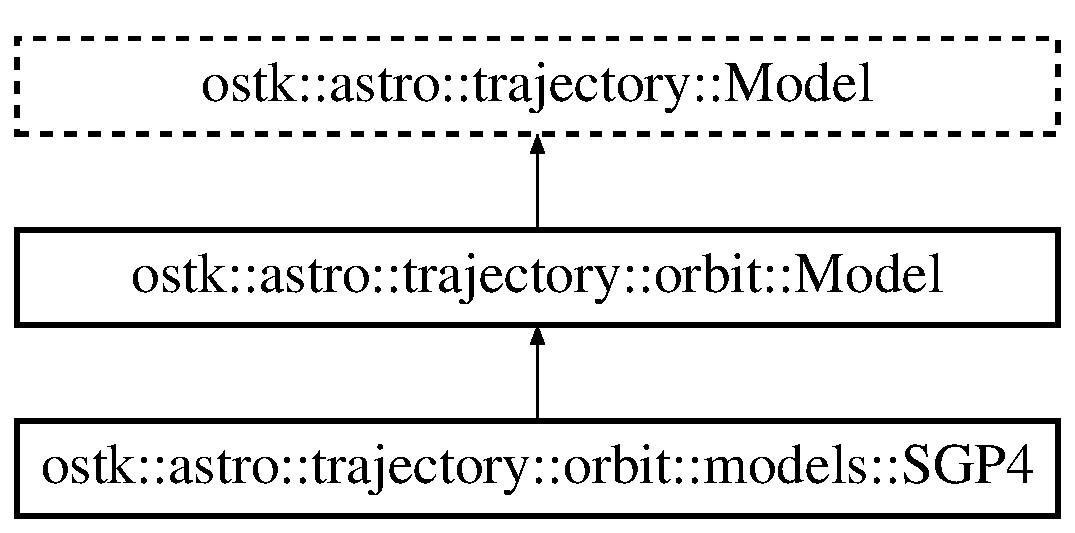
\includegraphics[height=3.000000cm]{classostk_1_1astro_1_1trajectory_1_1orbit_1_1models_1_1_s_g_p4}
\end{center}
\end{figure}
\subsection*{Public Member Functions}
\begin{DoxyCompactItemize}
\item 
\hyperlink{classostk_1_1astro_1_1trajectory_1_1orbit_1_1models_1_1_s_g_p4_a84e2bc60fdf9b295e0ab8a42ecfb51ff}{S\+G\+P4} (const \hyperlink{classostk_1_1astro_1_1trajectory_1_1orbit_1_1models_1_1sgp4_1_1_t_l_e}{T\+LE} \&a\+Tle)
\item 
\hyperlink{classostk_1_1astro_1_1trajectory_1_1orbit_1_1models_1_1_s_g_p4_afe0c5fa943d25263097c242c5b289239}{S\+G\+P4} (const \hyperlink{classostk_1_1astro_1_1trajectory_1_1orbit_1_1models_1_1_s_g_p4}{S\+G\+P4} \&a\+S\+G\+P4\+Model)
\item 
\hyperlink{classostk_1_1astro_1_1trajectory_1_1orbit_1_1models_1_1_s_g_p4_a00ac84881288a79f3c876efd56c376eb}{$\sim$\+S\+G\+P4} ()
\item 
\hyperlink{classostk_1_1astro_1_1trajectory_1_1orbit_1_1models_1_1_s_g_p4}{S\+G\+P4} \& \hyperlink{classostk_1_1astro_1_1trajectory_1_1orbit_1_1models_1_1_s_g_p4_a8f8d3633270de5c9d8c99f047f28d0f0}{operator=} (const \hyperlink{classostk_1_1astro_1_1trajectory_1_1orbit_1_1models_1_1_s_g_p4}{S\+G\+P4} \&a\+S\+G\+P4\+Model)
\item 
virtual \hyperlink{classostk_1_1astro_1_1trajectory_1_1orbit_1_1models_1_1_s_g_p4}{S\+G\+P4} $\ast$ \hyperlink{classostk_1_1astro_1_1trajectory_1_1orbit_1_1models_1_1_s_g_p4_afb9928e09d66c13a77eb1126da6139eb}{clone} () const override
\item 
bool \hyperlink{classostk_1_1astro_1_1trajectory_1_1orbit_1_1models_1_1_s_g_p4_ac95f88e801e75d53c2908cfc55d743a0}{operator==} (const \hyperlink{classostk_1_1astro_1_1trajectory_1_1orbit_1_1models_1_1_s_g_p4}{S\+G\+P4} \&a\+S\+G\+P4\+Model) const
\item 
bool \hyperlink{classostk_1_1astro_1_1trajectory_1_1orbit_1_1models_1_1_s_g_p4_a6daa973c340543e56c134cd2daf867f6}{operator!=} (const \hyperlink{classostk_1_1astro_1_1trajectory_1_1orbit_1_1models_1_1_s_g_p4}{S\+G\+P4} \&a\+S\+G\+P4\+Model) const
\item 
virtual bool \hyperlink{classostk_1_1astro_1_1trajectory_1_1orbit_1_1models_1_1_s_g_p4_ab18e0666588bd517c190942b1a54ed18}{is\+Defined} () const override
\item 
\hyperlink{classostk_1_1astro_1_1trajectory_1_1orbit_1_1models_1_1sgp4_1_1_t_l_e}{T\+LE} \hyperlink{classostk_1_1astro_1_1trajectory_1_1orbit_1_1models_1_1_s_g_p4_ac1f2188866759569091ebfd8e43919a8}{get\+Tle} () const
\item 
virtual Instant \hyperlink{classostk_1_1astro_1_1trajectory_1_1orbit_1_1models_1_1_s_g_p4_af577ee4ad56452fe510d325a61a9792e}{get\+Epoch} () const override
\item 
virtual Integer \hyperlink{classostk_1_1astro_1_1trajectory_1_1orbit_1_1models_1_1_s_g_p4_a6216f01c1ee37817ca1ae1c7036f942c}{get\+Revolution\+Number\+At\+Epoch} () const override
\item 
virtual \hyperlink{classostk_1_1astro_1_1trajectory_1_1_state}{State} \hyperlink{classostk_1_1astro_1_1trajectory_1_1orbit_1_1models_1_1_s_g_p4_ad88439d9c46a75d3da8c20d2872271e3}{calculate\+State\+At} (const Instant \&an\+Instant) const override
\item 
virtual Integer \hyperlink{classostk_1_1astro_1_1trajectory_1_1orbit_1_1models_1_1_s_g_p4_af14e7851024d96eb20033ca9296dc003}{calculate\+Revolution\+Number\+At} (const Instant \&an\+Instant) const override
\item 
virtual void \hyperlink{classostk_1_1astro_1_1trajectory_1_1orbit_1_1models_1_1_s_g_p4_a12416476201382c3d1e3c620f7be106a}{print} (std\+::ostream \&an\+Output\+Stream, bool display\+Decorator=true) const override
\end{DoxyCompactItemize}
\subsection*{Protected Member Functions}
\begin{DoxyCompactItemize}
\item 
virtual bool \hyperlink{classostk_1_1astro_1_1trajectory_1_1orbit_1_1models_1_1_s_g_p4_ad51d979b8b9b37251b6381cfe9df55ea}{operator==} (const \hyperlink{classostk_1_1astro_1_1trajectory_1_1_model}{trajectory\+::\+Model} \&a\+Model) const override
\item 
virtual bool \hyperlink{classostk_1_1astro_1_1trajectory_1_1orbit_1_1models_1_1_s_g_p4_a87441104e4e1c63356abe0632b56edb6}{operator!=} (const \hyperlink{classostk_1_1astro_1_1trajectory_1_1_model}{trajectory\+::\+Model} \&a\+Model) const override
\end{DoxyCompactItemize}
\subsection*{Friends}
\begin{DoxyCompactItemize}
\item 
std\+::ostream \& \hyperlink{classostk_1_1astro_1_1trajectory_1_1orbit_1_1models_1_1_s_g_p4_a44bd6a41f5d1be384d07b897785529f1}{operator$<$$<$} (std\+::ostream \&an\+Output\+Stream, const \hyperlink{classostk_1_1astro_1_1trajectory_1_1orbit_1_1models_1_1_s_g_p4}{S\+G\+P4} \&a\+S\+G\+P4\+Model)
\end{DoxyCompactItemize}


\subsection{Constructor \& Destructor Documentation}
\mbox{\Hypertarget{classostk_1_1astro_1_1trajectory_1_1orbit_1_1models_1_1_s_g_p4_a84e2bc60fdf9b295e0ab8a42ecfb51ff}\label{classostk_1_1astro_1_1trajectory_1_1orbit_1_1models_1_1_s_g_p4_a84e2bc60fdf9b295e0ab8a42ecfb51ff}} 
\index{ostk\+::astro\+::trajectory\+::orbit\+::models\+::\+S\+G\+P4@{ostk\+::astro\+::trajectory\+::orbit\+::models\+::\+S\+G\+P4}!S\+G\+P4@{S\+G\+P4}}
\index{S\+G\+P4@{S\+G\+P4}!ostk\+::astro\+::trajectory\+::orbit\+::models\+::\+S\+G\+P4@{ostk\+::astro\+::trajectory\+::orbit\+::models\+::\+S\+G\+P4}}
\subsubsection{\texorpdfstring{S\+G\+P4()}{SGP4()}\hspace{0.1cm}{\footnotesize\ttfamily [1/2]}}
{\footnotesize\ttfamily ostk\+::astro\+::trajectory\+::orbit\+::models\+::\+S\+G\+P4\+::\+S\+G\+P4 (\begin{DoxyParamCaption}\item[{const \hyperlink{classostk_1_1astro_1_1trajectory_1_1orbit_1_1models_1_1sgp4_1_1_t_l_e}{T\+LE} \&}]{a\+Tle }\end{DoxyParamCaption})}

\mbox{\Hypertarget{classostk_1_1astro_1_1trajectory_1_1orbit_1_1models_1_1_s_g_p4_afe0c5fa943d25263097c242c5b289239}\label{classostk_1_1astro_1_1trajectory_1_1orbit_1_1models_1_1_s_g_p4_afe0c5fa943d25263097c242c5b289239}} 
\index{ostk\+::astro\+::trajectory\+::orbit\+::models\+::\+S\+G\+P4@{ostk\+::astro\+::trajectory\+::orbit\+::models\+::\+S\+G\+P4}!S\+G\+P4@{S\+G\+P4}}
\index{S\+G\+P4@{S\+G\+P4}!ostk\+::astro\+::trajectory\+::orbit\+::models\+::\+S\+G\+P4@{ostk\+::astro\+::trajectory\+::orbit\+::models\+::\+S\+G\+P4}}
\subsubsection{\texorpdfstring{S\+G\+P4()}{SGP4()}\hspace{0.1cm}{\footnotesize\ttfamily [2/2]}}
{\footnotesize\ttfamily ostk\+::astro\+::trajectory\+::orbit\+::models\+::\+S\+G\+P4\+::\+S\+G\+P4 (\begin{DoxyParamCaption}\item[{const \hyperlink{classostk_1_1astro_1_1trajectory_1_1orbit_1_1models_1_1_s_g_p4}{S\+G\+P4} \&}]{a\+S\+G\+P4\+Model }\end{DoxyParamCaption})}

\mbox{\Hypertarget{classostk_1_1astro_1_1trajectory_1_1orbit_1_1models_1_1_s_g_p4_a00ac84881288a79f3c876efd56c376eb}\label{classostk_1_1astro_1_1trajectory_1_1orbit_1_1models_1_1_s_g_p4_a00ac84881288a79f3c876efd56c376eb}} 
\index{ostk\+::astro\+::trajectory\+::orbit\+::models\+::\+S\+G\+P4@{ostk\+::astro\+::trajectory\+::orbit\+::models\+::\+S\+G\+P4}!````~S\+G\+P4@{$\sim$\+S\+G\+P4}}
\index{````~S\+G\+P4@{$\sim$\+S\+G\+P4}!ostk\+::astro\+::trajectory\+::orbit\+::models\+::\+S\+G\+P4@{ostk\+::astro\+::trajectory\+::orbit\+::models\+::\+S\+G\+P4}}
\subsubsection{\texorpdfstring{$\sim$\+S\+G\+P4()}{~SGP4()}}
{\footnotesize\ttfamily ostk\+::astro\+::trajectory\+::orbit\+::models\+::\+S\+G\+P4\+::$\sim$\+S\+G\+P4 (\begin{DoxyParamCaption}{ }\end{DoxyParamCaption})}



\subsection{Member Function Documentation}
\mbox{\Hypertarget{classostk_1_1astro_1_1trajectory_1_1orbit_1_1models_1_1_s_g_p4_af14e7851024d96eb20033ca9296dc003}\label{classostk_1_1astro_1_1trajectory_1_1orbit_1_1models_1_1_s_g_p4_af14e7851024d96eb20033ca9296dc003}} 
\index{ostk\+::astro\+::trajectory\+::orbit\+::models\+::\+S\+G\+P4@{ostk\+::astro\+::trajectory\+::orbit\+::models\+::\+S\+G\+P4}!calculate\+Revolution\+Number\+At@{calculate\+Revolution\+Number\+At}}
\index{calculate\+Revolution\+Number\+At@{calculate\+Revolution\+Number\+At}!ostk\+::astro\+::trajectory\+::orbit\+::models\+::\+S\+G\+P4@{ostk\+::astro\+::trajectory\+::orbit\+::models\+::\+S\+G\+P4}}
\subsubsection{\texorpdfstring{calculate\+Revolution\+Number\+At()}{calculateRevolutionNumberAt()}}
{\footnotesize\ttfamily Integer ostk\+::astro\+::trajectory\+::orbit\+::models\+::\+S\+G\+P4\+::calculate\+Revolution\+Number\+At (\begin{DoxyParamCaption}\item[{const Instant \&}]{an\+Instant }\end{DoxyParamCaption}) const\hspace{0.3cm}{\ttfamily [override]}, {\ttfamily [virtual]}}



Implements \hyperlink{classostk_1_1astro_1_1trajectory_1_1orbit_1_1_model_aeecf4cc22fa9c766801936c468cc52ac}{ostk\+::astro\+::trajectory\+::orbit\+::\+Model}.

\mbox{\Hypertarget{classostk_1_1astro_1_1trajectory_1_1orbit_1_1models_1_1_s_g_p4_ad88439d9c46a75d3da8c20d2872271e3}\label{classostk_1_1astro_1_1trajectory_1_1orbit_1_1models_1_1_s_g_p4_ad88439d9c46a75d3da8c20d2872271e3}} 
\index{ostk\+::astro\+::trajectory\+::orbit\+::models\+::\+S\+G\+P4@{ostk\+::astro\+::trajectory\+::orbit\+::models\+::\+S\+G\+P4}!calculate\+State\+At@{calculate\+State\+At}}
\index{calculate\+State\+At@{calculate\+State\+At}!ostk\+::astro\+::trajectory\+::orbit\+::models\+::\+S\+G\+P4@{ostk\+::astro\+::trajectory\+::orbit\+::models\+::\+S\+G\+P4}}
\subsubsection{\texorpdfstring{calculate\+State\+At()}{calculateStateAt()}}
{\footnotesize\ttfamily \hyperlink{classostk_1_1astro_1_1trajectory_1_1_state}{State} ostk\+::astro\+::trajectory\+::orbit\+::models\+::\+S\+G\+P4\+::calculate\+State\+At (\begin{DoxyParamCaption}\item[{const Instant \&}]{an\+Instant }\end{DoxyParamCaption}) const\hspace{0.3cm}{\ttfamily [override]}, {\ttfamily [virtual]}}



Implements \hyperlink{classostk_1_1astro_1_1trajectory_1_1orbit_1_1_model_a34a0d8979ec1f7ade3e434fc0dad3711}{ostk\+::astro\+::trajectory\+::orbit\+::\+Model}.

\mbox{\Hypertarget{classostk_1_1astro_1_1trajectory_1_1orbit_1_1models_1_1_s_g_p4_afb9928e09d66c13a77eb1126da6139eb}\label{classostk_1_1astro_1_1trajectory_1_1orbit_1_1models_1_1_s_g_p4_afb9928e09d66c13a77eb1126da6139eb}} 
\index{ostk\+::astro\+::trajectory\+::orbit\+::models\+::\+S\+G\+P4@{ostk\+::astro\+::trajectory\+::orbit\+::models\+::\+S\+G\+P4}!clone@{clone}}
\index{clone@{clone}!ostk\+::astro\+::trajectory\+::orbit\+::models\+::\+S\+G\+P4@{ostk\+::astro\+::trajectory\+::orbit\+::models\+::\+S\+G\+P4}}
\subsubsection{\texorpdfstring{clone()}{clone()}}
{\footnotesize\ttfamily \hyperlink{classostk_1_1astro_1_1trajectory_1_1orbit_1_1models_1_1_s_g_p4}{S\+G\+P4} $\ast$ ostk\+::astro\+::trajectory\+::orbit\+::models\+::\+S\+G\+P4\+::clone (\begin{DoxyParamCaption}{ }\end{DoxyParamCaption}) const\hspace{0.3cm}{\ttfamily [override]}, {\ttfamily [virtual]}}



Implements \hyperlink{classostk_1_1astro_1_1trajectory_1_1orbit_1_1_model_a53dc07564e4c7c444da46360aa8ada15}{ostk\+::astro\+::trajectory\+::orbit\+::\+Model}.

\mbox{\Hypertarget{classostk_1_1astro_1_1trajectory_1_1orbit_1_1models_1_1_s_g_p4_af577ee4ad56452fe510d325a61a9792e}\label{classostk_1_1astro_1_1trajectory_1_1orbit_1_1models_1_1_s_g_p4_af577ee4ad56452fe510d325a61a9792e}} 
\index{ostk\+::astro\+::trajectory\+::orbit\+::models\+::\+S\+G\+P4@{ostk\+::astro\+::trajectory\+::orbit\+::models\+::\+S\+G\+P4}!get\+Epoch@{get\+Epoch}}
\index{get\+Epoch@{get\+Epoch}!ostk\+::astro\+::trajectory\+::orbit\+::models\+::\+S\+G\+P4@{ostk\+::astro\+::trajectory\+::orbit\+::models\+::\+S\+G\+P4}}
\subsubsection{\texorpdfstring{get\+Epoch()}{getEpoch()}}
{\footnotesize\ttfamily Instant ostk\+::astro\+::trajectory\+::orbit\+::models\+::\+S\+G\+P4\+::get\+Epoch (\begin{DoxyParamCaption}{ }\end{DoxyParamCaption}) const\hspace{0.3cm}{\ttfamily [override]}, {\ttfamily [virtual]}}



Implements \hyperlink{classostk_1_1astro_1_1trajectory_1_1orbit_1_1_model_a22055d5ab4c22e6177a3ddb8f45f1f9b}{ostk\+::astro\+::trajectory\+::orbit\+::\+Model}.

\mbox{\Hypertarget{classostk_1_1astro_1_1trajectory_1_1orbit_1_1models_1_1_s_g_p4_a6216f01c1ee37817ca1ae1c7036f942c}\label{classostk_1_1astro_1_1trajectory_1_1orbit_1_1models_1_1_s_g_p4_a6216f01c1ee37817ca1ae1c7036f942c}} 
\index{ostk\+::astro\+::trajectory\+::orbit\+::models\+::\+S\+G\+P4@{ostk\+::astro\+::trajectory\+::orbit\+::models\+::\+S\+G\+P4}!get\+Revolution\+Number\+At\+Epoch@{get\+Revolution\+Number\+At\+Epoch}}
\index{get\+Revolution\+Number\+At\+Epoch@{get\+Revolution\+Number\+At\+Epoch}!ostk\+::astro\+::trajectory\+::orbit\+::models\+::\+S\+G\+P4@{ostk\+::astro\+::trajectory\+::orbit\+::models\+::\+S\+G\+P4}}
\subsubsection{\texorpdfstring{get\+Revolution\+Number\+At\+Epoch()}{getRevolutionNumberAtEpoch()}}
{\footnotesize\ttfamily Integer ostk\+::astro\+::trajectory\+::orbit\+::models\+::\+S\+G\+P4\+::get\+Revolution\+Number\+At\+Epoch (\begin{DoxyParamCaption}{ }\end{DoxyParamCaption}) const\hspace{0.3cm}{\ttfamily [override]}, {\ttfamily [virtual]}}



Implements \hyperlink{classostk_1_1astro_1_1trajectory_1_1orbit_1_1_model_af3f1866f86045da2c05efe4165735cf4}{ostk\+::astro\+::trajectory\+::orbit\+::\+Model}.

\mbox{\Hypertarget{classostk_1_1astro_1_1trajectory_1_1orbit_1_1models_1_1_s_g_p4_ac1f2188866759569091ebfd8e43919a8}\label{classostk_1_1astro_1_1trajectory_1_1orbit_1_1models_1_1_s_g_p4_ac1f2188866759569091ebfd8e43919a8}} 
\index{ostk\+::astro\+::trajectory\+::orbit\+::models\+::\+S\+G\+P4@{ostk\+::astro\+::trajectory\+::orbit\+::models\+::\+S\+G\+P4}!get\+Tle@{get\+Tle}}
\index{get\+Tle@{get\+Tle}!ostk\+::astro\+::trajectory\+::orbit\+::models\+::\+S\+G\+P4@{ostk\+::astro\+::trajectory\+::orbit\+::models\+::\+S\+G\+P4}}
\subsubsection{\texorpdfstring{get\+Tle()}{getTle()}}
{\footnotesize\ttfamily \hyperlink{classostk_1_1astro_1_1trajectory_1_1orbit_1_1models_1_1sgp4_1_1_t_l_e}{T\+LE} ostk\+::astro\+::trajectory\+::orbit\+::models\+::\+S\+G\+P4\+::get\+Tle (\begin{DoxyParamCaption}{ }\end{DoxyParamCaption}) const}

\mbox{\Hypertarget{classostk_1_1astro_1_1trajectory_1_1orbit_1_1models_1_1_s_g_p4_ab18e0666588bd517c190942b1a54ed18}\label{classostk_1_1astro_1_1trajectory_1_1orbit_1_1models_1_1_s_g_p4_ab18e0666588bd517c190942b1a54ed18}} 
\index{ostk\+::astro\+::trajectory\+::orbit\+::models\+::\+S\+G\+P4@{ostk\+::astro\+::trajectory\+::orbit\+::models\+::\+S\+G\+P4}!is\+Defined@{is\+Defined}}
\index{is\+Defined@{is\+Defined}!ostk\+::astro\+::trajectory\+::orbit\+::models\+::\+S\+G\+P4@{ostk\+::astro\+::trajectory\+::orbit\+::models\+::\+S\+G\+P4}}
\subsubsection{\texorpdfstring{is\+Defined()}{isDefined()}}
{\footnotesize\ttfamily bool ostk\+::astro\+::trajectory\+::orbit\+::models\+::\+S\+G\+P4\+::is\+Defined (\begin{DoxyParamCaption}{ }\end{DoxyParamCaption}) const\hspace{0.3cm}{\ttfamily [override]}, {\ttfamily [virtual]}}



Implements \hyperlink{classostk_1_1astro_1_1trajectory_1_1orbit_1_1_model_a13c5b5693dd86a072da0bd0e319bacc2}{ostk\+::astro\+::trajectory\+::orbit\+::\+Model}.

\mbox{\Hypertarget{classostk_1_1astro_1_1trajectory_1_1orbit_1_1models_1_1_s_g_p4_a6daa973c340543e56c134cd2daf867f6}\label{classostk_1_1astro_1_1trajectory_1_1orbit_1_1models_1_1_s_g_p4_a6daa973c340543e56c134cd2daf867f6}} 
\index{ostk\+::astro\+::trajectory\+::orbit\+::models\+::\+S\+G\+P4@{ostk\+::astro\+::trajectory\+::orbit\+::models\+::\+S\+G\+P4}!operator"!=@{operator"!=}}
\index{operator"!=@{operator"!=}!ostk\+::astro\+::trajectory\+::orbit\+::models\+::\+S\+G\+P4@{ostk\+::astro\+::trajectory\+::orbit\+::models\+::\+S\+G\+P4}}
\subsubsection{\texorpdfstring{operator"!=()}{operator!=()}\hspace{0.1cm}{\footnotesize\ttfamily [1/2]}}
{\footnotesize\ttfamily bool ostk\+::astro\+::trajectory\+::orbit\+::models\+::\+S\+G\+P4\+::operator!= (\begin{DoxyParamCaption}\item[{const \hyperlink{classostk_1_1astro_1_1trajectory_1_1orbit_1_1models_1_1_s_g_p4}{S\+G\+P4} \&}]{a\+S\+G\+P4\+Model }\end{DoxyParamCaption}) const}

\mbox{\Hypertarget{classostk_1_1astro_1_1trajectory_1_1orbit_1_1models_1_1_s_g_p4_a87441104e4e1c63356abe0632b56edb6}\label{classostk_1_1astro_1_1trajectory_1_1orbit_1_1models_1_1_s_g_p4_a87441104e4e1c63356abe0632b56edb6}} 
\index{ostk\+::astro\+::trajectory\+::orbit\+::models\+::\+S\+G\+P4@{ostk\+::astro\+::trajectory\+::orbit\+::models\+::\+S\+G\+P4}!operator"!=@{operator"!=}}
\index{operator"!=@{operator"!=}!ostk\+::astro\+::trajectory\+::orbit\+::models\+::\+S\+G\+P4@{ostk\+::astro\+::trajectory\+::orbit\+::models\+::\+S\+G\+P4}}
\subsubsection{\texorpdfstring{operator"!=()}{operator!=()}\hspace{0.1cm}{\footnotesize\ttfamily [2/2]}}
{\footnotesize\ttfamily bool ostk\+::astro\+::trajectory\+::orbit\+::models\+::\+S\+G\+P4\+::operator!= (\begin{DoxyParamCaption}\item[{const \hyperlink{classostk_1_1astro_1_1trajectory_1_1_model}{trajectory\+::\+Model} \&}]{a\+Model }\end{DoxyParamCaption}) const\hspace{0.3cm}{\ttfamily [override]}, {\ttfamily [protected]}, {\ttfamily [virtual]}}



Implements \hyperlink{classostk_1_1astro_1_1trajectory_1_1_model_a2dd77b9f6939d738f3a489f26c955340}{ostk\+::astro\+::trajectory\+::\+Model}.

\mbox{\Hypertarget{classostk_1_1astro_1_1trajectory_1_1orbit_1_1models_1_1_s_g_p4_a8f8d3633270de5c9d8c99f047f28d0f0}\label{classostk_1_1astro_1_1trajectory_1_1orbit_1_1models_1_1_s_g_p4_a8f8d3633270de5c9d8c99f047f28d0f0}} 
\index{ostk\+::astro\+::trajectory\+::orbit\+::models\+::\+S\+G\+P4@{ostk\+::astro\+::trajectory\+::orbit\+::models\+::\+S\+G\+P4}!operator=@{operator=}}
\index{operator=@{operator=}!ostk\+::astro\+::trajectory\+::orbit\+::models\+::\+S\+G\+P4@{ostk\+::astro\+::trajectory\+::orbit\+::models\+::\+S\+G\+P4}}
\subsubsection{\texorpdfstring{operator=()}{operator=()}}
{\footnotesize\ttfamily \hyperlink{classostk_1_1astro_1_1trajectory_1_1orbit_1_1models_1_1_s_g_p4}{S\+G\+P4} \& ostk\+::astro\+::trajectory\+::orbit\+::models\+::\+S\+G\+P4\+::operator= (\begin{DoxyParamCaption}\item[{const \hyperlink{classostk_1_1astro_1_1trajectory_1_1orbit_1_1models_1_1_s_g_p4}{S\+G\+P4} \&}]{a\+S\+G\+P4\+Model }\end{DoxyParamCaption})}

\mbox{\Hypertarget{classostk_1_1astro_1_1trajectory_1_1orbit_1_1models_1_1_s_g_p4_ac95f88e801e75d53c2908cfc55d743a0}\label{classostk_1_1astro_1_1trajectory_1_1orbit_1_1models_1_1_s_g_p4_ac95f88e801e75d53c2908cfc55d743a0}} 
\index{ostk\+::astro\+::trajectory\+::orbit\+::models\+::\+S\+G\+P4@{ostk\+::astro\+::trajectory\+::orbit\+::models\+::\+S\+G\+P4}!operator==@{operator==}}
\index{operator==@{operator==}!ostk\+::astro\+::trajectory\+::orbit\+::models\+::\+S\+G\+P4@{ostk\+::astro\+::trajectory\+::orbit\+::models\+::\+S\+G\+P4}}
\subsubsection{\texorpdfstring{operator==()}{operator==()}\hspace{0.1cm}{\footnotesize\ttfamily [1/2]}}
{\footnotesize\ttfamily bool ostk\+::astro\+::trajectory\+::orbit\+::models\+::\+S\+G\+P4\+::operator== (\begin{DoxyParamCaption}\item[{const \hyperlink{classostk_1_1astro_1_1trajectory_1_1orbit_1_1models_1_1_s_g_p4}{S\+G\+P4} \&}]{a\+S\+G\+P4\+Model }\end{DoxyParamCaption}) const}

\mbox{\Hypertarget{classostk_1_1astro_1_1trajectory_1_1orbit_1_1models_1_1_s_g_p4_ad51d979b8b9b37251b6381cfe9df55ea}\label{classostk_1_1astro_1_1trajectory_1_1orbit_1_1models_1_1_s_g_p4_ad51d979b8b9b37251b6381cfe9df55ea}} 
\index{ostk\+::astro\+::trajectory\+::orbit\+::models\+::\+S\+G\+P4@{ostk\+::astro\+::trajectory\+::orbit\+::models\+::\+S\+G\+P4}!operator==@{operator==}}
\index{operator==@{operator==}!ostk\+::astro\+::trajectory\+::orbit\+::models\+::\+S\+G\+P4@{ostk\+::astro\+::trajectory\+::orbit\+::models\+::\+S\+G\+P4}}
\subsubsection{\texorpdfstring{operator==()}{operator==()}\hspace{0.1cm}{\footnotesize\ttfamily [2/2]}}
{\footnotesize\ttfamily bool ostk\+::astro\+::trajectory\+::orbit\+::models\+::\+S\+G\+P4\+::operator== (\begin{DoxyParamCaption}\item[{const \hyperlink{classostk_1_1astro_1_1trajectory_1_1_model}{trajectory\+::\+Model} \&}]{a\+Model }\end{DoxyParamCaption}) const\hspace{0.3cm}{\ttfamily [override]}, {\ttfamily [protected]}, {\ttfamily [virtual]}}



Implements \hyperlink{classostk_1_1astro_1_1trajectory_1_1_model_a874f79846e845859c070ce1b9874fc9c}{ostk\+::astro\+::trajectory\+::\+Model}.

\mbox{\Hypertarget{classostk_1_1astro_1_1trajectory_1_1orbit_1_1models_1_1_s_g_p4_a12416476201382c3d1e3c620f7be106a}\label{classostk_1_1astro_1_1trajectory_1_1orbit_1_1models_1_1_s_g_p4_a12416476201382c3d1e3c620f7be106a}} 
\index{ostk\+::astro\+::trajectory\+::orbit\+::models\+::\+S\+G\+P4@{ostk\+::astro\+::trajectory\+::orbit\+::models\+::\+S\+G\+P4}!print@{print}}
\index{print@{print}!ostk\+::astro\+::trajectory\+::orbit\+::models\+::\+S\+G\+P4@{ostk\+::astro\+::trajectory\+::orbit\+::models\+::\+S\+G\+P4}}
\subsubsection{\texorpdfstring{print()}{print()}}
{\footnotesize\ttfamily void ostk\+::astro\+::trajectory\+::orbit\+::models\+::\+S\+G\+P4\+::print (\begin{DoxyParamCaption}\item[{std\+::ostream \&}]{an\+Output\+Stream,  }\item[{bool}]{display\+Decorator = {\ttfamily true} }\end{DoxyParamCaption}) const\hspace{0.3cm}{\ttfamily [override]}, {\ttfamily [virtual]}}



Implements \hyperlink{classostk_1_1astro_1_1trajectory_1_1orbit_1_1_model_a8ea45c1a6e51a6153ce3f72f5294f0c6}{ostk\+::astro\+::trajectory\+::orbit\+::\+Model}.



\subsection{Friends And Related Function Documentation}
\mbox{\Hypertarget{classostk_1_1astro_1_1trajectory_1_1orbit_1_1models_1_1_s_g_p4_a44bd6a41f5d1be384d07b897785529f1}\label{classostk_1_1astro_1_1trajectory_1_1orbit_1_1models_1_1_s_g_p4_a44bd6a41f5d1be384d07b897785529f1}} 
\index{ostk\+::astro\+::trajectory\+::orbit\+::models\+::\+S\+G\+P4@{ostk\+::astro\+::trajectory\+::orbit\+::models\+::\+S\+G\+P4}!operator$<$$<$@{operator$<$$<$}}
\index{operator$<$$<$@{operator$<$$<$}!ostk\+::astro\+::trajectory\+::orbit\+::models\+::\+S\+G\+P4@{ostk\+::astro\+::trajectory\+::orbit\+::models\+::\+S\+G\+P4}}
\subsubsection{\texorpdfstring{operator$<$$<$}{operator<<}}
{\footnotesize\ttfamily std\+::ostream\& operator$<$$<$ (\begin{DoxyParamCaption}\item[{std\+::ostream \&}]{an\+Output\+Stream,  }\item[{const \hyperlink{classostk_1_1astro_1_1trajectory_1_1orbit_1_1models_1_1_s_g_p4}{S\+G\+P4} \&}]{a\+S\+G\+P4\+Model }\end{DoxyParamCaption})\hspace{0.3cm}{\ttfamily [friend]}}



The documentation for this class was generated from the following files\+:\begin{DoxyCompactItemize}
\item 
include/\+Open\+Space\+Toolkit/\+Astrodynamics/\+Trajectory/\+Orbit/\+Models/\hyperlink{_s_g_p4_8hpp}{S\+G\+P4.\+hpp}\item 
src/\+Open\+Space\+Toolkit/\+Astrodynamics/\+Trajectory/\+Orbit/\+Models/\hyperlink{_s_g_p4_8cpp}{S\+G\+P4.\+cpp}\end{DoxyCompactItemize}

\hypertarget{classostk_1_1astro_1_1trajectory_1_1_state}{}\section{ostk\+:\+:astro\+:\+:trajectory\+:\+:State Class Reference}
\label{classostk_1_1astro_1_1trajectory_1_1_state}\index{ostk\+::astro\+::trajectory\+::\+State@{ostk\+::astro\+::trajectory\+::\+State}}


\hyperlink{classostk_1_1astro_1_1_trajectory}{Trajectory} state.  




{\ttfamily \#include $<$State.\+hpp$>$}

\subsection*{Public Member Functions}
\begin{DoxyCompactItemize}
\item 
\hyperlink{classostk_1_1astro_1_1trajectory_1_1_state_a8628aceae903c9492f0fb269888434b0}{State} (const Instant \&an\+Instant, const Position \&a\+Position, const Velocity \&a\+Velocity)
\item 
bool \hyperlink{classostk_1_1astro_1_1trajectory_1_1_state_acd68798b63a7e3a89e61b4b668d8dbb0}{operator==} (const \hyperlink{classostk_1_1astro_1_1trajectory_1_1_state}{State} \&a\+State) const
\item 
bool \hyperlink{classostk_1_1astro_1_1trajectory_1_1_state_a53ac2b13092bc7777efa14362fec4c46}{operator!=} (const \hyperlink{classostk_1_1astro_1_1trajectory_1_1_state}{State} \&a\+State) const
\item 
\hyperlink{classostk_1_1astro_1_1trajectory_1_1_state}{State} \hyperlink{classostk_1_1astro_1_1trajectory_1_1_state_a8d8ff34816c5e4895f9274fc06dbb799}{operator+} (const \hyperlink{classostk_1_1astro_1_1trajectory_1_1_state}{State} \&a\+State) const
\item 
\hyperlink{classostk_1_1astro_1_1trajectory_1_1_state}{State} \hyperlink{classostk_1_1astro_1_1trajectory_1_1_state_abd0979467d66ca07b86d5405255d26ed}{operator-\/} (const \hyperlink{classostk_1_1astro_1_1trajectory_1_1_state}{State} \&a\+State) const
\item 
bool \hyperlink{classostk_1_1astro_1_1trajectory_1_1_state_a09966efb00e3206cc2d20935c55658ad}{is\+Defined} () const
\item 
const Instant \& \hyperlink{classostk_1_1astro_1_1trajectory_1_1_state_afc21870411eef52ce1293e31eda16d3c}{access\+Instant} () const
\item 
const Position \& \hyperlink{classostk_1_1astro_1_1trajectory_1_1_state_a711322a78c02f981d11ebec2ca0a0cd4}{access\+Position} () const
\item 
const Velocity \& \hyperlink{classostk_1_1astro_1_1trajectory_1_1_state_a7f6d626b9d5f045e026cd1ff2ea33200}{access\+Velocity} () const
\item 
Instant \hyperlink{classostk_1_1astro_1_1trajectory_1_1_state_af1ba3040b895b0963d5fb96a0756cc2b}{get\+Instant} () const
\item 
Position \hyperlink{classostk_1_1astro_1_1trajectory_1_1_state_ad5ceac322a929f0f62214a663a21f4ae}{get\+Position} () const
\item 
Velocity \hyperlink{classostk_1_1astro_1_1trajectory_1_1_state_a1a992dcad42fb3094766907a9472e7e0}{get\+Velocity} () const
\item 
Vector\+Xd \hyperlink{classostk_1_1astro_1_1trajectory_1_1_state_adece3f2dda107d9178b40648dfbc01d0}{get\+Coordinates} () const
\item 
\hyperlink{classostk_1_1astro_1_1trajectory_1_1_state}{State} \hyperlink{classostk_1_1astro_1_1trajectory_1_1_state_aa9c95303df830f9dfed347231961dcf6}{in\+Frame} (const Shared$<$ const Frame $>$ \&a\+Frame\+S\+Ptr) const
\item 
void \hyperlink{classostk_1_1astro_1_1trajectory_1_1_state_a0072b543bbac1abe5e94609c74491b5d}{print} (std\+::ostream \&an\+Output\+Stream, bool display\+Decorator=true) const
\end{DoxyCompactItemize}
\subsection*{Static Public Member Functions}
\begin{DoxyCompactItemize}
\item 
static \hyperlink{classostk_1_1astro_1_1trajectory_1_1_state}{State} \hyperlink{classostk_1_1astro_1_1trajectory_1_1_state_ab6ed6a252eeac1d24cf3b5c65ec0c6b6}{Undefined} ()
\end{DoxyCompactItemize}
\subsection*{Friends}
\begin{DoxyCompactItemize}
\item 
std\+::ostream \& \hyperlink{classostk_1_1astro_1_1trajectory_1_1_state_abba03f039f2534d691a1dc28426e8b89}{operator$<$$<$} (std\+::ostream \&an\+Output\+Stream, const \hyperlink{classostk_1_1astro_1_1trajectory_1_1_state}{State} \&a\+State)
\end{DoxyCompactItemize}


\subsection{Detailed Description}
\hyperlink{classostk_1_1astro_1_1_trajectory}{Trajectory} state. 

\subsection{Constructor \& Destructor Documentation}
\mbox{\Hypertarget{classostk_1_1astro_1_1trajectory_1_1_state_a8628aceae903c9492f0fb269888434b0}\label{classostk_1_1astro_1_1trajectory_1_1_state_a8628aceae903c9492f0fb269888434b0}} 
\index{ostk\+::astro\+::trajectory\+::\+State@{ostk\+::astro\+::trajectory\+::\+State}!State@{State}}
\index{State@{State}!ostk\+::astro\+::trajectory\+::\+State@{ostk\+::astro\+::trajectory\+::\+State}}
\subsubsection{\texorpdfstring{State()}{State()}}
{\footnotesize\ttfamily ostk\+::astro\+::trajectory\+::\+State\+::\+State (\begin{DoxyParamCaption}\item[{const Instant \&}]{an\+Instant,  }\item[{const Position \&}]{a\+Position,  }\item[{const Velocity \&}]{a\+Velocity }\end{DoxyParamCaption})}



\subsection{Member Function Documentation}
\mbox{\Hypertarget{classostk_1_1astro_1_1trajectory_1_1_state_afc21870411eef52ce1293e31eda16d3c}\label{classostk_1_1astro_1_1trajectory_1_1_state_afc21870411eef52ce1293e31eda16d3c}} 
\index{ostk\+::astro\+::trajectory\+::\+State@{ostk\+::astro\+::trajectory\+::\+State}!access\+Instant@{access\+Instant}}
\index{access\+Instant@{access\+Instant}!ostk\+::astro\+::trajectory\+::\+State@{ostk\+::astro\+::trajectory\+::\+State}}
\subsubsection{\texorpdfstring{access\+Instant()}{accessInstant()}}
{\footnotesize\ttfamily const Instant \& ostk\+::astro\+::trajectory\+::\+State\+::access\+Instant (\begin{DoxyParamCaption}{ }\end{DoxyParamCaption}) const}

\mbox{\Hypertarget{classostk_1_1astro_1_1trajectory_1_1_state_a711322a78c02f981d11ebec2ca0a0cd4}\label{classostk_1_1astro_1_1trajectory_1_1_state_a711322a78c02f981d11ebec2ca0a0cd4}} 
\index{ostk\+::astro\+::trajectory\+::\+State@{ostk\+::astro\+::trajectory\+::\+State}!access\+Position@{access\+Position}}
\index{access\+Position@{access\+Position}!ostk\+::astro\+::trajectory\+::\+State@{ostk\+::astro\+::trajectory\+::\+State}}
\subsubsection{\texorpdfstring{access\+Position()}{accessPosition()}}
{\footnotesize\ttfamily const Position \& ostk\+::astro\+::trajectory\+::\+State\+::access\+Position (\begin{DoxyParamCaption}{ }\end{DoxyParamCaption}) const}

\mbox{\Hypertarget{classostk_1_1astro_1_1trajectory_1_1_state_a7f6d626b9d5f045e026cd1ff2ea33200}\label{classostk_1_1astro_1_1trajectory_1_1_state_a7f6d626b9d5f045e026cd1ff2ea33200}} 
\index{ostk\+::astro\+::trajectory\+::\+State@{ostk\+::astro\+::trajectory\+::\+State}!access\+Velocity@{access\+Velocity}}
\index{access\+Velocity@{access\+Velocity}!ostk\+::astro\+::trajectory\+::\+State@{ostk\+::astro\+::trajectory\+::\+State}}
\subsubsection{\texorpdfstring{access\+Velocity()}{accessVelocity()}}
{\footnotesize\ttfamily const Velocity \& ostk\+::astro\+::trajectory\+::\+State\+::access\+Velocity (\begin{DoxyParamCaption}{ }\end{DoxyParamCaption}) const}

\mbox{\Hypertarget{classostk_1_1astro_1_1trajectory_1_1_state_adece3f2dda107d9178b40648dfbc01d0}\label{classostk_1_1astro_1_1trajectory_1_1_state_adece3f2dda107d9178b40648dfbc01d0}} 
\index{ostk\+::astro\+::trajectory\+::\+State@{ostk\+::astro\+::trajectory\+::\+State}!get\+Coordinates@{get\+Coordinates}}
\index{get\+Coordinates@{get\+Coordinates}!ostk\+::astro\+::trajectory\+::\+State@{ostk\+::astro\+::trajectory\+::\+State}}
\subsubsection{\texorpdfstring{get\+Coordinates()}{getCoordinates()}}
{\footnotesize\ttfamily Vector\+Xd ostk\+::astro\+::trajectory\+::\+State\+::get\+Coordinates (\begin{DoxyParamCaption}{ }\end{DoxyParamCaption}) const}

\mbox{\Hypertarget{classostk_1_1astro_1_1trajectory_1_1_state_af1ba3040b895b0963d5fb96a0756cc2b}\label{classostk_1_1astro_1_1trajectory_1_1_state_af1ba3040b895b0963d5fb96a0756cc2b}} 
\index{ostk\+::astro\+::trajectory\+::\+State@{ostk\+::astro\+::trajectory\+::\+State}!get\+Instant@{get\+Instant}}
\index{get\+Instant@{get\+Instant}!ostk\+::astro\+::trajectory\+::\+State@{ostk\+::astro\+::trajectory\+::\+State}}
\subsubsection{\texorpdfstring{get\+Instant()}{getInstant()}}
{\footnotesize\ttfamily Instant ostk\+::astro\+::trajectory\+::\+State\+::get\+Instant (\begin{DoxyParamCaption}{ }\end{DoxyParamCaption}) const}

\mbox{\Hypertarget{classostk_1_1astro_1_1trajectory_1_1_state_ad5ceac322a929f0f62214a663a21f4ae}\label{classostk_1_1astro_1_1trajectory_1_1_state_ad5ceac322a929f0f62214a663a21f4ae}} 
\index{ostk\+::astro\+::trajectory\+::\+State@{ostk\+::astro\+::trajectory\+::\+State}!get\+Position@{get\+Position}}
\index{get\+Position@{get\+Position}!ostk\+::astro\+::trajectory\+::\+State@{ostk\+::astro\+::trajectory\+::\+State}}
\subsubsection{\texorpdfstring{get\+Position()}{getPosition()}}
{\footnotesize\ttfamily Position ostk\+::astro\+::trajectory\+::\+State\+::get\+Position (\begin{DoxyParamCaption}{ }\end{DoxyParamCaption}) const}

\mbox{\Hypertarget{classostk_1_1astro_1_1trajectory_1_1_state_a1a992dcad42fb3094766907a9472e7e0}\label{classostk_1_1astro_1_1trajectory_1_1_state_a1a992dcad42fb3094766907a9472e7e0}} 
\index{ostk\+::astro\+::trajectory\+::\+State@{ostk\+::astro\+::trajectory\+::\+State}!get\+Velocity@{get\+Velocity}}
\index{get\+Velocity@{get\+Velocity}!ostk\+::astro\+::trajectory\+::\+State@{ostk\+::astro\+::trajectory\+::\+State}}
\subsubsection{\texorpdfstring{get\+Velocity()}{getVelocity()}}
{\footnotesize\ttfamily Velocity ostk\+::astro\+::trajectory\+::\+State\+::get\+Velocity (\begin{DoxyParamCaption}{ }\end{DoxyParamCaption}) const}

\mbox{\Hypertarget{classostk_1_1astro_1_1trajectory_1_1_state_aa9c95303df830f9dfed347231961dcf6}\label{classostk_1_1astro_1_1trajectory_1_1_state_aa9c95303df830f9dfed347231961dcf6}} 
\index{ostk\+::astro\+::trajectory\+::\+State@{ostk\+::astro\+::trajectory\+::\+State}!in\+Frame@{in\+Frame}}
\index{in\+Frame@{in\+Frame}!ostk\+::astro\+::trajectory\+::\+State@{ostk\+::astro\+::trajectory\+::\+State}}
\subsubsection{\texorpdfstring{in\+Frame()}{inFrame()}}
{\footnotesize\ttfamily \hyperlink{classostk_1_1astro_1_1trajectory_1_1_state}{State} ostk\+::astro\+::trajectory\+::\+State\+::in\+Frame (\begin{DoxyParamCaption}\item[{const Shared$<$ const Frame $>$ \&}]{a\+Frame\+S\+Ptr }\end{DoxyParamCaption}) const}

\mbox{\Hypertarget{classostk_1_1astro_1_1trajectory_1_1_state_a09966efb00e3206cc2d20935c55658ad}\label{classostk_1_1astro_1_1trajectory_1_1_state_a09966efb00e3206cc2d20935c55658ad}} 
\index{ostk\+::astro\+::trajectory\+::\+State@{ostk\+::astro\+::trajectory\+::\+State}!is\+Defined@{is\+Defined}}
\index{is\+Defined@{is\+Defined}!ostk\+::astro\+::trajectory\+::\+State@{ostk\+::astro\+::trajectory\+::\+State}}
\subsubsection{\texorpdfstring{is\+Defined()}{isDefined()}}
{\footnotesize\ttfamily bool ostk\+::astro\+::trajectory\+::\+State\+::is\+Defined (\begin{DoxyParamCaption}{ }\end{DoxyParamCaption}) const}

\mbox{\Hypertarget{classostk_1_1astro_1_1trajectory_1_1_state_a53ac2b13092bc7777efa14362fec4c46}\label{classostk_1_1astro_1_1trajectory_1_1_state_a53ac2b13092bc7777efa14362fec4c46}} 
\index{ostk\+::astro\+::trajectory\+::\+State@{ostk\+::astro\+::trajectory\+::\+State}!operator"!=@{operator"!=}}
\index{operator"!=@{operator"!=}!ostk\+::astro\+::trajectory\+::\+State@{ostk\+::astro\+::trajectory\+::\+State}}
\subsubsection{\texorpdfstring{operator"!=()}{operator!=()}}
{\footnotesize\ttfamily bool ostk\+::astro\+::trajectory\+::\+State\+::operator!= (\begin{DoxyParamCaption}\item[{const \hyperlink{classostk_1_1astro_1_1trajectory_1_1_state}{State} \&}]{a\+State }\end{DoxyParamCaption}) const}

\mbox{\Hypertarget{classostk_1_1astro_1_1trajectory_1_1_state_a8d8ff34816c5e4895f9274fc06dbb799}\label{classostk_1_1astro_1_1trajectory_1_1_state_a8d8ff34816c5e4895f9274fc06dbb799}} 
\index{ostk\+::astro\+::trajectory\+::\+State@{ostk\+::astro\+::trajectory\+::\+State}!operator+@{operator+}}
\index{operator+@{operator+}!ostk\+::astro\+::trajectory\+::\+State@{ostk\+::astro\+::trajectory\+::\+State}}
\subsubsection{\texorpdfstring{operator+()}{operator+()}}
{\footnotesize\ttfamily \hyperlink{classostk_1_1astro_1_1trajectory_1_1_state}{State} ostk\+::astro\+::trajectory\+::\+State\+::operator+ (\begin{DoxyParamCaption}\item[{const \hyperlink{classostk_1_1astro_1_1trajectory_1_1_state}{State} \&}]{a\+State }\end{DoxyParamCaption}) const}

\mbox{\Hypertarget{classostk_1_1astro_1_1trajectory_1_1_state_abd0979467d66ca07b86d5405255d26ed}\label{classostk_1_1astro_1_1trajectory_1_1_state_abd0979467d66ca07b86d5405255d26ed}} 
\index{ostk\+::astro\+::trajectory\+::\+State@{ostk\+::astro\+::trajectory\+::\+State}!operator-\/@{operator-\/}}
\index{operator-\/@{operator-\/}!ostk\+::astro\+::trajectory\+::\+State@{ostk\+::astro\+::trajectory\+::\+State}}
\subsubsection{\texorpdfstring{operator-\/()}{operator-()}}
{\footnotesize\ttfamily \hyperlink{classostk_1_1astro_1_1trajectory_1_1_state}{State} ostk\+::astro\+::trajectory\+::\+State\+::operator-\/ (\begin{DoxyParamCaption}\item[{const \hyperlink{classostk_1_1astro_1_1trajectory_1_1_state}{State} \&}]{a\+State }\end{DoxyParamCaption}) const}

\mbox{\Hypertarget{classostk_1_1astro_1_1trajectory_1_1_state_acd68798b63a7e3a89e61b4b668d8dbb0}\label{classostk_1_1astro_1_1trajectory_1_1_state_acd68798b63a7e3a89e61b4b668d8dbb0}} 
\index{ostk\+::astro\+::trajectory\+::\+State@{ostk\+::astro\+::trajectory\+::\+State}!operator==@{operator==}}
\index{operator==@{operator==}!ostk\+::astro\+::trajectory\+::\+State@{ostk\+::astro\+::trajectory\+::\+State}}
\subsubsection{\texorpdfstring{operator==()}{operator==()}}
{\footnotesize\ttfamily bool ostk\+::astro\+::trajectory\+::\+State\+::operator== (\begin{DoxyParamCaption}\item[{const \hyperlink{classostk_1_1astro_1_1trajectory_1_1_state}{State} \&}]{a\+State }\end{DoxyParamCaption}) const}

\mbox{\Hypertarget{classostk_1_1astro_1_1trajectory_1_1_state_a0072b543bbac1abe5e94609c74491b5d}\label{classostk_1_1astro_1_1trajectory_1_1_state_a0072b543bbac1abe5e94609c74491b5d}} 
\index{ostk\+::astro\+::trajectory\+::\+State@{ostk\+::astro\+::trajectory\+::\+State}!print@{print}}
\index{print@{print}!ostk\+::astro\+::trajectory\+::\+State@{ostk\+::astro\+::trajectory\+::\+State}}
\subsubsection{\texorpdfstring{print()}{print()}}
{\footnotesize\ttfamily void ostk\+::astro\+::trajectory\+::\+State\+::print (\begin{DoxyParamCaption}\item[{std\+::ostream \&}]{an\+Output\+Stream,  }\item[{bool}]{display\+Decorator = {\ttfamily true} }\end{DoxyParamCaption}) const}

\mbox{\Hypertarget{classostk_1_1astro_1_1trajectory_1_1_state_ab6ed6a252eeac1d24cf3b5c65ec0c6b6}\label{classostk_1_1astro_1_1trajectory_1_1_state_ab6ed6a252eeac1d24cf3b5c65ec0c6b6}} 
\index{ostk\+::astro\+::trajectory\+::\+State@{ostk\+::astro\+::trajectory\+::\+State}!Undefined@{Undefined}}
\index{Undefined@{Undefined}!ostk\+::astro\+::trajectory\+::\+State@{ostk\+::astro\+::trajectory\+::\+State}}
\subsubsection{\texorpdfstring{Undefined()}{Undefined()}}
{\footnotesize\ttfamily \hyperlink{classostk_1_1astro_1_1trajectory_1_1_state}{State} ostk\+::astro\+::trajectory\+::\+State\+::\+Undefined (\begin{DoxyParamCaption}{ }\end{DoxyParamCaption})\hspace{0.3cm}{\ttfamily [static]}}



\subsection{Friends And Related Function Documentation}
\mbox{\Hypertarget{classostk_1_1astro_1_1trajectory_1_1_state_abba03f039f2534d691a1dc28426e8b89}\label{classostk_1_1astro_1_1trajectory_1_1_state_abba03f039f2534d691a1dc28426e8b89}} 
\index{ostk\+::astro\+::trajectory\+::\+State@{ostk\+::astro\+::trajectory\+::\+State}!operator$<$$<$@{operator$<$$<$}}
\index{operator$<$$<$@{operator$<$$<$}!ostk\+::astro\+::trajectory\+::\+State@{ostk\+::astro\+::trajectory\+::\+State}}
\subsubsection{\texorpdfstring{operator$<$$<$}{operator<<}}
{\footnotesize\ttfamily std\+::ostream\& operator$<$$<$ (\begin{DoxyParamCaption}\item[{std\+::ostream \&}]{an\+Output\+Stream,  }\item[{const \hyperlink{classostk_1_1astro_1_1trajectory_1_1_state}{State} \&}]{a\+State }\end{DoxyParamCaption})\hspace{0.3cm}{\ttfamily [friend]}}



The documentation for this class was generated from the following files\+:\begin{DoxyCompactItemize}
\item 
include/\+Open\+Space\+Toolkit/\+Astrodynamics/\+Trajectory/\hyperlink{_trajectory_2_state_8hpp}{State.\+hpp}\item 
src/\+Open\+Space\+Toolkit/\+Astrodynamics/\+Trajectory/\hyperlink{_trajectory_2_state_8cpp}{State.\+cpp}\end{DoxyCompactItemize}

\hypertarget{classostk_1_1astro_1_1flight_1_1profile_1_1_state}{}\section{ostk\+:\+:astro\+:\+:flight\+:\+:profile\+:\+:State Class Reference}
\label{classostk_1_1astro_1_1flight_1_1profile_1_1_state}\index{ostk\+::astro\+::flight\+::profile\+::\+State@{ostk\+::astro\+::flight\+::profile\+::\+State}}


Spacecraft flight profile state.  




{\ttfamily \#include $<$State.\+hpp$>$}

\subsection*{Public Member Functions}
\begin{DoxyCompactItemize}
\item 
\hyperlink{classostk_1_1astro_1_1flight_1_1profile_1_1_state_ac6e83efb0a774d9cbdb94c02ee17d87b}{State} (const Instant \&an\+Instant, const Vector3d \&a\+Position, const Vector3d \&a\+Velocity, const Quaternion \&an\+Attitude, const Vector3d \&an\+Angular\+Velocity, const Shared$<$ const Frame $>$ \&a\+Reference\+Frame)
\item 
bool \hyperlink{classostk_1_1astro_1_1flight_1_1profile_1_1_state_a4f6023c3c1d9590ec701bf10b0724ebf}{operator==} (const \hyperlink{classostk_1_1astro_1_1flight_1_1profile_1_1_state}{State} \&a\+State) const
\item 
bool \hyperlink{classostk_1_1astro_1_1flight_1_1profile_1_1_state_a300ff5bdda0b2bba50912f95287aba5e}{operator!=} (const \hyperlink{classostk_1_1astro_1_1flight_1_1profile_1_1_state}{State} \&a\+State) const
\item 
bool \hyperlink{classostk_1_1astro_1_1flight_1_1profile_1_1_state_ab69f291582ca4b31c9f340d9d5f83269}{is\+Defined} () const
\item 
const Instant \& \hyperlink{classostk_1_1astro_1_1flight_1_1profile_1_1_state_a6537111ca0de878dc9ccba7fbc037d41}{access\+Instant} () const
\item 
const Vector3d \& \hyperlink{classostk_1_1astro_1_1flight_1_1profile_1_1_state_a690408a5ae6d20d7812f797d20310557}{access\+Position} () const
\item 
const Vector3d \& \hyperlink{classostk_1_1astro_1_1flight_1_1profile_1_1_state_a8848af51a3b34d49f036e4a9a57231cf}{access\+Velocity} () const
\item 
const Quaternion \& \hyperlink{classostk_1_1astro_1_1flight_1_1profile_1_1_state_ad2ce6847d15311d2d1cb7a3662a1d5e4}{access\+Attitude} () const
\item 
const Vector3d \& \hyperlink{classostk_1_1astro_1_1flight_1_1profile_1_1_state_ad0118d95481db7a1bee0820aa20720af}{access\+Angular\+Velocity} () const
\item 
Instant \hyperlink{classostk_1_1astro_1_1flight_1_1profile_1_1_state_aef2c7d2c1f6831280e3933bb2d83a290}{get\+Instant} () const
\item 
Vector3d \hyperlink{classostk_1_1astro_1_1flight_1_1profile_1_1_state_ae68367f0e69fed7fc30660fc2cf98c1c}{get\+Position} () const
\item 
Vector3d \hyperlink{classostk_1_1astro_1_1flight_1_1profile_1_1_state_a6a814a57938b83db9ad8a7e13ff3ea2e}{get\+Velocity} () const
\item 
Quaternion \hyperlink{classostk_1_1astro_1_1flight_1_1profile_1_1_state_a8b765a7ebcfc0a7202bce31cafbc3a30}{get\+Attitude} () const
\item 
Vector3d \hyperlink{classostk_1_1astro_1_1flight_1_1profile_1_1_state_acd3702013017327ab64023ff86d1c3c2}{get\+Angular\+Velocity} () const
\item 
Shared$<$ const Frame $>$ \hyperlink{classostk_1_1astro_1_1flight_1_1profile_1_1_state_a6e06bfcca971466bf36c2c0a0837e429}{get\+Frame} () const
\item 
\hyperlink{classostk_1_1astro_1_1flight_1_1profile_1_1_state}{State} \hyperlink{classostk_1_1astro_1_1flight_1_1profile_1_1_state_ab5f93d12e52218cc6d5684a5a9519b87}{in\+Frame} (const Shared$<$ const Frame $>$ \&a\+Frame\+S\+Ptr) const
\end{DoxyCompactItemize}
\subsection*{Static Public Member Functions}
\begin{DoxyCompactItemize}
\item 
static \hyperlink{classostk_1_1astro_1_1flight_1_1profile_1_1_state}{State} \hyperlink{classostk_1_1astro_1_1flight_1_1profile_1_1_state_af18b40557aa14bfd0b46d14ad04d33fc}{Undefined} ()
\end{DoxyCompactItemize}
\subsection*{Friends}
\begin{DoxyCompactItemize}
\item 
std\+::ostream \& \hyperlink{classostk_1_1astro_1_1flight_1_1profile_1_1_state_abba03f039f2534d691a1dc28426e8b89}{operator$<$$<$} (std\+::ostream \&an\+Output\+Stream, const \hyperlink{classostk_1_1astro_1_1flight_1_1profile_1_1_state}{State} \&a\+State)
\end{DoxyCompactItemize}


\subsection{Detailed Description}
Spacecraft flight profile state. 

\subsection{Constructor \& Destructor Documentation}
\mbox{\Hypertarget{classostk_1_1astro_1_1flight_1_1profile_1_1_state_ac6e83efb0a774d9cbdb94c02ee17d87b}\label{classostk_1_1astro_1_1flight_1_1profile_1_1_state_ac6e83efb0a774d9cbdb94c02ee17d87b}} 
\index{ostk\+::astro\+::flight\+::profile\+::\+State@{ostk\+::astro\+::flight\+::profile\+::\+State}!State@{State}}
\index{State@{State}!ostk\+::astro\+::flight\+::profile\+::\+State@{ostk\+::astro\+::flight\+::profile\+::\+State}}
\subsubsection{\texorpdfstring{State()}{State()}}
{\footnotesize\ttfamily ostk\+::astro\+::flight\+::profile\+::\+State\+::\+State (\begin{DoxyParamCaption}\item[{const Instant \&}]{an\+Instant,  }\item[{const Vector3d \&}]{a\+Position,  }\item[{const Vector3d \&}]{a\+Velocity,  }\item[{const Quaternion \&}]{an\+Attitude,  }\item[{const Vector3d \&}]{an\+Angular\+Velocity,  }\item[{const Shared$<$ const Frame $>$ \&}]{a\+Reference\+Frame }\end{DoxyParamCaption})}



\subsection{Member Function Documentation}
\mbox{\Hypertarget{classostk_1_1astro_1_1flight_1_1profile_1_1_state_ad0118d95481db7a1bee0820aa20720af}\label{classostk_1_1astro_1_1flight_1_1profile_1_1_state_ad0118d95481db7a1bee0820aa20720af}} 
\index{ostk\+::astro\+::flight\+::profile\+::\+State@{ostk\+::astro\+::flight\+::profile\+::\+State}!access\+Angular\+Velocity@{access\+Angular\+Velocity}}
\index{access\+Angular\+Velocity@{access\+Angular\+Velocity}!ostk\+::astro\+::flight\+::profile\+::\+State@{ostk\+::astro\+::flight\+::profile\+::\+State}}
\subsubsection{\texorpdfstring{access\+Angular\+Velocity()}{accessAngularVelocity()}}
{\footnotesize\ttfamily const Vector3d \& ostk\+::astro\+::flight\+::profile\+::\+State\+::access\+Angular\+Velocity (\begin{DoxyParamCaption}{ }\end{DoxyParamCaption}) const}

\mbox{\Hypertarget{classostk_1_1astro_1_1flight_1_1profile_1_1_state_ad2ce6847d15311d2d1cb7a3662a1d5e4}\label{classostk_1_1astro_1_1flight_1_1profile_1_1_state_ad2ce6847d15311d2d1cb7a3662a1d5e4}} 
\index{ostk\+::astro\+::flight\+::profile\+::\+State@{ostk\+::astro\+::flight\+::profile\+::\+State}!access\+Attitude@{access\+Attitude}}
\index{access\+Attitude@{access\+Attitude}!ostk\+::astro\+::flight\+::profile\+::\+State@{ostk\+::astro\+::flight\+::profile\+::\+State}}
\subsubsection{\texorpdfstring{access\+Attitude()}{accessAttitude()}}
{\footnotesize\ttfamily const Quaternion \& ostk\+::astro\+::flight\+::profile\+::\+State\+::access\+Attitude (\begin{DoxyParamCaption}{ }\end{DoxyParamCaption}) const}

\mbox{\Hypertarget{classostk_1_1astro_1_1flight_1_1profile_1_1_state_a6537111ca0de878dc9ccba7fbc037d41}\label{classostk_1_1astro_1_1flight_1_1profile_1_1_state_a6537111ca0de878dc9ccba7fbc037d41}} 
\index{ostk\+::astro\+::flight\+::profile\+::\+State@{ostk\+::astro\+::flight\+::profile\+::\+State}!access\+Instant@{access\+Instant}}
\index{access\+Instant@{access\+Instant}!ostk\+::astro\+::flight\+::profile\+::\+State@{ostk\+::astro\+::flight\+::profile\+::\+State}}
\subsubsection{\texorpdfstring{access\+Instant()}{accessInstant()}}
{\footnotesize\ttfamily const Instant \& ostk\+::astro\+::flight\+::profile\+::\+State\+::access\+Instant (\begin{DoxyParamCaption}{ }\end{DoxyParamCaption}) const}

\mbox{\Hypertarget{classostk_1_1astro_1_1flight_1_1profile_1_1_state_a690408a5ae6d20d7812f797d20310557}\label{classostk_1_1astro_1_1flight_1_1profile_1_1_state_a690408a5ae6d20d7812f797d20310557}} 
\index{ostk\+::astro\+::flight\+::profile\+::\+State@{ostk\+::astro\+::flight\+::profile\+::\+State}!access\+Position@{access\+Position}}
\index{access\+Position@{access\+Position}!ostk\+::astro\+::flight\+::profile\+::\+State@{ostk\+::astro\+::flight\+::profile\+::\+State}}
\subsubsection{\texorpdfstring{access\+Position()}{accessPosition()}}
{\footnotesize\ttfamily const Vector3d \& ostk\+::astro\+::flight\+::profile\+::\+State\+::access\+Position (\begin{DoxyParamCaption}{ }\end{DoxyParamCaption}) const}

\mbox{\Hypertarget{classostk_1_1astro_1_1flight_1_1profile_1_1_state_a8848af51a3b34d49f036e4a9a57231cf}\label{classostk_1_1astro_1_1flight_1_1profile_1_1_state_a8848af51a3b34d49f036e4a9a57231cf}} 
\index{ostk\+::astro\+::flight\+::profile\+::\+State@{ostk\+::astro\+::flight\+::profile\+::\+State}!access\+Velocity@{access\+Velocity}}
\index{access\+Velocity@{access\+Velocity}!ostk\+::astro\+::flight\+::profile\+::\+State@{ostk\+::astro\+::flight\+::profile\+::\+State}}
\subsubsection{\texorpdfstring{access\+Velocity()}{accessVelocity()}}
{\footnotesize\ttfamily const Vector3d \& ostk\+::astro\+::flight\+::profile\+::\+State\+::access\+Velocity (\begin{DoxyParamCaption}{ }\end{DoxyParamCaption}) const}

\mbox{\Hypertarget{classostk_1_1astro_1_1flight_1_1profile_1_1_state_acd3702013017327ab64023ff86d1c3c2}\label{classostk_1_1astro_1_1flight_1_1profile_1_1_state_acd3702013017327ab64023ff86d1c3c2}} 
\index{ostk\+::astro\+::flight\+::profile\+::\+State@{ostk\+::astro\+::flight\+::profile\+::\+State}!get\+Angular\+Velocity@{get\+Angular\+Velocity}}
\index{get\+Angular\+Velocity@{get\+Angular\+Velocity}!ostk\+::astro\+::flight\+::profile\+::\+State@{ostk\+::astro\+::flight\+::profile\+::\+State}}
\subsubsection{\texorpdfstring{get\+Angular\+Velocity()}{getAngularVelocity()}}
{\footnotesize\ttfamily Vector3d ostk\+::astro\+::flight\+::profile\+::\+State\+::get\+Angular\+Velocity (\begin{DoxyParamCaption}{ }\end{DoxyParamCaption}) const}

\mbox{\Hypertarget{classostk_1_1astro_1_1flight_1_1profile_1_1_state_a8b765a7ebcfc0a7202bce31cafbc3a30}\label{classostk_1_1astro_1_1flight_1_1profile_1_1_state_a8b765a7ebcfc0a7202bce31cafbc3a30}} 
\index{ostk\+::astro\+::flight\+::profile\+::\+State@{ostk\+::astro\+::flight\+::profile\+::\+State}!get\+Attitude@{get\+Attitude}}
\index{get\+Attitude@{get\+Attitude}!ostk\+::astro\+::flight\+::profile\+::\+State@{ostk\+::astro\+::flight\+::profile\+::\+State}}
\subsubsection{\texorpdfstring{get\+Attitude()}{getAttitude()}}
{\footnotesize\ttfamily Quaternion ostk\+::astro\+::flight\+::profile\+::\+State\+::get\+Attitude (\begin{DoxyParamCaption}{ }\end{DoxyParamCaption}) const}

\mbox{\Hypertarget{classostk_1_1astro_1_1flight_1_1profile_1_1_state_a6e06bfcca971466bf36c2c0a0837e429}\label{classostk_1_1astro_1_1flight_1_1profile_1_1_state_a6e06bfcca971466bf36c2c0a0837e429}} 
\index{ostk\+::astro\+::flight\+::profile\+::\+State@{ostk\+::astro\+::flight\+::profile\+::\+State}!get\+Frame@{get\+Frame}}
\index{get\+Frame@{get\+Frame}!ostk\+::astro\+::flight\+::profile\+::\+State@{ostk\+::astro\+::flight\+::profile\+::\+State}}
\subsubsection{\texorpdfstring{get\+Frame()}{getFrame()}}
{\footnotesize\ttfamily Shared$<$ const Frame $>$ ostk\+::astro\+::flight\+::profile\+::\+State\+::get\+Frame (\begin{DoxyParamCaption}{ }\end{DoxyParamCaption}) const}

\mbox{\Hypertarget{classostk_1_1astro_1_1flight_1_1profile_1_1_state_aef2c7d2c1f6831280e3933bb2d83a290}\label{classostk_1_1astro_1_1flight_1_1profile_1_1_state_aef2c7d2c1f6831280e3933bb2d83a290}} 
\index{ostk\+::astro\+::flight\+::profile\+::\+State@{ostk\+::astro\+::flight\+::profile\+::\+State}!get\+Instant@{get\+Instant}}
\index{get\+Instant@{get\+Instant}!ostk\+::astro\+::flight\+::profile\+::\+State@{ostk\+::astro\+::flight\+::profile\+::\+State}}
\subsubsection{\texorpdfstring{get\+Instant()}{getInstant()}}
{\footnotesize\ttfamily Instant ostk\+::astro\+::flight\+::profile\+::\+State\+::get\+Instant (\begin{DoxyParamCaption}{ }\end{DoxyParamCaption}) const}

\mbox{\Hypertarget{classostk_1_1astro_1_1flight_1_1profile_1_1_state_ae68367f0e69fed7fc30660fc2cf98c1c}\label{classostk_1_1astro_1_1flight_1_1profile_1_1_state_ae68367f0e69fed7fc30660fc2cf98c1c}} 
\index{ostk\+::astro\+::flight\+::profile\+::\+State@{ostk\+::astro\+::flight\+::profile\+::\+State}!get\+Position@{get\+Position}}
\index{get\+Position@{get\+Position}!ostk\+::astro\+::flight\+::profile\+::\+State@{ostk\+::astro\+::flight\+::profile\+::\+State}}
\subsubsection{\texorpdfstring{get\+Position()}{getPosition()}}
{\footnotesize\ttfamily Vector3d ostk\+::astro\+::flight\+::profile\+::\+State\+::get\+Position (\begin{DoxyParamCaption}{ }\end{DoxyParamCaption}) const}

\mbox{\Hypertarget{classostk_1_1astro_1_1flight_1_1profile_1_1_state_a6a814a57938b83db9ad8a7e13ff3ea2e}\label{classostk_1_1astro_1_1flight_1_1profile_1_1_state_a6a814a57938b83db9ad8a7e13ff3ea2e}} 
\index{ostk\+::astro\+::flight\+::profile\+::\+State@{ostk\+::astro\+::flight\+::profile\+::\+State}!get\+Velocity@{get\+Velocity}}
\index{get\+Velocity@{get\+Velocity}!ostk\+::astro\+::flight\+::profile\+::\+State@{ostk\+::astro\+::flight\+::profile\+::\+State}}
\subsubsection{\texorpdfstring{get\+Velocity()}{getVelocity()}}
{\footnotesize\ttfamily Vector3d ostk\+::astro\+::flight\+::profile\+::\+State\+::get\+Velocity (\begin{DoxyParamCaption}{ }\end{DoxyParamCaption}) const}

\mbox{\Hypertarget{classostk_1_1astro_1_1flight_1_1profile_1_1_state_ab5f93d12e52218cc6d5684a5a9519b87}\label{classostk_1_1astro_1_1flight_1_1profile_1_1_state_ab5f93d12e52218cc6d5684a5a9519b87}} 
\index{ostk\+::astro\+::flight\+::profile\+::\+State@{ostk\+::astro\+::flight\+::profile\+::\+State}!in\+Frame@{in\+Frame}}
\index{in\+Frame@{in\+Frame}!ostk\+::astro\+::flight\+::profile\+::\+State@{ostk\+::astro\+::flight\+::profile\+::\+State}}
\subsubsection{\texorpdfstring{in\+Frame()}{inFrame()}}
{\footnotesize\ttfamily \hyperlink{classostk_1_1astro_1_1flight_1_1profile_1_1_state}{State} ostk\+::astro\+::flight\+::profile\+::\+State\+::in\+Frame (\begin{DoxyParamCaption}\item[{const Shared$<$ const Frame $>$ \&}]{a\+Frame\+S\+Ptr }\end{DoxyParamCaption}) const}

\mbox{\Hypertarget{classostk_1_1astro_1_1flight_1_1profile_1_1_state_ab69f291582ca4b31c9f340d9d5f83269}\label{classostk_1_1astro_1_1flight_1_1profile_1_1_state_ab69f291582ca4b31c9f340d9d5f83269}} 
\index{ostk\+::astro\+::flight\+::profile\+::\+State@{ostk\+::astro\+::flight\+::profile\+::\+State}!is\+Defined@{is\+Defined}}
\index{is\+Defined@{is\+Defined}!ostk\+::astro\+::flight\+::profile\+::\+State@{ostk\+::astro\+::flight\+::profile\+::\+State}}
\subsubsection{\texorpdfstring{is\+Defined()}{isDefined()}}
{\footnotesize\ttfamily bool ostk\+::astro\+::flight\+::profile\+::\+State\+::is\+Defined (\begin{DoxyParamCaption}{ }\end{DoxyParamCaption}) const}

\mbox{\Hypertarget{classostk_1_1astro_1_1flight_1_1profile_1_1_state_a300ff5bdda0b2bba50912f95287aba5e}\label{classostk_1_1astro_1_1flight_1_1profile_1_1_state_a300ff5bdda0b2bba50912f95287aba5e}} 
\index{ostk\+::astro\+::flight\+::profile\+::\+State@{ostk\+::astro\+::flight\+::profile\+::\+State}!operator"!=@{operator"!=}}
\index{operator"!=@{operator"!=}!ostk\+::astro\+::flight\+::profile\+::\+State@{ostk\+::astro\+::flight\+::profile\+::\+State}}
\subsubsection{\texorpdfstring{operator"!=()}{operator!=()}}
{\footnotesize\ttfamily bool ostk\+::astro\+::flight\+::profile\+::\+State\+::operator!= (\begin{DoxyParamCaption}\item[{const \hyperlink{classostk_1_1astro_1_1flight_1_1profile_1_1_state}{State} \&}]{a\+State }\end{DoxyParamCaption}) const}

\mbox{\Hypertarget{classostk_1_1astro_1_1flight_1_1profile_1_1_state_a4f6023c3c1d9590ec701bf10b0724ebf}\label{classostk_1_1astro_1_1flight_1_1profile_1_1_state_a4f6023c3c1d9590ec701bf10b0724ebf}} 
\index{ostk\+::astro\+::flight\+::profile\+::\+State@{ostk\+::astro\+::flight\+::profile\+::\+State}!operator==@{operator==}}
\index{operator==@{operator==}!ostk\+::astro\+::flight\+::profile\+::\+State@{ostk\+::astro\+::flight\+::profile\+::\+State}}
\subsubsection{\texorpdfstring{operator==()}{operator==()}}
{\footnotesize\ttfamily bool ostk\+::astro\+::flight\+::profile\+::\+State\+::operator== (\begin{DoxyParamCaption}\item[{const \hyperlink{classostk_1_1astro_1_1flight_1_1profile_1_1_state}{State} \&}]{a\+State }\end{DoxyParamCaption}) const}

\mbox{\Hypertarget{classostk_1_1astro_1_1flight_1_1profile_1_1_state_af18b40557aa14bfd0b46d14ad04d33fc}\label{classostk_1_1astro_1_1flight_1_1profile_1_1_state_af18b40557aa14bfd0b46d14ad04d33fc}} 
\index{ostk\+::astro\+::flight\+::profile\+::\+State@{ostk\+::astro\+::flight\+::profile\+::\+State}!Undefined@{Undefined}}
\index{Undefined@{Undefined}!ostk\+::astro\+::flight\+::profile\+::\+State@{ostk\+::astro\+::flight\+::profile\+::\+State}}
\subsubsection{\texorpdfstring{Undefined()}{Undefined()}}
{\footnotesize\ttfamily \hyperlink{classostk_1_1astro_1_1flight_1_1profile_1_1_state}{State} ostk\+::astro\+::flight\+::profile\+::\+State\+::\+Undefined (\begin{DoxyParamCaption}{ }\end{DoxyParamCaption})\hspace{0.3cm}{\ttfamily [static]}}



\subsection{Friends And Related Function Documentation}
\mbox{\Hypertarget{classostk_1_1astro_1_1flight_1_1profile_1_1_state_abba03f039f2534d691a1dc28426e8b89}\label{classostk_1_1astro_1_1flight_1_1profile_1_1_state_abba03f039f2534d691a1dc28426e8b89}} 
\index{ostk\+::astro\+::flight\+::profile\+::\+State@{ostk\+::astro\+::flight\+::profile\+::\+State}!operator$<$$<$@{operator$<$$<$}}
\index{operator$<$$<$@{operator$<$$<$}!ostk\+::astro\+::flight\+::profile\+::\+State@{ostk\+::astro\+::flight\+::profile\+::\+State}}
\subsubsection{\texorpdfstring{operator$<$$<$}{operator<<}}
{\footnotesize\ttfamily std\+::ostream\& operator$<$$<$ (\begin{DoxyParamCaption}\item[{std\+::ostream \&}]{an\+Output\+Stream,  }\item[{const \hyperlink{classostk_1_1astro_1_1flight_1_1profile_1_1_state}{State} \&}]{a\+State }\end{DoxyParamCaption})\hspace{0.3cm}{\ttfamily [friend]}}



The documentation for this class was generated from the following files\+:\begin{DoxyCompactItemize}
\item 
include/\+Open\+Space\+Toolkit/\+Astrodynamics/\+Flight/\+Profile/\hyperlink{_flight_2_profile_2_state_8hpp}{State.\+hpp}\item 
src/\+Open\+Space\+Toolkit/\+Astrodynamics/\+Flight/\+Profile/\hyperlink{_flight_2_profile_2_state_8cpp}{State.\+cpp}\end{DoxyCompactItemize}

\hypertarget{classostk_1_1astro_1_1trajectory_1_1models_1_1_static}{}\section{ostk\+:\+:astro\+:\+:trajectory\+:\+:models\+:\+:Static Class Reference}
\label{classostk_1_1astro_1_1trajectory_1_1models_1_1_static}\index{ostk\+::astro\+::trajectory\+::models\+::\+Static@{ostk\+::astro\+::trajectory\+::models\+::\+Static}}


\hyperlink{classostk_1_1astro_1_1trajectory_1_1models_1_1_static}{Static} trajectory model.  




{\ttfamily \#include $<$Static.\+hpp$>$}

Inheritance diagram for ostk\+:\+:astro\+:\+:trajectory\+:\+:models\+:\+:Static\+:\begin{figure}[H]
\begin{center}
\leavevmode
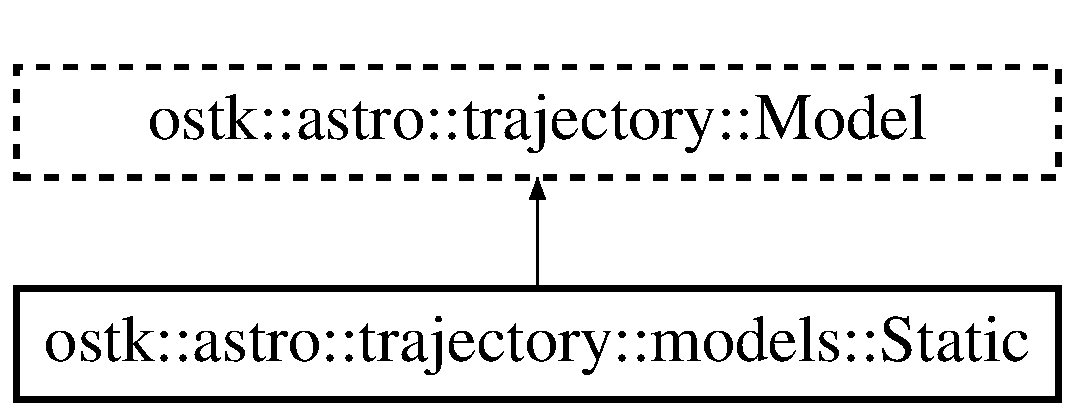
\includegraphics[height=2.000000cm]{classostk_1_1astro_1_1trajectory_1_1models_1_1_static}
\end{center}
\end{figure}
\subsection*{Public Member Functions}
\begin{DoxyCompactItemize}
\item 
\hyperlink{classostk_1_1astro_1_1trajectory_1_1models_1_1_static_a8d7240ef6b3ae12d6bdb4320b225a146}{Static} (const Position \&a\+Position)
\item 
virtual \hyperlink{classostk_1_1astro_1_1trajectory_1_1models_1_1_static}{Static} $\ast$ \hyperlink{classostk_1_1astro_1_1trajectory_1_1models_1_1_static_abe3edbc72ae2f4fbd6c2593e2aa08755}{clone} () const override
\item 
bool \hyperlink{classostk_1_1astro_1_1trajectory_1_1models_1_1_static_af74de1e58f8fc4373706264062a42faa}{operator==} (const \hyperlink{classostk_1_1astro_1_1trajectory_1_1models_1_1_static}{Static} \&a\+Static\+Model) const
\item 
bool \hyperlink{classostk_1_1astro_1_1trajectory_1_1models_1_1_static_af1f7415dfe8c549156734749ef4caaf4}{operator!=} (const \hyperlink{classostk_1_1astro_1_1trajectory_1_1models_1_1_static}{Static} \&a\+Static\+Model) const
\item 
virtual bool \hyperlink{classostk_1_1astro_1_1trajectory_1_1models_1_1_static_a5a80d75c9215af9b198c9f8653c5bc17}{is\+Defined} () const override
\item 
virtual \hyperlink{classostk_1_1astro_1_1trajectory_1_1_state}{State} \hyperlink{classostk_1_1astro_1_1trajectory_1_1models_1_1_static_a4297a74c953a105dc887a31227fbe1ff}{calculate\+State\+At} (const Instant \&an\+Instant) const override
\item 
virtual void \hyperlink{classostk_1_1astro_1_1trajectory_1_1models_1_1_static_aae663f763324f081911ea47070c9f79f}{print} (std\+::ostream \&an\+Output\+Stream, bool display\+Decorator=true) const override
\end{DoxyCompactItemize}
\subsection*{Protected Member Functions}
\begin{DoxyCompactItemize}
\item 
virtual bool \hyperlink{classostk_1_1astro_1_1trajectory_1_1models_1_1_static_a0ef36b672baa80f522135d86f3b6bb9c}{operator==} (const \hyperlink{classostk_1_1astro_1_1trajectory_1_1_model}{Model} \&a\+Model) const override
\item 
virtual bool \hyperlink{classostk_1_1astro_1_1trajectory_1_1models_1_1_static_af85efc113db69c75c1afc7db0e81297b}{operator!=} (const \hyperlink{classostk_1_1astro_1_1trajectory_1_1_model}{Model} \&a\+Model) const override
\end{DoxyCompactItemize}
\subsection*{Friends}
\begin{DoxyCompactItemize}
\item 
std\+::ostream \& \hyperlink{classostk_1_1astro_1_1trajectory_1_1models_1_1_static_a6494cb538d45101dc20cb3910455cb13}{operator$<$$<$} (std\+::ostream \&an\+Output\+Stream, const \hyperlink{classostk_1_1astro_1_1trajectory_1_1models_1_1_static}{Static} \&a\+Static\+Model)
\end{DoxyCompactItemize}


\subsection{Detailed Description}
\hyperlink{classostk_1_1astro_1_1trajectory_1_1models_1_1_static}{Static} trajectory model. 

\subsection{Constructor \& Destructor Documentation}
\mbox{\Hypertarget{classostk_1_1astro_1_1trajectory_1_1models_1_1_static_a8d7240ef6b3ae12d6bdb4320b225a146}\label{classostk_1_1astro_1_1trajectory_1_1models_1_1_static_a8d7240ef6b3ae12d6bdb4320b225a146}} 
\index{ostk\+::astro\+::trajectory\+::models\+::\+Static@{ostk\+::astro\+::trajectory\+::models\+::\+Static}!Static@{Static}}
\index{Static@{Static}!ostk\+::astro\+::trajectory\+::models\+::\+Static@{ostk\+::astro\+::trajectory\+::models\+::\+Static}}
\subsubsection{\texorpdfstring{Static()}{Static()}}
{\footnotesize\ttfamily ostk\+::astro\+::trajectory\+::models\+::\+Static\+::\+Static (\begin{DoxyParamCaption}\item[{const Position \&}]{a\+Position }\end{DoxyParamCaption})}



\subsection{Member Function Documentation}
\mbox{\Hypertarget{classostk_1_1astro_1_1trajectory_1_1models_1_1_static_a4297a74c953a105dc887a31227fbe1ff}\label{classostk_1_1astro_1_1trajectory_1_1models_1_1_static_a4297a74c953a105dc887a31227fbe1ff}} 
\index{ostk\+::astro\+::trajectory\+::models\+::\+Static@{ostk\+::astro\+::trajectory\+::models\+::\+Static}!calculate\+State\+At@{calculate\+State\+At}}
\index{calculate\+State\+At@{calculate\+State\+At}!ostk\+::astro\+::trajectory\+::models\+::\+Static@{ostk\+::astro\+::trajectory\+::models\+::\+Static}}
\subsubsection{\texorpdfstring{calculate\+State\+At()}{calculateStateAt()}}
{\footnotesize\ttfamily \hyperlink{classostk_1_1astro_1_1trajectory_1_1_state}{State} ostk\+::astro\+::trajectory\+::models\+::\+Static\+::calculate\+State\+At (\begin{DoxyParamCaption}\item[{const Instant \&}]{an\+Instant }\end{DoxyParamCaption}) const\hspace{0.3cm}{\ttfamily [override]}, {\ttfamily [virtual]}}



Implements \hyperlink{classostk_1_1astro_1_1trajectory_1_1_model_ad25eeaded2946bf73d44161b5f4e9a0e}{ostk\+::astro\+::trajectory\+::\+Model}.

\mbox{\Hypertarget{classostk_1_1astro_1_1trajectory_1_1models_1_1_static_abe3edbc72ae2f4fbd6c2593e2aa08755}\label{classostk_1_1astro_1_1trajectory_1_1models_1_1_static_abe3edbc72ae2f4fbd6c2593e2aa08755}} 
\index{ostk\+::astro\+::trajectory\+::models\+::\+Static@{ostk\+::astro\+::trajectory\+::models\+::\+Static}!clone@{clone}}
\index{clone@{clone}!ostk\+::astro\+::trajectory\+::models\+::\+Static@{ostk\+::astro\+::trajectory\+::models\+::\+Static}}
\subsubsection{\texorpdfstring{clone()}{clone()}}
{\footnotesize\ttfamily \hyperlink{classostk_1_1astro_1_1trajectory_1_1models_1_1_static}{Static} $\ast$ ostk\+::astro\+::trajectory\+::models\+::\+Static\+::clone (\begin{DoxyParamCaption}{ }\end{DoxyParamCaption}) const\hspace{0.3cm}{\ttfamily [override]}, {\ttfamily [virtual]}}



Implements \hyperlink{classostk_1_1astro_1_1trajectory_1_1_model_ad9f1467f711b07796ddc1437fb9ad9df}{ostk\+::astro\+::trajectory\+::\+Model}.

\mbox{\Hypertarget{classostk_1_1astro_1_1trajectory_1_1models_1_1_static_a5a80d75c9215af9b198c9f8653c5bc17}\label{classostk_1_1astro_1_1trajectory_1_1models_1_1_static_a5a80d75c9215af9b198c9f8653c5bc17}} 
\index{ostk\+::astro\+::trajectory\+::models\+::\+Static@{ostk\+::astro\+::trajectory\+::models\+::\+Static}!is\+Defined@{is\+Defined}}
\index{is\+Defined@{is\+Defined}!ostk\+::astro\+::trajectory\+::models\+::\+Static@{ostk\+::astro\+::trajectory\+::models\+::\+Static}}
\subsubsection{\texorpdfstring{is\+Defined()}{isDefined()}}
{\footnotesize\ttfamily bool ostk\+::astro\+::trajectory\+::models\+::\+Static\+::is\+Defined (\begin{DoxyParamCaption}{ }\end{DoxyParamCaption}) const\hspace{0.3cm}{\ttfamily [override]}, {\ttfamily [virtual]}}



Implements \hyperlink{classostk_1_1astro_1_1trajectory_1_1_model_a0d5cf6f754905f06c0ec1e39618c20a1}{ostk\+::astro\+::trajectory\+::\+Model}.

\mbox{\Hypertarget{classostk_1_1astro_1_1trajectory_1_1models_1_1_static_af1f7415dfe8c549156734749ef4caaf4}\label{classostk_1_1astro_1_1trajectory_1_1models_1_1_static_af1f7415dfe8c549156734749ef4caaf4}} 
\index{ostk\+::astro\+::trajectory\+::models\+::\+Static@{ostk\+::astro\+::trajectory\+::models\+::\+Static}!operator"!=@{operator"!=}}
\index{operator"!=@{operator"!=}!ostk\+::astro\+::trajectory\+::models\+::\+Static@{ostk\+::astro\+::trajectory\+::models\+::\+Static}}
\subsubsection{\texorpdfstring{operator"!=()}{operator!=()}\hspace{0.1cm}{\footnotesize\ttfamily [1/2]}}
{\footnotesize\ttfamily bool ostk\+::astro\+::trajectory\+::models\+::\+Static\+::operator!= (\begin{DoxyParamCaption}\item[{const \hyperlink{classostk_1_1astro_1_1trajectory_1_1models_1_1_static}{Static} \&}]{a\+Static\+Model }\end{DoxyParamCaption}) const}

\mbox{\Hypertarget{classostk_1_1astro_1_1trajectory_1_1models_1_1_static_af85efc113db69c75c1afc7db0e81297b}\label{classostk_1_1astro_1_1trajectory_1_1models_1_1_static_af85efc113db69c75c1afc7db0e81297b}} 
\index{ostk\+::astro\+::trajectory\+::models\+::\+Static@{ostk\+::astro\+::trajectory\+::models\+::\+Static}!operator"!=@{operator"!=}}
\index{operator"!=@{operator"!=}!ostk\+::astro\+::trajectory\+::models\+::\+Static@{ostk\+::astro\+::trajectory\+::models\+::\+Static}}
\subsubsection{\texorpdfstring{operator"!=()}{operator!=()}\hspace{0.1cm}{\footnotesize\ttfamily [2/2]}}
{\footnotesize\ttfamily bool ostk\+::astro\+::trajectory\+::models\+::\+Static\+::operator!= (\begin{DoxyParamCaption}\item[{const \hyperlink{classostk_1_1astro_1_1trajectory_1_1_model}{Model} \&}]{a\+Model }\end{DoxyParamCaption}) const\hspace{0.3cm}{\ttfamily [override]}, {\ttfamily [protected]}, {\ttfamily [virtual]}}



Implements \hyperlink{classostk_1_1astro_1_1trajectory_1_1_model_a2dd77b9f6939d738f3a489f26c955340}{ostk\+::astro\+::trajectory\+::\+Model}.

\mbox{\Hypertarget{classostk_1_1astro_1_1trajectory_1_1models_1_1_static_af74de1e58f8fc4373706264062a42faa}\label{classostk_1_1astro_1_1trajectory_1_1models_1_1_static_af74de1e58f8fc4373706264062a42faa}} 
\index{ostk\+::astro\+::trajectory\+::models\+::\+Static@{ostk\+::astro\+::trajectory\+::models\+::\+Static}!operator==@{operator==}}
\index{operator==@{operator==}!ostk\+::astro\+::trajectory\+::models\+::\+Static@{ostk\+::astro\+::trajectory\+::models\+::\+Static}}
\subsubsection{\texorpdfstring{operator==()}{operator==()}\hspace{0.1cm}{\footnotesize\ttfamily [1/2]}}
{\footnotesize\ttfamily bool ostk\+::astro\+::trajectory\+::models\+::\+Static\+::operator== (\begin{DoxyParamCaption}\item[{const \hyperlink{classostk_1_1astro_1_1trajectory_1_1models_1_1_static}{Static} \&}]{a\+Static\+Model }\end{DoxyParamCaption}) const}

\mbox{\Hypertarget{classostk_1_1astro_1_1trajectory_1_1models_1_1_static_a0ef36b672baa80f522135d86f3b6bb9c}\label{classostk_1_1astro_1_1trajectory_1_1models_1_1_static_a0ef36b672baa80f522135d86f3b6bb9c}} 
\index{ostk\+::astro\+::trajectory\+::models\+::\+Static@{ostk\+::astro\+::trajectory\+::models\+::\+Static}!operator==@{operator==}}
\index{operator==@{operator==}!ostk\+::astro\+::trajectory\+::models\+::\+Static@{ostk\+::astro\+::trajectory\+::models\+::\+Static}}
\subsubsection{\texorpdfstring{operator==()}{operator==()}\hspace{0.1cm}{\footnotesize\ttfamily [2/2]}}
{\footnotesize\ttfamily bool ostk\+::astro\+::trajectory\+::models\+::\+Static\+::operator== (\begin{DoxyParamCaption}\item[{const \hyperlink{classostk_1_1astro_1_1trajectory_1_1_model}{Model} \&}]{a\+Model }\end{DoxyParamCaption}) const\hspace{0.3cm}{\ttfamily [override]}, {\ttfamily [protected]}, {\ttfamily [virtual]}}



Implements \hyperlink{classostk_1_1astro_1_1trajectory_1_1_model_a874f79846e845859c070ce1b9874fc9c}{ostk\+::astro\+::trajectory\+::\+Model}.

\mbox{\Hypertarget{classostk_1_1astro_1_1trajectory_1_1models_1_1_static_aae663f763324f081911ea47070c9f79f}\label{classostk_1_1astro_1_1trajectory_1_1models_1_1_static_aae663f763324f081911ea47070c9f79f}} 
\index{ostk\+::astro\+::trajectory\+::models\+::\+Static@{ostk\+::astro\+::trajectory\+::models\+::\+Static}!print@{print}}
\index{print@{print}!ostk\+::astro\+::trajectory\+::models\+::\+Static@{ostk\+::astro\+::trajectory\+::models\+::\+Static}}
\subsubsection{\texorpdfstring{print()}{print()}}
{\footnotesize\ttfamily void ostk\+::astro\+::trajectory\+::models\+::\+Static\+::print (\begin{DoxyParamCaption}\item[{std\+::ostream \&}]{an\+Output\+Stream,  }\item[{bool}]{display\+Decorator = {\ttfamily true} }\end{DoxyParamCaption}) const\hspace{0.3cm}{\ttfamily [override]}, {\ttfamily [virtual]}}



Implements \hyperlink{classostk_1_1astro_1_1trajectory_1_1_model_a4b2098483430a820481ed50b81656e31}{ostk\+::astro\+::trajectory\+::\+Model}.



\subsection{Friends And Related Function Documentation}
\mbox{\Hypertarget{classostk_1_1astro_1_1trajectory_1_1models_1_1_static_a6494cb538d45101dc20cb3910455cb13}\label{classostk_1_1astro_1_1trajectory_1_1models_1_1_static_a6494cb538d45101dc20cb3910455cb13}} 
\index{ostk\+::astro\+::trajectory\+::models\+::\+Static@{ostk\+::astro\+::trajectory\+::models\+::\+Static}!operator$<$$<$@{operator$<$$<$}}
\index{operator$<$$<$@{operator$<$$<$}!ostk\+::astro\+::trajectory\+::models\+::\+Static@{ostk\+::astro\+::trajectory\+::models\+::\+Static}}
\subsubsection{\texorpdfstring{operator$<$$<$}{operator<<}}
{\footnotesize\ttfamily std\+::ostream\& operator$<$$<$ (\begin{DoxyParamCaption}\item[{std\+::ostream \&}]{an\+Output\+Stream,  }\item[{const \hyperlink{classostk_1_1astro_1_1trajectory_1_1models_1_1_static}{Static} \&}]{a\+Static\+Model }\end{DoxyParamCaption})\hspace{0.3cm}{\ttfamily [friend]}}



The documentation for this class was generated from the following files\+:\begin{DoxyCompactItemize}
\item 
include/\+Open\+Space\+Toolkit/\+Astrodynamics/\+Trajectory/\+Models/\hyperlink{_static_8hpp}{Static.\+hpp}\item 
src/\+Open\+Space\+Toolkit/\+Astrodynamics/\+Trajectory/\+Models/\hyperlink{_static_8cpp}{Static.\+cpp}\end{DoxyCompactItemize}

\hypertarget{classostk_1_1astro_1_1trajectory_1_1orbit_1_1models_1_1_tabulated}{}\section{ostk\+:\+:astro\+:\+:trajectory\+:\+:orbit\+:\+:models\+:\+:Tabulated Class Reference}
\label{classostk_1_1astro_1_1trajectory_1_1orbit_1_1models_1_1_tabulated}\index{ostk\+::astro\+::trajectory\+::orbit\+::models\+::\+Tabulated@{ostk\+::astro\+::trajectory\+::orbit\+::models\+::\+Tabulated}}


{\ttfamily \#include $<$Tabulated.\+hpp$>$}

Inheritance diagram for ostk\+:\+:astro\+:\+:trajectory\+:\+:orbit\+:\+:models\+:\+:Tabulated\+:\begin{figure}[H]
\begin{center}
\leavevmode
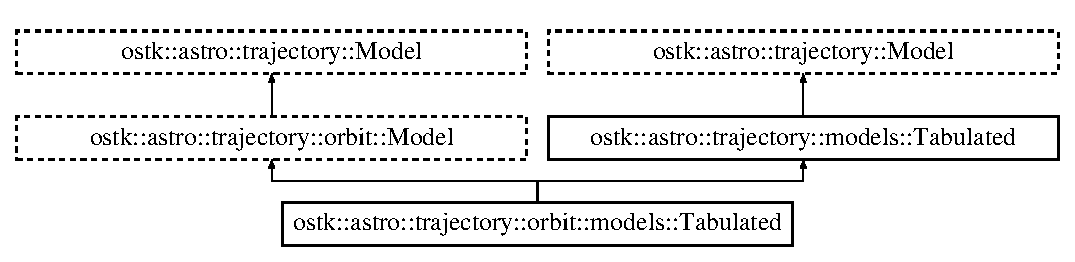
\includegraphics[height=3.000000cm]{classostk_1_1astro_1_1trajectory_1_1orbit_1_1models_1_1_tabulated}
\end{center}
\end{figure}
\subsection*{Public Member Functions}
\begin{DoxyCompactItemize}
\item 
\hyperlink{classostk_1_1astro_1_1trajectory_1_1orbit_1_1models_1_1_tabulated_aee7a0780a163332e41338e7176da97df}{Tabulated} (const Array$<$ \hyperlink{classostk_1_1astro_1_1trajectory_1_1_state}{State} $>$ \&a\+State\+Array, const Integer \&an\+Initial\+Revolution\+Number)
\item 
virtual \hyperlink{classostk_1_1astro_1_1trajectory_1_1orbit_1_1models_1_1_tabulated}{Tabulated} $\ast$ \hyperlink{classostk_1_1astro_1_1trajectory_1_1orbit_1_1models_1_1_tabulated_a53603727c33f9ff8db520831cf666142}{clone} () const override
\item 
bool \hyperlink{classostk_1_1astro_1_1trajectory_1_1orbit_1_1models_1_1_tabulated_a43b91c2c968fe65dee1a64bd3c1cdf3f}{operator==} (const \hyperlink{classostk_1_1astro_1_1trajectory_1_1orbit_1_1models_1_1_tabulated}{Tabulated} \&a\+Tabulated\+Model) const
\item 
bool \hyperlink{classostk_1_1astro_1_1trajectory_1_1orbit_1_1models_1_1_tabulated_ab50e1a3858fa4bedf4577e8d9fc30744}{operator!=} (const \hyperlink{classostk_1_1astro_1_1trajectory_1_1orbit_1_1models_1_1_tabulated}{Tabulated} \&a\+Tabulated\+Model) const
\item 
virtual bool \hyperlink{classostk_1_1astro_1_1trajectory_1_1orbit_1_1models_1_1_tabulated_ad114ba4762b54211f74f0aa3ac5eedae}{is\+Defined} () const override
\item 
virtual Instant \hyperlink{classostk_1_1astro_1_1trajectory_1_1orbit_1_1models_1_1_tabulated_a0e92ebaac60e5113989eaadc66062b75}{get\+Epoch} () const override
\item 
virtual Integer \hyperlink{classostk_1_1astro_1_1trajectory_1_1orbit_1_1models_1_1_tabulated_adbd37f167e43cedcb15358c16d62bae8}{get\+Revolution\+Number\+At\+Epoch} () const override
\item 
virtual \hyperlink{classostk_1_1astro_1_1trajectory_1_1_state}{State} \hyperlink{classostk_1_1astro_1_1trajectory_1_1orbit_1_1models_1_1_tabulated_ad7935cafe71b572b97b9df93e469d2f8}{calculate\+State\+At} (const Instant \&an\+Instant) const override
\item 
virtual Integer \hyperlink{classostk_1_1astro_1_1trajectory_1_1orbit_1_1models_1_1_tabulated_ad7aabd8943ffaa16e569e331bdfa414e}{calculate\+Revolution\+Number\+At} (const Instant \&an\+Instant) const override
\item 
virtual void \hyperlink{classostk_1_1astro_1_1trajectory_1_1orbit_1_1models_1_1_tabulated_a66be3f1f23a464c666c38a3adcc3bab5}{print} (std\+::ostream \&an\+Output\+Stream, bool display\+Decorator) const override
\end{DoxyCompactItemize}
\subsection*{Protected Member Functions}
\begin{DoxyCompactItemize}
\item 
virtual bool \hyperlink{classostk_1_1astro_1_1trajectory_1_1orbit_1_1models_1_1_tabulated_abd72010cb413d8479c097376bfebaf56}{operator==} (const \hyperlink{classostk_1_1astro_1_1trajectory_1_1_model}{trajectory\+::\+Model} \&a\+Model) const override
\item 
virtual bool \hyperlink{classostk_1_1astro_1_1trajectory_1_1orbit_1_1models_1_1_tabulated_a17610dc24fefecd03ae595cc78ef3079}{operator!=} (const \hyperlink{classostk_1_1astro_1_1trajectory_1_1_model}{trajectory\+::\+Model} \&a\+Model) const override
\end{DoxyCompactItemize}
\subsection*{Additional Inherited Members}


\subsection{Constructor \& Destructor Documentation}
\mbox{\Hypertarget{classostk_1_1astro_1_1trajectory_1_1orbit_1_1models_1_1_tabulated_aee7a0780a163332e41338e7176da97df}\label{classostk_1_1astro_1_1trajectory_1_1orbit_1_1models_1_1_tabulated_aee7a0780a163332e41338e7176da97df}} 
\index{ostk\+::astro\+::trajectory\+::orbit\+::models\+::\+Tabulated@{ostk\+::astro\+::trajectory\+::orbit\+::models\+::\+Tabulated}!Tabulated@{Tabulated}}
\index{Tabulated@{Tabulated}!ostk\+::astro\+::trajectory\+::orbit\+::models\+::\+Tabulated@{ostk\+::astro\+::trajectory\+::orbit\+::models\+::\+Tabulated}}
\subsubsection{\texorpdfstring{Tabulated()}{Tabulated()}}
{\footnotesize\ttfamily ostk\+::astro\+::trajectory\+::orbit\+::models\+::\+Tabulated\+::\+Tabulated (\begin{DoxyParamCaption}\item[{const Array$<$ \hyperlink{classostk_1_1astro_1_1trajectory_1_1_state}{State} $>$ \&}]{a\+State\+Array,  }\item[{const Integer \&}]{an\+Initial\+Revolution\+Number }\end{DoxyParamCaption})}



\subsection{Member Function Documentation}
\mbox{\Hypertarget{classostk_1_1astro_1_1trajectory_1_1orbit_1_1models_1_1_tabulated_ad7aabd8943ffaa16e569e331bdfa414e}\label{classostk_1_1astro_1_1trajectory_1_1orbit_1_1models_1_1_tabulated_ad7aabd8943ffaa16e569e331bdfa414e}} 
\index{ostk\+::astro\+::trajectory\+::orbit\+::models\+::\+Tabulated@{ostk\+::astro\+::trajectory\+::orbit\+::models\+::\+Tabulated}!calculate\+Revolution\+Number\+At@{calculate\+Revolution\+Number\+At}}
\index{calculate\+Revolution\+Number\+At@{calculate\+Revolution\+Number\+At}!ostk\+::astro\+::trajectory\+::orbit\+::models\+::\+Tabulated@{ostk\+::astro\+::trajectory\+::orbit\+::models\+::\+Tabulated}}
\subsubsection{\texorpdfstring{calculate\+Revolution\+Number\+At()}{calculateRevolutionNumberAt()}}
{\footnotesize\ttfamily Integer ostk\+::astro\+::trajectory\+::orbit\+::models\+::\+Tabulated\+::calculate\+Revolution\+Number\+At (\begin{DoxyParamCaption}\item[{const Instant \&}]{an\+Instant }\end{DoxyParamCaption}) const\hspace{0.3cm}{\ttfamily [override]}, {\ttfamily [virtual]}}



Implements \hyperlink{classostk_1_1astro_1_1trajectory_1_1orbit_1_1_model_aeecf4cc22fa9c766801936c468cc52ac}{ostk\+::astro\+::trajectory\+::orbit\+::\+Model}.

\mbox{\Hypertarget{classostk_1_1astro_1_1trajectory_1_1orbit_1_1models_1_1_tabulated_ad7935cafe71b572b97b9df93e469d2f8}\label{classostk_1_1astro_1_1trajectory_1_1orbit_1_1models_1_1_tabulated_ad7935cafe71b572b97b9df93e469d2f8}} 
\index{ostk\+::astro\+::trajectory\+::orbit\+::models\+::\+Tabulated@{ostk\+::astro\+::trajectory\+::orbit\+::models\+::\+Tabulated}!calculate\+State\+At@{calculate\+State\+At}}
\index{calculate\+State\+At@{calculate\+State\+At}!ostk\+::astro\+::trajectory\+::orbit\+::models\+::\+Tabulated@{ostk\+::astro\+::trajectory\+::orbit\+::models\+::\+Tabulated}}
\subsubsection{\texorpdfstring{calculate\+State\+At()}{calculateStateAt()}}
{\footnotesize\ttfamily \hyperlink{classostk_1_1astro_1_1trajectory_1_1_state}{State} ostk\+::astro\+::trajectory\+::orbit\+::models\+::\+Tabulated\+::calculate\+State\+At (\begin{DoxyParamCaption}\item[{const Instant \&}]{an\+Instant }\end{DoxyParamCaption}) const\hspace{0.3cm}{\ttfamily [override]}, {\ttfamily [virtual]}}



Reimplemented from \hyperlink{classostk_1_1astro_1_1trajectory_1_1models_1_1_tabulated_af2ebaa6456986636aa58c2f8666ed0b9}{ostk\+::astro\+::trajectory\+::models\+::\+Tabulated}.

\mbox{\Hypertarget{classostk_1_1astro_1_1trajectory_1_1orbit_1_1models_1_1_tabulated_a53603727c33f9ff8db520831cf666142}\label{classostk_1_1astro_1_1trajectory_1_1orbit_1_1models_1_1_tabulated_a53603727c33f9ff8db520831cf666142}} 
\index{ostk\+::astro\+::trajectory\+::orbit\+::models\+::\+Tabulated@{ostk\+::astro\+::trajectory\+::orbit\+::models\+::\+Tabulated}!clone@{clone}}
\index{clone@{clone}!ostk\+::astro\+::trajectory\+::orbit\+::models\+::\+Tabulated@{ostk\+::astro\+::trajectory\+::orbit\+::models\+::\+Tabulated}}
\subsubsection{\texorpdfstring{clone()}{clone()}}
{\footnotesize\ttfamily \hyperlink{classostk_1_1astro_1_1trajectory_1_1orbit_1_1models_1_1_tabulated}{Tabulated} $\ast$ ostk\+::astro\+::trajectory\+::orbit\+::models\+::\+Tabulated\+::clone (\begin{DoxyParamCaption}{ }\end{DoxyParamCaption}) const\hspace{0.3cm}{\ttfamily [override]}, {\ttfamily [virtual]}}



Reimplemented from \hyperlink{classostk_1_1astro_1_1trajectory_1_1models_1_1_tabulated_a553d2c4027ce269c1c2b3f4e9c65e14d}{ostk\+::astro\+::trajectory\+::models\+::\+Tabulated}.

\mbox{\Hypertarget{classostk_1_1astro_1_1trajectory_1_1orbit_1_1models_1_1_tabulated_a0e92ebaac60e5113989eaadc66062b75}\label{classostk_1_1astro_1_1trajectory_1_1orbit_1_1models_1_1_tabulated_a0e92ebaac60e5113989eaadc66062b75}} 
\index{ostk\+::astro\+::trajectory\+::orbit\+::models\+::\+Tabulated@{ostk\+::astro\+::trajectory\+::orbit\+::models\+::\+Tabulated}!get\+Epoch@{get\+Epoch}}
\index{get\+Epoch@{get\+Epoch}!ostk\+::astro\+::trajectory\+::orbit\+::models\+::\+Tabulated@{ostk\+::astro\+::trajectory\+::orbit\+::models\+::\+Tabulated}}
\subsubsection{\texorpdfstring{get\+Epoch()}{getEpoch()}}
{\footnotesize\ttfamily Instant ostk\+::astro\+::trajectory\+::orbit\+::models\+::\+Tabulated\+::get\+Epoch (\begin{DoxyParamCaption}{ }\end{DoxyParamCaption}) const\hspace{0.3cm}{\ttfamily [override]}, {\ttfamily [virtual]}}



Implements \hyperlink{classostk_1_1astro_1_1trajectory_1_1orbit_1_1_model_a22055d5ab4c22e6177a3ddb8f45f1f9b}{ostk\+::astro\+::trajectory\+::orbit\+::\+Model}.

\mbox{\Hypertarget{classostk_1_1astro_1_1trajectory_1_1orbit_1_1models_1_1_tabulated_adbd37f167e43cedcb15358c16d62bae8}\label{classostk_1_1astro_1_1trajectory_1_1orbit_1_1models_1_1_tabulated_adbd37f167e43cedcb15358c16d62bae8}} 
\index{ostk\+::astro\+::trajectory\+::orbit\+::models\+::\+Tabulated@{ostk\+::astro\+::trajectory\+::orbit\+::models\+::\+Tabulated}!get\+Revolution\+Number\+At\+Epoch@{get\+Revolution\+Number\+At\+Epoch}}
\index{get\+Revolution\+Number\+At\+Epoch@{get\+Revolution\+Number\+At\+Epoch}!ostk\+::astro\+::trajectory\+::orbit\+::models\+::\+Tabulated@{ostk\+::astro\+::trajectory\+::orbit\+::models\+::\+Tabulated}}
\subsubsection{\texorpdfstring{get\+Revolution\+Number\+At\+Epoch()}{getRevolutionNumberAtEpoch()}}
{\footnotesize\ttfamily Integer ostk\+::astro\+::trajectory\+::orbit\+::models\+::\+Tabulated\+::get\+Revolution\+Number\+At\+Epoch (\begin{DoxyParamCaption}{ }\end{DoxyParamCaption}) const\hspace{0.3cm}{\ttfamily [override]}, {\ttfamily [virtual]}}



Implements \hyperlink{classostk_1_1astro_1_1trajectory_1_1orbit_1_1_model_af3f1866f86045da2c05efe4165735cf4}{ostk\+::astro\+::trajectory\+::orbit\+::\+Model}.

\mbox{\Hypertarget{classostk_1_1astro_1_1trajectory_1_1orbit_1_1models_1_1_tabulated_ad114ba4762b54211f74f0aa3ac5eedae}\label{classostk_1_1astro_1_1trajectory_1_1orbit_1_1models_1_1_tabulated_ad114ba4762b54211f74f0aa3ac5eedae}} 
\index{ostk\+::astro\+::trajectory\+::orbit\+::models\+::\+Tabulated@{ostk\+::astro\+::trajectory\+::orbit\+::models\+::\+Tabulated}!is\+Defined@{is\+Defined}}
\index{is\+Defined@{is\+Defined}!ostk\+::astro\+::trajectory\+::orbit\+::models\+::\+Tabulated@{ostk\+::astro\+::trajectory\+::orbit\+::models\+::\+Tabulated}}
\subsubsection{\texorpdfstring{is\+Defined()}{isDefined()}}
{\footnotesize\ttfamily bool ostk\+::astro\+::trajectory\+::orbit\+::models\+::\+Tabulated\+::is\+Defined (\begin{DoxyParamCaption}{ }\end{DoxyParamCaption}) const\hspace{0.3cm}{\ttfamily [override]}, {\ttfamily [virtual]}}



Reimplemented from \hyperlink{classostk_1_1astro_1_1trajectory_1_1models_1_1_tabulated_a379da4c10a738c3f4578042c9bae0c91}{ostk\+::astro\+::trajectory\+::models\+::\+Tabulated}.

\mbox{\Hypertarget{classostk_1_1astro_1_1trajectory_1_1orbit_1_1models_1_1_tabulated_ab50e1a3858fa4bedf4577e8d9fc30744}\label{classostk_1_1astro_1_1trajectory_1_1orbit_1_1models_1_1_tabulated_ab50e1a3858fa4bedf4577e8d9fc30744}} 
\index{ostk\+::astro\+::trajectory\+::orbit\+::models\+::\+Tabulated@{ostk\+::astro\+::trajectory\+::orbit\+::models\+::\+Tabulated}!operator"!=@{operator"!=}}
\index{operator"!=@{operator"!=}!ostk\+::astro\+::trajectory\+::orbit\+::models\+::\+Tabulated@{ostk\+::astro\+::trajectory\+::orbit\+::models\+::\+Tabulated}}
\subsubsection{\texorpdfstring{operator"!=()}{operator!=()}\hspace{0.1cm}{\footnotesize\ttfamily [1/2]}}
{\footnotesize\ttfamily bool ostk\+::astro\+::trajectory\+::orbit\+::models\+::\+Tabulated\+::operator!= (\begin{DoxyParamCaption}\item[{const \hyperlink{classostk_1_1astro_1_1trajectory_1_1orbit_1_1models_1_1_tabulated}{Tabulated} \&}]{a\+Tabulated\+Model }\end{DoxyParamCaption}) const}

\mbox{\Hypertarget{classostk_1_1astro_1_1trajectory_1_1orbit_1_1models_1_1_tabulated_a17610dc24fefecd03ae595cc78ef3079}\label{classostk_1_1astro_1_1trajectory_1_1orbit_1_1models_1_1_tabulated_a17610dc24fefecd03ae595cc78ef3079}} 
\index{ostk\+::astro\+::trajectory\+::orbit\+::models\+::\+Tabulated@{ostk\+::astro\+::trajectory\+::orbit\+::models\+::\+Tabulated}!operator"!=@{operator"!=}}
\index{operator"!=@{operator"!=}!ostk\+::astro\+::trajectory\+::orbit\+::models\+::\+Tabulated@{ostk\+::astro\+::trajectory\+::orbit\+::models\+::\+Tabulated}}
\subsubsection{\texorpdfstring{operator"!=()}{operator!=()}\hspace{0.1cm}{\footnotesize\ttfamily [2/2]}}
{\footnotesize\ttfamily bool ostk\+::astro\+::trajectory\+::orbit\+::models\+::\+Tabulated\+::operator!= (\begin{DoxyParamCaption}\item[{const \hyperlink{classostk_1_1astro_1_1trajectory_1_1_model}{trajectory\+::\+Model} \&}]{a\+Model }\end{DoxyParamCaption}) const\hspace{0.3cm}{\ttfamily [override]}, {\ttfamily [protected]}, {\ttfamily [virtual]}}



Reimplemented from \hyperlink{classostk_1_1astro_1_1trajectory_1_1models_1_1_tabulated_a5e047165eb79ea50d257c2cb1bafc30d}{ostk\+::astro\+::trajectory\+::models\+::\+Tabulated}.

\mbox{\Hypertarget{classostk_1_1astro_1_1trajectory_1_1orbit_1_1models_1_1_tabulated_a43b91c2c968fe65dee1a64bd3c1cdf3f}\label{classostk_1_1astro_1_1trajectory_1_1orbit_1_1models_1_1_tabulated_a43b91c2c968fe65dee1a64bd3c1cdf3f}} 
\index{ostk\+::astro\+::trajectory\+::orbit\+::models\+::\+Tabulated@{ostk\+::astro\+::trajectory\+::orbit\+::models\+::\+Tabulated}!operator==@{operator==}}
\index{operator==@{operator==}!ostk\+::astro\+::trajectory\+::orbit\+::models\+::\+Tabulated@{ostk\+::astro\+::trajectory\+::orbit\+::models\+::\+Tabulated}}
\subsubsection{\texorpdfstring{operator==()}{operator==()}\hspace{0.1cm}{\footnotesize\ttfamily [1/2]}}
{\footnotesize\ttfamily bool ostk\+::astro\+::trajectory\+::orbit\+::models\+::\+Tabulated\+::operator== (\begin{DoxyParamCaption}\item[{const \hyperlink{classostk_1_1astro_1_1trajectory_1_1orbit_1_1models_1_1_tabulated}{Tabulated} \&}]{a\+Tabulated\+Model }\end{DoxyParamCaption}) const}

\mbox{\Hypertarget{classostk_1_1astro_1_1trajectory_1_1orbit_1_1models_1_1_tabulated_abd72010cb413d8479c097376bfebaf56}\label{classostk_1_1astro_1_1trajectory_1_1orbit_1_1models_1_1_tabulated_abd72010cb413d8479c097376bfebaf56}} 
\index{ostk\+::astro\+::trajectory\+::orbit\+::models\+::\+Tabulated@{ostk\+::astro\+::trajectory\+::orbit\+::models\+::\+Tabulated}!operator==@{operator==}}
\index{operator==@{operator==}!ostk\+::astro\+::trajectory\+::orbit\+::models\+::\+Tabulated@{ostk\+::astro\+::trajectory\+::orbit\+::models\+::\+Tabulated}}
\subsubsection{\texorpdfstring{operator==()}{operator==()}\hspace{0.1cm}{\footnotesize\ttfamily [2/2]}}
{\footnotesize\ttfamily bool ostk\+::astro\+::trajectory\+::orbit\+::models\+::\+Tabulated\+::operator== (\begin{DoxyParamCaption}\item[{const \hyperlink{classostk_1_1astro_1_1trajectory_1_1_model}{trajectory\+::\+Model} \&}]{a\+Model }\end{DoxyParamCaption}) const\hspace{0.3cm}{\ttfamily [override]}, {\ttfamily [protected]}, {\ttfamily [virtual]}}



Reimplemented from \hyperlink{classostk_1_1astro_1_1trajectory_1_1models_1_1_tabulated_a9d206aee35ebabe4b36ddfc057142f16}{ostk\+::astro\+::trajectory\+::models\+::\+Tabulated}.

\mbox{\Hypertarget{classostk_1_1astro_1_1trajectory_1_1orbit_1_1models_1_1_tabulated_a66be3f1f23a464c666c38a3adcc3bab5}\label{classostk_1_1astro_1_1trajectory_1_1orbit_1_1models_1_1_tabulated_a66be3f1f23a464c666c38a3adcc3bab5}} 
\index{ostk\+::astro\+::trajectory\+::orbit\+::models\+::\+Tabulated@{ostk\+::astro\+::trajectory\+::orbit\+::models\+::\+Tabulated}!print@{print}}
\index{print@{print}!ostk\+::astro\+::trajectory\+::orbit\+::models\+::\+Tabulated@{ostk\+::astro\+::trajectory\+::orbit\+::models\+::\+Tabulated}}
\subsubsection{\texorpdfstring{print()}{print()}}
{\footnotesize\ttfamily void ostk\+::astro\+::trajectory\+::orbit\+::models\+::\+Tabulated\+::print (\begin{DoxyParamCaption}\item[{std\+::ostream \&}]{an\+Output\+Stream,  }\item[{bool}]{display\+Decorator }\end{DoxyParamCaption}) const\hspace{0.3cm}{\ttfamily [override]}, {\ttfamily [virtual]}}



Reimplemented from \hyperlink{classostk_1_1astro_1_1trajectory_1_1models_1_1_tabulated_a330bfffa50eb77eb7f6d45cfec1e9e29}{ostk\+::astro\+::trajectory\+::models\+::\+Tabulated}.



The documentation for this class was generated from the following files\+:\begin{DoxyCompactItemize}
\item 
include/\+Open\+Space\+Toolkit/\+Astrodynamics/\+Trajectory/\+Orbit/\+Models/\hyperlink{_trajectory_2_orbit_2_models_2_tabulated_8hpp}{Tabulated.\+hpp}\item 
src/\+Open\+Space\+Toolkit/\+Astrodynamics/\+Trajectory/\+Orbit/\+Models/\hyperlink{_trajectory_2_orbit_2_models_2_tabulated_8cpp}{Tabulated.\+cpp}\end{DoxyCompactItemize}

\hypertarget{classostk_1_1astro_1_1trajectory_1_1models_1_1_tabulated}{}\section{ostk\+:\+:astro\+:\+:trajectory\+:\+:models\+:\+:Tabulated Class Reference}
\label{classostk_1_1astro_1_1trajectory_1_1models_1_1_tabulated}\index{ostk\+::astro\+::trajectory\+::models\+::\+Tabulated@{ostk\+::astro\+::trajectory\+::models\+::\+Tabulated}}


\hyperlink{classostk_1_1astro_1_1trajectory_1_1models_1_1_tabulated}{Tabulated} trajectory model.  




{\ttfamily \#include $<$Tabulated.\+hpp$>$}

Inheritance diagram for ostk\+:\+:astro\+:\+:trajectory\+:\+:models\+:\+:Tabulated\+:\begin{figure}[H]
\begin{center}
\leavevmode
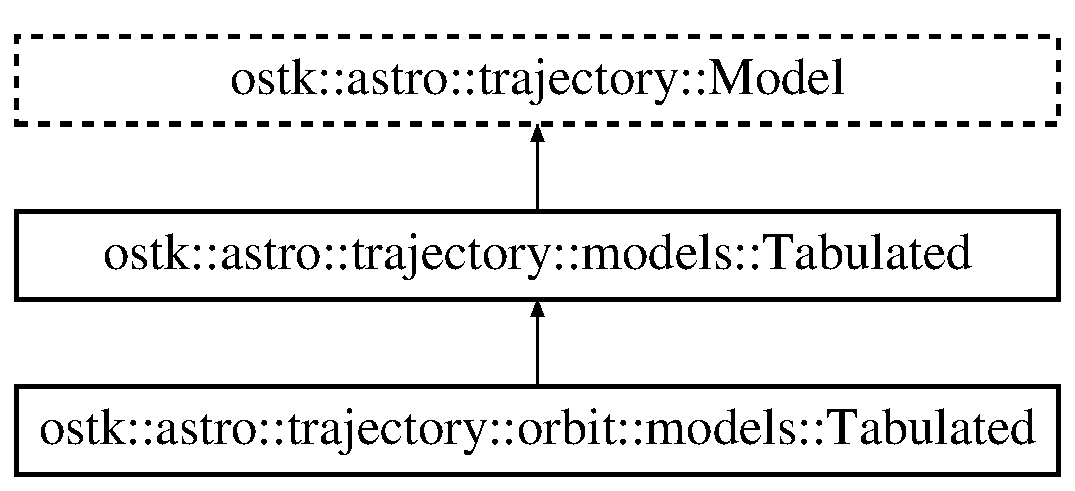
\includegraphics[height=3.000000cm]{classostk_1_1astro_1_1trajectory_1_1models_1_1_tabulated}
\end{center}
\end{figure}
\subsection*{Public Member Functions}
\begin{DoxyCompactItemize}
\item 
\hyperlink{classostk_1_1astro_1_1trajectory_1_1models_1_1_tabulated_a789aab702a52091467869fb78018b37d}{Tabulated} (const Array$<$ \hyperlink{classostk_1_1astro_1_1trajectory_1_1_state}{State} $>$ \&a\+State\+Array)
\item 
virtual \hyperlink{classostk_1_1astro_1_1trajectory_1_1models_1_1_tabulated}{Tabulated} $\ast$ \hyperlink{classostk_1_1astro_1_1trajectory_1_1models_1_1_tabulated_a553d2c4027ce269c1c2b3f4e9c65e14d}{clone} () const override
\item 
bool \hyperlink{classostk_1_1astro_1_1trajectory_1_1models_1_1_tabulated_aec2a2014af9276d9cc89cd1898a5d001}{operator==} (const \hyperlink{classostk_1_1astro_1_1trajectory_1_1models_1_1_tabulated}{Tabulated} \&a\+Tabulated\+Model) const
\item 
bool \hyperlink{classostk_1_1astro_1_1trajectory_1_1models_1_1_tabulated_a4ffc2bdbb107823f39fee423323b12cc}{operator!=} (const \hyperlink{classostk_1_1astro_1_1trajectory_1_1models_1_1_tabulated}{Tabulated} \&a\+Tabulated\+Model) const
\item 
virtual bool \hyperlink{classostk_1_1astro_1_1trajectory_1_1models_1_1_tabulated_a379da4c10a738c3f4578042c9bae0c91}{is\+Defined} () const override
\item 
Interval \hyperlink{classostk_1_1astro_1_1trajectory_1_1models_1_1_tabulated_ad385f1f0126aa00fbc33c120debff086}{get\+Interval} () const
\item 
virtual \hyperlink{classostk_1_1astro_1_1trajectory_1_1_state}{State} \hyperlink{classostk_1_1astro_1_1trajectory_1_1models_1_1_tabulated_af2ebaa6456986636aa58c2f8666ed0b9}{calculate\+State\+At} (const Instant \&an\+Instant) const override
\item 
virtual void \hyperlink{classostk_1_1astro_1_1trajectory_1_1models_1_1_tabulated_a330bfffa50eb77eb7f6d45cfec1e9e29}{print} (std\+::ostream \&an\+Output\+Stream, bool display\+Decorator=true) const override
\end{DoxyCompactItemize}
\subsection*{Static Public Member Functions}
\begin{DoxyCompactItemize}
\item 
static \hyperlink{classostk_1_1astro_1_1trajectory_1_1models_1_1_tabulated}{Tabulated} \hyperlink{classostk_1_1astro_1_1trajectory_1_1models_1_1_tabulated_a81cf8ebea4354805ab69e732bfe73d77}{Load} (const File \&a\+File)
\end{DoxyCompactItemize}
\subsection*{Protected Member Functions}
\begin{DoxyCompactItemize}
\item 
virtual bool \hyperlink{classostk_1_1astro_1_1trajectory_1_1models_1_1_tabulated_a9d206aee35ebabe4b36ddfc057142f16}{operator==} (const \hyperlink{classostk_1_1astro_1_1trajectory_1_1_model}{Model} \&a\+Model) const override
\item 
virtual bool \hyperlink{classostk_1_1astro_1_1trajectory_1_1models_1_1_tabulated_a5e047165eb79ea50d257c2cb1bafc30d}{operator!=} (const \hyperlink{classostk_1_1astro_1_1trajectory_1_1_model}{Model} \&a\+Model) const override
\end{DoxyCompactItemize}
\subsection*{Friends}
\begin{DoxyCompactItemize}
\item 
std\+::ostream \& \hyperlink{classostk_1_1astro_1_1trajectory_1_1models_1_1_tabulated_af2b779226be02822defbe40cf6d3c4b8}{operator$<$$<$} (std\+::ostream \&an\+Output\+Stream, const \hyperlink{classostk_1_1astro_1_1trajectory_1_1models_1_1_tabulated}{Tabulated} \&a\+Tabulated\+Model)
\end{DoxyCompactItemize}


\subsection{Detailed Description}
\hyperlink{classostk_1_1astro_1_1trajectory_1_1models_1_1_tabulated}{Tabulated} trajectory model. 

For now, a simple linear interpolation is performed between steps. In a future release, more advanced interpolation schemes (quadratic, spline, ...) will be provided. 

\subsection{Constructor \& Destructor Documentation}
\mbox{\Hypertarget{classostk_1_1astro_1_1trajectory_1_1models_1_1_tabulated_a789aab702a52091467869fb78018b37d}\label{classostk_1_1astro_1_1trajectory_1_1models_1_1_tabulated_a789aab702a52091467869fb78018b37d}} 
\index{ostk\+::astro\+::trajectory\+::models\+::\+Tabulated@{ostk\+::astro\+::trajectory\+::models\+::\+Tabulated}!Tabulated@{Tabulated}}
\index{Tabulated@{Tabulated}!ostk\+::astro\+::trajectory\+::models\+::\+Tabulated@{ostk\+::astro\+::trajectory\+::models\+::\+Tabulated}}
\subsubsection{\texorpdfstring{Tabulated()}{Tabulated()}}
{\footnotesize\ttfamily ostk\+::astro\+::trajectory\+::models\+::\+Tabulated\+::\+Tabulated (\begin{DoxyParamCaption}\item[{const Array$<$ \hyperlink{classostk_1_1astro_1_1trajectory_1_1_state}{State} $>$ \&}]{a\+State\+Array }\end{DoxyParamCaption})}



\subsection{Member Function Documentation}
\mbox{\Hypertarget{classostk_1_1astro_1_1trajectory_1_1models_1_1_tabulated_af2ebaa6456986636aa58c2f8666ed0b9}\label{classostk_1_1astro_1_1trajectory_1_1models_1_1_tabulated_af2ebaa6456986636aa58c2f8666ed0b9}} 
\index{ostk\+::astro\+::trajectory\+::models\+::\+Tabulated@{ostk\+::astro\+::trajectory\+::models\+::\+Tabulated}!calculate\+State\+At@{calculate\+State\+At}}
\index{calculate\+State\+At@{calculate\+State\+At}!ostk\+::astro\+::trajectory\+::models\+::\+Tabulated@{ostk\+::astro\+::trajectory\+::models\+::\+Tabulated}}
\subsubsection{\texorpdfstring{calculate\+State\+At()}{calculateStateAt()}}
{\footnotesize\ttfamily \hyperlink{classostk_1_1astro_1_1trajectory_1_1_state}{State} ostk\+::astro\+::trajectory\+::models\+::\+Tabulated\+::calculate\+State\+At (\begin{DoxyParamCaption}\item[{const Instant \&}]{an\+Instant }\end{DoxyParamCaption}) const\hspace{0.3cm}{\ttfamily [override]}, {\ttfamily [virtual]}}



Implements \hyperlink{classostk_1_1astro_1_1trajectory_1_1_model_ad25eeaded2946bf73d44161b5f4e9a0e}{ostk\+::astro\+::trajectory\+::\+Model}.



Reimplemented in \hyperlink{classostk_1_1astro_1_1trajectory_1_1orbit_1_1models_1_1_tabulated_ad7935cafe71b572b97b9df93e469d2f8}{ostk\+::astro\+::trajectory\+::orbit\+::models\+::\+Tabulated}.

\mbox{\Hypertarget{classostk_1_1astro_1_1trajectory_1_1models_1_1_tabulated_a553d2c4027ce269c1c2b3f4e9c65e14d}\label{classostk_1_1astro_1_1trajectory_1_1models_1_1_tabulated_a553d2c4027ce269c1c2b3f4e9c65e14d}} 
\index{ostk\+::astro\+::trajectory\+::models\+::\+Tabulated@{ostk\+::astro\+::trajectory\+::models\+::\+Tabulated}!clone@{clone}}
\index{clone@{clone}!ostk\+::astro\+::trajectory\+::models\+::\+Tabulated@{ostk\+::astro\+::trajectory\+::models\+::\+Tabulated}}
\subsubsection{\texorpdfstring{clone()}{clone()}}
{\footnotesize\ttfamily \hyperlink{classostk_1_1astro_1_1trajectory_1_1models_1_1_tabulated}{Tabulated} $\ast$ ostk\+::astro\+::trajectory\+::models\+::\+Tabulated\+::clone (\begin{DoxyParamCaption}{ }\end{DoxyParamCaption}) const\hspace{0.3cm}{\ttfamily [override]}, {\ttfamily [virtual]}}



Implements \hyperlink{classostk_1_1astro_1_1trajectory_1_1_model_ad9f1467f711b07796ddc1437fb9ad9df}{ostk\+::astro\+::trajectory\+::\+Model}.



Reimplemented in \hyperlink{classostk_1_1astro_1_1trajectory_1_1orbit_1_1models_1_1_tabulated_a53603727c33f9ff8db520831cf666142}{ostk\+::astro\+::trajectory\+::orbit\+::models\+::\+Tabulated}.

\mbox{\Hypertarget{classostk_1_1astro_1_1trajectory_1_1models_1_1_tabulated_ad385f1f0126aa00fbc33c120debff086}\label{classostk_1_1astro_1_1trajectory_1_1models_1_1_tabulated_ad385f1f0126aa00fbc33c120debff086}} 
\index{ostk\+::astro\+::trajectory\+::models\+::\+Tabulated@{ostk\+::astro\+::trajectory\+::models\+::\+Tabulated}!get\+Interval@{get\+Interval}}
\index{get\+Interval@{get\+Interval}!ostk\+::astro\+::trajectory\+::models\+::\+Tabulated@{ostk\+::astro\+::trajectory\+::models\+::\+Tabulated}}
\subsubsection{\texorpdfstring{get\+Interval()}{getInterval()}}
{\footnotesize\ttfamily Interval ostk\+::astro\+::trajectory\+::models\+::\+Tabulated\+::get\+Interval (\begin{DoxyParamCaption}{ }\end{DoxyParamCaption}) const}

\mbox{\Hypertarget{classostk_1_1astro_1_1trajectory_1_1models_1_1_tabulated_a379da4c10a738c3f4578042c9bae0c91}\label{classostk_1_1astro_1_1trajectory_1_1models_1_1_tabulated_a379da4c10a738c3f4578042c9bae0c91}} 
\index{ostk\+::astro\+::trajectory\+::models\+::\+Tabulated@{ostk\+::astro\+::trajectory\+::models\+::\+Tabulated}!is\+Defined@{is\+Defined}}
\index{is\+Defined@{is\+Defined}!ostk\+::astro\+::trajectory\+::models\+::\+Tabulated@{ostk\+::astro\+::trajectory\+::models\+::\+Tabulated}}
\subsubsection{\texorpdfstring{is\+Defined()}{isDefined()}}
{\footnotesize\ttfamily bool ostk\+::astro\+::trajectory\+::models\+::\+Tabulated\+::is\+Defined (\begin{DoxyParamCaption}{ }\end{DoxyParamCaption}) const\hspace{0.3cm}{\ttfamily [override]}, {\ttfamily [virtual]}}



Implements \hyperlink{classostk_1_1astro_1_1trajectory_1_1_model_a0d5cf6f754905f06c0ec1e39618c20a1}{ostk\+::astro\+::trajectory\+::\+Model}.



Reimplemented in \hyperlink{classostk_1_1astro_1_1trajectory_1_1orbit_1_1models_1_1_tabulated_ad114ba4762b54211f74f0aa3ac5eedae}{ostk\+::astro\+::trajectory\+::orbit\+::models\+::\+Tabulated}.

\mbox{\Hypertarget{classostk_1_1astro_1_1trajectory_1_1models_1_1_tabulated_a81cf8ebea4354805ab69e732bfe73d77}\label{classostk_1_1astro_1_1trajectory_1_1models_1_1_tabulated_a81cf8ebea4354805ab69e732bfe73d77}} 
\index{ostk\+::astro\+::trajectory\+::models\+::\+Tabulated@{ostk\+::astro\+::trajectory\+::models\+::\+Tabulated}!Load@{Load}}
\index{Load@{Load}!ostk\+::astro\+::trajectory\+::models\+::\+Tabulated@{ostk\+::astro\+::trajectory\+::models\+::\+Tabulated}}
\subsubsection{\texorpdfstring{Load()}{Load()}}
{\footnotesize\ttfamily static \hyperlink{classostk_1_1astro_1_1trajectory_1_1models_1_1_tabulated}{Tabulated} ostk\+::astro\+::trajectory\+::models\+::\+Tabulated\+::\+Load (\begin{DoxyParamCaption}\item[{const File \&}]{a\+File }\end{DoxyParamCaption})\hspace{0.3cm}{\ttfamily [static]}}

\mbox{\Hypertarget{classostk_1_1astro_1_1trajectory_1_1models_1_1_tabulated_a4ffc2bdbb107823f39fee423323b12cc}\label{classostk_1_1astro_1_1trajectory_1_1models_1_1_tabulated_a4ffc2bdbb107823f39fee423323b12cc}} 
\index{ostk\+::astro\+::trajectory\+::models\+::\+Tabulated@{ostk\+::astro\+::trajectory\+::models\+::\+Tabulated}!operator"!=@{operator"!=}}
\index{operator"!=@{operator"!=}!ostk\+::astro\+::trajectory\+::models\+::\+Tabulated@{ostk\+::astro\+::trajectory\+::models\+::\+Tabulated}}
\subsubsection{\texorpdfstring{operator"!=()}{operator!=()}\hspace{0.1cm}{\footnotesize\ttfamily [1/2]}}
{\footnotesize\ttfamily bool ostk\+::astro\+::trajectory\+::models\+::\+Tabulated\+::operator!= (\begin{DoxyParamCaption}\item[{const \hyperlink{classostk_1_1astro_1_1trajectory_1_1models_1_1_tabulated}{Tabulated} \&}]{a\+Tabulated\+Model }\end{DoxyParamCaption}) const}

\mbox{\Hypertarget{classostk_1_1astro_1_1trajectory_1_1models_1_1_tabulated_a5e047165eb79ea50d257c2cb1bafc30d}\label{classostk_1_1astro_1_1trajectory_1_1models_1_1_tabulated_a5e047165eb79ea50d257c2cb1bafc30d}} 
\index{ostk\+::astro\+::trajectory\+::models\+::\+Tabulated@{ostk\+::astro\+::trajectory\+::models\+::\+Tabulated}!operator"!=@{operator"!=}}
\index{operator"!=@{operator"!=}!ostk\+::astro\+::trajectory\+::models\+::\+Tabulated@{ostk\+::astro\+::trajectory\+::models\+::\+Tabulated}}
\subsubsection{\texorpdfstring{operator"!=()}{operator!=()}\hspace{0.1cm}{\footnotesize\ttfamily [2/2]}}
{\footnotesize\ttfamily bool ostk\+::astro\+::trajectory\+::models\+::\+Tabulated\+::operator!= (\begin{DoxyParamCaption}\item[{const \hyperlink{classostk_1_1astro_1_1trajectory_1_1_model}{Model} \&}]{a\+Model }\end{DoxyParamCaption}) const\hspace{0.3cm}{\ttfamily [override]}, {\ttfamily [protected]}, {\ttfamily [virtual]}}



Implements \hyperlink{classostk_1_1astro_1_1trajectory_1_1_model_a2dd77b9f6939d738f3a489f26c955340}{ostk\+::astro\+::trajectory\+::\+Model}.



Reimplemented in \hyperlink{classostk_1_1astro_1_1trajectory_1_1orbit_1_1models_1_1_tabulated_a17610dc24fefecd03ae595cc78ef3079}{ostk\+::astro\+::trajectory\+::orbit\+::models\+::\+Tabulated}.

\mbox{\Hypertarget{classostk_1_1astro_1_1trajectory_1_1models_1_1_tabulated_aec2a2014af9276d9cc89cd1898a5d001}\label{classostk_1_1astro_1_1trajectory_1_1models_1_1_tabulated_aec2a2014af9276d9cc89cd1898a5d001}} 
\index{ostk\+::astro\+::trajectory\+::models\+::\+Tabulated@{ostk\+::astro\+::trajectory\+::models\+::\+Tabulated}!operator==@{operator==}}
\index{operator==@{operator==}!ostk\+::astro\+::trajectory\+::models\+::\+Tabulated@{ostk\+::astro\+::trajectory\+::models\+::\+Tabulated}}
\subsubsection{\texorpdfstring{operator==()}{operator==()}\hspace{0.1cm}{\footnotesize\ttfamily [1/2]}}
{\footnotesize\ttfamily bool ostk\+::astro\+::trajectory\+::models\+::\+Tabulated\+::operator== (\begin{DoxyParamCaption}\item[{const \hyperlink{classostk_1_1astro_1_1trajectory_1_1models_1_1_tabulated}{Tabulated} \&}]{a\+Tabulated\+Model }\end{DoxyParamCaption}) const}

\mbox{\Hypertarget{classostk_1_1astro_1_1trajectory_1_1models_1_1_tabulated_a9d206aee35ebabe4b36ddfc057142f16}\label{classostk_1_1astro_1_1trajectory_1_1models_1_1_tabulated_a9d206aee35ebabe4b36ddfc057142f16}} 
\index{ostk\+::astro\+::trajectory\+::models\+::\+Tabulated@{ostk\+::astro\+::trajectory\+::models\+::\+Tabulated}!operator==@{operator==}}
\index{operator==@{operator==}!ostk\+::astro\+::trajectory\+::models\+::\+Tabulated@{ostk\+::astro\+::trajectory\+::models\+::\+Tabulated}}
\subsubsection{\texorpdfstring{operator==()}{operator==()}\hspace{0.1cm}{\footnotesize\ttfamily [2/2]}}
{\footnotesize\ttfamily bool ostk\+::astro\+::trajectory\+::models\+::\+Tabulated\+::operator== (\begin{DoxyParamCaption}\item[{const \hyperlink{classostk_1_1astro_1_1trajectory_1_1_model}{Model} \&}]{a\+Model }\end{DoxyParamCaption}) const\hspace{0.3cm}{\ttfamily [override]}, {\ttfamily [protected]}, {\ttfamily [virtual]}}



Implements \hyperlink{classostk_1_1astro_1_1trajectory_1_1_model_a874f79846e845859c070ce1b9874fc9c}{ostk\+::astro\+::trajectory\+::\+Model}.



Reimplemented in \hyperlink{classostk_1_1astro_1_1trajectory_1_1orbit_1_1models_1_1_tabulated_abd72010cb413d8479c097376bfebaf56}{ostk\+::astro\+::trajectory\+::orbit\+::models\+::\+Tabulated}.

\mbox{\Hypertarget{classostk_1_1astro_1_1trajectory_1_1models_1_1_tabulated_a330bfffa50eb77eb7f6d45cfec1e9e29}\label{classostk_1_1astro_1_1trajectory_1_1models_1_1_tabulated_a330bfffa50eb77eb7f6d45cfec1e9e29}} 
\index{ostk\+::astro\+::trajectory\+::models\+::\+Tabulated@{ostk\+::astro\+::trajectory\+::models\+::\+Tabulated}!print@{print}}
\index{print@{print}!ostk\+::astro\+::trajectory\+::models\+::\+Tabulated@{ostk\+::astro\+::trajectory\+::models\+::\+Tabulated}}
\subsubsection{\texorpdfstring{print()}{print()}}
{\footnotesize\ttfamily void ostk\+::astro\+::trajectory\+::models\+::\+Tabulated\+::print (\begin{DoxyParamCaption}\item[{std\+::ostream \&}]{an\+Output\+Stream,  }\item[{bool}]{display\+Decorator = {\ttfamily true} }\end{DoxyParamCaption}) const\hspace{0.3cm}{\ttfamily [override]}, {\ttfamily [virtual]}}



Implements \hyperlink{classostk_1_1astro_1_1trajectory_1_1_model_a4b2098483430a820481ed50b81656e31}{ostk\+::astro\+::trajectory\+::\+Model}.



Reimplemented in \hyperlink{classostk_1_1astro_1_1trajectory_1_1orbit_1_1models_1_1_tabulated_a66be3f1f23a464c666c38a3adcc3bab5}{ostk\+::astro\+::trajectory\+::orbit\+::models\+::\+Tabulated}.



\subsection{Friends And Related Function Documentation}
\mbox{\Hypertarget{classostk_1_1astro_1_1trajectory_1_1models_1_1_tabulated_af2b779226be02822defbe40cf6d3c4b8}\label{classostk_1_1astro_1_1trajectory_1_1models_1_1_tabulated_af2b779226be02822defbe40cf6d3c4b8}} 
\index{ostk\+::astro\+::trajectory\+::models\+::\+Tabulated@{ostk\+::astro\+::trajectory\+::models\+::\+Tabulated}!operator$<$$<$@{operator$<$$<$}}
\index{operator$<$$<$@{operator$<$$<$}!ostk\+::astro\+::trajectory\+::models\+::\+Tabulated@{ostk\+::astro\+::trajectory\+::models\+::\+Tabulated}}
\subsubsection{\texorpdfstring{operator$<$$<$}{operator<<}}
{\footnotesize\ttfamily std\+::ostream\& operator$<$$<$ (\begin{DoxyParamCaption}\item[{std\+::ostream \&}]{an\+Output\+Stream,  }\item[{const \hyperlink{classostk_1_1astro_1_1trajectory_1_1models_1_1_tabulated}{Tabulated} \&}]{a\+Tabulated\+Model }\end{DoxyParamCaption})\hspace{0.3cm}{\ttfamily [friend]}}



The documentation for this class was generated from the following files\+:\begin{DoxyCompactItemize}
\item 
include/\+Open\+Space\+Toolkit/\+Astrodynamics/\+Trajectory/\+Models/\hyperlink{_trajectory_2_models_2_tabulated_8hpp}{Tabulated.\+hpp}\item 
src/\+Open\+Space\+Toolkit/\+Astrodynamics/\+Trajectory/\+Models/\hyperlink{_trajectory_2_models_2_tabulated_8cpp}{Tabulated.\+cpp}\end{DoxyCompactItemize}

\hypertarget{classostk_1_1astro_1_1trajectory_1_1orbit_1_1models_1_1sgp4_1_1_t_l_e}{}\section{ostk\+:\+:astro\+:\+:trajectory\+:\+:orbit\+:\+:models\+:\+:sgp4\+:\+:T\+LE Class Reference}
\label{classostk_1_1astro_1_1trajectory_1_1orbit_1_1models_1_1sgp4_1_1_t_l_e}\index{ostk\+::astro\+::trajectory\+::orbit\+::models\+::sgp4\+::\+T\+LE@{ostk\+::astro\+::trajectory\+::orbit\+::models\+::sgp4\+::\+T\+LE}}


A Two-\/\+Line Element set (\hyperlink{classostk_1_1astro_1_1trajectory_1_1orbit_1_1models_1_1sgp4_1_1_t_l_e}{T\+LE}) is data format encoding a list of orbital elements of an Earth-\/orbiting object for a given point in time.  




{\ttfamily \#include $<$T\+L\+E.\+hpp$>$}

\subsection*{Public Member Functions}
\begin{DoxyCompactItemize}
\item 
\hyperlink{classostk_1_1astro_1_1trajectory_1_1orbit_1_1models_1_1sgp4_1_1_t_l_e_a57323db2c24577c2e8ddce79fa776d1e}{T\+LE} (const String \&a\+First\+Line, const String \&a\+Second\+Line)
\begin{DoxyCompactList}\small\item\em Constructor. \end{DoxyCompactList}\item 
\hyperlink{classostk_1_1astro_1_1trajectory_1_1orbit_1_1models_1_1sgp4_1_1_t_l_e_af1563fe99c5e1bf2874cf294c0e811bd}{T\+LE} (const String \&a\+Satellite\+Name, const String \&a\+First\+Line, const String \&a\+Second\+Line)
\begin{DoxyCompactList}\small\item\em Constructor. \end{DoxyCompactList}\item 
bool \hyperlink{classostk_1_1astro_1_1trajectory_1_1orbit_1_1models_1_1sgp4_1_1_t_l_e_a415bc7b3671eaa616dfd9e82f9fb9520}{operator==} (const \hyperlink{classostk_1_1astro_1_1trajectory_1_1orbit_1_1models_1_1sgp4_1_1_t_l_e}{T\+LE} \&a\+Tle) const
\begin{DoxyCompactList}\small\item\em Equal to operator. \end{DoxyCompactList}\item 
bool \hyperlink{classostk_1_1astro_1_1trajectory_1_1orbit_1_1models_1_1sgp4_1_1_t_l_e_a3b15abd9b07fb2a0851b680fe23da8f6}{operator!=} (const \hyperlink{classostk_1_1astro_1_1trajectory_1_1orbit_1_1models_1_1sgp4_1_1_t_l_e}{T\+LE} \&a\+Tle) const
\begin{DoxyCompactList}\small\item\em Not equal to operator. \end{DoxyCompactList}\item 
bool \hyperlink{classostk_1_1astro_1_1trajectory_1_1orbit_1_1models_1_1sgp4_1_1_t_l_e_aa7fa1003a2b03fb7f3829bfdd342942f}{is\+Defined} () const
\begin{DoxyCompactList}\small\item\em Check if \hyperlink{classostk_1_1astro_1_1trajectory_1_1orbit_1_1models_1_1sgp4_1_1_t_l_e}{T\+LE} is defined. \end{DoxyCompactList}\item 
String \hyperlink{classostk_1_1astro_1_1trajectory_1_1orbit_1_1models_1_1sgp4_1_1_t_l_e_a3cd38e40cec168239029eeec5bc57c23}{get\+Satellite\+Name} () const
\begin{DoxyCompactList}\small\item\em Get satellite name. \end{DoxyCompactList}\item 
String \hyperlink{classostk_1_1astro_1_1trajectory_1_1orbit_1_1models_1_1sgp4_1_1_t_l_e_ace656b8df665ed4ba7accb0adb6fd629}{get\+First\+Line} () const
\begin{DoxyCompactList}\small\item\em Get first line. \end{DoxyCompactList}\item 
String \hyperlink{classostk_1_1astro_1_1trajectory_1_1orbit_1_1models_1_1sgp4_1_1_t_l_e_a6f1f60f662a1891ce93576344989502a}{get\+Second\+Line} () const
\begin{DoxyCompactList}\small\item\em Get second line. \end{DoxyCompactList}\item 
Integer \hyperlink{classostk_1_1astro_1_1trajectory_1_1orbit_1_1models_1_1sgp4_1_1_t_l_e_a63c9241a31234dd07ee4ca4424a9df5f}{get\+Satellite\+Number} () const
\begin{DoxyCompactList}\small\item\em Get satellite number. \end{DoxyCompactList}\item 
String \hyperlink{classostk_1_1astro_1_1trajectory_1_1orbit_1_1models_1_1sgp4_1_1_t_l_e_aacb1592d95371a826ea41058f4ee6936}{get\+Classification} () const
\begin{DoxyCompactList}\small\item\em Get classification. \end{DoxyCompactList}\item 
String \hyperlink{classostk_1_1astro_1_1trajectory_1_1orbit_1_1models_1_1sgp4_1_1_t_l_e_a74fae03332b1bf5514c0850125b5c115}{get\+International\+Designator} () const
\begin{DoxyCompactList}\small\item\em Get international designator. \end{DoxyCompactList}\item 
Instant \hyperlink{classostk_1_1astro_1_1trajectory_1_1orbit_1_1models_1_1sgp4_1_1_t_l_e_a2c3580e644158b56b14868137585a73d}{get\+Epoch} () const
\begin{DoxyCompactList}\small\item\em Get epoch. \end{DoxyCompactList}\item 
Real \hyperlink{classostk_1_1astro_1_1trajectory_1_1orbit_1_1models_1_1sgp4_1_1_t_l_e_acfe76ce49653d9f735abddb908b2a2d9}{get\+Mean\+Motion\+First\+Time\+Derivative\+Divided\+By\+Two} () const
\begin{DoxyCompactList}\small\item\em Get first time derivative of the mean motion divided by two. \end{DoxyCompactList}\item 
Real \hyperlink{classostk_1_1astro_1_1trajectory_1_1orbit_1_1models_1_1sgp4_1_1_t_l_e_a7115d973dfff075411e114542bec8eeb}{get\+Mean\+Motion\+Second\+Time\+Derivative\+Divided\+By\+Six} () const
\begin{DoxyCompactList}\small\item\em Get second time derivative of mean motion divided by six. \end{DoxyCompactList}\item 
Real \hyperlink{classostk_1_1astro_1_1trajectory_1_1orbit_1_1models_1_1sgp4_1_1_t_l_e_a70763fd8cfec5751a9a5d97bdfdbf3d2}{get\+B\+Star\+Drag\+Term} () const
\begin{DoxyCompactList}\small\item\em Get B$\ast$ drag term. \end{DoxyCompactList}\item 
Integer \hyperlink{classostk_1_1astro_1_1trajectory_1_1orbit_1_1models_1_1sgp4_1_1_t_l_e_a6bbac875fb8c5d36c4ad46b7bea67b79}{get\+Ephemeris\+Type} () const
\begin{DoxyCompactList}\small\item\em Get ephemeris type (0) \end{DoxyCompactList}\item 
Integer \hyperlink{classostk_1_1astro_1_1trajectory_1_1orbit_1_1models_1_1sgp4_1_1_t_l_e_a115316d7355d615749dd7cb96d2c16c9}{get\+Element\+Set\+Number} () const
\begin{DoxyCompactList}\small\item\em Get element set number (incremented when a new \hyperlink{classostk_1_1astro_1_1trajectory_1_1orbit_1_1models_1_1sgp4_1_1_t_l_e}{T\+LE} is generated for this object) \end{DoxyCompactList}\item 
Integer \hyperlink{classostk_1_1astro_1_1trajectory_1_1orbit_1_1models_1_1sgp4_1_1_t_l_e_a9794bb184799595fefc8828c2849538c}{get\+First\+Line\+Checksum} () const
\begin{DoxyCompactList}\small\item\em Get checksum of first line. \end{DoxyCompactList}\item 
Angle \hyperlink{classostk_1_1astro_1_1trajectory_1_1orbit_1_1models_1_1sgp4_1_1_t_l_e_a5e748208f49fc10cc1b925cffa095f67}{get\+Inclination} () const
\begin{DoxyCompactList}\small\item\em Get inclination. \end{DoxyCompactList}\item 
Angle \hyperlink{classostk_1_1astro_1_1trajectory_1_1orbit_1_1models_1_1sgp4_1_1_t_l_e_af8a8a71621c85e1a0eaf4a18fc3f25e4}{get\+Raan} () const
\begin{DoxyCompactList}\small\item\em Get Right Ascension of the Ascending Node \mbox{[}R\+A\+AN\mbox{]}. \end{DoxyCompactList}\item 
Real \hyperlink{classostk_1_1astro_1_1trajectory_1_1orbit_1_1models_1_1sgp4_1_1_t_l_e_a2ea15d6fbdc6e57cfd00547d97467e48}{get\+Eccentricity} () const
\begin{DoxyCompactList}\small\item\em Get eccentricity. \end{DoxyCompactList}\item 
Angle \hyperlink{classostk_1_1astro_1_1trajectory_1_1orbit_1_1models_1_1sgp4_1_1_t_l_e_a8177e2bb63571a511e3e4ea2c853410c}{get\+Aop} () const
\begin{DoxyCompactList}\small\item\em Get Argument of Perigee \mbox{[}A\+OP\mbox{]}. \end{DoxyCompactList}\item 
Angle \hyperlink{classostk_1_1astro_1_1trajectory_1_1orbit_1_1models_1_1sgp4_1_1_t_l_e_ab5c418aedbbfb5b0bc9b401a6d850623}{get\+Mean\+Anomaly} () const
\begin{DoxyCompactList}\small\item\em Get Mean Anomaly. \end{DoxyCompactList}\item 
Derived \hyperlink{classostk_1_1astro_1_1trajectory_1_1orbit_1_1models_1_1sgp4_1_1_t_l_e_a441a9c7ee954d3d97c6d3c6cd5f7cd72}{get\+Mean\+Motion} () const
\begin{DoxyCompactList}\small\item\em Get Mean Motion. \end{DoxyCompactList}\item 
Integer \hyperlink{classostk_1_1astro_1_1trajectory_1_1orbit_1_1models_1_1sgp4_1_1_t_l_e_abc96f40aa52b9451bf791253a61365e9}{get\+Revolution\+Number\+At\+Epoch} () const
\begin{DoxyCompactList}\small\item\em Get revolution number at epoch. \end{DoxyCompactList}\end{DoxyCompactItemize}
\subsection*{Static Public Member Functions}
\begin{DoxyCompactItemize}
\item 
static \hyperlink{classostk_1_1astro_1_1trajectory_1_1orbit_1_1models_1_1sgp4_1_1_t_l_e}{T\+LE} \hyperlink{classostk_1_1astro_1_1trajectory_1_1orbit_1_1models_1_1sgp4_1_1_t_l_e_a871cdedd5bc51c9f3afa976e0597ea51}{Undefined} ()
\begin{DoxyCompactList}\small\item\em Constructs an undefined \hyperlink{classostk_1_1astro_1_1trajectory_1_1orbit_1_1models_1_1sgp4_1_1_t_l_e}{T\+LE}. \end{DoxyCompactList}\item 
static bool \hyperlink{classostk_1_1astro_1_1trajectory_1_1orbit_1_1models_1_1sgp4_1_1_t_l_e_a843f3432e8411de6b8d7e9c40d7191d2}{Can\+Parse} (const String \&a\+String)
\begin{DoxyCompactList}\small\item\em Returns true if \hyperlink{classostk_1_1astro_1_1trajectory_1_1orbit_1_1models_1_1sgp4_1_1_t_l_e}{T\+LE} can be generated from the given string. \end{DoxyCompactList}\item 
static bool \hyperlink{classostk_1_1astro_1_1trajectory_1_1orbit_1_1models_1_1sgp4_1_1_t_l_e_a1e808cef2bd2466a8d7813f2c5d5bfc4}{Can\+Parse} (const String \&a\+First\+Line, const String \&a\+Second\+Line)
\begin{DoxyCompactList}\small\item\em Returns true if \hyperlink{classostk_1_1astro_1_1trajectory_1_1orbit_1_1models_1_1sgp4_1_1_t_l_e}{T\+LE} can be generated from the given lines. \end{DoxyCompactList}\item 
static \hyperlink{classostk_1_1astro_1_1trajectory_1_1orbit_1_1models_1_1sgp4_1_1_t_l_e}{T\+LE} \hyperlink{classostk_1_1astro_1_1trajectory_1_1orbit_1_1models_1_1sgp4_1_1_t_l_e_a7f97a74af47895aa315aebc52f410d26}{Parse} (const String \&a\+String)
\begin{DoxyCompactList}\small\item\em Constructs a \hyperlink{classostk_1_1astro_1_1trajectory_1_1orbit_1_1models_1_1sgp4_1_1_t_l_e}{T\+LE} from a given string. \end{DoxyCompactList}\item 
static \hyperlink{classostk_1_1astro_1_1trajectory_1_1orbit_1_1models_1_1sgp4_1_1_t_l_e}{T\+LE} \hyperlink{classostk_1_1astro_1_1trajectory_1_1orbit_1_1models_1_1sgp4_1_1_t_l_e_a5e912145266460d05beaba326b5ace95}{Load} (const File \&a\+File)
\begin{DoxyCompactList}\small\item\em Load a \hyperlink{classostk_1_1astro_1_1trajectory_1_1orbit_1_1models_1_1sgp4_1_1_t_l_e}{T\+LE} from a given file. \end{DoxyCompactList}\end{DoxyCompactItemize}
\subsection*{Friends}
\begin{DoxyCompactItemize}
\item 
std\+::ostream \& \hyperlink{classostk_1_1astro_1_1trajectory_1_1orbit_1_1models_1_1sgp4_1_1_t_l_e_a54a7a3bca65674d5052031634f900984}{operator$<$$<$} (std\+::ostream \&an\+Output\+Stream, const \hyperlink{classostk_1_1astro_1_1trajectory_1_1orbit_1_1models_1_1sgp4_1_1_t_l_e}{T\+LE} \&a\+Tle)
\begin{DoxyCompactList}\small\item\em Output stream operator. \end{DoxyCompactList}\end{DoxyCompactItemize}


\subsection{Detailed Description}
A Two-\/\+Line Element set (\hyperlink{classostk_1_1astro_1_1trajectory_1_1orbit_1_1models_1_1sgp4_1_1_t_l_e}{T\+LE}) is data format encoding a list of orbital elements of an Earth-\/orbiting object for a given point in time. 

https\+://en.wikipedia.\+org/wiki/\+Two-\/line\+\_\+element\+\_\+set 

\subsection{Constructor \& Destructor Documentation}
\mbox{\Hypertarget{classostk_1_1astro_1_1trajectory_1_1orbit_1_1models_1_1sgp4_1_1_t_l_e_a57323db2c24577c2e8ddce79fa776d1e}\label{classostk_1_1astro_1_1trajectory_1_1orbit_1_1models_1_1sgp4_1_1_t_l_e_a57323db2c24577c2e8ddce79fa776d1e}} 
\index{ostk\+::astro\+::trajectory\+::orbit\+::models\+::sgp4\+::\+T\+LE@{ostk\+::astro\+::trajectory\+::orbit\+::models\+::sgp4\+::\+T\+LE}!T\+LE@{T\+LE}}
\index{T\+LE@{T\+LE}!ostk\+::astro\+::trajectory\+::orbit\+::models\+::sgp4\+::\+T\+LE@{ostk\+::astro\+::trajectory\+::orbit\+::models\+::sgp4\+::\+T\+LE}}
\subsubsection{\texorpdfstring{T\+L\+E()}{TLE()}\hspace{0.1cm}{\footnotesize\ttfamily [1/2]}}
{\footnotesize\ttfamily ostk\+::astro\+::trajectory\+::orbit\+::models\+::sgp4\+::\+T\+L\+E\+::\+T\+LE (\begin{DoxyParamCaption}\item[{const String \&}]{a\+First\+Line,  }\item[{const String \&}]{a\+Second\+Line }\end{DoxyParamCaption})}



Constructor. 


\begin{DoxyCode}
\hyperlink{classostk_1_1astro_1_1trajectory_1_1orbit_1_1models_1_1sgp4_1_1_t_l_e_a57323db2c24577c2e8ddce79fa776d1e}{TLE} tle(\textcolor{stringliteral}{"1 25544U 98067A   08264.51782528 -.00002182  00000-0 -11606-4 0  2927"},
        \textcolor{stringliteral}{"2 25544  51.6416 247.4627 0006703 130.5360 325.0288 15.72125391563537"}) ;
\end{DoxyCode}



\begin{DoxyParams}[1]{Parameters}
\mbox{\tt in}  & {\em a\+First\+Line} & A first line \\
\hline
\mbox{\tt in}  & {\em a\+Second\+Line} & A second line \\
\hline
\end{DoxyParams}
\mbox{\Hypertarget{classostk_1_1astro_1_1trajectory_1_1orbit_1_1models_1_1sgp4_1_1_t_l_e_af1563fe99c5e1bf2874cf294c0e811bd}\label{classostk_1_1astro_1_1trajectory_1_1orbit_1_1models_1_1sgp4_1_1_t_l_e_af1563fe99c5e1bf2874cf294c0e811bd}} 
\index{ostk\+::astro\+::trajectory\+::orbit\+::models\+::sgp4\+::\+T\+LE@{ostk\+::astro\+::trajectory\+::orbit\+::models\+::sgp4\+::\+T\+LE}!T\+LE@{T\+LE}}
\index{T\+LE@{T\+LE}!ostk\+::astro\+::trajectory\+::orbit\+::models\+::sgp4\+::\+T\+LE@{ostk\+::astro\+::trajectory\+::orbit\+::models\+::sgp4\+::\+T\+LE}}
\subsubsection{\texorpdfstring{T\+L\+E()}{TLE()}\hspace{0.1cm}{\footnotesize\ttfamily [2/2]}}
{\footnotesize\ttfamily ostk\+::astro\+::trajectory\+::orbit\+::models\+::sgp4\+::\+T\+L\+E\+::\+T\+LE (\begin{DoxyParamCaption}\item[{const String \&}]{a\+Satellite\+Name,  }\item[{const String \&}]{a\+First\+Line,  }\item[{const String \&}]{a\+Second\+Line }\end{DoxyParamCaption})}



Constructor. 


\begin{DoxyCode}
\hyperlink{classostk_1_1astro_1_1trajectory_1_1orbit_1_1models_1_1sgp4_1_1_t_l_e_a57323db2c24577c2e8ddce79fa776d1e}{TLE} tle(\textcolor{stringliteral}{"ISS (ZARYA)"},
        \textcolor{stringliteral}{"1 25544U 98067A   08264.51782528 -.00002182  00000-0 -11606-4 0  2927"},
        \textcolor{stringliteral}{"2 25544  51.6416 247.4627 0006703 130.5360 325.0288 15.72125391563537"}) ;
\end{DoxyCode}



\begin{DoxyParams}[1]{Parameters}
\mbox{\tt in}  & {\em a\+Satellite\+Name} & A satellite name \\
\hline
\mbox{\tt in}  & {\em a\+First\+Line} & A first line \\
\hline
\mbox{\tt in}  & {\em a\+Second\+Line} & A second line \\
\hline
\end{DoxyParams}


\subsection{Member Function Documentation}
\mbox{\Hypertarget{classostk_1_1astro_1_1trajectory_1_1orbit_1_1models_1_1sgp4_1_1_t_l_e_a843f3432e8411de6b8d7e9c40d7191d2}\label{classostk_1_1astro_1_1trajectory_1_1orbit_1_1models_1_1sgp4_1_1_t_l_e_a843f3432e8411de6b8d7e9c40d7191d2}} 
\index{ostk\+::astro\+::trajectory\+::orbit\+::models\+::sgp4\+::\+T\+LE@{ostk\+::astro\+::trajectory\+::orbit\+::models\+::sgp4\+::\+T\+LE}!Can\+Parse@{Can\+Parse}}
\index{Can\+Parse@{Can\+Parse}!ostk\+::astro\+::trajectory\+::orbit\+::models\+::sgp4\+::\+T\+LE@{ostk\+::astro\+::trajectory\+::orbit\+::models\+::sgp4\+::\+T\+LE}}
\subsubsection{\texorpdfstring{Can\+Parse()}{CanParse()}\hspace{0.1cm}{\footnotesize\ttfamily [1/2]}}
{\footnotesize\ttfamily bool ostk\+::astro\+::trajectory\+::orbit\+::models\+::sgp4\+::\+T\+L\+E\+::\+Can\+Parse (\begin{DoxyParamCaption}\item[{const String \&}]{a\+String }\end{DoxyParamCaption})\hspace{0.3cm}{\ttfamily [static]}}



Returns true if \hyperlink{classostk_1_1astro_1_1trajectory_1_1orbit_1_1models_1_1sgp4_1_1_t_l_e}{T\+LE} can be generated from the given string. 


\begin{DoxyCode}
\hyperlink{classostk_1_1astro_1_1trajectory_1_1orbit_1_1models_1_1sgp4_1_1_t_l_e_a843f3432e8411de6b8d7e9c40d7191d2}{TLE::CanParse}(\textcolor{stringliteral}{"1 25544U 98067A   08264.51782528 -.00002182  00000-0 -11606-4 0  2927\(\backslash\)n}
\textcolor{stringliteral}{               2 25544  51.6416 247.4627 0006703 130.5360 325.0288 15.72125391563537"}) ; \textcolor{comment}{// True}
\end{DoxyCode}



\begin{DoxyParams}[1]{Parameters}
\mbox{\tt in}  & {\em a\+String} & A string \\
\hline
\end{DoxyParams}
\begin{DoxyReturn}{Returns}
True if \hyperlink{classostk_1_1astro_1_1trajectory_1_1orbit_1_1models_1_1sgp4_1_1_t_l_e}{T\+LE} can be generated from the given string 
\end{DoxyReturn}
\mbox{\Hypertarget{classostk_1_1astro_1_1trajectory_1_1orbit_1_1models_1_1sgp4_1_1_t_l_e_a1e808cef2bd2466a8d7813f2c5d5bfc4}\label{classostk_1_1astro_1_1trajectory_1_1orbit_1_1models_1_1sgp4_1_1_t_l_e_a1e808cef2bd2466a8d7813f2c5d5bfc4}} 
\index{ostk\+::astro\+::trajectory\+::orbit\+::models\+::sgp4\+::\+T\+LE@{ostk\+::astro\+::trajectory\+::orbit\+::models\+::sgp4\+::\+T\+LE}!Can\+Parse@{Can\+Parse}}
\index{Can\+Parse@{Can\+Parse}!ostk\+::astro\+::trajectory\+::orbit\+::models\+::sgp4\+::\+T\+LE@{ostk\+::astro\+::trajectory\+::orbit\+::models\+::sgp4\+::\+T\+LE}}
\subsubsection{\texorpdfstring{Can\+Parse()}{CanParse()}\hspace{0.1cm}{\footnotesize\ttfamily [2/2]}}
{\footnotesize\ttfamily bool ostk\+::astro\+::trajectory\+::orbit\+::models\+::sgp4\+::\+T\+L\+E\+::\+Can\+Parse (\begin{DoxyParamCaption}\item[{const String \&}]{a\+First\+Line,  }\item[{const String \&}]{a\+Second\+Line }\end{DoxyParamCaption})\hspace{0.3cm}{\ttfamily [static]}}



Returns true if \hyperlink{classostk_1_1astro_1_1trajectory_1_1orbit_1_1models_1_1sgp4_1_1_t_l_e}{T\+LE} can be generated from the given lines. 


\begin{DoxyCode}
\hyperlink{classostk_1_1astro_1_1trajectory_1_1orbit_1_1models_1_1sgp4_1_1_t_l_e_a843f3432e8411de6b8d7e9c40d7191d2}{TLE::CanParse}(\textcolor{stringliteral}{"1 25544U 98067A   08264.51782528 -.00002182  00000-0 -11606-4 0  2927"},
              \textcolor{stringliteral}{"2 25544  51.6416 247.4627 0006703 130.5360 325.0288 15.72125391563537"}) ; \textcolor{comment}{// True}
\end{DoxyCode}



\begin{DoxyParams}[1]{Parameters}
\mbox{\tt in}  & {\em a\+First\+Line} & A first line \\
\hline
\mbox{\tt in}  & {\em a\+Second\+Line} & A second line \\
\hline
\end{DoxyParams}
\begin{DoxyReturn}{Returns}
True if \hyperlink{classostk_1_1astro_1_1trajectory_1_1orbit_1_1models_1_1sgp4_1_1_t_l_e}{T\+LE} can be generated from the given lines 
\end{DoxyReturn}
\mbox{\Hypertarget{classostk_1_1astro_1_1trajectory_1_1orbit_1_1models_1_1sgp4_1_1_t_l_e_a8177e2bb63571a511e3e4ea2c853410c}\label{classostk_1_1astro_1_1trajectory_1_1orbit_1_1models_1_1sgp4_1_1_t_l_e_a8177e2bb63571a511e3e4ea2c853410c}} 
\index{ostk\+::astro\+::trajectory\+::orbit\+::models\+::sgp4\+::\+T\+LE@{ostk\+::astro\+::trajectory\+::orbit\+::models\+::sgp4\+::\+T\+LE}!get\+Aop@{get\+Aop}}
\index{get\+Aop@{get\+Aop}!ostk\+::astro\+::trajectory\+::orbit\+::models\+::sgp4\+::\+T\+LE@{ostk\+::astro\+::trajectory\+::orbit\+::models\+::sgp4\+::\+T\+LE}}
\subsubsection{\texorpdfstring{get\+Aop()}{getAop()}}
{\footnotesize\ttfamily Angle ostk\+::astro\+::trajectory\+::orbit\+::models\+::sgp4\+::\+T\+L\+E\+::get\+Aop (\begin{DoxyParamCaption}{ }\end{DoxyParamCaption}) const}



Get Argument of Perigee \mbox{[}A\+OP\mbox{]}. 

\begin{DoxyReturn}{Returns}
Argument of Perigee 
\end{DoxyReturn}
\mbox{\Hypertarget{classostk_1_1astro_1_1trajectory_1_1orbit_1_1models_1_1sgp4_1_1_t_l_e_a70763fd8cfec5751a9a5d97bdfdbf3d2}\label{classostk_1_1astro_1_1trajectory_1_1orbit_1_1models_1_1sgp4_1_1_t_l_e_a70763fd8cfec5751a9a5d97bdfdbf3d2}} 
\index{ostk\+::astro\+::trajectory\+::orbit\+::models\+::sgp4\+::\+T\+LE@{ostk\+::astro\+::trajectory\+::orbit\+::models\+::sgp4\+::\+T\+LE}!get\+B\+Star\+Drag\+Term@{get\+B\+Star\+Drag\+Term}}
\index{get\+B\+Star\+Drag\+Term@{get\+B\+Star\+Drag\+Term}!ostk\+::astro\+::trajectory\+::orbit\+::models\+::sgp4\+::\+T\+LE@{ostk\+::astro\+::trajectory\+::orbit\+::models\+::sgp4\+::\+T\+LE}}
\subsubsection{\texorpdfstring{get\+B\+Star\+Drag\+Term()}{getBStarDragTerm()}}
{\footnotesize\ttfamily Real ostk\+::astro\+::trajectory\+::orbit\+::models\+::sgp4\+::\+T\+L\+E\+::get\+B\+Star\+Drag\+Term (\begin{DoxyParamCaption}{ }\end{DoxyParamCaption}) const}



Get B$\ast$ drag term. 

\begin{DoxyReturn}{Returns}
B$\ast$ drag term https\+://en.wikipedia.\+org/wiki/\+B\+S\+T\+AR 
\end{DoxyReturn}
\mbox{\Hypertarget{classostk_1_1astro_1_1trajectory_1_1orbit_1_1models_1_1sgp4_1_1_t_l_e_aacb1592d95371a826ea41058f4ee6936}\label{classostk_1_1astro_1_1trajectory_1_1orbit_1_1models_1_1sgp4_1_1_t_l_e_aacb1592d95371a826ea41058f4ee6936}} 
\index{ostk\+::astro\+::trajectory\+::orbit\+::models\+::sgp4\+::\+T\+LE@{ostk\+::astro\+::trajectory\+::orbit\+::models\+::sgp4\+::\+T\+LE}!get\+Classification@{get\+Classification}}
\index{get\+Classification@{get\+Classification}!ostk\+::astro\+::trajectory\+::orbit\+::models\+::sgp4\+::\+T\+LE@{ostk\+::astro\+::trajectory\+::orbit\+::models\+::sgp4\+::\+T\+LE}}
\subsubsection{\texorpdfstring{get\+Classification()}{getClassification()}}
{\footnotesize\ttfamily String ostk\+::astro\+::trajectory\+::orbit\+::models\+::sgp4\+::\+T\+L\+E\+::get\+Classification (\begin{DoxyParamCaption}{ }\end{DoxyParamCaption}) const}



Get classification. 

\begin{DoxyReturn}{Returns}
Classification 
\end{DoxyReturn}
\mbox{\Hypertarget{classostk_1_1astro_1_1trajectory_1_1orbit_1_1models_1_1sgp4_1_1_t_l_e_a2ea15d6fbdc6e57cfd00547d97467e48}\label{classostk_1_1astro_1_1trajectory_1_1orbit_1_1models_1_1sgp4_1_1_t_l_e_a2ea15d6fbdc6e57cfd00547d97467e48}} 
\index{ostk\+::astro\+::trajectory\+::orbit\+::models\+::sgp4\+::\+T\+LE@{ostk\+::astro\+::trajectory\+::orbit\+::models\+::sgp4\+::\+T\+LE}!get\+Eccentricity@{get\+Eccentricity}}
\index{get\+Eccentricity@{get\+Eccentricity}!ostk\+::astro\+::trajectory\+::orbit\+::models\+::sgp4\+::\+T\+LE@{ostk\+::astro\+::trajectory\+::orbit\+::models\+::sgp4\+::\+T\+LE}}
\subsubsection{\texorpdfstring{get\+Eccentricity()}{getEccentricity()}}
{\footnotesize\ttfamily Real ostk\+::astro\+::trajectory\+::orbit\+::models\+::sgp4\+::\+T\+L\+E\+::get\+Eccentricity (\begin{DoxyParamCaption}{ }\end{DoxyParamCaption}) const}



Get eccentricity. 

\begin{DoxyReturn}{Returns}
Eccentricity 
\end{DoxyReturn}
\mbox{\Hypertarget{classostk_1_1astro_1_1trajectory_1_1orbit_1_1models_1_1sgp4_1_1_t_l_e_a115316d7355d615749dd7cb96d2c16c9}\label{classostk_1_1astro_1_1trajectory_1_1orbit_1_1models_1_1sgp4_1_1_t_l_e_a115316d7355d615749dd7cb96d2c16c9}} 
\index{ostk\+::astro\+::trajectory\+::orbit\+::models\+::sgp4\+::\+T\+LE@{ostk\+::astro\+::trajectory\+::orbit\+::models\+::sgp4\+::\+T\+LE}!get\+Element\+Set\+Number@{get\+Element\+Set\+Number}}
\index{get\+Element\+Set\+Number@{get\+Element\+Set\+Number}!ostk\+::astro\+::trajectory\+::orbit\+::models\+::sgp4\+::\+T\+LE@{ostk\+::astro\+::trajectory\+::orbit\+::models\+::sgp4\+::\+T\+LE}}
\subsubsection{\texorpdfstring{get\+Element\+Set\+Number()}{getElementSetNumber()}}
{\footnotesize\ttfamily Integer ostk\+::astro\+::trajectory\+::orbit\+::models\+::sgp4\+::\+T\+L\+E\+::get\+Element\+Set\+Number (\begin{DoxyParamCaption}{ }\end{DoxyParamCaption}) const}



Get element set number (incremented when a new \hyperlink{classostk_1_1astro_1_1trajectory_1_1orbit_1_1models_1_1sgp4_1_1_t_l_e}{T\+LE} is generated for this object) 

\begin{DoxyReturn}{Returns}
Element set number 
\end{DoxyReturn}
\mbox{\Hypertarget{classostk_1_1astro_1_1trajectory_1_1orbit_1_1models_1_1sgp4_1_1_t_l_e_a6bbac875fb8c5d36c4ad46b7bea67b79}\label{classostk_1_1astro_1_1trajectory_1_1orbit_1_1models_1_1sgp4_1_1_t_l_e_a6bbac875fb8c5d36c4ad46b7bea67b79}} 
\index{ostk\+::astro\+::trajectory\+::orbit\+::models\+::sgp4\+::\+T\+LE@{ostk\+::astro\+::trajectory\+::orbit\+::models\+::sgp4\+::\+T\+LE}!get\+Ephemeris\+Type@{get\+Ephemeris\+Type}}
\index{get\+Ephemeris\+Type@{get\+Ephemeris\+Type}!ostk\+::astro\+::trajectory\+::orbit\+::models\+::sgp4\+::\+T\+LE@{ostk\+::astro\+::trajectory\+::orbit\+::models\+::sgp4\+::\+T\+LE}}
\subsubsection{\texorpdfstring{get\+Ephemeris\+Type()}{getEphemerisType()}}
{\footnotesize\ttfamily Integer ostk\+::astro\+::trajectory\+::orbit\+::models\+::sgp4\+::\+T\+L\+E\+::get\+Ephemeris\+Type (\begin{DoxyParamCaption}{ }\end{DoxyParamCaption}) const}



Get ephemeris type (0) 

\begin{DoxyReturn}{Returns}
Ephemeris type 
\end{DoxyReturn}
\mbox{\Hypertarget{classostk_1_1astro_1_1trajectory_1_1orbit_1_1models_1_1sgp4_1_1_t_l_e_a2c3580e644158b56b14868137585a73d}\label{classostk_1_1astro_1_1trajectory_1_1orbit_1_1models_1_1sgp4_1_1_t_l_e_a2c3580e644158b56b14868137585a73d}} 
\index{ostk\+::astro\+::trajectory\+::orbit\+::models\+::sgp4\+::\+T\+LE@{ostk\+::astro\+::trajectory\+::orbit\+::models\+::sgp4\+::\+T\+LE}!get\+Epoch@{get\+Epoch}}
\index{get\+Epoch@{get\+Epoch}!ostk\+::astro\+::trajectory\+::orbit\+::models\+::sgp4\+::\+T\+LE@{ostk\+::astro\+::trajectory\+::orbit\+::models\+::sgp4\+::\+T\+LE}}
\subsubsection{\texorpdfstring{get\+Epoch()}{getEpoch()}}
{\footnotesize\ttfamily Instant ostk\+::astro\+::trajectory\+::orbit\+::models\+::sgp4\+::\+T\+L\+E\+::get\+Epoch (\begin{DoxyParamCaption}{ }\end{DoxyParamCaption}) const}



Get epoch. 

\begin{DoxyReturn}{Returns}
Epoch 
\end{DoxyReturn}
\mbox{\Hypertarget{classostk_1_1astro_1_1trajectory_1_1orbit_1_1models_1_1sgp4_1_1_t_l_e_ace656b8df665ed4ba7accb0adb6fd629}\label{classostk_1_1astro_1_1trajectory_1_1orbit_1_1models_1_1sgp4_1_1_t_l_e_ace656b8df665ed4ba7accb0adb6fd629}} 
\index{ostk\+::astro\+::trajectory\+::orbit\+::models\+::sgp4\+::\+T\+LE@{ostk\+::astro\+::trajectory\+::orbit\+::models\+::sgp4\+::\+T\+LE}!get\+First\+Line@{get\+First\+Line}}
\index{get\+First\+Line@{get\+First\+Line}!ostk\+::astro\+::trajectory\+::orbit\+::models\+::sgp4\+::\+T\+LE@{ostk\+::astro\+::trajectory\+::orbit\+::models\+::sgp4\+::\+T\+LE}}
\subsubsection{\texorpdfstring{get\+First\+Line()}{getFirstLine()}}
{\footnotesize\ttfamily String ostk\+::astro\+::trajectory\+::orbit\+::models\+::sgp4\+::\+T\+L\+E\+::get\+First\+Line (\begin{DoxyParamCaption}{ }\end{DoxyParamCaption}) const}



Get first line. 


\begin{DoxyCode}
\hyperlink{classostk_1_1astro_1_1trajectory_1_1orbit_1_1models_1_1sgp4_1_1_t_l_e_a57323db2c24577c2e8ddce79fa776d1e}{TLE}(\textcolor{stringliteral}{"ISS (ZARYA)"},
    \textcolor{stringliteral}{"1 25544U 98067A   08264.51782528 -.00002182  00000-0 -11606-4 0  2927"},
    \textcolor{stringliteral}{"2 25544  51.6416 247.4627 0006703 130.5360 325.0288 15.72125391563537"}).getSatelliteName() ; \textcolor{comment}{// "1
       25544U 98067A   08264.51782528 -.00002182  00000-0 -11606-4 0  2927"}
\end{DoxyCode}


\begin{DoxyReturn}{Returns}
First line 
\end{DoxyReturn}
\mbox{\Hypertarget{classostk_1_1astro_1_1trajectory_1_1orbit_1_1models_1_1sgp4_1_1_t_l_e_a9794bb184799595fefc8828c2849538c}\label{classostk_1_1astro_1_1trajectory_1_1orbit_1_1models_1_1sgp4_1_1_t_l_e_a9794bb184799595fefc8828c2849538c}} 
\index{ostk\+::astro\+::trajectory\+::orbit\+::models\+::sgp4\+::\+T\+LE@{ostk\+::astro\+::trajectory\+::orbit\+::models\+::sgp4\+::\+T\+LE}!get\+First\+Line\+Checksum@{get\+First\+Line\+Checksum}}
\index{get\+First\+Line\+Checksum@{get\+First\+Line\+Checksum}!ostk\+::astro\+::trajectory\+::orbit\+::models\+::sgp4\+::\+T\+LE@{ostk\+::astro\+::trajectory\+::orbit\+::models\+::sgp4\+::\+T\+LE}}
\subsubsection{\texorpdfstring{get\+First\+Line\+Checksum()}{getFirstLineChecksum()}}
{\footnotesize\ttfamily Integer ostk\+::astro\+::trajectory\+::orbit\+::models\+::sgp4\+::\+T\+L\+E\+::get\+First\+Line\+Checksum (\begin{DoxyParamCaption}{ }\end{DoxyParamCaption}) const}



Get checksum of first line. 

\begin{DoxyReturn}{Returns}
Checksum of first line 
\end{DoxyReturn}
\mbox{\Hypertarget{classostk_1_1astro_1_1trajectory_1_1orbit_1_1models_1_1sgp4_1_1_t_l_e_a5e748208f49fc10cc1b925cffa095f67}\label{classostk_1_1astro_1_1trajectory_1_1orbit_1_1models_1_1sgp4_1_1_t_l_e_a5e748208f49fc10cc1b925cffa095f67}} 
\index{ostk\+::astro\+::trajectory\+::orbit\+::models\+::sgp4\+::\+T\+LE@{ostk\+::astro\+::trajectory\+::orbit\+::models\+::sgp4\+::\+T\+LE}!get\+Inclination@{get\+Inclination}}
\index{get\+Inclination@{get\+Inclination}!ostk\+::astro\+::trajectory\+::orbit\+::models\+::sgp4\+::\+T\+LE@{ostk\+::astro\+::trajectory\+::orbit\+::models\+::sgp4\+::\+T\+LE}}
\subsubsection{\texorpdfstring{get\+Inclination()}{getInclination()}}
{\footnotesize\ttfamily Angle ostk\+::astro\+::trajectory\+::orbit\+::models\+::sgp4\+::\+T\+L\+E\+::get\+Inclination (\begin{DoxyParamCaption}{ }\end{DoxyParamCaption}) const}



Get inclination. 

\begin{DoxyReturn}{Returns}
Inclination 
\end{DoxyReturn}
\mbox{\Hypertarget{classostk_1_1astro_1_1trajectory_1_1orbit_1_1models_1_1sgp4_1_1_t_l_e_a74fae03332b1bf5514c0850125b5c115}\label{classostk_1_1astro_1_1trajectory_1_1orbit_1_1models_1_1sgp4_1_1_t_l_e_a74fae03332b1bf5514c0850125b5c115}} 
\index{ostk\+::astro\+::trajectory\+::orbit\+::models\+::sgp4\+::\+T\+LE@{ostk\+::astro\+::trajectory\+::orbit\+::models\+::sgp4\+::\+T\+LE}!get\+International\+Designator@{get\+International\+Designator}}
\index{get\+International\+Designator@{get\+International\+Designator}!ostk\+::astro\+::trajectory\+::orbit\+::models\+::sgp4\+::\+T\+LE@{ostk\+::astro\+::trajectory\+::orbit\+::models\+::sgp4\+::\+T\+LE}}
\subsubsection{\texorpdfstring{get\+International\+Designator()}{getInternationalDesignator()}}
{\footnotesize\ttfamily String ostk\+::astro\+::trajectory\+::orbit\+::models\+::sgp4\+::\+T\+L\+E\+::get\+International\+Designator (\begin{DoxyParamCaption}{ }\end{DoxyParamCaption}) const}



Get international designator. 

\begin{DoxyReturn}{Returns}
International designator 
\end{DoxyReturn}
\mbox{\Hypertarget{classostk_1_1astro_1_1trajectory_1_1orbit_1_1models_1_1sgp4_1_1_t_l_e_ab5c418aedbbfb5b0bc9b401a6d850623}\label{classostk_1_1astro_1_1trajectory_1_1orbit_1_1models_1_1sgp4_1_1_t_l_e_ab5c418aedbbfb5b0bc9b401a6d850623}} 
\index{ostk\+::astro\+::trajectory\+::orbit\+::models\+::sgp4\+::\+T\+LE@{ostk\+::astro\+::trajectory\+::orbit\+::models\+::sgp4\+::\+T\+LE}!get\+Mean\+Anomaly@{get\+Mean\+Anomaly}}
\index{get\+Mean\+Anomaly@{get\+Mean\+Anomaly}!ostk\+::astro\+::trajectory\+::orbit\+::models\+::sgp4\+::\+T\+LE@{ostk\+::astro\+::trajectory\+::orbit\+::models\+::sgp4\+::\+T\+LE}}
\subsubsection{\texorpdfstring{get\+Mean\+Anomaly()}{getMeanAnomaly()}}
{\footnotesize\ttfamily Angle ostk\+::astro\+::trajectory\+::orbit\+::models\+::sgp4\+::\+T\+L\+E\+::get\+Mean\+Anomaly (\begin{DoxyParamCaption}{ }\end{DoxyParamCaption}) const}



Get Mean Anomaly. 

\begin{DoxyReturn}{Returns}
Mean Anomaly 
\end{DoxyReturn}
\mbox{\Hypertarget{classostk_1_1astro_1_1trajectory_1_1orbit_1_1models_1_1sgp4_1_1_t_l_e_a441a9c7ee954d3d97c6d3c6cd5f7cd72}\label{classostk_1_1astro_1_1trajectory_1_1orbit_1_1models_1_1sgp4_1_1_t_l_e_a441a9c7ee954d3d97c6d3c6cd5f7cd72}} 
\index{ostk\+::astro\+::trajectory\+::orbit\+::models\+::sgp4\+::\+T\+LE@{ostk\+::astro\+::trajectory\+::orbit\+::models\+::sgp4\+::\+T\+LE}!get\+Mean\+Motion@{get\+Mean\+Motion}}
\index{get\+Mean\+Motion@{get\+Mean\+Motion}!ostk\+::astro\+::trajectory\+::orbit\+::models\+::sgp4\+::\+T\+LE@{ostk\+::astro\+::trajectory\+::orbit\+::models\+::sgp4\+::\+T\+LE}}
\subsubsection{\texorpdfstring{get\+Mean\+Motion()}{getMeanMotion()}}
{\footnotesize\ttfamily Derived ostk\+::astro\+::trajectory\+::orbit\+::models\+::sgp4\+::\+T\+L\+E\+::get\+Mean\+Motion (\begin{DoxyParamCaption}{ }\end{DoxyParamCaption}) const}



Get Mean Motion. 

\begin{DoxyReturn}{Returns}
Mean Motion 
\end{DoxyReturn}
\mbox{\Hypertarget{classostk_1_1astro_1_1trajectory_1_1orbit_1_1models_1_1sgp4_1_1_t_l_e_acfe76ce49653d9f735abddb908b2a2d9}\label{classostk_1_1astro_1_1trajectory_1_1orbit_1_1models_1_1sgp4_1_1_t_l_e_acfe76ce49653d9f735abddb908b2a2d9}} 
\index{ostk\+::astro\+::trajectory\+::orbit\+::models\+::sgp4\+::\+T\+LE@{ostk\+::astro\+::trajectory\+::orbit\+::models\+::sgp4\+::\+T\+LE}!get\+Mean\+Motion\+First\+Time\+Derivative\+Divided\+By\+Two@{get\+Mean\+Motion\+First\+Time\+Derivative\+Divided\+By\+Two}}
\index{get\+Mean\+Motion\+First\+Time\+Derivative\+Divided\+By\+Two@{get\+Mean\+Motion\+First\+Time\+Derivative\+Divided\+By\+Two}!ostk\+::astro\+::trajectory\+::orbit\+::models\+::sgp4\+::\+T\+LE@{ostk\+::astro\+::trajectory\+::orbit\+::models\+::sgp4\+::\+T\+LE}}
\subsubsection{\texorpdfstring{get\+Mean\+Motion\+First\+Time\+Derivative\+Divided\+By\+Two()}{getMeanMotionFirstTimeDerivativeDividedByTwo()}}
{\footnotesize\ttfamily Real ostk\+::astro\+::trajectory\+::orbit\+::models\+::sgp4\+::\+T\+L\+E\+::get\+Mean\+Motion\+First\+Time\+Derivative\+Divided\+By\+Two (\begin{DoxyParamCaption}{ }\end{DoxyParamCaption}) const}



Get first time derivative of the mean motion divided by two. 

\begin{DoxyReturn}{Returns}
First time derivative of the mean motion divided by two 
\end{DoxyReturn}
\mbox{\Hypertarget{classostk_1_1astro_1_1trajectory_1_1orbit_1_1models_1_1sgp4_1_1_t_l_e_a7115d973dfff075411e114542bec8eeb}\label{classostk_1_1astro_1_1trajectory_1_1orbit_1_1models_1_1sgp4_1_1_t_l_e_a7115d973dfff075411e114542bec8eeb}} 
\index{ostk\+::astro\+::trajectory\+::orbit\+::models\+::sgp4\+::\+T\+LE@{ostk\+::astro\+::trajectory\+::orbit\+::models\+::sgp4\+::\+T\+LE}!get\+Mean\+Motion\+Second\+Time\+Derivative\+Divided\+By\+Six@{get\+Mean\+Motion\+Second\+Time\+Derivative\+Divided\+By\+Six}}
\index{get\+Mean\+Motion\+Second\+Time\+Derivative\+Divided\+By\+Six@{get\+Mean\+Motion\+Second\+Time\+Derivative\+Divided\+By\+Six}!ostk\+::astro\+::trajectory\+::orbit\+::models\+::sgp4\+::\+T\+LE@{ostk\+::astro\+::trajectory\+::orbit\+::models\+::sgp4\+::\+T\+LE}}
\subsubsection{\texorpdfstring{get\+Mean\+Motion\+Second\+Time\+Derivative\+Divided\+By\+Six()}{getMeanMotionSecondTimeDerivativeDividedBySix()}}
{\footnotesize\ttfamily Real ostk\+::astro\+::trajectory\+::orbit\+::models\+::sgp4\+::\+T\+L\+E\+::get\+Mean\+Motion\+Second\+Time\+Derivative\+Divided\+By\+Six (\begin{DoxyParamCaption}{ }\end{DoxyParamCaption}) const}



Get second time derivative of mean motion divided by six. 

\begin{DoxyReturn}{Returns}
Second time derivative of mean motion divided by six 
\end{DoxyReturn}
\mbox{\Hypertarget{classostk_1_1astro_1_1trajectory_1_1orbit_1_1models_1_1sgp4_1_1_t_l_e_af8a8a71621c85e1a0eaf4a18fc3f25e4}\label{classostk_1_1astro_1_1trajectory_1_1orbit_1_1models_1_1sgp4_1_1_t_l_e_af8a8a71621c85e1a0eaf4a18fc3f25e4}} 
\index{ostk\+::astro\+::trajectory\+::orbit\+::models\+::sgp4\+::\+T\+LE@{ostk\+::astro\+::trajectory\+::orbit\+::models\+::sgp4\+::\+T\+LE}!get\+Raan@{get\+Raan}}
\index{get\+Raan@{get\+Raan}!ostk\+::astro\+::trajectory\+::orbit\+::models\+::sgp4\+::\+T\+LE@{ostk\+::astro\+::trajectory\+::orbit\+::models\+::sgp4\+::\+T\+LE}}
\subsubsection{\texorpdfstring{get\+Raan()}{getRaan()}}
{\footnotesize\ttfamily Angle ostk\+::astro\+::trajectory\+::orbit\+::models\+::sgp4\+::\+T\+L\+E\+::get\+Raan (\begin{DoxyParamCaption}{ }\end{DoxyParamCaption}) const}



Get Right Ascension of the Ascending Node \mbox{[}R\+A\+AN\mbox{]}. 

\begin{DoxyReturn}{Returns}
Right Ascension of the Ascending Node 
\end{DoxyReturn}
\mbox{\Hypertarget{classostk_1_1astro_1_1trajectory_1_1orbit_1_1models_1_1sgp4_1_1_t_l_e_abc96f40aa52b9451bf791253a61365e9}\label{classostk_1_1astro_1_1trajectory_1_1orbit_1_1models_1_1sgp4_1_1_t_l_e_abc96f40aa52b9451bf791253a61365e9}} 
\index{ostk\+::astro\+::trajectory\+::orbit\+::models\+::sgp4\+::\+T\+LE@{ostk\+::astro\+::trajectory\+::orbit\+::models\+::sgp4\+::\+T\+LE}!get\+Revolution\+Number\+At\+Epoch@{get\+Revolution\+Number\+At\+Epoch}}
\index{get\+Revolution\+Number\+At\+Epoch@{get\+Revolution\+Number\+At\+Epoch}!ostk\+::astro\+::trajectory\+::orbit\+::models\+::sgp4\+::\+T\+LE@{ostk\+::astro\+::trajectory\+::orbit\+::models\+::sgp4\+::\+T\+LE}}
\subsubsection{\texorpdfstring{get\+Revolution\+Number\+At\+Epoch()}{getRevolutionNumberAtEpoch()}}
{\footnotesize\ttfamily Integer ostk\+::astro\+::trajectory\+::orbit\+::models\+::sgp4\+::\+T\+L\+E\+::get\+Revolution\+Number\+At\+Epoch (\begin{DoxyParamCaption}{ }\end{DoxyParamCaption}) const}



Get revolution number at epoch. 

\begin{DoxyReturn}{Returns}
Revolution number at epoch 
\end{DoxyReturn}
\mbox{\Hypertarget{classostk_1_1astro_1_1trajectory_1_1orbit_1_1models_1_1sgp4_1_1_t_l_e_a3cd38e40cec168239029eeec5bc57c23}\label{classostk_1_1astro_1_1trajectory_1_1orbit_1_1models_1_1sgp4_1_1_t_l_e_a3cd38e40cec168239029eeec5bc57c23}} 
\index{ostk\+::astro\+::trajectory\+::orbit\+::models\+::sgp4\+::\+T\+LE@{ostk\+::astro\+::trajectory\+::orbit\+::models\+::sgp4\+::\+T\+LE}!get\+Satellite\+Name@{get\+Satellite\+Name}}
\index{get\+Satellite\+Name@{get\+Satellite\+Name}!ostk\+::astro\+::trajectory\+::orbit\+::models\+::sgp4\+::\+T\+LE@{ostk\+::astro\+::trajectory\+::orbit\+::models\+::sgp4\+::\+T\+LE}}
\subsubsection{\texorpdfstring{get\+Satellite\+Name()}{getSatelliteName()}}
{\footnotesize\ttfamily String ostk\+::astro\+::trajectory\+::orbit\+::models\+::sgp4\+::\+T\+L\+E\+::get\+Satellite\+Name (\begin{DoxyParamCaption}{ }\end{DoxyParamCaption}) const}



Get satellite name. 


\begin{DoxyCode}
\hyperlink{classostk_1_1astro_1_1trajectory_1_1orbit_1_1models_1_1sgp4_1_1_t_l_e_a57323db2c24577c2e8ddce79fa776d1e}{TLE}(\textcolor{stringliteral}{"ISS (ZARYA)"},
    \textcolor{stringliteral}{"1 25544U 98067A   08264.51782528 -.00002182  00000-0 -11606-4 0  2927"},
    \textcolor{stringliteral}{"2 25544  51.6416 247.4627 0006703 130.5360 325.0288 15.72125391563537"}).getSatelliteName() ; \textcolor{comment}{// "ISS
       (ZARYA)"}
\end{DoxyCode}


\begin{DoxyReturn}{Returns}
Satellite name 
\end{DoxyReturn}
\mbox{\Hypertarget{classostk_1_1astro_1_1trajectory_1_1orbit_1_1models_1_1sgp4_1_1_t_l_e_a63c9241a31234dd07ee4ca4424a9df5f}\label{classostk_1_1astro_1_1trajectory_1_1orbit_1_1models_1_1sgp4_1_1_t_l_e_a63c9241a31234dd07ee4ca4424a9df5f}} 
\index{ostk\+::astro\+::trajectory\+::orbit\+::models\+::sgp4\+::\+T\+LE@{ostk\+::astro\+::trajectory\+::orbit\+::models\+::sgp4\+::\+T\+LE}!get\+Satellite\+Number@{get\+Satellite\+Number}}
\index{get\+Satellite\+Number@{get\+Satellite\+Number}!ostk\+::astro\+::trajectory\+::orbit\+::models\+::sgp4\+::\+T\+LE@{ostk\+::astro\+::trajectory\+::orbit\+::models\+::sgp4\+::\+T\+LE}}
\subsubsection{\texorpdfstring{get\+Satellite\+Number()}{getSatelliteNumber()}}
{\footnotesize\ttfamily Integer ostk\+::astro\+::trajectory\+::orbit\+::models\+::sgp4\+::\+T\+L\+E\+::get\+Satellite\+Number (\begin{DoxyParamCaption}{ }\end{DoxyParamCaption}) const}



Get satellite number. 

\begin{DoxyReturn}{Returns}
Satellite number 
\end{DoxyReturn}
\mbox{\Hypertarget{classostk_1_1astro_1_1trajectory_1_1orbit_1_1models_1_1sgp4_1_1_t_l_e_a6f1f60f662a1891ce93576344989502a}\label{classostk_1_1astro_1_1trajectory_1_1orbit_1_1models_1_1sgp4_1_1_t_l_e_a6f1f60f662a1891ce93576344989502a}} 
\index{ostk\+::astro\+::trajectory\+::orbit\+::models\+::sgp4\+::\+T\+LE@{ostk\+::astro\+::trajectory\+::orbit\+::models\+::sgp4\+::\+T\+LE}!get\+Second\+Line@{get\+Second\+Line}}
\index{get\+Second\+Line@{get\+Second\+Line}!ostk\+::astro\+::trajectory\+::orbit\+::models\+::sgp4\+::\+T\+LE@{ostk\+::astro\+::trajectory\+::orbit\+::models\+::sgp4\+::\+T\+LE}}
\subsubsection{\texorpdfstring{get\+Second\+Line()}{getSecondLine()}}
{\footnotesize\ttfamily String ostk\+::astro\+::trajectory\+::orbit\+::models\+::sgp4\+::\+T\+L\+E\+::get\+Second\+Line (\begin{DoxyParamCaption}{ }\end{DoxyParamCaption}) const}



Get second line. 


\begin{DoxyCode}
\hyperlink{classostk_1_1astro_1_1trajectory_1_1orbit_1_1models_1_1sgp4_1_1_t_l_e_a57323db2c24577c2e8ddce79fa776d1e}{TLE}(\textcolor{stringliteral}{"ISS (ZARYA)"},
    \textcolor{stringliteral}{"1 25544U 98067A   08264.51782528 -.00002182  00000-0 -11606-4 0  2927"},
    \textcolor{stringliteral}{"2 25544  51.6416 247.4627 0006703 130.5360 325.0288 15.72125391563537"}).getSatelliteName() ; \textcolor{comment}{// "2
       25544  51.6416 247.4627 0006703 130.5360 325.0288 15.72125391563537"}
\end{DoxyCode}


\begin{DoxyReturn}{Returns}
Second line 
\end{DoxyReturn}
\mbox{\Hypertarget{classostk_1_1astro_1_1trajectory_1_1orbit_1_1models_1_1sgp4_1_1_t_l_e_aa7fa1003a2b03fb7f3829bfdd342942f}\label{classostk_1_1astro_1_1trajectory_1_1orbit_1_1models_1_1sgp4_1_1_t_l_e_aa7fa1003a2b03fb7f3829bfdd342942f}} 
\index{ostk\+::astro\+::trajectory\+::orbit\+::models\+::sgp4\+::\+T\+LE@{ostk\+::astro\+::trajectory\+::orbit\+::models\+::sgp4\+::\+T\+LE}!is\+Defined@{is\+Defined}}
\index{is\+Defined@{is\+Defined}!ostk\+::astro\+::trajectory\+::orbit\+::models\+::sgp4\+::\+T\+LE@{ostk\+::astro\+::trajectory\+::orbit\+::models\+::sgp4\+::\+T\+LE}}
\subsubsection{\texorpdfstring{is\+Defined()}{isDefined()}}
{\footnotesize\ttfamily bool ostk\+::astro\+::trajectory\+::orbit\+::models\+::sgp4\+::\+T\+L\+E\+::is\+Defined (\begin{DoxyParamCaption}{ }\end{DoxyParamCaption}) const}



Check if \hyperlink{classostk_1_1astro_1_1trajectory_1_1orbit_1_1models_1_1sgp4_1_1_t_l_e}{T\+LE} is defined. 


\begin{DoxyCode}
\hyperlink{classostk_1_1astro_1_1trajectory_1_1orbit_1_1models_1_1sgp4_1_1_t_l_e_a57323db2c24577c2e8ddce79fa776d1e}{TLE}(\textcolor{stringliteral}{"1 25544U 98067A   08264.51782528 -.00002182  00000-0 -11606-4 0  2927"},
    \textcolor{stringliteral}{"2 25544  51.6416 247.4627 0006703 130.5360 325.0288 15.72125391563537"}).isDefined() ; \textcolor{comment}{// True}
\end{DoxyCode}


\begin{DoxyReturn}{Returns}
True if \hyperlink{classostk_1_1astro_1_1trajectory_1_1orbit_1_1models_1_1sgp4_1_1_t_l_e}{T\+LE} is defined 
\end{DoxyReturn}
\mbox{\Hypertarget{classostk_1_1astro_1_1trajectory_1_1orbit_1_1models_1_1sgp4_1_1_t_l_e_a5e912145266460d05beaba326b5ace95}\label{classostk_1_1astro_1_1trajectory_1_1orbit_1_1models_1_1sgp4_1_1_t_l_e_a5e912145266460d05beaba326b5ace95}} 
\index{ostk\+::astro\+::trajectory\+::orbit\+::models\+::sgp4\+::\+T\+LE@{ostk\+::astro\+::trajectory\+::orbit\+::models\+::sgp4\+::\+T\+LE}!Load@{Load}}
\index{Load@{Load}!ostk\+::astro\+::trajectory\+::orbit\+::models\+::sgp4\+::\+T\+LE@{ostk\+::astro\+::trajectory\+::orbit\+::models\+::sgp4\+::\+T\+LE}}
\subsubsection{\texorpdfstring{Load()}{Load()}}
{\footnotesize\ttfamily \hyperlink{classostk_1_1astro_1_1trajectory_1_1orbit_1_1models_1_1sgp4_1_1_t_l_e}{T\+LE} ostk\+::astro\+::trajectory\+::orbit\+::models\+::sgp4\+::\+T\+L\+E\+::\+Load (\begin{DoxyParamCaption}\item[{const File \&}]{a\+File }\end{DoxyParamCaption})\hspace{0.3cm}{\ttfamily [static]}}



Load a \hyperlink{classostk_1_1astro_1_1trajectory_1_1orbit_1_1models_1_1sgp4_1_1_t_l_e}{T\+LE} from a given file. 


\begin{DoxyCode}
\hyperlink{classostk_1_1astro_1_1trajectory_1_1orbit_1_1models_1_1sgp4_1_1_t_l_e_a57323db2c24577c2e8ddce79fa776d1e}{TLE} tle = TLE::File(File::Path(Path::String(\textcolor{stringliteral}{"/path/to/file.tle"}))) ;
\end{DoxyCode}



\begin{DoxyParams}[1]{Parameters}
\mbox{\tt in}  & {\em a\+File} & A file \\
\hline
\end{DoxyParams}
\begin{DoxyReturn}{Returns}
\hyperlink{classostk_1_1astro_1_1trajectory_1_1orbit_1_1models_1_1sgp4_1_1_t_l_e}{T\+LE} 
\end{DoxyReturn}
\mbox{\Hypertarget{classostk_1_1astro_1_1trajectory_1_1orbit_1_1models_1_1sgp4_1_1_t_l_e_a3b15abd9b07fb2a0851b680fe23da8f6}\label{classostk_1_1astro_1_1trajectory_1_1orbit_1_1models_1_1sgp4_1_1_t_l_e_a3b15abd9b07fb2a0851b680fe23da8f6}} 
\index{ostk\+::astro\+::trajectory\+::orbit\+::models\+::sgp4\+::\+T\+LE@{ostk\+::astro\+::trajectory\+::orbit\+::models\+::sgp4\+::\+T\+LE}!operator"!=@{operator"!=}}
\index{operator"!=@{operator"!=}!ostk\+::astro\+::trajectory\+::orbit\+::models\+::sgp4\+::\+T\+LE@{ostk\+::astro\+::trajectory\+::orbit\+::models\+::sgp4\+::\+T\+LE}}
\subsubsection{\texorpdfstring{operator"!=()}{operator!=()}}
{\footnotesize\ttfamily bool ostk\+::astro\+::trajectory\+::orbit\+::models\+::sgp4\+::\+T\+L\+E\+::operator!= (\begin{DoxyParamCaption}\item[{const \hyperlink{classostk_1_1astro_1_1trajectory_1_1orbit_1_1models_1_1sgp4_1_1_t_l_e}{T\+LE} \&}]{a\+Tle }\end{DoxyParamCaption}) const}



Not equal to operator. 


\begin{DoxyCode}
\hyperlink{classostk_1_1astro_1_1trajectory_1_1orbit_1_1models_1_1sgp4_1_1_t_l_e_a57323db2c24577c2e8ddce79fa776d1e}{TLE}(\textcolor{stringliteral}{"..."}, \textcolor{stringliteral}{"..."}) != \hyperlink{classostk_1_1astro_1_1trajectory_1_1orbit_1_1models_1_1sgp4_1_1_t_l_e_a57323db2c24577c2e8ddce79fa776d1e}{TLE}(\textcolor{stringliteral}{"..."}, \textcolor{stringliteral}{"..."}) ;
\end{DoxyCode}



\begin{DoxyParams}[1]{Parameters}
\mbox{\tt in}  & {\em a\+Tle} & A \hyperlink{classostk_1_1astro_1_1trajectory_1_1orbit_1_1models_1_1sgp4_1_1_t_l_e}{T\+LE} \\
\hline
\end{DoxyParams}
\begin{DoxyReturn}{Returns}
True if T\+L\+Es are not equal 
\end{DoxyReturn}
\mbox{\Hypertarget{classostk_1_1astro_1_1trajectory_1_1orbit_1_1models_1_1sgp4_1_1_t_l_e_a415bc7b3671eaa616dfd9e82f9fb9520}\label{classostk_1_1astro_1_1trajectory_1_1orbit_1_1models_1_1sgp4_1_1_t_l_e_a415bc7b3671eaa616dfd9e82f9fb9520}} 
\index{ostk\+::astro\+::trajectory\+::orbit\+::models\+::sgp4\+::\+T\+LE@{ostk\+::astro\+::trajectory\+::orbit\+::models\+::sgp4\+::\+T\+LE}!operator==@{operator==}}
\index{operator==@{operator==}!ostk\+::astro\+::trajectory\+::orbit\+::models\+::sgp4\+::\+T\+LE@{ostk\+::astro\+::trajectory\+::orbit\+::models\+::sgp4\+::\+T\+LE}}
\subsubsection{\texorpdfstring{operator==()}{operator==()}}
{\footnotesize\ttfamily bool ostk\+::astro\+::trajectory\+::orbit\+::models\+::sgp4\+::\+T\+L\+E\+::operator== (\begin{DoxyParamCaption}\item[{const \hyperlink{classostk_1_1astro_1_1trajectory_1_1orbit_1_1models_1_1sgp4_1_1_t_l_e}{T\+LE} \&}]{a\+Tle }\end{DoxyParamCaption}) const}



Equal to operator. 


\begin{DoxyCode}
\hyperlink{classostk_1_1astro_1_1trajectory_1_1orbit_1_1models_1_1sgp4_1_1_t_l_e_a57323db2c24577c2e8ddce79fa776d1e}{TLE}(\textcolor{stringliteral}{"..."}, \textcolor{stringliteral}{"..."}) == \hyperlink{classostk_1_1astro_1_1trajectory_1_1orbit_1_1models_1_1sgp4_1_1_t_l_e_a57323db2c24577c2e8ddce79fa776d1e}{TLE}(\textcolor{stringliteral}{"..."}, \textcolor{stringliteral}{"..."}) ;
\end{DoxyCode}



\begin{DoxyParams}[1]{Parameters}
\mbox{\tt in}  & {\em a\+Tle} & A \hyperlink{classostk_1_1astro_1_1trajectory_1_1orbit_1_1models_1_1sgp4_1_1_t_l_e}{T\+LE} \\
\hline
\end{DoxyParams}
\begin{DoxyReturn}{Returns}
True if T\+L\+Es are equal 
\end{DoxyReturn}
\mbox{\Hypertarget{classostk_1_1astro_1_1trajectory_1_1orbit_1_1models_1_1sgp4_1_1_t_l_e_a7f97a74af47895aa315aebc52f410d26}\label{classostk_1_1astro_1_1trajectory_1_1orbit_1_1models_1_1sgp4_1_1_t_l_e_a7f97a74af47895aa315aebc52f410d26}} 
\index{ostk\+::astro\+::trajectory\+::orbit\+::models\+::sgp4\+::\+T\+LE@{ostk\+::astro\+::trajectory\+::orbit\+::models\+::sgp4\+::\+T\+LE}!Parse@{Parse}}
\index{Parse@{Parse}!ostk\+::astro\+::trajectory\+::orbit\+::models\+::sgp4\+::\+T\+LE@{ostk\+::astro\+::trajectory\+::orbit\+::models\+::sgp4\+::\+T\+LE}}
\subsubsection{\texorpdfstring{Parse()}{Parse()}}
{\footnotesize\ttfamily \hyperlink{classostk_1_1astro_1_1trajectory_1_1orbit_1_1models_1_1sgp4_1_1_t_l_e}{T\+LE} ostk\+::astro\+::trajectory\+::orbit\+::models\+::sgp4\+::\+T\+L\+E\+::\+Parse (\begin{DoxyParamCaption}\item[{const String \&}]{a\+String }\end{DoxyParamCaption})\hspace{0.3cm}{\ttfamily [static]}}



Constructs a \hyperlink{classostk_1_1astro_1_1trajectory_1_1orbit_1_1models_1_1sgp4_1_1_t_l_e}{T\+LE} from a given string. 


\begin{DoxyCode}
\hyperlink{classostk_1_1astro_1_1trajectory_1_1orbit_1_1models_1_1sgp4_1_1_t_l_e_a57323db2c24577c2e8ddce79fa776d1e}{TLE} tle = \hyperlink{classostk_1_1astro_1_1trajectory_1_1orbit_1_1models_1_1sgp4_1_1_t_l_e_a7f97a74af47895aa315aebc52f410d26}{TLE::Parse}(\textcolor{stringliteral}{"1 25544U 98067A   08264.51782528 -.00002182  00000-0 -11606-4 0  2927\(\backslash\)n}
\textcolor{stringliteral}{                      2 25544  51.6416 247.4627 0006703 130.5360 325.0288 15.72125391563537"}) ;
\end{DoxyCode}



\begin{DoxyParams}[1]{Parameters}
\mbox{\tt in}  & {\em a\+String} & A string \\
\hline
\end{DoxyParams}
\begin{DoxyReturn}{Returns}
\hyperlink{classostk_1_1astro_1_1trajectory_1_1orbit_1_1models_1_1sgp4_1_1_t_l_e}{T\+LE} 
\end{DoxyReturn}
\mbox{\Hypertarget{classostk_1_1astro_1_1trajectory_1_1orbit_1_1models_1_1sgp4_1_1_t_l_e_a871cdedd5bc51c9f3afa976e0597ea51}\label{classostk_1_1astro_1_1trajectory_1_1orbit_1_1models_1_1sgp4_1_1_t_l_e_a871cdedd5bc51c9f3afa976e0597ea51}} 
\index{ostk\+::astro\+::trajectory\+::orbit\+::models\+::sgp4\+::\+T\+LE@{ostk\+::astro\+::trajectory\+::orbit\+::models\+::sgp4\+::\+T\+LE}!Undefined@{Undefined}}
\index{Undefined@{Undefined}!ostk\+::astro\+::trajectory\+::orbit\+::models\+::sgp4\+::\+T\+LE@{ostk\+::astro\+::trajectory\+::orbit\+::models\+::sgp4\+::\+T\+LE}}
\subsubsection{\texorpdfstring{Undefined()}{Undefined()}}
{\footnotesize\ttfamily \hyperlink{classostk_1_1astro_1_1trajectory_1_1orbit_1_1models_1_1sgp4_1_1_t_l_e}{T\+LE} ostk\+::astro\+::trajectory\+::orbit\+::models\+::sgp4\+::\+T\+L\+E\+::\+Undefined (\begin{DoxyParamCaption}{ }\end{DoxyParamCaption})\hspace{0.3cm}{\ttfamily [static]}}



Constructs an undefined \hyperlink{classostk_1_1astro_1_1trajectory_1_1orbit_1_1models_1_1sgp4_1_1_t_l_e}{T\+LE}. 


\begin{DoxyCode}
\hyperlink{classostk_1_1astro_1_1trajectory_1_1orbit_1_1models_1_1sgp4_1_1_t_l_e_a57323db2c24577c2e8ddce79fa776d1e}{TLE} tle = \hyperlink{classostk_1_1astro_1_1trajectory_1_1orbit_1_1models_1_1sgp4_1_1_t_l_e_a871cdedd5bc51c9f3afa976e0597ea51}{TLE::Undefined}() ; \textcolor{comment}{// Undefined}
\end{DoxyCode}


\begin{DoxyReturn}{Returns}
Undefined \hyperlink{classostk_1_1astro_1_1trajectory_1_1orbit_1_1models_1_1sgp4_1_1_t_l_e}{T\+LE} 
\end{DoxyReturn}


\subsection{Friends And Related Function Documentation}
\mbox{\Hypertarget{classostk_1_1astro_1_1trajectory_1_1orbit_1_1models_1_1sgp4_1_1_t_l_e_a54a7a3bca65674d5052031634f900984}\label{classostk_1_1astro_1_1trajectory_1_1orbit_1_1models_1_1sgp4_1_1_t_l_e_a54a7a3bca65674d5052031634f900984}} 
\index{ostk\+::astro\+::trajectory\+::orbit\+::models\+::sgp4\+::\+T\+LE@{ostk\+::astro\+::trajectory\+::orbit\+::models\+::sgp4\+::\+T\+LE}!operator$<$$<$@{operator$<$$<$}}
\index{operator$<$$<$@{operator$<$$<$}!ostk\+::astro\+::trajectory\+::orbit\+::models\+::sgp4\+::\+T\+LE@{ostk\+::astro\+::trajectory\+::orbit\+::models\+::sgp4\+::\+T\+LE}}
\subsubsection{\texorpdfstring{operator$<$$<$}{operator<<}}
{\footnotesize\ttfamily std\+::ostream\& operator$<$$<$ (\begin{DoxyParamCaption}\item[{std\+::ostream \&}]{an\+Output\+Stream,  }\item[{const \hyperlink{classostk_1_1astro_1_1trajectory_1_1orbit_1_1models_1_1sgp4_1_1_t_l_e}{T\+LE} \&}]{a\+Tle }\end{DoxyParamCaption})\hspace{0.3cm}{\ttfamily [friend]}}



Output stream operator. 


\begin{DoxyCode}
\hyperlink{classostk_1_1astro_1_1trajectory_1_1orbit_1_1models_1_1sgp4_1_1_t_l_e_a57323db2c24577c2e8ddce79fa776d1e}{TLE} tle(\textcolor{stringliteral}{"..."}, \textcolor{stringliteral}{"..."}) ;
std::cout << tle ;
\end{DoxyCode}



\begin{DoxyParams}[1]{Parameters}
\mbox{\tt in}  & {\em an\+Output\+Stream} & An output stream \\
\hline
\mbox{\tt in}  & {\em a\+Tle} & A \hyperlink{classostk_1_1astro_1_1trajectory_1_1orbit_1_1models_1_1sgp4_1_1_t_l_e}{T\+LE} \\
\hline
\end{DoxyParams}
\begin{DoxyReturn}{Returns}
A reference to output stream 
\end{DoxyReturn}


The documentation for this class was generated from the following files\+:\begin{DoxyCompactItemize}
\item 
include/\+Open\+Space\+Toolkit/\+Astrodynamics/\+Trajectory/\+Orbit/\+Models/\+S\+G\+P4/\hyperlink{_t_l_e_8hpp}{T\+L\+E.\+hpp}\item 
src/\+Open\+Space\+Toolkit/\+Astrodynamics/\+Trajectory/\+Orbit/\+Models/\+S\+G\+P4/\hyperlink{_t_l_e_8cpp}{T\+L\+E.\+cpp}\end{DoxyCompactItemize}

\hypertarget{classostk_1_1astro_1_1_trajectory}{}\section{ostk\+:\+:astro\+:\+:Trajectory Class Reference}
\label{classostk_1_1astro_1_1_trajectory}\index{ostk\+::astro\+::\+Trajectory@{ostk\+::astro\+::\+Trajectory}}


Path followed by an object through space as a function of time.  




{\ttfamily \#include $<$Trajectory.\+hpp$>$}

Inheritance diagram for ostk\+:\+:astro\+:\+:Trajectory\+:\begin{figure}[H]
\begin{center}
\leavevmode
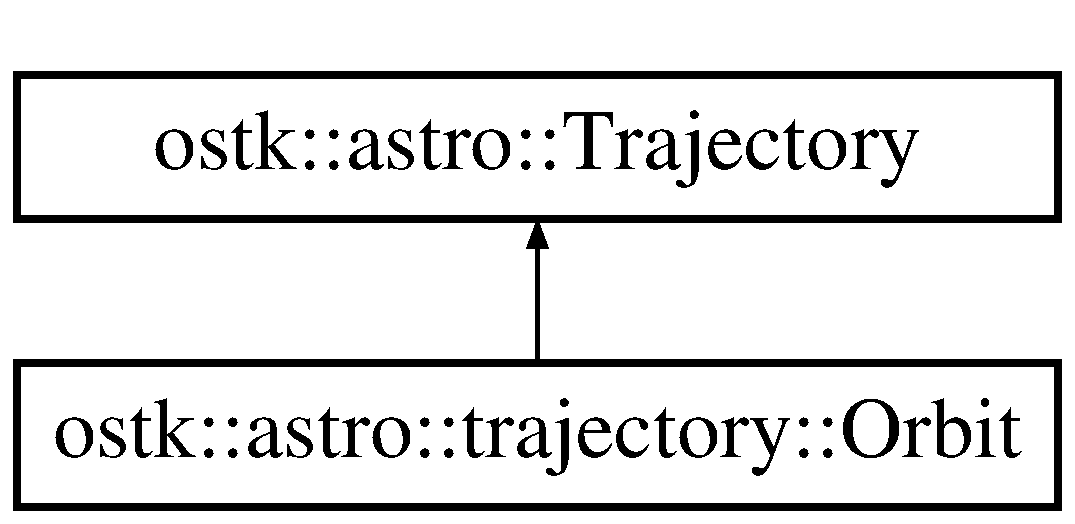
\includegraphics[height=2.000000cm]{classostk_1_1astro_1_1_trajectory}
\end{center}
\end{figure}
\subsection*{Public Member Functions}
\begin{DoxyCompactItemize}
\item 
\hyperlink{classostk_1_1astro_1_1_trajectory_a9333200bd6afed5aef4f5aad8a2a8e84}{Trajectory} (const \hyperlink{classostk_1_1astro_1_1trajectory_1_1_model}{Model} \&a\+Model)
\begin{DoxyCompactList}\small\item\em Constructor (model) \end{DoxyCompactList}\item 
\hyperlink{classostk_1_1astro_1_1_trajectory_a5bffa48518940b06d353988efdeb098a}{Trajectory} (const Array$<$ \hyperlink{classostk_1_1astro_1_1trajectory_1_1_state}{State} $>$ \&a\+State\+Array)
\begin{DoxyCompactList}\small\item\em Constructor (state array) \end{DoxyCompactList}\item 
\hyperlink{classostk_1_1astro_1_1_trajectory_a2a7642fa6183da49b5def83f63f08c42}{Trajectory} (const \hyperlink{classostk_1_1astro_1_1_trajectory}{Trajectory} \&a\+Trajectory)
\begin{DoxyCompactList}\small\item\em Copy constructor. \end{DoxyCompactList}\item 
\hyperlink{classostk_1_1astro_1_1_trajectory}{Trajectory} \& \hyperlink{classostk_1_1astro_1_1_trajectory_aa8229045bd7cf0696b8cd235cc3837a8}{operator=} (const \hyperlink{classostk_1_1astro_1_1_trajectory}{Trajectory} \&a\+Trajectory)
\begin{DoxyCompactList}\small\item\em Copy assignment operator. \end{DoxyCompactList}\item 
bool \hyperlink{classostk_1_1astro_1_1_trajectory_a13b1a0621195ed85aa3df0da5ae935f2}{operator==} (const \hyperlink{classostk_1_1astro_1_1_trajectory}{Trajectory} \&a\+Trajectory) const
\begin{DoxyCompactList}\small\item\em Equal to operator. \end{DoxyCompactList}\item 
bool \hyperlink{classostk_1_1astro_1_1_trajectory_abb524dcee260456d546f5e01ee9c228c}{operator!=} (const \hyperlink{classostk_1_1astro_1_1_trajectory}{Trajectory} \&a\+Trajectory) const
\begin{DoxyCompactList}\small\item\em Not equal to operator. \end{DoxyCompactList}\item 
bool \hyperlink{classostk_1_1astro_1_1_trajectory_ab0c02a9844e584b50da35df710b71e81}{is\+Defined} () const
\begin{DoxyCompactList}\small\item\em Check if trajectory is defined. \end{DoxyCompactList}\item 
const \hyperlink{classostk_1_1astro_1_1trajectory_1_1_model}{Model} \& \hyperlink{classostk_1_1astro_1_1_trajectory_a7a5e15ddb0b4e1a1546615840610252c}{access\+Model} () const
\begin{DoxyCompactList}\small\item\em \hyperlink{classostk_1_1astro_1_1_access}{Access} trajectory model. \end{DoxyCompactList}\item 
\hyperlink{classostk_1_1astro_1_1trajectory_1_1_state}{State} \hyperlink{classostk_1_1astro_1_1_trajectory_a0814d622d4bfb55cedb3d8eafd39f640}{get\+State\+At} (const Instant \&an\+Instant) const
\begin{DoxyCompactList}\small\item\em Get state at a given instant. \end{DoxyCompactList}\item 
Array$<$ \hyperlink{classostk_1_1astro_1_1trajectory_1_1_state}{State} $>$ \hyperlink{classostk_1_1astro_1_1_trajectory_a31f02515d567ac57c8d5e06d47da08a8}{get\+States\+At} (const Array$<$ Instant $>$ \&an\+Instant\+Array) const
\begin{DoxyCompactList}\small\item\em Get states at a given instants. \end{DoxyCompactList}\item 
virtual void \hyperlink{classostk_1_1astro_1_1_trajectory_aac11fb7c53f4cf970f52f681a75c5261}{print} (std\+::ostream \&an\+Output\+Stream, bool display\+Decorator=true) const
\begin{DoxyCompactList}\small\item\em Print trajectory to output stream. \end{DoxyCompactList}\end{DoxyCompactItemize}
\subsection*{Static Public Member Functions}
\begin{DoxyCompactItemize}
\item 
static \hyperlink{classostk_1_1astro_1_1_trajectory}{Trajectory} \hyperlink{classostk_1_1astro_1_1_trajectory_a87873d63cae80dff7e43c97dc9b3668f}{Undefined} ()
\begin{DoxyCompactList}\small\item\em Constructs an undefined trajectory. \end{DoxyCompactList}\item 
static \hyperlink{classostk_1_1astro_1_1_trajectory}{Trajectory} \hyperlink{classostk_1_1astro_1_1_trajectory_ae98d1466450030f73a83567c8cc1471a}{Position} (const physics\+::coord\+::\+Position \&a\+Position)
\begin{DoxyCompactList}\small\item\em Constructs a trajectory from a given position. \end{DoxyCompactList}\end{DoxyCompactItemize}
\subsection*{Friends}
\begin{DoxyCompactItemize}
\item 
std\+::ostream \& \hyperlink{classostk_1_1astro_1_1_trajectory_aef0327f0240dc2d71eca34dc287f88ea}{operator$<$$<$} (std\+::ostream \&an\+Output\+Stream, const \hyperlink{classostk_1_1astro_1_1_trajectory}{Trajectory} \&a\+Trajectory)
\begin{DoxyCompactList}\small\item\em Output stream operator. \end{DoxyCompactList}\end{DoxyCompactItemize}


\subsection{Detailed Description}
Path followed by an object through space as a function of time. 

https\+://en.wikipedia.\+org/wiki/\+Trajectory 

\subsection{Constructor \& Destructor Documentation}
\mbox{\Hypertarget{classostk_1_1astro_1_1_trajectory_a9333200bd6afed5aef4f5aad8a2a8e84}\label{classostk_1_1astro_1_1_trajectory_a9333200bd6afed5aef4f5aad8a2a8e84}} 
\index{ostk\+::astro\+::\+Trajectory@{ostk\+::astro\+::\+Trajectory}!Trajectory@{Trajectory}}
\index{Trajectory@{Trajectory}!ostk\+::astro\+::\+Trajectory@{ostk\+::astro\+::\+Trajectory}}
\subsubsection{\texorpdfstring{Trajectory()}{Trajectory()}\hspace{0.1cm}{\footnotesize\ttfamily [1/3]}}
{\footnotesize\ttfamily ostk\+::astro\+::\+Trajectory\+::\+Trajectory (\begin{DoxyParamCaption}\item[{const \hyperlink{classostk_1_1astro_1_1trajectory_1_1_model}{Model} \&}]{a\+Model }\end{DoxyParamCaption})}



Constructor (model) 


\begin{DoxyCode}
Tabulated model = \hyperlink{classostk_1_1astro_1_1trajectory_1_1models_1_1_tabulated_a81cf8ebea4354805ab69e732bfe73d77}{Tabulated::Load}(File::Path(Path::Parse(\textcolor{stringliteral}{"/path/to/trajectory.csv"}))) ;
\hyperlink{classostk_1_1astro_1_1_trajectory_a9333200bd6afed5aef4f5aad8a2a8e84}{Trajectory} trajectory = \{ model \} ;
\end{DoxyCode}



\begin{DoxyParams}[1]{Parameters}
\mbox{\tt in}  & {\em a\+Model} & A trajectory model \\
\hline
\end{DoxyParams}
\mbox{\Hypertarget{classostk_1_1astro_1_1_trajectory_a5bffa48518940b06d353988efdeb098a}\label{classostk_1_1astro_1_1_trajectory_a5bffa48518940b06d353988efdeb098a}} 
\index{ostk\+::astro\+::\+Trajectory@{ostk\+::astro\+::\+Trajectory}!Trajectory@{Trajectory}}
\index{Trajectory@{Trajectory}!ostk\+::astro\+::\+Trajectory@{ostk\+::astro\+::\+Trajectory}}
\subsubsection{\texorpdfstring{Trajectory()}{Trajectory()}\hspace{0.1cm}{\footnotesize\ttfamily [2/3]}}
{\footnotesize\ttfamily ostk\+::astro\+::\+Trajectory\+::\+Trajectory (\begin{DoxyParamCaption}\item[{const Array$<$ \hyperlink{classostk_1_1astro_1_1trajectory_1_1_state}{State} $>$ \&}]{a\+State\+Array }\end{DoxyParamCaption})}



Constructor (state array) 


\begin{DoxyCode}
Array<State> stateArray = \{ ... \} ;
\hyperlink{classostk_1_1astro_1_1_trajectory_a9333200bd6afed5aef4f5aad8a2a8e84}{Trajectory} trajectory = \{ stateArray \} ;
\end{DoxyCode}



\begin{DoxyParams}[1]{Parameters}
\mbox{\tt in}  & {\em a\+State\+Array} & An array of states \\
\hline
\end{DoxyParams}
\mbox{\Hypertarget{classostk_1_1astro_1_1_trajectory_a2a7642fa6183da49b5def83f63f08c42}\label{classostk_1_1astro_1_1_trajectory_a2a7642fa6183da49b5def83f63f08c42}} 
\index{ostk\+::astro\+::\+Trajectory@{ostk\+::astro\+::\+Trajectory}!Trajectory@{Trajectory}}
\index{Trajectory@{Trajectory}!ostk\+::astro\+::\+Trajectory@{ostk\+::astro\+::\+Trajectory}}
\subsubsection{\texorpdfstring{Trajectory()}{Trajectory()}\hspace{0.1cm}{\footnotesize\ttfamily [3/3]}}
{\footnotesize\ttfamily ostk\+::astro\+::\+Trajectory\+::\+Trajectory (\begin{DoxyParamCaption}\item[{const \hyperlink{classostk_1_1astro_1_1_trajectory}{Trajectory} \&}]{a\+Trajectory }\end{DoxyParamCaption})}



Copy constructor. 


\begin{DoxyParams}[1]{Parameters}
\mbox{\tt in}  & {\em a\+Trajectory} & A trajectory \\
\hline
\end{DoxyParams}


\subsection{Member Function Documentation}
\mbox{\Hypertarget{classostk_1_1astro_1_1_trajectory_a7a5e15ddb0b4e1a1546615840610252c}\label{classostk_1_1astro_1_1_trajectory_a7a5e15ddb0b4e1a1546615840610252c}} 
\index{ostk\+::astro\+::\+Trajectory@{ostk\+::astro\+::\+Trajectory}!access\+Model@{access\+Model}}
\index{access\+Model@{access\+Model}!ostk\+::astro\+::\+Trajectory@{ostk\+::astro\+::\+Trajectory}}
\subsubsection{\texorpdfstring{access\+Model()}{accessModel()}}
{\footnotesize\ttfamily const \hyperlink{classostk_1_1astro_1_1trajectory_1_1_model}{Model} \& ostk\+::astro\+::\+Trajectory\+::access\+Model (\begin{DoxyParamCaption}{ }\end{DoxyParamCaption}) const}



\hyperlink{classostk_1_1astro_1_1_access}{Access} trajectory model. 

\begin{DoxyReturn}{Returns}
Reference to trajectory model 
\end{DoxyReturn}
\mbox{\Hypertarget{classostk_1_1astro_1_1_trajectory_a0814d622d4bfb55cedb3d8eafd39f640}\label{classostk_1_1astro_1_1_trajectory_a0814d622d4bfb55cedb3d8eafd39f640}} 
\index{ostk\+::astro\+::\+Trajectory@{ostk\+::astro\+::\+Trajectory}!get\+State\+At@{get\+State\+At}}
\index{get\+State\+At@{get\+State\+At}!ostk\+::astro\+::\+Trajectory@{ostk\+::astro\+::\+Trajectory}}
\subsubsection{\texorpdfstring{get\+State\+At()}{getStateAt()}}
{\footnotesize\ttfamily \hyperlink{classostk_1_1astro_1_1trajectory_1_1_state}{State} ostk\+::astro\+::\+Trajectory\+::get\+State\+At (\begin{DoxyParamCaption}\item[{const Instant \&}]{an\+Instant }\end{DoxyParamCaption}) const}



Get state at a given instant. 


\begin{DoxyCode}
\hyperlink{classostk_1_1astro_1_1_trajectory_a9333200bd6afed5aef4f5aad8a2a8e84}{Trajectory} trajectory = \{ ... \} ;
Instant instant = \{ ... \} ;
State state = trajectory.getStateAt(instant) ;
\end{DoxyCode}



\begin{DoxyParams}[1]{Parameters}
\mbox{\tt in}  & {\em an\+Instant} & An instant \\
\hline
\end{DoxyParams}
\begin{DoxyReturn}{Returns}
State 
\end{DoxyReturn}
\mbox{\Hypertarget{classostk_1_1astro_1_1_trajectory_a31f02515d567ac57c8d5e06d47da08a8}\label{classostk_1_1astro_1_1_trajectory_a31f02515d567ac57c8d5e06d47da08a8}} 
\index{ostk\+::astro\+::\+Trajectory@{ostk\+::astro\+::\+Trajectory}!get\+States\+At@{get\+States\+At}}
\index{get\+States\+At@{get\+States\+At}!ostk\+::astro\+::\+Trajectory@{ostk\+::astro\+::\+Trajectory}}
\subsubsection{\texorpdfstring{get\+States\+At()}{getStatesAt()}}
{\footnotesize\ttfamily Array$<$ \hyperlink{classostk_1_1astro_1_1trajectory_1_1_state}{State} $>$ ostk\+::astro\+::\+Trajectory\+::get\+States\+At (\begin{DoxyParamCaption}\item[{const Array$<$ Instant $>$ \&}]{an\+Instant\+Array }\end{DoxyParamCaption}) const}



Get states at a given instants. 


\begin{DoxyCode}
\hyperlink{classostk_1_1astro_1_1_trajectory_a9333200bd6afed5aef4f5aad8a2a8e84}{Trajectory} trajectory = \{ ... \} ;
Array<Instant> instants = \{ ... \} ;
Array<State> state = trajectory.getStatesAt(instants) ;
\end{DoxyCode}



\begin{DoxyParams}[1]{Parameters}
\mbox{\tt in}  & {\em an\+Instant\+Array} & An array of instants \\
\hline
\end{DoxyParams}
\begin{DoxyReturn}{Returns}
Array of states 
\end{DoxyReturn}
\mbox{\Hypertarget{classostk_1_1astro_1_1_trajectory_ab0c02a9844e584b50da35df710b71e81}\label{classostk_1_1astro_1_1_trajectory_ab0c02a9844e584b50da35df710b71e81}} 
\index{ostk\+::astro\+::\+Trajectory@{ostk\+::astro\+::\+Trajectory}!is\+Defined@{is\+Defined}}
\index{is\+Defined@{is\+Defined}!ostk\+::astro\+::\+Trajectory@{ostk\+::astro\+::\+Trajectory}}
\subsubsection{\texorpdfstring{is\+Defined()}{isDefined()}}
{\footnotesize\ttfamily bool ostk\+::astro\+::\+Trajectory\+::is\+Defined (\begin{DoxyParamCaption}{ }\end{DoxyParamCaption}) const}



Check if trajectory is defined. 


\begin{DoxyCode}
\hyperlink{classostk_1_1astro_1_1_trajectory_a9333200bd6afed5aef4f5aad8a2a8e84}{Trajectory}(...).isDefined() ;
\end{DoxyCode}


\begin{DoxyReturn}{Returns}
True if trajectory is defined 
\end{DoxyReturn}
\mbox{\Hypertarget{classostk_1_1astro_1_1_trajectory_abb524dcee260456d546f5e01ee9c228c}\label{classostk_1_1astro_1_1_trajectory_abb524dcee260456d546f5e01ee9c228c}} 
\index{ostk\+::astro\+::\+Trajectory@{ostk\+::astro\+::\+Trajectory}!operator"!=@{operator"!=}}
\index{operator"!=@{operator"!=}!ostk\+::astro\+::\+Trajectory@{ostk\+::astro\+::\+Trajectory}}
\subsubsection{\texorpdfstring{operator"!=()}{operator!=()}}
{\footnotesize\ttfamily bool ostk\+::astro\+::\+Trajectory\+::operator!= (\begin{DoxyParamCaption}\item[{const \hyperlink{classostk_1_1astro_1_1_trajectory}{Trajectory} \&}]{a\+Trajectory }\end{DoxyParamCaption}) const}



Not equal to operator. 


\begin{DoxyCode}
\hyperlink{classostk_1_1astro_1_1_trajectory_a9333200bd6afed5aef4f5aad8a2a8e84}{Trajectory}(...) != \hyperlink{classostk_1_1astro_1_1_trajectory_a9333200bd6afed5aef4f5aad8a2a8e84}{Trajectory}(...) ;
\end{DoxyCode}



\begin{DoxyParams}[1]{Parameters}
\mbox{\tt in}  & {\em a\+Trajectory} & A trajectory \\
\hline
\end{DoxyParams}
\begin{DoxyReturn}{Returns}
True if trajectories are not equal 
\end{DoxyReturn}
\mbox{\Hypertarget{classostk_1_1astro_1_1_trajectory_aa8229045bd7cf0696b8cd235cc3837a8}\label{classostk_1_1astro_1_1_trajectory_aa8229045bd7cf0696b8cd235cc3837a8}} 
\index{ostk\+::astro\+::\+Trajectory@{ostk\+::astro\+::\+Trajectory}!operator=@{operator=}}
\index{operator=@{operator=}!ostk\+::astro\+::\+Trajectory@{ostk\+::astro\+::\+Trajectory}}
\subsubsection{\texorpdfstring{operator=()}{operator=()}}
{\footnotesize\ttfamily \hyperlink{classostk_1_1astro_1_1_trajectory}{Trajectory} \& ostk\+::astro\+::\+Trajectory\+::operator= (\begin{DoxyParamCaption}\item[{const \hyperlink{classostk_1_1astro_1_1_trajectory}{Trajectory} \&}]{a\+Trajectory }\end{DoxyParamCaption})}



Copy assignment operator. 

\mbox{\Hypertarget{classostk_1_1astro_1_1_trajectory_a13b1a0621195ed85aa3df0da5ae935f2}\label{classostk_1_1astro_1_1_trajectory_a13b1a0621195ed85aa3df0da5ae935f2}} 
\index{ostk\+::astro\+::\+Trajectory@{ostk\+::astro\+::\+Trajectory}!operator==@{operator==}}
\index{operator==@{operator==}!ostk\+::astro\+::\+Trajectory@{ostk\+::astro\+::\+Trajectory}}
\subsubsection{\texorpdfstring{operator==()}{operator==()}}
{\footnotesize\ttfamily bool ostk\+::astro\+::\+Trajectory\+::operator== (\begin{DoxyParamCaption}\item[{const \hyperlink{classostk_1_1astro_1_1_trajectory}{Trajectory} \&}]{a\+Trajectory }\end{DoxyParamCaption}) const}



Equal to operator. 


\begin{DoxyCode}
\hyperlink{classostk_1_1astro_1_1_trajectory_a9333200bd6afed5aef4f5aad8a2a8e84}{Trajectory}(...) == \hyperlink{classostk_1_1astro_1_1_trajectory_a9333200bd6afed5aef4f5aad8a2a8e84}{Trajectory}(...) ;
\end{DoxyCode}



\begin{DoxyParams}[1]{Parameters}
\mbox{\tt in}  & {\em a\+Trajectory} & A trajectory \\
\hline
\end{DoxyParams}
\begin{DoxyReturn}{Returns}
True if trajectories are equal 
\end{DoxyReturn}
\mbox{\Hypertarget{classostk_1_1astro_1_1_trajectory_ae98d1466450030f73a83567c8cc1471a}\label{classostk_1_1astro_1_1_trajectory_ae98d1466450030f73a83567c8cc1471a}} 
\index{ostk\+::astro\+::\+Trajectory@{ostk\+::astro\+::\+Trajectory}!Position@{Position}}
\index{Position@{Position}!ostk\+::astro\+::\+Trajectory@{ostk\+::astro\+::\+Trajectory}}
\subsubsection{\texorpdfstring{Position()}{Position()}}
{\footnotesize\ttfamily \hyperlink{classostk_1_1astro_1_1_trajectory}{Trajectory} ostk\+::astro\+::\+Trajectory\+::\+Position (\begin{DoxyParamCaption}\item[{const physics\+::coord\+::\+Position \&}]{a\+Position }\end{DoxyParamCaption})\hspace{0.3cm}{\ttfamily [static]}}



Constructs a trajectory from a given position. 


\begin{DoxyCode}
\hyperlink{classostk_1_1astro_1_1_trajectory_ae98d1466450030f73a83567c8cc1471a}{Position} position = Position::Meters(\{ 0.0, 0.0, 0.0 \}, Frame::GCRF()) ;
\hyperlink{classostk_1_1astro_1_1_trajectory_a9333200bd6afed5aef4f5aad8a2a8e84}{Trajectory} trajectory = \hyperlink{classostk_1_1astro_1_1_trajectory_ae98d1466450030f73a83567c8cc1471a}{Trajectory::Position}(position) ;
\end{DoxyCode}



\begin{DoxyParams}[1]{Parameters}
\mbox{\tt in}  & {\em a\+Position} & A position \\
\hline
\end{DoxyParams}
\begin{DoxyReturn}{Returns}
Static trajectory 
\end{DoxyReturn}
\mbox{\Hypertarget{classostk_1_1astro_1_1_trajectory_aac11fb7c53f4cf970f52f681a75c5261}\label{classostk_1_1astro_1_1_trajectory_aac11fb7c53f4cf970f52f681a75c5261}} 
\index{ostk\+::astro\+::\+Trajectory@{ostk\+::astro\+::\+Trajectory}!print@{print}}
\index{print@{print}!ostk\+::astro\+::\+Trajectory@{ostk\+::astro\+::\+Trajectory}}
\subsubsection{\texorpdfstring{print()}{print()}}
{\footnotesize\ttfamily void ostk\+::astro\+::\+Trajectory\+::print (\begin{DoxyParamCaption}\item[{std\+::ostream \&}]{an\+Output\+Stream,  }\item[{bool}]{display\+Decorator = {\ttfamily true} }\end{DoxyParamCaption}) const\hspace{0.3cm}{\ttfamily [virtual]}}



Print trajectory to output stream. 


\begin{DoxyCode}
\hyperlink{classostk_1_1astro_1_1_trajectory_a9333200bd6afed5aef4f5aad8a2a8e84}{Trajectory} trajectory = \{ ... \} ;
trajectory.print(std::cout, \textcolor{keyword}{true}) ;
\end{DoxyCode}



\begin{DoxyParams}[1]{Parameters}
\mbox{\tt in}  & {\em an\+Output\+Stream} & An output stream \\
\hline
\mbox{\tt in}  & {\em display\+Decorator} & If true, display decorator \\
\hline
\end{DoxyParams}


Reimplemented in \hyperlink{classostk_1_1astro_1_1trajectory_1_1_orbit_ae890e832785f84c3f03c1e103f952826}{ostk\+::astro\+::trajectory\+::\+Orbit}.

\mbox{\Hypertarget{classostk_1_1astro_1_1_trajectory_a87873d63cae80dff7e43c97dc9b3668f}\label{classostk_1_1astro_1_1_trajectory_a87873d63cae80dff7e43c97dc9b3668f}} 
\index{ostk\+::astro\+::\+Trajectory@{ostk\+::astro\+::\+Trajectory}!Undefined@{Undefined}}
\index{Undefined@{Undefined}!ostk\+::astro\+::\+Trajectory@{ostk\+::astro\+::\+Trajectory}}
\subsubsection{\texorpdfstring{Undefined()}{Undefined()}}
{\footnotesize\ttfamily \hyperlink{classostk_1_1astro_1_1_trajectory}{Trajectory} ostk\+::astro\+::\+Trajectory\+::\+Undefined (\begin{DoxyParamCaption}{ }\end{DoxyParamCaption})\hspace{0.3cm}{\ttfamily [static]}}



Constructs an undefined trajectory. 


\begin{DoxyCode}
\hyperlink{classostk_1_1astro_1_1_trajectory_a9333200bd6afed5aef4f5aad8a2a8e84}{Trajectory} trajectory = \hyperlink{classostk_1_1astro_1_1_trajectory_a87873d63cae80dff7e43c97dc9b3668f}{Trajectory::Undefined}() ; \textcolor{comment}{// Undefined}
\end{DoxyCode}


\begin{DoxyReturn}{Returns}
Undefined trajectory 
\end{DoxyReturn}


\subsection{Friends And Related Function Documentation}
\mbox{\Hypertarget{classostk_1_1astro_1_1_trajectory_aef0327f0240dc2d71eca34dc287f88ea}\label{classostk_1_1astro_1_1_trajectory_aef0327f0240dc2d71eca34dc287f88ea}} 
\index{ostk\+::astro\+::\+Trajectory@{ostk\+::astro\+::\+Trajectory}!operator$<$$<$@{operator$<$$<$}}
\index{operator$<$$<$@{operator$<$$<$}!ostk\+::astro\+::\+Trajectory@{ostk\+::astro\+::\+Trajectory}}
\subsubsection{\texorpdfstring{operator$<$$<$}{operator<<}}
{\footnotesize\ttfamily std\+::ostream\& operator$<$$<$ (\begin{DoxyParamCaption}\item[{std\+::ostream \&}]{an\+Output\+Stream,  }\item[{const \hyperlink{classostk_1_1astro_1_1_trajectory}{Trajectory} \&}]{a\+Trajectory }\end{DoxyParamCaption})\hspace{0.3cm}{\ttfamily [friend]}}



Output stream operator. 


\begin{DoxyCode}
std::cout << \hyperlink{classostk_1_1astro_1_1_trajectory_a9333200bd6afed5aef4f5aad8a2a8e84}{Trajectory}(...) ;
\end{DoxyCode}



\begin{DoxyParams}[1]{Parameters}
\mbox{\tt in}  & {\em an\+Output\+Stream} & An output stream \\
\hline
\mbox{\tt in}  & {\em a\+Trajectory} & A trajectory \\
\hline
\end{DoxyParams}
\begin{DoxyReturn}{Returns}
A reference to output stream 
\end{DoxyReturn}


The documentation for this class was generated from the following files\+:\begin{DoxyCompactItemize}
\item 
include/\+Open\+Space\+Toolkit/\+Astrodynamics/\hyperlink{_trajectory_8hpp}{Trajectory.\+hpp}\item 
src/\+Open\+Space\+Toolkit/\+Astrodynamics/\hyperlink{_trajectory_8cpp}{Trajectory.\+cpp}\end{DoxyCompactItemize}

\chapter{File Documentation}
\hypertarget{_c_o_n_t_r_i_b_u_t_i_n_g_8md}{}\section{C\+O\+N\+T\+R\+I\+B\+U\+T\+I\+N\+G.\+md File Reference}
\label{_c_o_n_t_r_i_b_u_t_i_n_g_8md}\index{C\+O\+N\+T\+R\+I\+B\+U\+T\+I\+N\+G.\+md@{C\+O\+N\+T\+R\+I\+B\+U\+T\+I\+N\+G.\+md}}

\hypertarget{_tutorial_8md}{}\section{docs/\+Tutorial.md File Reference}
\label{_tutorial_8md}\index{docs/\+Tutorial.\+md@{docs/\+Tutorial.\+md}}

\hypertarget{_access_8hpp}{}\section{include/\+Open\+Space\+Toolkit/\+Astrodynamics/\+Access.hpp File Reference}
\label{_access_8hpp}\index{include/\+Open\+Space\+Toolkit/\+Astrodynamics/\+Access.\+hpp@{include/\+Open\+Space\+Toolkit/\+Astrodynamics/\+Access.\+hpp}}
{\ttfamily \#include $<$Open\+Space\+Toolkit/\+Physics/\+Time/\+Interval.\+hpp$>$}\newline
{\ttfamily \#include $<$Open\+Space\+Toolkit/\+Physics/\+Time/\+Duration.\+hpp$>$}\newline
{\ttfamily \#include $<$Open\+Space\+Toolkit/\+Physics/\+Time/\+Instant.\+hpp$>$}\newline
{\ttfamily \#include $<$Open\+Space\+Toolkit/\+Core/\+Containers/\+Array.\+hpp$>$}\newline
{\ttfamily \#include $<$Open\+Space\+Toolkit/\+Core/\+Types/\+String.\+hpp$>$}\newline
\subsection*{Classes}
\begin{DoxyCompactItemize}
\item 
class \hyperlink{classostk_1_1astro_1_1_access}{ostk\+::astro\+::\+Access}
\begin{DoxyCompactList}\small\item\em Object-\/to-\/object visibility. \end{DoxyCompactList}\end{DoxyCompactItemize}
\subsection*{Namespaces}
\begin{DoxyCompactItemize}
\item 
 \hyperlink{namespaceostk}{ostk}
\item 
 \hyperlink{namespaceostk_1_1astro}{ostk\+::astro}
\end{DoxyCompactItemize}


\subsection{Detailed Description}
Open Space Toolkit ▸ Astrodynamics

\begin{DoxyAuthor}{Author}
Lucas Brémond \href{mailto:lucas@loftorbital.com}{\tt lucas@loftorbital.\+com}  Apache License 2.\+0 
\end{DoxyAuthor}

\hypertarget{_generator_8hpp}{}\section{include/\+Open\+Space\+Toolkit/\+Astrodynamics/\+Access/\+Generator.hpp File Reference}
\label{_generator_8hpp}\index{include/\+Open\+Space\+Toolkit/\+Astrodynamics/\+Access/\+Generator.\+hpp@{include/\+Open\+Space\+Toolkit/\+Astrodynamics/\+Access/\+Generator.\+hpp}}
{\ttfamily \#include $<$Open\+Space\+Toolkit/\+Astrodynamics/\+Access.\+hpp$>$}\newline
{\ttfamily \#include $<$Open\+Space\+Toolkit/\+Astrodynamics/\+Trajectory.\+hpp$>$}\newline
{\ttfamily \#include $<$Open\+Space\+Toolkit/\+Physics/\+Environment.\+hpp$>$}\newline
{\ttfamily \#include $<$Open\+Space\+Toolkit/\+Physics/\+Coordinate/\+Spherical/\+A\+E\+R.\+hpp$>$}\newline
{\ttfamily \#include $<$Open\+Space\+Toolkit/\+Physics/\+Time/\+Interval.\+hpp$>$}\newline
{\ttfamily \#include $<$Open\+Space\+Toolkit/\+Physics/\+Time/\+Instant.\+hpp$>$}\newline
{\ttfamily \#include $<$Open\+Space\+Toolkit/\+Physics/\+Units/\+Derived/\+Angle.\+hpp$>$}\newline
{\ttfamily \#include $<$Open\+Space\+Toolkit/\+Physics/\+Units/\+Length.\+hpp$>$}\newline
{\ttfamily \#include $<$Open\+Space\+Toolkit/\+Mathematics/\+Objects/\+Interval.\+hpp$>$}\newline
{\ttfamily \#include $<$Open\+Space\+Toolkit/\+Core/\+Containers/\+Array.\+hpp$>$}\newline
{\ttfamily \#include $<$Open\+Space\+Toolkit/\+Core/\+Types/\+Real.\+hpp$>$}\newline
\subsection*{Classes}
\begin{DoxyCompactItemize}
\item 
class \hyperlink{classostk_1_1astro_1_1access_1_1_generator}{ostk\+::astro\+::access\+::\+Generator}
\end{DoxyCompactItemize}
\subsection*{Namespaces}
\begin{DoxyCompactItemize}
\item 
 \hyperlink{namespaceostk}{ostk}
\item 
 \hyperlink{namespaceostk_1_1astro}{ostk\+::astro}
\item 
 \hyperlink{namespaceostk_1_1astro_1_1access}{ostk\+::astro\+::access}
\end{DoxyCompactItemize}


\subsection{Detailed Description}
Open Space Toolkit ▸ Astrodynamics

\begin{DoxyAuthor}{Author}
Lucas Brémond \href{mailto:lucas@loftorbital.com}{\tt lucas@loftorbital.\+com}  Apache License 2.\+0 
\end{DoxyAuthor}

\hypertarget{_flight_8hpp}{}\section{include/\+Library/\+Astrodynamics/\+Flight.hpp File Reference}
\label{_flight_8hpp}\index{include/\+Library/\+Astrodynamics/\+Flight.\+hpp@{include/\+Library/\+Astrodynamics/\+Flight.\+hpp}}
{\ttfamily \#include $<$Library/\+Astrodynamics/\+Flight/\+Profile/\+State.\+hpp$>$}\newline
{\ttfamily \#include $<$Library/\+Astrodynamics/\+Flight/\+Profile.\+hpp$>$}\newline
\subsection*{Namespaces}
\begin{DoxyCompactItemize}
\item 
 \hyperlink{namespacelibrary}{library}
\item 
 \hyperlink{namespacelibrary_1_1astro}{library\+::astro}
\end{DoxyCompactItemize}


\subsection{Detailed Description}
Library/\+Astrodynamics

\begin{DoxyAuthor}{Author}
Lucas Brémond \href{mailto:lucas@loftorbital.com}{\tt lucas@loftorbital.\+com}  Apache License 2.\+0 
\end{DoxyAuthor}

\hypertarget{_profile_8hpp}{}\section{include/\+Open\+Space\+Toolkit/\+Astrodynamics/\+Flight/\+Profile.hpp File Reference}
\label{_profile_8hpp}\index{include/\+Open\+Space\+Toolkit/\+Astrodynamics/\+Flight/\+Profile.\+hpp@{include/\+Open\+Space\+Toolkit/\+Astrodynamics/\+Flight/\+Profile.\+hpp}}
{\ttfamily \#include $<$Open\+Space\+Toolkit/\+Astrodynamics/\+Flight/\+Profile/\+State.\+hpp$>$}\newline
{\ttfamily \#include $<$Open\+Space\+Toolkit/\+Astrodynamics/\+Trajectory/\+Orbit.\+hpp$>$}\newline
{\ttfamily \#include $<$Open\+Space\+Toolkit/\+Astrodynamics/\+Trajectory.\+hpp$>$}\newline
{\ttfamily \#include $<$Open\+Space\+Toolkit/\+Physics/\+Coordinate/\+Frame/\+Providers/\+Dynamic.\+hpp$>$}\newline
{\ttfamily \#include $<$Open\+Space\+Toolkit/\+Physics/\+Coordinate/\+Axes.\+hpp$>$}\newline
{\ttfamily \#include $<$Open\+Space\+Toolkit/\+Physics/\+Time/\+Interval.\+hpp$>$}\newline
{\ttfamily \#include $<$Open\+Space\+Toolkit/\+Physics/\+Time/\+Duration.\+hpp$>$}\newline
{\ttfamily \#include $<$Open\+Space\+Toolkit/\+Physics/\+Time/\+Instant.\+hpp$>$}\newline
{\ttfamily \#include $<$Open\+Space\+Toolkit/\+Mathematics/\+Geometry/3\+D/\+Transformations/\+Rotations/\+Rotation\+Matrix.\+hpp$>$}\newline
{\ttfamily \#include $<$Open\+Space\+Toolkit/\+Mathematics/\+Objects/\+Vector.\+hpp$>$}\newline
{\ttfamily \#include $<$Open\+Space\+Toolkit/\+Core/\+Containers/\+Array.\+hpp$>$}\newline
{\ttfamily \#include $<$Open\+Space\+Toolkit/\+Core/\+Types/\+String.\+hpp$>$}\newline
{\ttfamily \#include $<$Open\+Space\+Toolkit/\+Core/\+Types/\+Shared.\+hpp$>$}\newline
\subsection*{Classes}
\begin{DoxyCompactItemize}
\item 
class \hyperlink{classostk_1_1astro_1_1flight_1_1_profile}{ostk\+::astro\+::flight\+::\+Profile}
\begin{DoxyCompactList}\small\item\em Spacecraft flight profile. \end{DoxyCompactList}\end{DoxyCompactItemize}
\subsection*{Namespaces}
\begin{DoxyCompactItemize}
\item 
 \hyperlink{namespaceostk}{ostk}
\item 
 \hyperlink{namespaceostk_1_1astro}{ostk\+::astro}
\item 
 \hyperlink{namespaceostk_1_1astro_1_1flight}{ostk\+::astro\+::flight}
\end{DoxyCompactItemize}
\subsection*{Typedefs}
\begin{DoxyCompactItemize}
\item 
using \hyperlink{namespaceostk_1_1astro_1_1flight_a30fb17f0f77e97e4d6bb5567218816bd}{ostk\+::astro\+::flight\+::\+Dynamic\+Provider} = ostk\+::physics\+::coord\+::frame\+::provider\+::\+Dynamic
\end{DoxyCompactItemize}


\subsection{Detailed Description}
Open Space Toolkit ▸ Astrodynamics

\begin{DoxyAuthor}{Author}
Lucas Brémond \href{mailto:lucas@loftorbital.com}{\tt lucas@loftorbital.\+com}  Apache License 2.\+0 
\end{DoxyAuthor}

\hypertarget{_flight_2_profile_2_state_8hpp}{}\section{include/\+Library/\+Astrodynamics/\+Flight/\+Profile/\+State.hpp File Reference}
\label{_flight_2_profile_2_state_8hpp}\index{include/\+Library/\+Astrodynamics/\+Flight/\+Profile/\+State.\+hpp@{include/\+Library/\+Astrodynamics/\+Flight/\+Profile/\+State.\+hpp}}
{\ttfamily \#include $<$Library/\+Physics/\+Coordinate/\+Frame.\+hpp$>$}\newline
{\ttfamily \#include $<$Library/\+Physics/\+Time/\+Instant.\+hpp$>$}\newline
{\ttfamily \#include $<$Library/\+Mathematics/\+Geometry/3\+D/\+Transformations/\+Rotations/\+Rotation\+Matrix.\+hpp$>$}\newline
{\ttfamily \#include $<$Library/\+Mathematics/\+Objects/\+Vector.\+hpp$>$}\newline
{\ttfamily \#include $<$Library/\+Core/\+Types/\+Shared.\+hpp$>$}\newline
\subsection*{Classes}
\begin{DoxyCompactItemize}
\item 
class \hyperlink{classlibrary_1_1astro_1_1flight_1_1profile_1_1_state}{library\+::astro\+::flight\+::profile\+::\+State}
\begin{DoxyCompactList}\small\item\em Spacecraft flight profile state. \end{DoxyCompactList}\end{DoxyCompactItemize}
\subsection*{Namespaces}
\begin{DoxyCompactItemize}
\item 
 \hyperlink{namespacelibrary}{library}
\item 
 \hyperlink{namespacelibrary_1_1astro}{library\+::astro}
\item 
 \hyperlink{namespacelibrary_1_1astro_1_1flight}{library\+::astro\+::flight}
\item 
 \hyperlink{namespacelibrary_1_1astro_1_1flight_1_1profile}{library\+::astro\+::flight\+::profile}
\end{DoxyCompactItemize}


\subsection{Detailed Description}
Library/\+Astrodynamics

\begin{DoxyAuthor}{Author}
Lucas Brémond \href{mailto:lucas@loftorbital.com}{\tt lucas@loftorbital.\+com}  T\+BD 
\end{DoxyAuthor}

\hypertarget{_trajectory_2_state_8hpp}{}\section{include/\+Open\+Space\+Toolkit/\+Astrodynamics/\+Trajectory/\+State.hpp File Reference}
\label{_trajectory_2_state_8hpp}\index{include/\+Open\+Space\+Toolkit/\+Astrodynamics/\+Trajectory/\+State.\+hpp@{include/\+Open\+Space\+Toolkit/\+Astrodynamics/\+Trajectory/\+State.\+hpp}}
{\ttfamily \#include $<$Open\+Space\+Toolkit/\+Physics/\+Coordinate/\+Frame.\+hpp$>$}\newline
{\ttfamily \#include $<$Open\+Space\+Toolkit/\+Physics/\+Coordinate/\+Velocity.\+hpp$>$}\newline
{\ttfamily \#include $<$Open\+Space\+Toolkit/\+Physics/\+Coordinate/\+Position.\+hpp$>$}\newline
{\ttfamily \#include $<$Open\+Space\+Toolkit/\+Physics/\+Time/\+Instant.\+hpp$>$}\newline
{\ttfamily \#include $<$Open\+Space\+Toolkit/\+Core/\+Types/\+Shared.\+hpp$>$}\newline
\subsection*{Classes}
\begin{DoxyCompactItemize}
\item 
class \hyperlink{classostk_1_1astro_1_1trajectory_1_1_state}{ostk\+::astro\+::trajectory\+::\+State}
\begin{DoxyCompactList}\small\item\em \hyperlink{classostk_1_1astro_1_1_trajectory}{Trajectory} state. \end{DoxyCompactList}\end{DoxyCompactItemize}
\subsection*{Namespaces}
\begin{DoxyCompactItemize}
\item 
 \hyperlink{namespaceostk}{ostk}
\item 
 \hyperlink{namespaceostk_1_1astro}{ostk\+::astro}
\item 
 \hyperlink{namespaceostk_1_1astro_1_1trajectory}{ostk\+::astro\+::trajectory}
\end{DoxyCompactItemize}


\subsection{Detailed Description}
Open Space Toolkit ▸ Astrodynamics

\begin{DoxyAuthor}{Author}
Lucas Brémond \href{mailto:lucas@loftorbital.com}{\tt lucas@loftorbital.\+com}  Apache License 2.\+0 
\end{DoxyAuthor}

\hypertarget{_trajectory_8hpp}{}\section{include/\+Library/\+Astrodynamics/\+Trajectory.hpp File Reference}
\label{_trajectory_8hpp}\index{include/\+Library/\+Astrodynamics/\+Trajectory.\+hpp@{include/\+Library/\+Astrodynamics/\+Trajectory.\+hpp}}
{\ttfamily \#include $<$Library/\+Astrodynamics/\+Trajectory/\+State.\+hpp$>$}\newline
{\ttfamily \#include $<$Library/\+Astrodynamics/\+Trajectory/\+Model.\+hpp$>$}\newline
{\ttfamily \#include $<$Library/\+Physics/\+Coordinate/\+Position.\+hpp$>$}\newline
{\ttfamily \#include $<$Library/\+Physics/\+Time/\+Interval.\+hpp$>$}\newline
{\ttfamily \#include $<$Library/\+Physics/\+Time/\+Instant.\+hpp$>$}\newline
{\ttfamily \#include $<$Library/\+Core/\+Containers/\+Array.\+hpp$>$}\newline
{\ttfamily \#include $<$Library/\+Core/\+Types/\+String.\+hpp$>$}\newline
{\ttfamily \#include $<$Library/\+Core/\+Types/\+Index.\+hpp$>$}\newline
{\ttfamily \#include $<$Library/\+Core/\+Types/\+Unique.\+hpp$>$}\newline
\subsection*{Classes}
\begin{DoxyCompactItemize}
\item 
class \hyperlink{classlibrary_1_1astro_1_1_trajectory}{library\+::astro\+::\+Trajectory}
\begin{DoxyCompactList}\small\item\em Path followed by an object through space as a function of time. \end{DoxyCompactList}\end{DoxyCompactItemize}
\subsection*{Namespaces}
\begin{DoxyCompactItemize}
\item 
 \hyperlink{namespacelibrary}{library}
\item 
 \hyperlink{namespacelibrary_1_1astro}{library\+::astro}
\end{DoxyCompactItemize}


\subsection{Detailed Description}
Library/\+Astrodynamics

\begin{DoxyAuthor}{Author}
Lucas Brémond \href{mailto:lucas@loftorbital.com}{\tt lucas@loftorbital.\+com}  T\+BD 
\end{DoxyAuthor}

\hypertarget{_model_8hpp}{}\section{include/\+Library/\+Astrodynamics/\+Trajectory/\+Orbit/\+Model.hpp File Reference}
\label{_model_8hpp}\index{include/\+Library/\+Astrodynamics/\+Trajectory/\+Orbit/\+Model.\+hpp@{include/\+Library/\+Astrodynamics/\+Trajectory/\+Orbit/\+Model.\+hpp}}
{\ttfamily \#include $<$Library/\+Core/\+Types/\+String.\+hpp$>$}\newline
{\ttfamily \#include $<$Library/\+Core/\+Types/\+Real.\+hpp$>$}\newline
\subsection*{Classes}
\begin{DoxyCompactItemize}
\item 
class \hyperlink{classlibrary_1_1astro_1_1_model}{library\+::astro\+::\+Model}
\end{DoxyCompactItemize}
\subsection*{Namespaces}
\begin{DoxyCompactItemize}
\item 
 \hyperlink{namespacelibrary}{library}
\item 
 \hyperlink{namespacelibrary_1_1astro}{library\+::astro}
\end{DoxyCompactItemize}


\subsection{Detailed Description}
Library/\+Astrodynamics

\begin{DoxyAuthor}{Author}
Lucas Brémond \href{mailto:lucas@loftorbital.com}{\tt lucas@loftorbital.\+com}  T\+BD 
\end{DoxyAuthor}

\hypertarget{_orbit_2_model_8hpp}{}\section{include/\+Library/\+Astrodynamics/\+Trajectory/\+Orbit/\+Model.hpp File Reference}
\label{_orbit_2_model_8hpp}\index{include/\+Library/\+Astrodynamics/\+Trajectory/\+Orbit/\+Model.\+hpp@{include/\+Library/\+Astrodynamics/\+Trajectory/\+Orbit/\+Model.\+hpp}}
{\ttfamily \#include $<$Library/\+Astrodynamics/\+Trajectory/\+State.\+hpp$>$}\newline
{\ttfamily \#include $<$Library/\+Astrodynamics/\+Trajectory/\+Model.\+hpp$>$}\newline
{\ttfamily \#include $<$Library/\+Physics/\+Time/\+Instant.\+hpp$>$}\newline
{\ttfamily \#include $<$Library/\+Core/\+Types/\+Integer.\+hpp$>$}\newline
\subsection*{Classes}
\begin{DoxyCompactItemize}
\item 
class \hyperlink{classlibrary_1_1astro_1_1trajectory_1_1orbit_1_1_model}{library\+::astro\+::trajectory\+::orbit\+::\+Model}
\end{DoxyCompactItemize}
\subsection*{Namespaces}
\begin{DoxyCompactItemize}
\item 
 \hyperlink{namespacelibrary}{library}
\item 
 \hyperlink{namespacelibrary_1_1astro}{library\+::astro}
\item 
 \hyperlink{namespacelibrary_1_1astro_1_1trajectory}{library\+::astro\+::trajectory}
\item 
 \hyperlink{namespacelibrary_1_1astro_1_1trajectory_1_1orbit}{library\+::astro\+::trajectory\+::orbit}
\end{DoxyCompactItemize}


\subsection{Detailed Description}
Library/\+Astrodynamics

\begin{DoxyAuthor}{Author}
Lucas Brémond \href{mailto:lucas@loftorbital.com}{\tt lucas@loftorbital.\+com}  Apache License 2.\+0 
\end{DoxyAuthor}

\hypertarget{_static_8hpp}{}\section{include/\+Library/\+Astrodynamics/\+Trajectory/\+Models/\+Static.hpp File Reference}
\label{_static_8hpp}\index{include/\+Library/\+Astrodynamics/\+Trajectory/\+Models/\+Static.\+hpp@{include/\+Library/\+Astrodynamics/\+Trajectory/\+Models/\+Static.\+hpp}}
{\ttfamily \#include $<$Library/\+Astrodynamics/\+Trajectory/\+State.\+hpp$>$}\newline
{\ttfamily \#include $<$Library/\+Astrodynamics/\+Trajectory/\+Model.\+hpp$>$}\newline
{\ttfamily \#include $<$Library/\+Physics/\+Time/\+Interval.\+hpp$>$}\newline
{\ttfamily \#include $<$Library/\+Physics/\+Time/\+Instant.\+hpp$>$}\newline
\subsection*{Classes}
\begin{DoxyCompactItemize}
\item 
class \hyperlink{classlibrary_1_1astro_1_1trajectory_1_1models_1_1_static}{library\+::astro\+::trajectory\+::models\+::\+Static}
\begin{DoxyCompactList}\small\item\em \hyperlink{classlibrary_1_1astro_1_1trajectory_1_1models_1_1_static}{Static} trajectory model. \end{DoxyCompactList}\end{DoxyCompactItemize}
\subsection*{Namespaces}
\begin{DoxyCompactItemize}
\item 
 \hyperlink{namespacelibrary}{library}
\item 
 \hyperlink{namespacelibrary_1_1astro}{library\+::astro}
\item 
 \hyperlink{namespacelibrary_1_1astro_1_1trajectory}{library\+::astro\+::trajectory}
\item 
 \hyperlink{namespacelibrary_1_1astro_1_1trajectory_1_1models}{library\+::astro\+::trajectory\+::models}
\end{DoxyCompactItemize}


\subsection{Detailed Description}
Library/\+Astrodynamics

\begin{DoxyAuthor}{Author}
Lucas Brémond \href{mailto:lucas@loftorbital.com}{\tt lucas@loftorbital.\+com}  T\+BD 
\end{DoxyAuthor}

\hypertarget{_models_2_tabulated_8hpp}{}\section{include/\+Library/\+Astrodynamics/\+Trajectory/\+Models/\+Tabulated.hpp File Reference}
\label{_models_2_tabulated_8hpp}\index{include/\+Library/\+Astrodynamics/\+Trajectory/\+Models/\+Tabulated.\+hpp@{include/\+Library/\+Astrodynamics/\+Trajectory/\+Models/\+Tabulated.\+hpp}}
{\ttfamily \#include $<$Library/\+Astrodynamics/\+Trajectory/\+State.\+hpp$>$}\newline
{\ttfamily \#include $<$Library/\+Astrodynamics/\+Trajectory/\+Model.\+hpp$>$}\newline
{\ttfamily \#include $<$Library/\+Physics/\+Time/\+Interval.\+hpp$>$}\newline
{\ttfamily \#include $<$Library/\+Physics/\+Time/\+Instant.\+hpp$>$}\newline
{\ttfamily \#include $<$Library/\+Core/\+File\+System/\+File.\+hpp$>$}\newline
{\ttfamily \#include $<$Library/\+Core/\+Containers/\+Array.\+hpp$>$}\newline
{\ttfamily \#include $<$Library/\+Core/\+Containers/\+Pair.\+hpp$>$}\newline
{\ttfamily \#include $<$Library/\+Core/\+Types/\+Index.\+hpp$>$}\newline
\subsection*{Classes}
\begin{DoxyCompactItemize}
\item 
class \hyperlink{classlibrary_1_1astro_1_1trajectory_1_1models_1_1_tabulated}{library\+::astro\+::trajectory\+::models\+::\+Tabulated}
\begin{DoxyCompactList}\small\item\em \hyperlink{classlibrary_1_1astro_1_1trajectory_1_1models_1_1_tabulated}{Tabulated} trajectory model. \end{DoxyCompactList}\end{DoxyCompactItemize}
\subsection*{Namespaces}
\begin{DoxyCompactItemize}
\item 
 \hyperlink{namespacelibrary}{library}
\item 
 \hyperlink{namespacelibrary_1_1astro}{library\+::astro}
\item 
 \hyperlink{namespacelibrary_1_1astro_1_1trajectory}{library\+::astro\+::trajectory}
\item 
 \hyperlink{namespacelibrary_1_1astro_1_1trajectory_1_1models}{library\+::astro\+::trajectory\+::models}
\end{DoxyCompactItemize}


\subsection{Detailed Description}
Library/\+Astrodynamics

\begin{DoxyAuthor}{Author}
Lucas Brémond \href{mailto:lucas@loftorbital.com}{\tt lucas@loftorbital.\+com}  Apache License 2.\+0 
\end{DoxyAuthor}

\hypertarget{_orbit_2_models_2_tabulated_8hpp}{}\section{include/\+Open\+Space\+Toolkit/\+Astrodynamics/\+Trajectory/\+Orbit/\+Models/\+Tabulated.hpp File Reference}
\label{_orbit_2_models_2_tabulated_8hpp}\index{include/\+Open\+Space\+Toolkit/\+Astrodynamics/\+Trajectory/\+Orbit/\+Models/\+Tabulated.\+hpp@{include/\+Open\+Space\+Toolkit/\+Astrodynamics/\+Trajectory/\+Orbit/\+Models/\+Tabulated.\+hpp}}
{\ttfamily \#include $<$Open\+Space\+Toolkit/\+Astrodynamics/\+Trajectory/\+Orbit/\+Model.\+hpp$>$}\newline
{\ttfamily \#include $<$Open\+Space\+Toolkit/\+Astrodynamics/\+Trajectory/\+Models/\+Tabulated.\+hpp$>$}\newline
{\ttfamily \#include $<$Open\+Space\+Toolkit/\+Astrodynamics/\+Trajectory/\+State.\+hpp$>$}\newline
{\ttfamily \#include $<$Open\+Space\+Toolkit/\+Astrodynamics/\+Trajectory/\+Model.\+hpp$>$}\newline
{\ttfamily \#include $<$Open\+Space\+Toolkit/\+Physics/\+Time/\+Instant.\+hpp$>$}\newline
{\ttfamily \#include $<$Open\+Space\+Toolkit/\+Core/\+Containers/\+Array.\+hpp$>$}\newline
{\ttfamily \#include $<$Open\+Space\+Toolkit/\+Core/\+Types/\+Integer.\+hpp$>$}\newline
\subsection*{Classes}
\begin{DoxyCompactItemize}
\item 
class \hyperlink{classostk_1_1astro_1_1trajectory_1_1orbit_1_1models_1_1_tabulated}{ostk\+::astro\+::trajectory\+::orbit\+::models\+::\+Tabulated}
\end{DoxyCompactItemize}
\subsection*{Namespaces}
\begin{DoxyCompactItemize}
\item 
 \hyperlink{namespaceostk}{ostk}
\item 
 \hyperlink{namespaceostk_1_1astro}{ostk\+::astro}
\item 
 \hyperlink{namespaceostk_1_1astro_1_1trajectory}{ostk\+::astro\+::trajectory}
\item 
 \hyperlink{namespaceostk_1_1astro_1_1trajectory_1_1orbit}{ostk\+::astro\+::trajectory\+::orbit}
\item 
 \hyperlink{namespaceostk_1_1astro_1_1trajectory_1_1orbit_1_1models}{ostk\+::astro\+::trajectory\+::orbit\+::models}
\end{DoxyCompactItemize}


\subsection{Detailed Description}
Open Space Toolkit ▸ Astrodynamics

\begin{DoxyAuthor}{Author}
Lucas Brémond \href{mailto:lucas@loftorbital.com}{\tt lucas@loftorbital.\+com}  Apache License 2.\+0 
\end{DoxyAuthor}

\hypertarget{_orbit_8hpp}{}\section{include/\+Open\+Space\+Toolkit/\+Astrodynamics/\+Trajectory/\+Orbit.hpp File Reference}
\label{_orbit_8hpp}\index{include/\+Open\+Space\+Toolkit/\+Astrodynamics/\+Trajectory/\+Orbit.\+hpp@{include/\+Open\+Space\+Toolkit/\+Astrodynamics/\+Trajectory/\+Orbit.\+hpp}}
{\ttfamily \#include $<$Open\+Space\+Toolkit/\+Astrodynamics/\+Trajectory/\+Orbit/\+Model.\+hpp$>$}\newline
{\ttfamily \#include $<$Open\+Space\+Toolkit/\+Astrodynamics/\+Trajectory/\+Orbit/\+Pass.\+hpp$>$}\newline
{\ttfamily \#include $<$Open\+Space\+Toolkit/\+Astrodynamics/\+Trajectory/\+State.\+hpp$>$}\newline
{\ttfamily \#include $<$Open\+Space\+Toolkit/\+Astrodynamics/\+Trajectory.\+hpp$>$}\newline
{\ttfamily \#include $<$Open\+Space\+Toolkit/\+Physics/\+Environment/\+Objects/\+Celestial.\+hpp$>$}\newline
{\ttfamily \#include $<$Open\+Space\+Toolkit/\+Physics/\+Coordinate/\+Frame.\+hpp$>$}\newline
{\ttfamily \#include $<$Open\+Space\+Toolkit/\+Physics/\+Time/\+Time.\+hpp$>$}\newline
{\ttfamily \#include $<$Open\+Space\+Toolkit/\+Physics/\+Time/\+Instant.\+hpp$>$}\newline
{\ttfamily \#include $<$Open\+Space\+Toolkit/\+Physics/\+Units/\+Derived/\+Angle.\+hpp$>$}\newline
{\ttfamily \#include $<$Open\+Space\+Toolkit/\+Physics/\+Units/\+Length.\+hpp$>$}\newline
{\ttfamily \#include $<$Open\+Space\+Toolkit/\+Core/\+Containers/\+Map.\+hpp$>$}\newline
{\ttfamily \#include $<$Open\+Space\+Toolkit/\+Core/\+Containers/\+Array.\+hpp$>$}\newline
{\ttfamily \#include $<$Open\+Space\+Toolkit/\+Core/\+Types/\+Real.\+hpp$>$}\newline
{\ttfamily \#include $<$Open\+Space\+Toolkit/\+Core/\+Types/\+Integer.\+hpp$>$}\newline
{\ttfamily \#include $<$Open\+Space\+Toolkit/\+Core/\+Types/\+Index.\+hpp$>$}\newline
{\ttfamily \#include $<$Open\+Space\+Toolkit/\+Core/\+Types/\+Shared.\+hpp$>$}\newline
{\ttfamily \#include $<$Open\+Space\+Toolkit/\+Core/\+Types/\+Unique.\+hpp$>$}\newline
{\ttfamily \#include $<$mutex$>$}\newline
\subsection*{Classes}
\begin{DoxyCompactItemize}
\item 
class \hyperlink{classostk_1_1astro_1_1trajectory_1_1_orbit}{ostk\+::astro\+::trajectory\+::\+Orbit}
\begin{DoxyCompactList}\small\item\em Gravitationally curved trajectory of an object. \end{DoxyCompactList}\end{DoxyCompactItemize}
\subsection*{Namespaces}
\begin{DoxyCompactItemize}
\item 
 \hyperlink{namespaceostk}{ostk}
\item 
 \hyperlink{namespaceostk_1_1astro}{ostk\+::astro}
\item 
 \hyperlink{namespaceostk_1_1astro_1_1trajectory}{ostk\+::astro\+::trajectory}
\end{DoxyCompactItemize}


\subsection{Detailed Description}
Open Space Toolkit ▸ Astrodynamics

\begin{DoxyAuthor}{Author}
Lucas Brémond \href{mailto:lucas@loftorbital.com}{\tt lucas@loftorbital.\+com}  Apache License 2.\+0 
\end{DoxyAuthor}

\hypertarget{_kepler_8hpp}{}\section{include/\+Library/\+Astrodynamics/\+Trajectory/\+Orbit/\+Models/\+Kepler.hpp File Reference}
\label{_kepler_8hpp}\index{include/\+Library/\+Astrodynamics/\+Trajectory/\+Orbit/\+Models/\+Kepler.\+hpp@{include/\+Library/\+Astrodynamics/\+Trajectory/\+Orbit/\+Models/\+Kepler.\+hpp}}
{\ttfamily \#include $<$Library/\+Astrodynamics/\+Trajectory/\+Orbit/\+Model.\+hpp$>$}\newline
{\ttfamily \#include $<$Library/\+Core/\+Types/\+String.\+hpp$>$}\newline
{\ttfamily \#include $<$Library/\+Core/\+Types/\+Real.\+hpp$>$}\newline
\subsection*{Classes}
\begin{DoxyCompactItemize}
\item 
class \hyperlink{classlibrary_1_1astro_1_1_kepler}{library\+::astro\+::\+Kepler}
\end{DoxyCompactItemize}
\subsection*{Namespaces}
\begin{DoxyCompactItemize}
\item 
 \hyperlink{namespacelibrary}{library}
\item 
 \hyperlink{namespacelibrary_1_1astro}{library\+::astro}
\end{DoxyCompactItemize}


\subsection{Detailed Description}
Library/\+Astrodynamics

\begin{DoxyAuthor}{Author}
Lucas Brémond \href{mailto:lucas@loftorbital.com}{\tt lucas@loftorbital.\+com}  T\+BD 
\end{DoxyAuthor}

\hypertarget{_c_o_e_8hpp}{}\section{include/\+Open\+Space\+Toolkit/\+Astrodynamics/\+Trajectory/\+Orbit/\+Models/\+Kepler/\+C\+OE.hpp File Reference}
\label{_c_o_e_8hpp}\index{include/\+Open\+Space\+Toolkit/\+Astrodynamics/\+Trajectory/\+Orbit/\+Models/\+Kepler/\+C\+O\+E.\+hpp@{include/\+Open\+Space\+Toolkit/\+Astrodynamics/\+Trajectory/\+Orbit/\+Models/\+Kepler/\+C\+O\+E.\+hpp}}
{\ttfamily \#include $<$Open\+Space\+Toolkit/\+Physics/\+Coordinate/\+Frame.\+hpp$>$}\newline
{\ttfamily \#include $<$Open\+Space\+Toolkit/\+Physics/\+Coordinate/\+Velocity.\+hpp$>$}\newline
{\ttfamily \#include $<$Open\+Space\+Toolkit/\+Physics/\+Coordinate/\+Position.\+hpp$>$}\newline
{\ttfamily \#include $<$Open\+Space\+Toolkit/\+Physics/\+Time/\+Duration.\+hpp$>$}\newline
{\ttfamily \#include $<$Open\+Space\+Toolkit/\+Physics/\+Units/\+Derived/\+Angle.\+hpp$>$}\newline
{\ttfamily \#include $<$Open\+Space\+Toolkit/\+Physics/\+Units/\+Derived.\+hpp$>$}\newline
{\ttfamily \#include $<$Open\+Space\+Toolkit/\+Physics/\+Units/\+Length.\+hpp$>$}\newline
{\ttfamily \#include $<$Open\+Space\+Toolkit/\+Core/\+Containers/\+Pair.\+hpp$>$}\newline
{\ttfamily \#include $<$Open\+Space\+Toolkit/\+Core/\+Types/\+Real.\+hpp$>$}\newline
{\ttfamily \#include $<$Open\+Space\+Toolkit/\+Core/\+Types/\+Shared.\+hpp$>$}\newline
\subsection*{Classes}
\begin{DoxyCompactItemize}
\item 
class \hyperlink{classostk_1_1astro_1_1trajectory_1_1orbit_1_1models_1_1kepler_1_1_c_o_e}{ostk\+::astro\+::trajectory\+::orbit\+::models\+::kepler\+::\+C\+OE}
\begin{DoxyCompactList}\small\item\em Classical Orbital Elements (\hyperlink{classostk_1_1astro_1_1trajectory_1_1orbit_1_1models_1_1kepler_1_1_c_o_e}{C\+OE}) \end{DoxyCompactList}\end{DoxyCompactItemize}
\subsection*{Namespaces}
\begin{DoxyCompactItemize}
\item 
 \hyperlink{namespaceostk}{ostk}
\item 
 \hyperlink{namespaceostk_1_1astro}{ostk\+::astro}
\item 
 \hyperlink{namespaceostk_1_1astro_1_1trajectory}{ostk\+::astro\+::trajectory}
\item 
 \hyperlink{namespaceostk_1_1astro_1_1trajectory_1_1orbit}{ostk\+::astro\+::trajectory\+::orbit}
\item 
 \hyperlink{namespaceostk_1_1astro_1_1trajectory_1_1orbit_1_1models}{ostk\+::astro\+::trajectory\+::orbit\+::models}
\item 
 \hyperlink{namespaceostk_1_1astro_1_1trajectory_1_1orbit_1_1models_1_1kepler}{ostk\+::astro\+::trajectory\+::orbit\+::models\+::kepler}
\end{DoxyCompactItemize}


\subsection{Detailed Description}
Open Space Toolkit ▸ Astrodynamics

\begin{DoxyAuthor}{Author}
Lucas Brémond \href{mailto:lucas@loftorbital.com}{\tt lucas@loftorbital.\+com}  Apache License 2.\+0 
\end{DoxyAuthor}

\hypertarget{_s_g_p4_8hpp}{}\section{include/\+Library/\+Astrodynamics/\+Trajectory/\+Orbit/\+Models/\+S\+G\+P4.hpp File Reference}
\label{_s_g_p4_8hpp}\index{include/\+Library/\+Astrodynamics/\+Trajectory/\+Orbit/\+Models/\+S\+G\+P4.\+hpp@{include/\+Library/\+Astrodynamics/\+Trajectory/\+Orbit/\+Models/\+S\+G\+P4.\+hpp}}
{\ttfamily \#include $<$Library/\+Astrodynamics/\+Trajectory/\+Orbit/\+Models/\+S\+G\+P4/\+T\+L\+E.\+hpp$>$}\newline
{\ttfamily \#include $<$Library/\+Astrodynamics/\+Trajectory/\+Orbit/\+Model.\+hpp$>$}\newline
{\ttfamily \#include $<$Library/\+Astrodynamics/\+Trajectory/\+State.\+hpp$>$}\newline
{\ttfamily \#include $<$Library/\+Physics/\+Environment/\+Objects/\+Celestial.\+hpp$>$}\newline
{\ttfamily \#include $<$Library/\+Physics/\+Units/\+Derived.\+hpp$>$}\newline
{\ttfamily \#include $<$Library/\+Physics/\+Units/\+Length.\+hpp$>$}\newline
{\ttfamily \#include $<$Library/\+Physics/\+Time/\+Instant.\+hpp$>$}\newline
{\ttfamily \#include $<$Library/\+Core/\+Types/\+String.\+hpp$>$}\newline
{\ttfamily \#include $<$Library/\+Core/\+Types/\+Real.\+hpp$>$}\newline
{\ttfamily \#include $<$Library/\+Core/\+Types/\+Integer.\+hpp$>$}\newline
{\ttfamily \#include $<$Library/\+Core/\+Types/\+Unique.\+hpp$>$}\newline
\subsection*{Classes}
\begin{DoxyCompactItemize}
\item 
class \hyperlink{classlibrary_1_1astro_1_1trajectory_1_1orbit_1_1models_1_1_s_g_p4}{library\+::astro\+::trajectory\+::orbit\+::models\+::\+S\+G\+P4}
\end{DoxyCompactItemize}
\subsection*{Namespaces}
\begin{DoxyCompactItemize}
\item 
 \hyperlink{namespacelibrary}{library}
\item 
 \hyperlink{namespacelibrary_1_1astro}{library\+::astro}
\item 
 \hyperlink{namespacelibrary_1_1astro_1_1trajectory}{library\+::astro\+::trajectory}
\item 
 \hyperlink{namespacelibrary_1_1astro_1_1trajectory_1_1orbit}{library\+::astro\+::trajectory\+::orbit}
\item 
 \hyperlink{namespacelibrary_1_1astro_1_1trajectory_1_1orbit_1_1models}{library\+::astro\+::trajectory\+::orbit\+::models}
\end{DoxyCompactItemize}


\subsection{Detailed Description}
Library/\+Astrodynamics

\begin{DoxyAuthor}{Author}
Lucas Brémond \href{mailto:lucas@loftorbital.com}{\tt lucas@loftorbital.\+com}  Apache License 2.\+0 
\end{DoxyAuthor}

\hypertarget{_t_l_e_8hpp}{}\section{include/\+Library/\+Astrodynamics/\+Trajectory/\+Orbit/\+Models/\+S\+G\+P4/\+T\+LE.hpp File Reference}
\label{_t_l_e_8hpp}\index{include/\+Library/\+Astrodynamics/\+Trajectory/\+Orbit/\+Models/\+S\+G\+P4/\+T\+L\+E.\+hpp@{include/\+Library/\+Astrodynamics/\+Trajectory/\+Orbit/\+Models/\+S\+G\+P4/\+T\+L\+E.\+hpp}}
{\ttfamily \#include $<$Library/\+Core/\+Types/\+String.\+hpp$>$}\newline
{\ttfamily \#include $<$Library/\+Core/\+Types/\+Real.\+hpp$>$}\newline
\subsection*{Classes}
\begin{DoxyCompactItemize}
\item 
class \hyperlink{classlibrary_1_1astro_1_1_t_l_e}{library\+::astro\+::\+T\+LE}
\end{DoxyCompactItemize}
\subsection*{Namespaces}
\begin{DoxyCompactItemize}
\item 
 \hyperlink{namespacelibrary}{library}
\item 
 \hyperlink{namespacelibrary_1_1astro}{library\+::astro}
\end{DoxyCompactItemize}


\subsection{Detailed Description}
Library/\+Astrodynamics

\begin{DoxyAuthor}{Author}
Lucas Brémond \href{mailto:lucas@loftorbital.com}{\tt lucas@loftorbital.\+com}  T\+BD 
\end{DoxyAuthor}

\hypertarget{_pass_8hpp}{}\section{include/\+Open\+Space\+Toolkit/\+Astrodynamics/\+Trajectory/\+Orbit/\+Pass.hpp File Reference}
\label{_pass_8hpp}\index{include/\+Open\+Space\+Toolkit/\+Astrodynamics/\+Trajectory/\+Orbit/\+Pass.\+hpp@{include/\+Open\+Space\+Toolkit/\+Astrodynamics/\+Trajectory/\+Orbit/\+Pass.\+hpp}}
{\ttfamily \#include $<$Open\+Space\+Toolkit/\+Physics/\+Time/\+Interval.\+hpp$>$}\newline
{\ttfamily \#include $<$Open\+Space\+Toolkit/\+Core/\+Types/\+String.\+hpp$>$}\newline
{\ttfamily \#include $<$Open\+Space\+Toolkit/\+Core/\+Types/\+Integer.\+hpp$>$}\newline
\subsection*{Classes}
\begin{DoxyCompactItemize}
\item 
class \hyperlink{classostk_1_1astro_1_1trajectory_1_1orbit_1_1_pass}{ostk\+::astro\+::trajectory\+::orbit\+::\+Pass}
\begin{DoxyCompactList}\small\item\em A revolution of an orbiting object. \end{DoxyCompactList}\end{DoxyCompactItemize}
\subsection*{Namespaces}
\begin{DoxyCompactItemize}
\item 
 \hyperlink{namespaceostk}{ostk}
\item 
 \hyperlink{namespaceostk_1_1astro}{ostk\+::astro}
\item 
 \hyperlink{namespaceostk_1_1astro_1_1trajectory}{ostk\+::astro\+::trajectory}
\item 
 \hyperlink{namespaceostk_1_1astro_1_1trajectory_1_1orbit}{ostk\+::astro\+::trajectory\+::orbit}
\end{DoxyCompactItemize}


\subsection{Detailed Description}
Open Space Toolkit ▸ Astrodynamics

\begin{DoxyAuthor}{Author}
Lucas Brémond \href{mailto:lucas@loftorbital.com}{\tt lucas@loftorbital.\+com}  Apache License 2.\+0 
\end{DoxyAuthor}

\hypertarget{_r_e_a_d_m_e_8md}{}\section{R\+E\+A\+D\+M\+E.\+md File Reference}
\label{_r_e_a_d_m_e_8md}\index{R\+E\+A\+D\+M\+E.\+md@{R\+E\+A\+D\+M\+E.\+md}}

\hypertarget{_access_8cpp}{}\section{src/\+Open\+Space\+Toolkit/\+Astrodynamics/\+Access.cpp File Reference}
\label{_access_8cpp}\index{src/\+Open\+Space\+Toolkit/\+Astrodynamics/\+Access.\+cpp@{src/\+Open\+Space\+Toolkit/\+Astrodynamics/\+Access.\+cpp}}
{\ttfamily \#include $<$Open\+Space\+Toolkit/\+Astrodynamics/\+Access.\+hpp$>$}\newline
\subsection*{Namespaces}
\begin{DoxyCompactItemize}
\item 
 \hyperlink{namespaceostk}{ostk}
\item 
 \hyperlink{namespaceostk_1_1astro}{ostk\+::astro}
\end{DoxyCompactItemize}
\subsection*{Functions}
\begin{DoxyCompactItemize}
\item 
std\+::ostream \& \hyperlink{namespaceostk_1_1astro_ad6bf403749e98996e2e56cd6dc8cc848}{ostk\+::astro\+::operator$<$$<$} (std\+::ostream \&an\+Output\+Stream, const Access \&an\+Access)
\end{DoxyCompactItemize}


\subsection{Detailed Description}
Open Space Toolkit ▸ Astrodynamics

\begin{DoxyAuthor}{Author}
Lucas Brémond \href{mailto:lucas@loftorbital.com}{\tt lucas@loftorbital.\+com}  Apache License 2.\+0 
\end{DoxyAuthor}

\hypertarget{_generator_8cpp}{}\section{src/\+Library/\+Astrodynamics/\+Access/\+Generator.cpp File Reference}
\label{_generator_8cpp}\index{src/\+Library/\+Astrodynamics/\+Access/\+Generator.\+cpp@{src/\+Library/\+Astrodynamics/\+Access/\+Generator.\+cpp}}
{\ttfamily \#include $<$Library/\+Astrodynamics/\+Access/\+Generator.\+hpp$>$}\newline
{\ttfamily \#include $<$Library/\+Physics/\+Environment/\+Objects/\+Celestial\+Bodies/\+Earth.\+hpp$>$}\newline
{\ttfamily \#include $<$Library/\+Physics/\+Coordinate/\+Spherical/\+L\+L\+A.\+hpp$>$}\newline
{\ttfamily \#include $<$Library/\+Mathematics/\+Geometry/3\+D/\+Objects/\+Segment.\+hpp$>$}\newline
{\ttfamily \#include $<$Library/\+Mathematics/\+Geometry/3\+D/\+Objects/\+Point.\+hpp$>$}\newline
{\ttfamily \#include $<$Library/\+Core/\+Containers/\+Pair.\+hpp$>$}\newline
{\ttfamily \#include $<$nlopt.\+hpp$>$}\newline
\subsection*{Namespaces}
\begin{DoxyCompactItemize}
\item 
 \hyperlink{namespacelibrary}{library}
\item 
 \hyperlink{namespacelibrary_1_1astro}{library\+::astro}
\item 
 \hyperlink{namespacelibrary_1_1astro_1_1access}{library\+::astro\+::access}
\end{DoxyCompactItemize}


\subsection{Detailed Description}
Library/\+Astrodynamics

\begin{DoxyAuthor}{Author}
Lucas Brémond \href{mailto:lucas@loftorbital.com}{\tt lucas@loftorbital.\+com}  Apache License 2.\+0 
\end{DoxyAuthor}

\hypertarget{_profile_8cpp}{}\section{src/\+Open\+Space\+Toolkit/\+Astrodynamics/\+Flight/\+Profile.cpp File Reference}
\label{_profile_8cpp}\index{src/\+Open\+Space\+Toolkit/\+Astrodynamics/\+Flight/\+Profile.\+cpp@{src/\+Open\+Space\+Toolkit/\+Astrodynamics/\+Flight/\+Profile.\+cpp}}
{\ttfamily \#include $<$Open\+Space\+Toolkit/\+Astrodynamics/\+Flight/\+Profile/\+Models/\+Transform.\+hpp$>$}\newline
{\ttfamily \#include $<$Open\+Space\+Toolkit/\+Astrodynamics/\+Flight/\+Profile.\+hpp$>$}\newline
\subsection*{Namespaces}
\begin{DoxyCompactItemize}
\item 
 \hyperlink{namespaceostk}{ostk}
\item 
 \hyperlink{namespaceostk_1_1astro}{ostk\+::astro}
\item 
 \hyperlink{namespaceostk_1_1astro_1_1flight}{ostk\+::astro\+::flight}
\end{DoxyCompactItemize}
\subsection*{Functions}
\begin{DoxyCompactItemize}
\item 
std\+::ostream \& \hyperlink{namespaceostk_1_1astro_1_1flight_ad4a6bc77a55e55a29abdc5b4e3d8a346}{ostk\+::astro\+::flight\+::operator$<$$<$} (std\+::ostream \&an\+Output\+Stream, const Profile \&a\+Profile)
\end{DoxyCompactItemize}


\subsection{Detailed Description}
Open Space Toolkit ▸ Astrodynamics

\begin{DoxyAuthor}{Author}
Lucas Brémond \href{mailto:lucas@loftorbital.com}{\tt lucas@loftorbital.\+com}  Apache License 2.\+0 
\end{DoxyAuthor}

\hypertarget{_flight_2_profile_2_state_8cpp}{}\section{src/\+Library/\+Astrodynamics/\+Flight/\+Profile/\+State.cpp File Reference}
\label{_flight_2_profile_2_state_8cpp}\index{src/\+Library/\+Astrodynamics/\+Flight/\+Profile/\+State.\+cpp@{src/\+Library/\+Astrodynamics/\+Flight/\+Profile/\+State.\+cpp}}
{\ttfamily \#include $<$Library/\+Astrodynamics/\+Flight/\+Profile/\+State.\+hpp$>$}\newline
{\ttfamily \#include $<$Library/\+Core/\+Error.\+hpp$>$}\newline
{\ttfamily \#include $<$Library/\+Core/\+Utilities.\+hpp$>$}\newline
\subsection*{Namespaces}
\begin{DoxyCompactItemize}
\item 
 \hyperlink{namespacelibrary}{library}
\item 
 \hyperlink{namespacelibrary_1_1astro}{library\+::astro}
\item 
 \hyperlink{namespacelibrary_1_1astro_1_1flight}{library\+::astro\+::flight}
\item 
 \hyperlink{namespacelibrary_1_1astro_1_1flight_1_1profile}{library\+::astro\+::flight\+::profile}
\end{DoxyCompactItemize}
\subsection*{Functions}
\begin{DoxyCompactItemize}
\item 
std\+::ostream \& \hyperlink{namespacelibrary_1_1astro_1_1flight_1_1profile_a132bb930953f08581e488cf79708cf21}{library\+::astro\+::flight\+::profile\+::operator$<$$<$} (std\+::ostream \&an\+Output\+Stream, const State \&a\+State)
\end{DoxyCompactItemize}


\subsection{Detailed Description}
Library/\+Astrodynamics

\begin{DoxyAuthor}{Author}
Lucas Brémond \href{mailto:lucas@loftorbital.com}{\tt lucas@loftorbital.\+com}  Apache License 2.\+0 
\end{DoxyAuthor}

\hypertarget{_trajectory_2_state_8cpp}{}\section{src/\+Library/\+Astrodynamics/\+Trajectory/\+State.cpp File Reference}
\label{_trajectory_2_state_8cpp}\index{src/\+Library/\+Astrodynamics/\+Trajectory/\+State.\+cpp@{src/\+Library/\+Astrodynamics/\+Trajectory/\+State.\+cpp}}
{\ttfamily \#include $<$Library/\+Astrodynamics/\+Trajectory/\+State.\+hpp$>$}\newline
{\ttfamily \#include $<$Library/\+Core/\+Error.\+hpp$>$}\newline
{\ttfamily \#include $<$Library/\+Core/\+Utilities.\+hpp$>$}\newline
\subsection*{Namespaces}
\begin{DoxyCompactItemize}
\item 
 \hyperlink{namespacelibrary}{library}
\item 
 \hyperlink{namespacelibrary_1_1astro}{library\+::astro}
\item 
 \hyperlink{namespacelibrary_1_1astro_1_1trajectory}{library\+::astro\+::trajectory}
\end{DoxyCompactItemize}
\subsection*{Functions}
\begin{DoxyCompactItemize}
\item 
std\+::ostream \& \hyperlink{namespacelibrary_1_1astro_1_1trajectory_a99391ca9edb771c6bd792e4a7366bf14}{library\+::astro\+::trajectory\+::operator$<$$<$} (std\+::ostream \&an\+Output\+Stream, const State \&a\+State)
\end{DoxyCompactItemize}


\subsection{Detailed Description}
Library/\+Astrodynamics

\begin{DoxyAuthor}{Author}
Lucas Brémond \href{mailto:lucas@loftorbital.com}{\tt lucas@loftorbital.\+com}  T\+BD 
\end{DoxyAuthor}

\hypertarget{_trajectory_8cpp}{}\section{src/\+Library/\+Astrodynamics/\+Trajectory.cpp File Reference}
\label{_trajectory_8cpp}\index{src/\+Library/\+Astrodynamics/\+Trajectory.\+cpp@{src/\+Library/\+Astrodynamics/\+Trajectory.\+cpp}}
{\ttfamily \#include $<$Library/\+Astrodynamics/\+Trajectory/\+Models/\+Tabulated.\+hpp$>$}\newline
{\ttfamily \#include $<$Library/\+Astrodynamics/\+Trajectory/\+Models/\+Static.\+hpp$>$}\newline
{\ttfamily \#include $<$Library/\+Astrodynamics/\+Trajectory.\+hpp$>$}\newline
{\ttfamily \#include $<$Library/\+Core/\+Error.\+hpp$>$}\newline
{\ttfamily \#include $<$Library/\+Core/\+Utilities.\+hpp$>$}\newline
\subsection*{Namespaces}
\begin{DoxyCompactItemize}
\item 
 \hyperlink{namespacelibrary}{library}
\item 
 \hyperlink{namespacelibrary_1_1astro}{library\+::astro}
\end{DoxyCompactItemize}
\subsection*{Functions}
\begin{DoxyCompactItemize}
\item 
std\+::ostream \& \hyperlink{namespacelibrary_1_1astro_ad08e7276c4e2a0a3e256b1d8a7a92d41}{library\+::astro\+::operator$<$$<$} (std\+::ostream \&an\+Output\+Stream, const Trajectory \&a\+Trajectory)
\end{DoxyCompactItemize}


\subsection{Detailed Description}
Library/\+Astrodynamics

\begin{DoxyAuthor}{Author}
Lucas Brémond \href{mailto:lucas@loftorbital.com}{\tt lucas@loftorbital.\+com}  Apache License 2.\+0 
\end{DoxyAuthor}

\hypertarget{_model_8cpp}{}\section{src/\+Open\+Space\+Toolkit/\+Astrodynamics/\+Trajectory/\+Model.cpp File Reference}
\label{_model_8cpp}\index{src/\+Open\+Space\+Toolkit/\+Astrodynamics/\+Trajectory/\+Model.\+cpp@{src/\+Open\+Space\+Toolkit/\+Astrodynamics/\+Trajectory/\+Model.\+cpp}}
{\ttfamily \#include $<$Open\+Space\+Toolkit/\+Astrodynamics/\+Trajectory/\+Model.\+hpp$>$}\newline
{\ttfamily \#include $<$Open\+Space\+Toolkit/\+Core/\+Error.\+hpp$>$}\newline
{\ttfamily \#include $<$Open\+Space\+Toolkit/\+Core/\+Utilities.\+hpp$>$}\newline
\subsection*{Namespaces}
\begin{DoxyCompactItemize}
\item 
 \hyperlink{namespaceostk}{ostk}
\item 
 \hyperlink{namespaceostk_1_1astro}{ostk\+::astro}
\item 
 \hyperlink{namespaceostk_1_1astro_1_1trajectory}{ostk\+::astro\+::trajectory}
\end{DoxyCompactItemize}
\subsection*{Functions}
\begin{DoxyCompactItemize}
\item 
std\+::ostream \& \hyperlink{namespaceostk_1_1astro_1_1trajectory_af26a26e9fbf975e9b2a79b7f064ede6b}{ostk\+::astro\+::trajectory\+::operator$<$$<$} (std\+::ostream \&an\+Output\+Stream, const Model \&a\+Model)
\end{DoxyCompactItemize}


\subsection{Detailed Description}
Open Space Toolkit ▸ Astrodynamics

\begin{DoxyAuthor}{Author}
Lucas Brémond \href{mailto:lucas@loftorbital.com}{\tt lucas@loftorbital.\+com}  Apache License 2.\+0 
\end{DoxyAuthor}

\hypertarget{_orbit_2_model_8cpp}{}\section{src/\+Library/\+Astrodynamics/\+Trajectory/\+Orbit/\+Model.cpp File Reference}
\label{_orbit_2_model_8cpp}\index{src/\+Library/\+Astrodynamics/\+Trajectory/\+Orbit/\+Model.\+cpp@{src/\+Library/\+Astrodynamics/\+Trajectory/\+Orbit/\+Model.\+cpp}}
{\ttfamily \#include $<$Library/\+Astrodynamics/\+Trajectory/\+Orbit/\+Model.\+hpp$>$}\newline
\subsection*{Namespaces}
\begin{DoxyCompactItemize}
\item 
 \hyperlink{namespacelibrary}{library}
\item 
 \hyperlink{namespacelibrary_1_1astro}{library\+::astro}
\item 
 \hyperlink{namespacelibrary_1_1astro_1_1trajectory}{library\+::astro\+::trajectory}
\item 
 \hyperlink{namespacelibrary_1_1astro_1_1trajectory_1_1orbit}{library\+::astro\+::trajectory\+::orbit}
\end{DoxyCompactItemize}


\subsection{Detailed Description}
Library/\+Astrodynamics

\begin{DoxyAuthor}{Author}
Lucas Brémond \href{mailto:lucas@loftorbital.com}{\tt lucas@loftorbital.\+com}  Apache License 2.\+0 
\end{DoxyAuthor}

\hypertarget{_static_8cpp}{}\section{src/\+Open\+Space\+Toolkit/\+Astrodynamics/\+Trajectory/\+Models/\+Static.cpp File Reference}
\label{_static_8cpp}\index{src/\+Open\+Space\+Toolkit/\+Astrodynamics/\+Trajectory/\+Models/\+Static.\+cpp@{src/\+Open\+Space\+Toolkit/\+Astrodynamics/\+Trajectory/\+Models/\+Static.\+cpp}}
{\ttfamily \#include $<$Open\+Space\+Toolkit/\+Astrodynamics/\+Trajectory/\+Models/\+Static.\+hpp$>$}\newline
{\ttfamily \#include $<$Open\+Space\+Toolkit/\+Core/\+Error.\+hpp$>$}\newline
{\ttfamily \#include $<$Open\+Space\+Toolkit/\+Core/\+Utilities.\+hpp$>$}\newline
\subsection*{Namespaces}
\begin{DoxyCompactItemize}
\item 
 \hyperlink{namespaceostk}{ostk}
\item 
 \hyperlink{namespaceostk_1_1astro}{ostk\+::astro}
\item 
 \hyperlink{namespaceostk_1_1astro_1_1trajectory}{ostk\+::astro\+::trajectory}
\item 
 \hyperlink{namespaceostk_1_1astro_1_1trajectory_1_1models}{ostk\+::astro\+::trajectory\+::models}
\end{DoxyCompactItemize}
\subsection*{Functions}
\begin{DoxyCompactItemize}
\item 
std\+::ostream \& \hyperlink{namespaceostk_1_1astro_1_1trajectory_1_1models_acc744b9f63a8365d6d34bac040f761d7}{ostk\+::astro\+::trajectory\+::models\+::operator$<$$<$} (std\+::ostream \&an\+Output\+Stream, const Static \&a\+Static\+Model)
\end{DoxyCompactItemize}


\subsection{Detailed Description}
Open Space Toolkit ▸ Astrodynamics

\begin{DoxyAuthor}{Author}
Lucas Brémond \href{mailto:lucas@loftorbital.com}{\tt lucas@loftorbital.\+com}  Apache License 2.\+0 
\end{DoxyAuthor}

\hypertarget{_models_2_tabulated_8cpp}{}\section{src/\+Open\+Space\+Toolkit/\+Astrodynamics/\+Trajectory/\+Models/\+Tabulated.cpp File Reference}
\label{_models_2_tabulated_8cpp}\index{src/\+Open\+Space\+Toolkit/\+Astrodynamics/\+Trajectory/\+Models/\+Tabulated.\+cpp@{src/\+Open\+Space\+Toolkit/\+Astrodynamics/\+Trajectory/\+Models/\+Tabulated.\+cpp}}
{\ttfamily \#include $<$Open\+Space\+Toolkit/\+Astrodynamics/\+Trajectory/\+Models/\+Tabulated.\+hpp$>$}\newline
{\ttfamily \#include $<$Open\+Space\+Toolkit/\+Core/\+Error.\+hpp$>$}\newline
{\ttfamily \#include $<$Open\+Space\+Toolkit/\+Core/\+Utilities.\+hpp$>$}\newline
\subsection*{Namespaces}
\begin{DoxyCompactItemize}
\item 
 \hyperlink{namespaceostk}{ostk}
\item 
 \hyperlink{namespaceostk_1_1astro}{ostk\+::astro}
\item 
 \hyperlink{namespaceostk_1_1astro_1_1trajectory}{ostk\+::astro\+::trajectory}
\item 
 \hyperlink{namespaceostk_1_1astro_1_1trajectory_1_1models}{ostk\+::astro\+::trajectory\+::models}
\end{DoxyCompactItemize}
\subsection*{Functions}
\begin{DoxyCompactItemize}
\item 
std\+::ostream \& \hyperlink{namespaceostk_1_1astro_1_1trajectory_1_1models_a933b83adb88de6c966eee5d228d8a31c}{ostk\+::astro\+::trajectory\+::models\+::operator$<$$<$} (std\+::ostream \&an\+Output\+Stream, const Tabulated \&a\+Tabulated\+Model)
\end{DoxyCompactItemize}


\subsection{Detailed Description}
Open Space Toolkit ▸ Astrodynamics

\begin{DoxyAuthor}{Author}
Lucas Brémond \href{mailto:lucas@loftorbital.com}{\tt lucas@loftorbital.\+com}  Apache License 2.\+0 
\end{DoxyAuthor}

\hypertarget{_orbit_2_models_2_tabulated_8cpp}{}\section{src/\+Open\+Space\+Toolkit/\+Astrodynamics/\+Trajectory/\+Orbit/\+Models/\+Tabulated.cpp File Reference}
\label{_orbit_2_models_2_tabulated_8cpp}\index{src/\+Open\+Space\+Toolkit/\+Astrodynamics/\+Trajectory/\+Orbit/\+Models/\+Tabulated.\+cpp@{src/\+Open\+Space\+Toolkit/\+Astrodynamics/\+Trajectory/\+Orbit/\+Models/\+Tabulated.\+cpp}}
{\ttfamily \#include $<$Open\+Space\+Toolkit/\+Astrodynamics/\+Trajectory/\+Orbit/\+Models/\+Tabulated.\+hpp$>$}\newline
{\ttfamily \#include $<$Open\+Space\+Toolkit/\+Core/\+Error.\+hpp$>$}\newline
{\ttfamily \#include $<$Open\+Space\+Toolkit/\+Core/\+Utilities.\+hpp$>$}\newline
\subsection*{Namespaces}
\begin{DoxyCompactItemize}
\item 
 \hyperlink{namespaceostk}{ostk}
\item 
 \hyperlink{namespaceostk_1_1astro}{ostk\+::astro}
\item 
 \hyperlink{namespaceostk_1_1astro_1_1trajectory}{ostk\+::astro\+::trajectory}
\item 
 \hyperlink{namespaceostk_1_1astro_1_1trajectory_1_1orbit}{ostk\+::astro\+::trajectory\+::orbit}
\item 
 \hyperlink{namespaceostk_1_1astro_1_1trajectory_1_1orbit_1_1models}{ostk\+::astro\+::trajectory\+::orbit\+::models}
\end{DoxyCompactItemize}


\subsection{Detailed Description}
Open Space Toolkit ▸ Astrodynamics

\begin{DoxyAuthor}{Author}
Lucas Brémond \href{mailto:lucas@loftorbital.com}{\tt lucas@loftorbital.\+com}  Apache License 2.\+0 
\end{DoxyAuthor}

\hypertarget{_orbit_8cpp}{}\section{src/\+Library/\+Astrodynamics/\+Trajectory/\+Orbit.cpp File Reference}
\label{_orbit_8cpp}\index{src/\+Library/\+Astrodynamics/\+Trajectory/\+Orbit.\+cpp@{src/\+Library/\+Astrodynamics/\+Trajectory/\+Orbit.\+cpp}}
{\ttfamily \#include $<$Library/\+Astrodynamics/\+Trajectory/\+Orbit/\+Models/\+Tabulated.\+hpp$>$}\newline
{\ttfamily \#include $<$Library/\+Astrodynamics/\+Trajectory/\+Orbit.\+hpp$>$}\newline
{\ttfamily \#include $<$Library/\+Physics/\+Coordinate/\+Transform.\+hpp$>$}\newline
{\ttfamily \#include $<$Library/\+Physics/\+Coordinate/\+Frame/\+Utilities.\+hpp$>$}\newline
{\ttfamily \#include $<$Library/\+Physics/\+Coordinate/\+Frame/\+Manager.\+hpp$>$}\newline
{\ttfamily \#include $<$Library/\+Physics/\+Coordinate/\+Frame/\+Providers/\+Dynamic.\+hpp$>$}\newline
{\ttfamily \#include $<$Library/\+Physics/\+Coordinate/\+Spherical/\+L\+L\+A.\+hpp$>$}\newline
{\ttfamily \#include $<$Library/\+Mathematics/\+Geometry/3\+D/\+Transformations/\+Rotations/\+Rotation\+Matrix.\+hpp$>$}\newline
{\ttfamily \#include $<$Library/\+Core/\+Error.\+hpp$>$}\newline
{\ttfamily \#include $<$Library/\+Core/\+Utilities.\+hpp$>$}\newline
{\ttfamily \#include $<$iostream$>$}\newline
\subsection*{Namespaces}
\begin{DoxyCompactItemize}
\item 
 \hyperlink{namespacelibrary}{library}
\item 
 \hyperlink{namespacelibrary_1_1astro}{library\+::astro}
\item 
 \hyperlink{namespacelibrary_1_1astro_1_1trajectory}{library\+::astro\+::trajectory}
\end{DoxyCompactItemize}


\subsection{Detailed Description}
Library/\+Astrodynamics

\begin{DoxyAuthor}{Author}
Lucas Brémond \href{mailto:lucas@loftorbital.com}{\tt lucas@loftorbital.\+com}  T\+BD 
\end{DoxyAuthor}

\hypertarget{_kepler_8cpp}{}\section{src/\+Open\+Space\+Toolkit/\+Astrodynamics/\+Trajectory/\+Orbit/\+Models/\+Kepler.cpp File Reference}
\label{_kepler_8cpp}\index{src/\+Open\+Space\+Toolkit/\+Astrodynamics/\+Trajectory/\+Orbit/\+Models/\+Kepler.\+cpp@{src/\+Open\+Space\+Toolkit/\+Astrodynamics/\+Trajectory/\+Orbit/\+Models/\+Kepler.\+cpp}}
{\ttfamily \#include $<$Open\+Space\+Toolkit/\+Astrodynamics/\+Trajectory/\+Orbit/\+Models/\+Kepler.\+hpp$>$}\newline
{\ttfamily \#include $<$Open\+Space\+Toolkit/\+Core/\+Error.\+hpp$>$}\newline
{\ttfamily \#include $<$Open\+Space\+Toolkit/\+Core/\+Utilities.\+hpp$>$}\newline
{\ttfamily \#include $<$iostream$>$}\newline
\subsection*{Namespaces}
\begin{DoxyCompactItemize}
\item 
 \hyperlink{namespaceostk}{ostk}
\item 
 \hyperlink{namespaceostk_1_1astro}{ostk\+::astro}
\item 
 \hyperlink{namespaceostk_1_1astro_1_1trajectory}{ostk\+::astro\+::trajectory}
\item 
 \hyperlink{namespaceostk_1_1astro_1_1trajectory_1_1orbit}{ostk\+::astro\+::trajectory\+::orbit}
\item 
 \hyperlink{namespaceostk_1_1astro_1_1trajectory_1_1orbit_1_1models}{ostk\+::astro\+::trajectory\+::orbit\+::models}
\end{DoxyCompactItemize}
\subsection*{Functions}
\begin{DoxyCompactItemize}
\item 
std\+::ostream \& \hyperlink{namespaceostk_1_1astro_1_1trajectory_1_1orbit_1_1models_a57c1332ade54f2075a0efee474d5b46d}{ostk\+::astro\+::trajectory\+::orbit\+::models\+::operator$<$$<$} (std\+::ostream \&an\+Output\+Stream, const Kepler \&a\+Keplerian\+Model)
\end{DoxyCompactItemize}


\subsection{Detailed Description}
Open Space Toolkit ▸ Astrodynamics

\begin{DoxyAuthor}{Author}
Lucas Brémond \href{mailto:lucas@loftorbital.com}{\tt lucas@loftorbital.\+com}  Apache License 2.\+0 
\end{DoxyAuthor}

\hypertarget{_c_o_e_8cpp}{}\section{src/\+Library/\+Astrodynamics/\+Trajectory/\+Orbit/\+Models/\+Kepler/\+C\+OE.cpp File Reference}
\label{_c_o_e_8cpp}\index{src/\+Library/\+Astrodynamics/\+Trajectory/\+Orbit/\+Models/\+Kepler/\+C\+O\+E.\+cpp@{src/\+Library/\+Astrodynamics/\+Trajectory/\+Orbit/\+Models/\+Kepler/\+C\+O\+E.\+cpp}}
{\ttfamily \#include $<$Library/\+Astrodynamics/\+Trajectory/\+Orbit/\+Models/\+Kepler/\+C\+O\+E.\+hpp$>$}\newline
{\ttfamily \#include $<$Library/\+Mathematics/\+Geometry/3\+D/\+Transformations/\+Rotations/\+Rotation\+Matrix.\+hpp$>$}\newline
{\ttfamily \#include $<$Library/\+Core/\+Types/\+Size.\+hpp$>$}\newline
{\ttfamily \#include $<$Library/\+Core/\+Error.\+hpp$>$}\newline
{\ttfamily \#include $<$Library/\+Core/\+Utilities.\+hpp$>$}\newline
\subsection*{Namespaces}
\begin{DoxyCompactItemize}
\item 
 \hyperlink{namespacelibrary}{library}
\item 
 \hyperlink{namespacelibrary_1_1astro}{library\+::astro}
\item 
 \hyperlink{namespacelibrary_1_1astro_1_1trajectory}{library\+::astro\+::trajectory}
\item 
 \hyperlink{namespacelibrary_1_1astro_1_1trajectory_1_1orbit}{library\+::astro\+::trajectory\+::orbit}
\item 
 \hyperlink{namespacelibrary_1_1astro_1_1trajectory_1_1orbit_1_1models}{library\+::astro\+::trajectory\+::orbit\+::models}
\item 
 \hyperlink{namespacelibrary_1_1astro_1_1trajectory_1_1orbit_1_1models_1_1kepler}{library\+::astro\+::trajectory\+::orbit\+::models\+::kepler}
\end{DoxyCompactItemize}
\subsection*{Functions}
\begin{DoxyCompactItemize}
\item 
std\+::ostream \& \hyperlink{namespacelibrary_1_1astro_1_1trajectory_1_1orbit_1_1models_1_1kepler_ae4e877a09aad186c4f28f86ef61f560e}{library\+::astro\+::trajectory\+::orbit\+::models\+::kepler\+::operator$<$$<$} (std\+::ostream \&an\+Output\+Stream, const C\+OE \&a\+C\+OE)
\end{DoxyCompactItemize}


\subsection{Detailed Description}
Library/\+Astrodynamics

\begin{DoxyAuthor}{Author}
Lucas Brémond \href{mailto:lucas@loftorbital.com}{\tt lucas@loftorbital.\+com}  T\+BD 
\end{DoxyAuthor}

\hypertarget{_s_g_p4_8cpp}{}\section{src/\+Library/\+Astrodynamics/\+Trajectory/\+Orbit/\+Models/\+S\+G\+P4.cpp File Reference}
\label{_s_g_p4_8cpp}\index{src/\+Library/\+Astrodynamics/\+Trajectory/\+Orbit/\+Models/\+S\+G\+P4.\+cpp@{src/\+Library/\+Astrodynamics/\+Trajectory/\+Orbit/\+Models/\+S\+G\+P4.\+cpp}}
{\ttfamily \#include $<$Library/\+Astrodynamics/\+Trajectory/\+Orbit/\+Models/\+S\+G\+P4.\+hpp$>$}\newline
{\ttfamily \#include $<$Library/\+Physics/\+Coordinate/\+Transform.\+hpp$>$}\newline
{\ttfamily \#include $<$Library/\+Core/\+Error.\+hpp$>$}\newline
{\ttfamily \#include $<$Library/\+Core/\+Utilities.\+hpp$>$}\newline
{\ttfamily \#include $<$sgp4/\+S\+G\+P4.\+h$>$}\newline
{\ttfamily \#include $<$iostream$>$}\newline
\subsection*{Namespaces}
\begin{DoxyCompactItemize}
\item 
 \hyperlink{namespacelibrary}{library}
\item 
 \hyperlink{namespacelibrary_1_1astro}{library\+::astro}
\item 
 \hyperlink{namespacelibrary_1_1astro_1_1trajectory}{library\+::astro\+::trajectory}
\item 
 \hyperlink{namespacelibrary_1_1astro_1_1trajectory_1_1orbit}{library\+::astro\+::trajectory\+::orbit}
\item 
 \hyperlink{namespacelibrary_1_1astro_1_1trajectory_1_1orbit_1_1models}{library\+::astro\+::trajectory\+::orbit\+::models}
\end{DoxyCompactItemize}
\subsection*{Functions}
\begin{DoxyCompactItemize}
\item 
std\+::ostream \& \hyperlink{namespacelibrary_1_1astro_1_1trajectory_1_1orbit_1_1models_afdb7df09fa31e9fa56cecb5b23a3c08f}{library\+::astro\+::trajectory\+::orbit\+::models\+::operator$<$$<$} (std\+::ostream \&an\+Output\+Stream, const S\+G\+P4 \&a\+S\+G\+P4\+Model)
\end{DoxyCompactItemize}


\subsection{Detailed Description}
Library/\+Astrodynamics

\begin{DoxyAuthor}{Author}
Lucas Brémond \href{mailto:lucas@loftorbital.com}{\tt lucas@loftorbital.\+com}  T\+BD 
\end{DoxyAuthor}

\hypertarget{_t_l_e_8cpp}{}\section{src/\+Library/\+Astrodynamics/\+Trajectory/\+Orbit/\+Models/\+S\+G\+P4/\+T\+LE.cpp File Reference}
\label{_t_l_e_8cpp}\index{src/\+Library/\+Astrodynamics/\+Trajectory/\+Orbit/\+Models/\+S\+G\+P4/\+T\+L\+E.\+cpp@{src/\+Library/\+Astrodynamics/\+Trajectory/\+Orbit/\+Models/\+S\+G\+P4/\+T\+L\+E.\+cpp}}
{\ttfamily \#include $<$Library/\+Astrodynamics/\+Trajectory/\+Orbit/\+Models/\+S\+G\+P4/\+T\+L\+E.\+hpp$>$}\newline
{\ttfamily \#include $<$Library/\+Physics/\+Units/\+Time.\+hpp$>$}\newline
{\ttfamily \#include $<$Library/\+Core/\+Containers/\+Array.\+hpp$>$}\newline
{\ttfamily \#include $<$Library/\+Core/\+Error.\+hpp$>$}\newline
{\ttfamily \#include $<$Library/\+Core/\+Utilities.\+hpp$>$}\newline
{\ttfamily \#include $<$iostream$>$}\newline
\subsection*{Namespaces}
\begin{DoxyCompactItemize}
\item 
 \hyperlink{namespacelibrary}{library}
\item 
 \hyperlink{namespacelibrary_1_1astro}{library\+::astro}
\item 
 \hyperlink{namespacelibrary_1_1astro_1_1trajectory}{library\+::astro\+::trajectory}
\item 
 \hyperlink{namespacelibrary_1_1astro_1_1trajectory_1_1orbit}{library\+::astro\+::trajectory\+::orbit}
\item 
 \hyperlink{namespacelibrary_1_1astro_1_1trajectory_1_1orbit_1_1models}{library\+::astro\+::trajectory\+::orbit\+::models}
\item 
 \hyperlink{namespacelibrary_1_1astro_1_1trajectory_1_1orbit_1_1models_1_1sgp4}{library\+::astro\+::trajectory\+::orbit\+::models\+::sgp4}
\end{DoxyCompactItemize}
\subsection*{Functions}
\begin{DoxyCompactItemize}
\item 
std\+::ostream \& \hyperlink{namespacelibrary_1_1astro_1_1trajectory_1_1orbit_1_1models_1_1sgp4_a631288dbc9cbbb513335bea73ca13c80}{library\+::astro\+::trajectory\+::orbit\+::models\+::sgp4\+::operator$<$$<$} (std\+::ostream \&an\+Output\+Stream, const T\+LE \&a\+Tle)
\end{DoxyCompactItemize}


\subsection{Detailed Description}
Library/\+Astrodynamics

\begin{DoxyAuthor}{Author}
Lucas Brémond \href{mailto:lucas@loftorbital.com}{\tt lucas@loftorbital.\+com}  T\+BD 
\end{DoxyAuthor}

\hypertarget{_pass_8cpp}{}\section{src/\+Library/\+Astrodynamics/\+Trajectory/\+Orbit/\+Pass.cpp File Reference}
\label{_pass_8cpp}\index{src/\+Library/\+Astrodynamics/\+Trajectory/\+Orbit/\+Pass.\+cpp@{src/\+Library/\+Astrodynamics/\+Trajectory/\+Orbit/\+Pass.\+cpp}}
{\ttfamily \#include $<$Library/\+Astrodynamics/\+Trajectory/\+Orbit/\+Pass.\+hpp$>$}\newline
{\ttfamily \#include $<$Library/\+Core/\+Error.\+hpp$>$}\newline
{\ttfamily \#include $<$Library/\+Core/\+Utilities.\+hpp$>$}\newline
\subsection*{Namespaces}
\begin{DoxyCompactItemize}
\item 
 \hyperlink{namespacelibrary}{library}
\item 
 \hyperlink{namespacelibrary_1_1astro}{library\+::astro}
\item 
 \hyperlink{namespacelibrary_1_1astro_1_1trajectory}{library\+::astro\+::trajectory}
\item 
 \hyperlink{namespacelibrary_1_1astro_1_1trajectory_1_1orbit}{library\+::astro\+::trajectory\+::orbit}
\end{DoxyCompactItemize}
\subsection*{Functions}
\begin{DoxyCompactItemize}
\item 
std\+::ostream \& \hyperlink{namespacelibrary_1_1astro_1_1trajectory_1_1orbit_a16c2c5645065e297d665c619bb261a6e}{library\+::astro\+::trajectory\+::orbit\+::operator$<$$<$} (std\+::ostream \&an\+Output\+Stream, const Pass \&a\+Pass)
\end{DoxyCompactItemize}


\subsection{Detailed Description}
Library/\+Astrodynamics

\begin{DoxyAuthor}{Author}
Lucas Brémond \href{mailto:lucas@loftorbital.com}{\tt lucas@loftorbital.\+com}  Apache License 2.\+0 
\end{DoxyAuthor}

%--- End generated contents ---

% Index
\backmatter
\newpage
\phantomsection
\clearemptydoublepage
\addcontentsline{toc}{chapter}{Index}
\printindex

\end{document}
